\documentclass[twoside]{book}

% Packages required by doxygen
\usepackage{fixltx2e}
\usepackage{calc}
\usepackage{doxygen}
\usepackage[export]{adjustbox} % also loads graphicx
\usepackage{graphicx}
\usepackage[utf8]{inputenc}
\usepackage{makeidx}
\usepackage{multicol}
\usepackage{multirow}
\PassOptionsToPackage{warn}{textcomp}
\usepackage{textcomp}
\usepackage[nointegrals]{wasysym}
\usepackage[table]{xcolor}

% Font selection
\usepackage[T1]{fontenc}
\usepackage[scaled=.90]{helvet}
\usepackage{courier}
\usepackage{amssymb}
\usepackage{sectsty}
\renewcommand{\familydefault}{\sfdefault}
\allsectionsfont{%
  \fontseries{bc}\selectfont%
  \color{darkgray}%
}
\renewcommand{\DoxyLabelFont}{%
  \fontseries{bc}\selectfont%
  \color{darkgray}%
}
\newcommand{\+}{\discretionary{\mbox{\scriptsize$\hookleftarrow$}}{}{}}

% Page & text layout
\usepackage{geometry}
\geometry{%
  a4paper,%
  top=2.5cm,%
  bottom=2.5cm,%
  left=2.5cm,%
  right=2.5cm%
}
\tolerance=750
\hfuzz=15pt
\hbadness=750
\setlength{\emergencystretch}{15pt}
\setlength{\parindent}{0cm}
\setlength{\parskip}{0.2cm}
\makeatletter
\renewcommand{\paragraph}{%
  \@startsection{paragraph}{4}{0ex}{-1.0ex}{1.0ex}{%
    \normalfont\normalsize\bfseries\SS@parafont%
  }%
}
\renewcommand{\subparagraph}{%
  \@startsection{subparagraph}{5}{0ex}{-1.0ex}{1.0ex}{%
    \normalfont\normalsize\bfseries\SS@subparafont%
  }%
}
\makeatother

% Headers & footers
\usepackage{fancyhdr}
\pagestyle{fancyplain}
\fancyhead[LE]{\fancyplain{}{\bfseries\thepage}}
\fancyhead[CE]{\fancyplain{}{}}
\fancyhead[RE]{\fancyplain{}{\bfseries\leftmark}}
\fancyhead[LO]{\fancyplain{}{\bfseries\rightmark}}
\fancyhead[CO]{\fancyplain{}{}}
\fancyhead[RO]{\fancyplain{}{\bfseries\thepage}}
\fancyfoot[LE]{\fancyplain{}{}}
\fancyfoot[CE]{\fancyplain{}{}}
\fancyfoot[RE]{\fancyplain{}{\bfseries\scriptsize Generated on Wed Oct 5 2016 01\+:05\+:34 for P\+F\+G\+Analysis by Doxygen }}
\fancyfoot[LO]{\fancyplain{}{\bfseries\scriptsize Generated on Wed Oct 5 2016 01\+:05\+:34 for P\+F\+G\+Analysis by Doxygen }}
\fancyfoot[CO]{\fancyplain{}{}}
\fancyfoot[RO]{\fancyplain{}{}}
\renewcommand{\footrulewidth}{0.4pt}
\renewcommand{\chaptermark}[1]{%
  \markboth{#1}{}%
}
\renewcommand{\sectionmark}[1]{%
  \markright{\thesection\ #1}%
}

% Indices & bibliography
\usepackage{natbib}
\usepackage[titles]{tocloft}
\setcounter{tocdepth}{3}
\setcounter{secnumdepth}{5}
\makeindex

% Hyperlinks (required, but should be loaded last)
\usepackage{ifpdf}
\ifpdf
  \usepackage[pdftex,pagebackref=true]{hyperref}
\else
  \usepackage[ps2pdf,pagebackref=true]{hyperref}
\fi
\hypersetup{%
  colorlinks=true,%
  linkcolor=blue,%
  citecolor=blue,%
  unicode%
}

% Custom commands
\newcommand{\clearemptydoublepage}{%
  \newpage{\pagestyle{empty}\cleardoublepage}%
}


%===== C O N T E N T S =====

\begin{document}

% Titlepage & ToC
\hypersetup{pageanchor=false,
             bookmarks=true,
             bookmarksnumbered=true,
             pdfencoding=unicode
            }
\pagenumbering{roman}
\begin{titlepage}
\vspace*{7cm}
\begin{center}%
{\Large P\+F\+G\+Analysis }\\
\vspace*{1cm}
{\large Generated by Doxygen 1.8.10}\\
\vspace*{0.5cm}
{\small Wed Oct 5 2016 01:05:34}\\
\end{center}
\end{titlepage}
\clearemptydoublepage
\tableofcontents
\clearemptydoublepage
\pagenumbering{arabic}
\hypersetup{pageanchor=true}

%--- Begin generated contents ---
\chapter{Namespace Index}
\section{Namespace List}
Here is a list of all namespaces with brief descriptions\+:\begin{DoxyCompactList}
\item\contentsline{section}{\hyperlink{namespacepfg}{pfg} }{\pageref{namespacepfg}}{}
\end{DoxyCompactList}

\chapter{Hierarchical Index}
\section{Class Hierarchy}
This inheritance list is sorted roughly, but not completely, alphabetically\+:\begin{DoxyCompactList}
\item \contentsline{section}{cell}{\pageref{classcell}}{}
\item \contentsline{section}{pfg\+:\+:Channel\+Index}{\pageref{structpfg_1_1_channel_index}}{}
\item \contentsline{section}{Collection}{\pageref{class_collection}}{}
\item \contentsline{section}{pfg\+:\+:Detector\+Volume}{\pageref{structpfg_1_1_detector_volume}}{}
\item \contentsline{section}{Hcal\+Tuple\+Tree}{\pageref{class_hcal_tuple_tree}}{}
\begin{DoxyCompactList}
\item \contentsline{section}{Hcal\+Data}{\pageref{class_hcal_data}}{}
\end{DoxyCompactList}
\item \contentsline{section}{H\+L\+T\+Filter\+Object\+Collection\+Helper}{\pageref{class_h_l_t_filter_object_collection_helper}}{}
\item \contentsline{section}{Object}{\pageref{class_object}}{}
\begin{DoxyCompactList}
\item \contentsline{section}{Hcal\+Digi}{\pageref{class_hcal_digi}}{}
\begin{DoxyCompactList}
\item \contentsline{section}{H\+B\+H\+E\+Digi}{\pageref{class_h_b_h_e_digi}}{}
\item \contentsline{section}{H\+B\+H\+E\+U\+T\+C\+A}{\pageref{class_h_b_h_e_u_t_c_a}}{}
\item \contentsline{section}{H\+F\+Digi}{\pageref{class_h_f_digi}}{}
\item \contentsline{section}{H\+F\+U\+T\+C\+A}{\pageref{class_h_f_u_t_c_a}}{}
\item \contentsline{section}{H\+O\+Digi}{\pageref{class_h_o_digi}}{}
\end{DoxyCompactList}
\item \contentsline{section}{Hcal\+Sample}{\pageref{class_hcal_sample}}{}
\begin{DoxyCompactList}
\item \contentsline{section}{H\+B\+H\+E\+Sample}{\pageref{class_h_b_h_e_sample}}{}
\item \contentsline{section}{H\+B\+H\+E\+U\+T\+C\+A\+Sample}{\pageref{class_h_b_h_e_u_t_c_a_sample}}{}
\item \contentsline{section}{H\+F\+Sample}{\pageref{class_h_f_sample}}{}
\item \contentsline{section}{H\+F\+U\+T\+C\+A\+Sample}{\pageref{class_h_f_u_t_c_a_sample}}{}
\item \contentsline{section}{H\+O\+Sample}{\pageref{class_h_o_sample}}{}
\end{DoxyCompactList}
\item \contentsline{section}{H\+L\+T\+Filter\+Object}{\pageref{class_h_l_t_filter_object}}{}
\end{DoxyCompactList}
\item \contentsline{section}{R\+B\+X\+Map}{\pageref{class_r_b_x_map}}{}
\end{DoxyCompactList}

\chapter{Class Index}
\section{Class List}
Here are the classes, structs, unions and interfaces with brief descriptions\+:\begin{DoxyCompactList}
\item\contentsline{section}{\hyperlink{classcell}{cell} }{\pageref{classcell}}{}
\item\contentsline{section}{\hyperlink{structpfg_1_1_channel_index}{pfg\+::\+Channel\+Index} }{\pageref{structpfg_1_1_channel_index}}{}
\item\contentsline{section}{\hyperlink{class_collection}{Collection} }{\pageref{class_collection}}{}
\item\contentsline{section}{\hyperlink{structpfg_1_1_detector_volume}{pfg\+::\+Detector\+Volume} }{\pageref{structpfg_1_1_detector_volume}}{}
\item\contentsline{section}{\hyperlink{class_h_b_h_e_digi}{H\+B\+H\+E\+Digi} }{\pageref{class_h_b_h_e_digi}}{}
\item\contentsline{section}{\hyperlink{class_h_b_h_e_sample}{H\+B\+H\+E\+Sample} }{\pageref{class_h_b_h_e_sample}}{}
\item\contentsline{section}{\hyperlink{class_h_b_h_e_u_t_c_a}{H\+B\+H\+E\+U\+T\+C\+A} }{\pageref{class_h_b_h_e_u_t_c_a}}{}
\item\contentsline{section}{\hyperlink{class_h_b_h_e_u_t_c_a_sample}{H\+B\+H\+E\+U\+T\+C\+A\+Sample} }{\pageref{class_h_b_h_e_u_t_c_a_sample}}{}
\item\contentsline{section}{\hyperlink{class_hcal_data}{Hcal\+Data} \\*Class for exposing H\+C\+A\+L data from \hyperlink{class_hcal_tuple_tree}{Hcal\+Tuple\+Tree} (github.\+com/\+H\+C\+A\+L\+P\+F\+G/\+Hcal\+Tuple\+Maker) in pyroot. Digi data is available through the various Digi objects. Data can also be directly accessed in the usual T\+Tree\+::\+Make\+Selector way }{\pageref{class_hcal_data}}{}
\item\contentsline{section}{\hyperlink{class_hcal_digi}{Hcal\+Digi} }{\pageref{class_hcal_digi}}{}
\item\contentsline{section}{\hyperlink{class_hcal_sample}{Hcal\+Sample} }{\pageref{class_hcal_sample}}{}
\item\contentsline{section}{\hyperlink{class_hcal_tuple_tree}{Hcal\+Tuple\+Tree} }{\pageref{class_hcal_tuple_tree}}{}
\item\contentsline{section}{\hyperlink{class_h_f_digi}{H\+F\+Digi} }{\pageref{class_h_f_digi}}{}
\item\contentsline{section}{\hyperlink{class_h_f_sample}{H\+F\+Sample} }{\pageref{class_h_f_sample}}{}
\item\contentsline{section}{\hyperlink{class_h_f_u_t_c_a}{H\+F\+U\+T\+C\+A} }{\pageref{class_h_f_u_t_c_a}}{}
\item\contentsline{section}{\hyperlink{class_h_f_u_t_c_a_sample}{H\+F\+U\+T\+C\+A\+Sample} }{\pageref{class_h_f_u_t_c_a_sample}}{}
\item\contentsline{section}{\hyperlink{class_h_l_t_filter_object}{H\+L\+T\+Filter\+Object} }{\pageref{class_h_l_t_filter_object}}{}
\item\contentsline{section}{\hyperlink{class_h_l_t_filter_object_collection_helper}{H\+L\+T\+Filter\+Object\+Collection\+Helper} }{\pageref{class_h_l_t_filter_object_collection_helper}}{}
\item\contentsline{section}{\hyperlink{class_h_o_digi}{H\+O\+Digi} }{\pageref{class_h_o_digi}}{}
\item\contentsline{section}{\hyperlink{class_h_o_sample}{H\+O\+Sample} }{\pageref{class_h_o_sample}}{}
\item\contentsline{section}{\hyperlink{class_object}{Object} }{\pageref{class_object}}{}
\item\contentsline{section}{\hyperlink{class_r_b_x_map}{R\+B\+X\+Map} }{\pageref{class_r_b_x_map}}{}
\end{DoxyCompactList}

\chapter{File Index}
\section{File List}
Here is a list of all files with brief descriptions\+:\begin{DoxyCompactList}
\item\contentsline{section}{interface/\hyperlink{_cell_8h}{Cell.\+h} }{\pageref{_cell_8h}}{}
\item\contentsline{section}{interface/\hyperlink{_collection_8h}{Collection.\+h} }{\pageref{_collection_8h}}{}
\item\contentsline{section}{interface/\hyperlink{_h_b_h_e_digi_8h}{H\+B\+H\+E\+Digi.\+h} }{\pageref{_h_b_h_e_digi_8h}}{}
\item\contentsline{section}{interface/\hyperlink{_h_b_h_e_sample_8h}{H\+B\+H\+E\+Sample.\+h} }{\pageref{_h_b_h_e_sample_8h}}{}
\item\contentsline{section}{interface/\hyperlink{_h_b_h_e_u_t_c_a_8h}{H\+B\+H\+E\+U\+T\+C\+A.\+h} }{\pageref{_h_b_h_e_u_t_c_a_8h}}{}
\item\contentsline{section}{interface/\hyperlink{_h_b_h_e_u_t_c_a_sample_8h}{H\+B\+H\+E\+U\+T\+C\+A\+Sample.\+h} }{\pageref{_h_b_h_e_u_t_c_a_sample_8h}}{}
\item\contentsline{section}{interface/\hyperlink{_hcal_data_8h}{Hcal\+Data.\+h} }{\pageref{_hcal_data_8h}}{}
\item\contentsline{section}{interface/\hyperlink{_hcal_digi_8h}{Hcal\+Digi.\+h} }{\pageref{_hcal_digi_8h}}{}
\item\contentsline{section}{interface/\hyperlink{_hcal_sample_8h}{Hcal\+Sample.\+h} }{\pageref{_hcal_sample_8h}}{}
\item\contentsline{section}{interface/\hyperlink{_hcal_tuple_tree_8h}{Hcal\+Tuple\+Tree.\+h} }{\pageref{_hcal_tuple_tree_8h}}{}
\item\contentsline{section}{interface/\hyperlink{_h_f_digi_8h}{H\+F\+Digi.\+h} }{\pageref{_h_f_digi_8h}}{}
\item\contentsline{section}{interface/\hyperlink{_h_f_sample_8h}{H\+F\+Sample.\+h} }{\pageref{_h_f_sample_8h}}{}
\item\contentsline{section}{interface/\hyperlink{_h_f_u_t_c_a_8h}{H\+F\+U\+T\+C\+A.\+h} }{\pageref{_h_f_u_t_c_a_8h}}{}
\item\contentsline{section}{interface/\hyperlink{_h_f_u_t_c_a_sample_8h}{H\+F\+U\+T\+C\+A\+Sample.\+h} }{\pageref{_h_f_u_t_c_a_sample_8h}}{}
\item\contentsline{section}{interface/\hyperlink{_h_l_t_filter_object_8h}{H\+L\+T\+Filter\+Object.\+h} }{\pageref{_h_l_t_filter_object_8h}}{}
\item\contentsline{section}{interface/\hyperlink{_h_l_t_filter_object_collection_helper_8h}{H\+L\+T\+Filter\+Object\+Collection\+Helper.\+h} }{\pageref{_h_l_t_filter_object_collection_helper_8h}}{}
\item\contentsline{section}{interface/\hyperlink{_h_o_digi_8h}{H\+O\+Digi.\+h} }{\pageref{_h_o_digi_8h}}{}
\item\contentsline{section}{interface/\hyperlink{_h_o_sample_8h}{H\+O\+Sample.\+h} }{\pageref{_h_o_sample_8h}}{}
\item\contentsline{section}{interface/\hyperlink{_i_d_types_8h}{I\+D\+Types.\+h} }{\pageref{_i_d_types_8h}}{}
\item\contentsline{section}{interface/\hyperlink{_object_8h}{Object.\+h} }{\pageref{_object_8h}}{}
\item\contentsline{section}{interface/\hyperlink{_p_f_g_enums_8h}{P\+F\+G\+Enums.\+h} }{\pageref{_p_f_g_enums_8h}}{}
\item\contentsline{section}{interface/\hyperlink{_r_b_x_map_8h}{R\+B\+X\+Map.\+h} }{\pageref{_r_b_x_map_8h}}{}
\item\contentsline{section}{src/\hyperlink{_cell_8cc}{Cell.\+cc} }{\pageref{_cell_8cc}}{}
\item\contentsline{section}{src/\hyperlink{_collection_8cc}{Collection.\+cc} }{\pageref{_collection_8cc}}{}
\item\contentsline{section}{src/\hyperlink{_h_b_h_e_digi_8cc}{H\+B\+H\+E\+Digi.\+cc} }{\pageref{_h_b_h_e_digi_8cc}}{}
\item\contentsline{section}{src/\hyperlink{_h_b_h_e_sample_8cc}{H\+B\+H\+E\+Sample.\+cc} }{\pageref{_h_b_h_e_sample_8cc}}{}
\item\contentsline{section}{src/\hyperlink{_hcal_data_8cc}{Hcal\+Data.\+cc} }{\pageref{_hcal_data_8cc}}{}
\item\contentsline{section}{src/\hyperlink{_hcal_digi_8cc}{Hcal\+Digi.\+cc} }{\pageref{_hcal_digi_8cc}}{}
\item\contentsline{section}{src/\hyperlink{_hcal_digi_i_ds_8cc}{Hcal\+Digi\+I\+Ds.\+cc} }{\pageref{_hcal_digi_i_ds_8cc}}{}
\item\contentsline{section}{src/\hyperlink{_hcal_sample_8cc}{Hcal\+Sample.\+cc} }{\pageref{_hcal_sample_8cc}}{}
\item\contentsline{section}{src/\hyperlink{_hcal_tuple_tree_8cc}{Hcal\+Tuple\+Tree.\+cc} }{\pageref{_hcal_tuple_tree_8cc}}{}
\item\contentsline{section}{src/\hyperlink{_h_f_digi_8cc}{H\+F\+Digi.\+cc} }{\pageref{_h_f_digi_8cc}}{}
\item\contentsline{section}{src/\hyperlink{_h_f_sample_8cc}{H\+F\+Sample.\+cc} }{\pageref{_h_f_sample_8cc}}{}
\item\contentsline{section}{src/\hyperlink{_h_o_digi_8cc}{H\+O\+Digi.\+cc} }{\pageref{_h_o_digi_8cc}}{}
\item\contentsline{section}{src/\hyperlink{_h_o_sample_8cc}{H\+O\+Sample.\+cc} }{\pageref{_h_o_sample_8cc}}{}
\item\contentsline{section}{src/\hyperlink{_link_def_8h}{Link\+Def.\+h} }{\pageref{_link_def_8h}}{}
\item\contentsline{section}{src/\hyperlink{_object_8cc}{Object.\+cc} }{\pageref{_object_8cc}}{}
\item\contentsline{section}{src/\hyperlink{_r_b_x_map_8cc}{R\+B\+X\+Map.\+cc} }{\pageref{_r_b_x_map_8cc}}{}
\end{DoxyCompactList}

\chapter{Namespace Documentation}
\hypertarget{namespacepfg}{}\section{pfg Namespace Reference}
\label{namespacepfg}\index{pfg@{pfg}}
\subsection*{Classes}
\begin{DoxyCompactItemize}
\item 
struct \hyperlink{structpfg_1_1_channel_index}{Channel\+Index}
\item 
struct \hyperlink{structpfg_1_1_detector_volume}{Detector\+Volume}
\end{DoxyCompactItemize}
\subsection*{Enumerations}
\begin{DoxyCompactItemize}
\item 
enum \hyperlink{namespacepfg_a90b6d47b5ff56bc3ebabb0f6b6088d60}{Detector\+\_\+t} \{ \hyperlink{namespacepfg_a90b6d47b5ff56bc3ebabb0f6b6088d60a6dd4ec12d707ea8f3768d5ce35598ef7}{k\+H\+B\+H\+E}, 
\hyperlink{namespacepfg_a90b6d47b5ff56bc3ebabb0f6b6088d60af0455c45bb2be69b625695b04157afab}{k\+H\+F}, 
\hyperlink{namespacepfg_a90b6d47b5ff56bc3ebabb0f6b6088d60a438afa76c58d2c9c8df4e1b8f90f4789}{k\+H\+O}
 \}
\end{DoxyCompactItemize}


\subsection{Enumeration Type Documentation}
\hypertarget{namespacepfg_a90b6d47b5ff56bc3ebabb0f6b6088d60}{}\index{pfg@{pfg}!Detector\+\_\+t@{Detector\+\_\+t}}
\index{Detector\+\_\+t@{Detector\+\_\+t}!pfg@{pfg}}
\subsubsection[{Detector\+\_\+t}]{\setlength{\rightskip}{0pt plus 5cm}enum {\bf pfg\+::\+Detector\+\_\+t}}\label{namespacepfg_a90b6d47b5ff56bc3ebabb0f6b6088d60}
\begin{Desc}
\item[Enumerator]\par
\begin{description}
\index{k\+H\+B\+H\+E@{k\+H\+B\+H\+E}!pfg@{pfg}}\index{pfg@{pfg}!k\+H\+B\+H\+E@{k\+H\+B\+H\+E}}\item[{\em 
\hypertarget{namespacepfg_a90b6d47b5ff56bc3ebabb0f6b6088d60a6dd4ec12d707ea8f3768d5ce35598ef7}{}k\+H\+B\+H\+E\label{namespacepfg_a90b6d47b5ff56bc3ebabb0f6b6088d60a6dd4ec12d707ea8f3768d5ce35598ef7}
}]\index{k\+H\+F@{k\+H\+F}!pfg@{pfg}}\index{pfg@{pfg}!k\+H\+F@{k\+H\+F}}\item[{\em 
\hypertarget{namespacepfg_a90b6d47b5ff56bc3ebabb0f6b6088d60af0455c45bb2be69b625695b04157afab}{}k\+H\+F\label{namespacepfg_a90b6d47b5ff56bc3ebabb0f6b6088d60af0455c45bb2be69b625695b04157afab}
}]\index{k\+H\+O@{k\+H\+O}!pfg@{pfg}}\index{pfg@{pfg}!k\+H\+O@{k\+H\+O}}\item[{\em 
\hypertarget{namespacepfg_a90b6d47b5ff56bc3ebabb0f6b6088d60a438afa76c58d2c9c8df4e1b8f90f4789}{}k\+H\+O\label{namespacepfg_a90b6d47b5ff56bc3ebabb0f6b6088d60a438afa76c58d2c9c8df4e1b8f90f4789}
}]\end{description}
\end{Desc}

\chapter{Class Documentation}
\hypertarget{classcell}{}\section{cell Class Reference}
\label{classcell}\index{cell@{cell}}


{\ttfamily \#include $<$Cell.\+h$>$}

\subsection*{Public Member Functions}
\begin{DoxyCompactItemize}
\item 
\hyperlink{classcell_a0a97b024f22e2614adb16e7d95c18e46}{cell} (int subdet, int ieta, int iphi, int depth)
\end{DoxyCompactItemize}
\subsection*{Public Attributes}
\begin{DoxyCompactItemize}
\item 
int \hyperlink{classcell_a032a6f28cc331dbcc9bde99b1ddff042}{m\+\_\+subdet}
\item 
int \hyperlink{classcell_a5713cffee48ca71ff4c1819c5ed5b0eb}{m\+\_\+ieta}
\item 
int \hyperlink{classcell_ac9ffc40e1e156ea6db34bc26c7614aba}{m\+\_\+iphi}
\item 
int \hyperlink{classcell_a4630e40542df2a31653c1cb977c9c5a0}{m\+\_\+depth}
\item 
int \hyperlink{classcell_a8bdaee6cc850bfe6ef988c29888c7182}{m\+\_\+value}
\end{DoxyCompactItemize}
\subsection*{Friends}
\begin{DoxyCompactItemize}
\item 
bool \hyperlink{classcell_a5a0f55e4f9817dd3a41da31995adbb01}{operator$<$} (const \hyperlink{classcell}{cell} \&cell1, const \hyperlink{classcell}{cell} \&cell2)
\item 
bool \hyperlink{classcell_a03d2c0c74eb5f8600af921a087639759}{operator==} (const \hyperlink{classcell}{cell} \&cell1, const \hyperlink{classcell}{cell} \&cell2)
\end{DoxyCompactItemize}


\subsection{Constructor \& Destructor Documentation}
\hypertarget{classcell_a0a97b024f22e2614adb16e7d95c18e46}{}\index{cell@{cell}!cell@{cell}}
\index{cell@{cell}!cell@{cell}}
\subsubsection[{cell(int subdet, int ieta, int iphi, int depth)}]{\setlength{\rightskip}{0pt plus 5cm}cell\+::cell (
\begin{DoxyParamCaption}
\item[{int}]{subdet, }
\item[{int}]{ieta, }
\item[{int}]{iphi, }
\item[{int}]{depth}
\end{DoxyParamCaption}
)}\label{classcell_a0a97b024f22e2614adb16e7d95c18e46}


\subsection{Friends And Related Function Documentation}
\hypertarget{classcell_a5a0f55e4f9817dd3a41da31995adbb01}{}\index{cell@{cell}!operator$<$@{operator$<$}}
\index{operator$<$@{operator$<$}!cell@{cell}}
\subsubsection[{operator$<$}]{\setlength{\rightskip}{0pt plus 5cm}bool operator$<$ (
\begin{DoxyParamCaption}
\item[{const {\bf cell} \&}]{cell1, }
\item[{const {\bf cell} \&}]{cell2}
\end{DoxyParamCaption}
)\hspace{0.3cm}{\ttfamily [friend]}}\label{classcell_a5a0f55e4f9817dd3a41da31995adbb01}
\hypertarget{classcell_a03d2c0c74eb5f8600af921a087639759}{}\index{cell@{cell}!operator==@{operator==}}
\index{operator==@{operator==}!cell@{cell}}
\subsubsection[{operator==}]{\setlength{\rightskip}{0pt plus 5cm}bool operator== (
\begin{DoxyParamCaption}
\item[{const {\bf cell} \&}]{cell1, }
\item[{const {\bf cell} \&}]{cell2}
\end{DoxyParamCaption}
)\hspace{0.3cm}{\ttfamily [friend]}}\label{classcell_a03d2c0c74eb5f8600af921a087639759}


\subsection{Member Data Documentation}
\hypertarget{classcell_a4630e40542df2a31653c1cb977c9c5a0}{}\index{cell@{cell}!m\+\_\+depth@{m\+\_\+depth}}
\index{m\+\_\+depth@{m\+\_\+depth}!cell@{cell}}
\subsubsection[{m\+\_\+depth}]{\setlength{\rightskip}{0pt plus 5cm}int cell\+::m\+\_\+depth}\label{classcell_a4630e40542df2a31653c1cb977c9c5a0}
\hypertarget{classcell_a5713cffee48ca71ff4c1819c5ed5b0eb}{}\index{cell@{cell}!m\+\_\+ieta@{m\+\_\+ieta}}
\index{m\+\_\+ieta@{m\+\_\+ieta}!cell@{cell}}
\subsubsection[{m\+\_\+ieta}]{\setlength{\rightskip}{0pt plus 5cm}int cell\+::m\+\_\+ieta}\label{classcell_a5713cffee48ca71ff4c1819c5ed5b0eb}
\hypertarget{classcell_ac9ffc40e1e156ea6db34bc26c7614aba}{}\index{cell@{cell}!m\+\_\+iphi@{m\+\_\+iphi}}
\index{m\+\_\+iphi@{m\+\_\+iphi}!cell@{cell}}
\subsubsection[{m\+\_\+iphi}]{\setlength{\rightskip}{0pt plus 5cm}int cell\+::m\+\_\+iphi}\label{classcell_ac9ffc40e1e156ea6db34bc26c7614aba}
\hypertarget{classcell_a032a6f28cc331dbcc9bde99b1ddff042}{}\index{cell@{cell}!m\+\_\+subdet@{m\+\_\+subdet}}
\index{m\+\_\+subdet@{m\+\_\+subdet}!cell@{cell}}
\subsubsection[{m\+\_\+subdet}]{\setlength{\rightskip}{0pt plus 5cm}int cell\+::m\+\_\+subdet}\label{classcell_a032a6f28cc331dbcc9bde99b1ddff042}
\hypertarget{classcell_a8bdaee6cc850bfe6ef988c29888c7182}{}\index{cell@{cell}!m\+\_\+value@{m\+\_\+value}}
\index{m\+\_\+value@{m\+\_\+value}!cell@{cell}}
\subsubsection[{m\+\_\+value}]{\setlength{\rightskip}{0pt plus 5cm}int cell\+::m\+\_\+value}\label{classcell_a8bdaee6cc850bfe6ef988c29888c7182}


The documentation for this class was generated from the following files\+:\begin{DoxyCompactItemize}
\item 
interface/\hyperlink{_cell_8h}{Cell.\+h}\item 
src/\hyperlink{_cell_8cc}{Cell.\+cc}\end{DoxyCompactItemize}

\hypertarget{structpfg_1_1_channel_index}{}\section{pfg\+:\+:Channel\+Index Struct Reference}
\label{structpfg_1_1_channel_index}\index{pfg\+::\+Channel\+Index@{pfg\+::\+Channel\+Index}}


{\ttfamily \#include $<$P\+F\+G\+Enums.\+h$>$}

\subsection*{Public Attributes}
\begin{DoxyCompactItemize}
\item 
int \hyperlink{structpfg_1_1_channel_index_ab3e6f9ef72fb131bfa3740d93ad136c5}{ieta}
\item 
int \hyperlink{structpfg_1_1_channel_index_af07100d9ef0b2b17cfff4b70f5297986}{iphi}
\item 
int \hyperlink{structpfg_1_1_channel_index_aa074b0acf7c0a780ff3ab830e72487ab}{depth}
\end{DoxyCompactItemize}


\subsection{Member Data Documentation}
\hypertarget{structpfg_1_1_channel_index_aa074b0acf7c0a780ff3ab830e72487ab}{}\index{pfg\+::\+Channel\+Index@{pfg\+::\+Channel\+Index}!depth@{depth}}
\index{depth@{depth}!pfg\+::\+Channel\+Index@{pfg\+::\+Channel\+Index}}
\subsubsection[{depth}]{\setlength{\rightskip}{0pt plus 5cm}int pfg\+::\+Channel\+Index\+::depth}\label{structpfg_1_1_channel_index_aa074b0acf7c0a780ff3ab830e72487ab}
\hypertarget{structpfg_1_1_channel_index_ab3e6f9ef72fb131bfa3740d93ad136c5}{}\index{pfg\+::\+Channel\+Index@{pfg\+::\+Channel\+Index}!ieta@{ieta}}
\index{ieta@{ieta}!pfg\+::\+Channel\+Index@{pfg\+::\+Channel\+Index}}
\subsubsection[{ieta}]{\setlength{\rightskip}{0pt plus 5cm}int pfg\+::\+Channel\+Index\+::ieta}\label{structpfg_1_1_channel_index_ab3e6f9ef72fb131bfa3740d93ad136c5}
\hypertarget{structpfg_1_1_channel_index_af07100d9ef0b2b17cfff4b70f5297986}{}\index{pfg\+::\+Channel\+Index@{pfg\+::\+Channel\+Index}!iphi@{iphi}}
\index{iphi@{iphi}!pfg\+::\+Channel\+Index@{pfg\+::\+Channel\+Index}}
\subsubsection[{iphi}]{\setlength{\rightskip}{0pt plus 5cm}int pfg\+::\+Channel\+Index\+::iphi}\label{structpfg_1_1_channel_index_af07100d9ef0b2b17cfff4b70f5297986}


The documentation for this struct was generated from the following file\+:\begin{DoxyCompactItemize}
\item 
interface/\hyperlink{_p_f_g_enums_8h}{P\+F\+G\+Enums.\+h}\end{DoxyCompactItemize}

\hypertarget{class_collection}{}\section{Collection Class Reference}
\label{class_collection}\index{Collection@{Collection}}


{\ttfamily \#include $<$Collection.\+h$>$}

\subsection*{Public Member Functions}
\begin{DoxyCompactItemize}
\item 
\hyperlink{class_collection_aa21fbf1d352d860cc21d84eecd403654}{Collection} (\hyperlink{class_hcal_tuple_tree}{Hcal\+Tuple\+Tree} \&d, size\+\_\+t size)
\item 
\hyperlink{class_collection_a82ba2751d054a1dc20fe500b8a8043d4}{Collection} (\hyperlink{class_collection}{Collection} \&c)
\item 
void \hyperlink{class_collection_a199dd3f773ec714ad40748265de535e2}{Set\+H\+L\+T\+Filter\+Object\+Index} (short i)
\item 
void \hyperlink{class_collection_ac404569056596990e420a8640a217cb8}{Set\+Raw\+Indices} (std\+::vector$<$ unsigned short $>$ \&i)
\item 
void \hyperlink{class_collection_ae97a73b7e9a5f60fde5ce13ee1bb9b97}{Set\+Lead\+N\+Constituents} (unsigned short n)
\item 
{\footnotesize template$<$class Object1 $>$ }\\Object1 \hyperlink{class_collection_a89d0e41fed060e724ce4c219faa1e3fe}{Get\+Constituent} (unsigned short i)
\item 
std\+::vector$<$ unsigned short $>$ $\ast$ \hyperlink{class_collection_a6670bf82e20e49baddc03d39309bb8bd}{Get\+Raw\+Indices} ()
\item 
unsigned short \hyperlink{class_collection_a4dc8cd466f0ed9816d16f861117d8614}{Get\+Size} ()
\item 
\hyperlink{class_hcal_tuple_tree}{Hcal\+Tuple\+Tree} $\ast$ \hyperlink{class_collection_aec8babe811fce42f7cdbfa9204bb53d3}{Get\+Data} ()
\item 
short \hyperlink{class_collection_a7f4a06a68e1f4d159490cd7620e0f12c}{Get\+H\+L\+T\+Filter\+Index} ()
\item 
void \hyperlink{class_collection_aa70c30a22816d44da087195e9c3245f9}{Clear} ()
\item 
void \hyperlink{class_collection_a512ec1402a91a4af0ba696cc66f6f6fc}{Append} (unsigned short i)
\item 
{\footnotesize template$<$class Object1 $>$ }\\bool \hyperlink{class_collection_a91f8f35f3a94dc82013a979c52ab7e42}{Has} (const Object1 \&o)
\item 
{\footnotesize template$<$class Object1 , class Object2 $>$ }\\int \hyperlink{class_collection_ad01ea641d18de312338c07ce9ff1c109}{Has\+How\+Many} (const \hyperlink{_collection_8h_a64ea9217513944abee0afcb2ee82d787}{Collection\+Ptr} other\+\_\+collection)
\item 
{\footnotesize template$<$class Object1 $>$ }\\\hyperlink{_collection_8h_a64ea9217513944abee0afcb2ee82d787}{Collection\+Ptr} \hyperlink{class_collection_a1747c3817ab4fcf378c7cb90f4be59ca}{Skim\+By\+I\+D} (\hyperlink{_i_d_types_8h_a094c367727273b4da2b960ca3b3edc06}{I\+D} id, bool verbose=false)
\item 
{\footnotesize template$<$class Object1 $>$ }\\\hyperlink{_collection_8h_a64ea9217513944abee0afcb2ee82d787}{Collection\+Ptr} \hyperlink{class_collection_a5bcdc6dda7ac3de1789a93c9f7779883}{Skim\+By\+Min\+Pt} (double min\+\_\+pt)
\item 
{\footnotesize template$<$class Object1 $>$ }\\\hyperlink{_collection_8h_a64ea9217513944abee0afcb2ee82d787}{Collection\+Ptr} \hyperlink{class_collection_a5f1b6cfa200f5c288505983a678b5a96}{Skim\+By\+Eta\+Range} (double min\+\_\+eta, double max\+\_\+eta)
\item 
{\footnotesize template$<$class Object1 $>$ }\\\hyperlink{_collection_8h_a64ea9217513944abee0afcb2ee82d787}{Collection\+Ptr} \hyperlink{class_collection_aa9e4e2eb09a5a42dadb09c24f6ac22a9}{Skim\+By\+Abs\+Eta\+Range} (double min\+\_\+abs\+\_\+eta, double max\+\_\+abs\+\_\+eta)
\item 
{\footnotesize template$<$class Object1 , class Object2 $>$ }\\\hyperlink{_collection_8h_a64ea9217513944abee0afcb2ee82d787}{Collection\+Ptr} \hyperlink{class_collection_aae28a34d3dea752c6ca9c9ca01761226}{Skim\+By\+Veto\+D\+R\+Match} (const \hyperlink{_collection_8h_a64ea9217513944abee0afcb2ee82d787}{Collection\+Ptr} other\+\_\+collection, double min\+\_\+dr)
\item 
{\footnotesize template$<$class Object1 , class Object2 $>$ }\\\hyperlink{_collection_8h_a64ea9217513944abee0afcb2ee82d787}{Collection\+Ptr} \hyperlink{class_collection_a70e65cca2101cee209172af86a90e536}{Skim\+By\+Veto\+D\+R\+Match} (Object2 \&other\+\_\+object, double min\+\_\+dr)
\item 
{\footnotesize template$<$class Object1 , class Object2 $>$ }\\\hyperlink{_collection_8h_a64ea9217513944abee0afcb2ee82d787}{Collection\+Ptr} \hyperlink{class_collection_a54e900d55c4ac8031405cf47d9057cf2}{Skim\+By\+Require\+D\+R\+Match} (const \hyperlink{_collection_8h_a64ea9217513944abee0afcb2ee82d787}{Collection\+Ptr} other\+\_\+collection, double max\+\_\+dr)
\item 
{\footnotesize template$<$class Object1 , class Object2 $>$ }\\Object1 \hyperlink{class_collection_ae44c2ce07ad035fa796bd2c9b84f55dd}{Get\+Closest\+In\+D\+R} (Object2 \&other\+\_\+object)
\item 
{\footnotesize template$<$class Object1 $>$ }\\\hyperlink{_collection_8h_a64ea9217513944abee0afcb2ee82d787}{Collection\+Ptr} \hyperlink{class_collection_a49f4130580bee8e31bea180059ab6fc4}{Remove\+Duplicates} ()
\item 
{\footnotesize template$<$class Object1 , class Object2 $>$ }\\void \hyperlink{class_collection_af2614a9b9632132334040e925900774d}{Match\+And\+Smear\+Energy} (const \hyperlink{_collection_8h_a64ea9217513944abee0afcb2ee82d787}{Collection\+Ptr} matching\+\_\+collection, double max\+\_\+dr, T\+Random3 $\ast$engine, T\+Lorentz\+Vector \&v\+\_\+delta\+\_\+met)
\item 
{\footnotesize template$<$class Object1 $>$ }\\void \hyperlink{class_collection_a2d8d04525e4b5ad9fdb0e561ab407ed0}{Scale\+Energy} (int scale\+\_\+sign, T\+Lorentz\+Vector \&v\+\_\+delta\+\_\+met)
\item 
{\footnotesize template$<$class Object1 $>$ }\\void \hyperlink{class_collection_a597be8599a7546094dc33a2dcaadca74}{examine} (const char $\ast$name, \hyperlink{_i_d_types_8h_a094c367727273b4da2b960ca3b3edc06}{I\+D} id=\hyperlink{_i_d_types_8h_a094c367727273b4da2b960ca3b3edc06a67c41dfcde5626af9e05ef5a416e2294}{N\+U\+L\+L\+\_\+\+I\+D}, bool verbose=false)
\end{DoxyCompactItemize}
\subsection*{Protected Attributes}
\begin{DoxyCompactItemize}
\item 
\hyperlink{class_hcal_tuple_tree}{Hcal\+Tuple\+Tree} $\ast$ \hyperlink{class_collection_a856900f84bfbbddaea6610b6c3dc079a}{m\+\_\+data}
\item 
std\+::vector$<$ unsigned short $>$ \hyperlink{class_collection_ac03c12ac003f01bcde775591f5fdba01}{m\+\_\+raw\+\_\+indices}
\item 
short \hyperlink{class_collection_a0cc67f7dee886333510eefb4774d1731}{m\+\_\+hlt\+\_\+filter\+\_\+index}
\end{DoxyCompactItemize}


\subsection{Constructor \& Destructor Documentation}
\hypertarget{class_collection_aa21fbf1d352d860cc21d84eecd403654}{}\index{Collection@{Collection}!Collection@{Collection}}
\index{Collection@{Collection}!Collection@{Collection}}
\subsubsection[{Collection(\+Hcal\+Tuple\+Tree \&d, size\+\_\+t size)}]{\setlength{\rightskip}{0pt plus 5cm}Collection\+::\+Collection (
\begin{DoxyParamCaption}
\item[{{\bf Hcal\+Tuple\+Tree} \&}]{d, }
\item[{size\+\_\+t}]{size}
\end{DoxyParamCaption}
)}\label{class_collection_aa21fbf1d352d860cc21d84eecd403654}
\hypertarget{class_collection_a82ba2751d054a1dc20fe500b8a8043d4}{}\index{Collection@{Collection}!Collection@{Collection}}
\index{Collection@{Collection}!Collection@{Collection}}
\subsubsection[{Collection(\+Collection \&c)}]{\setlength{\rightskip}{0pt plus 5cm}Collection\+::\+Collection (
\begin{DoxyParamCaption}
\item[{{\bf Collection} \&}]{c}
\end{DoxyParamCaption}
)}\label{class_collection_a82ba2751d054a1dc20fe500b8a8043d4}


\subsection{Member Function Documentation}
\hypertarget{class_collection_a512ec1402a91a4af0ba696cc66f6f6fc}{}\index{Collection@{Collection}!Append@{Append}}
\index{Append@{Append}!Collection@{Collection}}
\subsubsection[{Append(unsigned short i)}]{\setlength{\rightskip}{0pt plus 5cm}void Collection\+::\+Append (
\begin{DoxyParamCaption}
\item[{unsigned short}]{i}
\end{DoxyParamCaption}
)\hspace{0.3cm}{\ttfamily [inline]}}\label{class_collection_a512ec1402a91a4af0ba696cc66f6f6fc}
\hypertarget{class_collection_aa70c30a22816d44da087195e9c3245f9}{}\index{Collection@{Collection}!Clear@{Clear}}
\index{Clear@{Clear}!Collection@{Collection}}
\subsubsection[{Clear()}]{\setlength{\rightskip}{0pt plus 5cm}void Collection\+::\+Clear (
\begin{DoxyParamCaption}
{}
\end{DoxyParamCaption}
)\hspace{0.3cm}{\ttfamily [inline]}}\label{class_collection_aa70c30a22816d44da087195e9c3245f9}
\hypertarget{class_collection_a597be8599a7546094dc33a2dcaadca74}{}\index{Collection@{Collection}!examine@{examine}}
\index{examine@{examine}!Collection@{Collection}}
\subsubsection[{examine(const char $\ast$name, I\+D id=\+N\+U\+L\+L\+\_\+\+I\+D, bool verbose=false)}]{\setlength{\rightskip}{0pt plus 5cm}template$<$class Object1 $>$ void Collection\+::examine (
\begin{DoxyParamCaption}
\item[{const char $\ast$}]{name, }
\item[{{\bf I\+D}}]{id = {\ttfamily {\bf N\+U\+L\+L\+\_\+\+I\+D}}, }
\item[{bool}]{verbose = {\ttfamily false}}
\end{DoxyParamCaption}
)\hspace{0.3cm}{\ttfamily [inline]}}\label{class_collection_a597be8599a7546094dc33a2dcaadca74}
\hypertarget{class_collection_ae44c2ce07ad035fa796bd2c9b84f55dd}{}\index{Collection@{Collection}!Get\+Closest\+In\+D\+R@{Get\+Closest\+In\+D\+R}}
\index{Get\+Closest\+In\+D\+R@{Get\+Closest\+In\+D\+R}!Collection@{Collection}}
\subsubsection[{Get\+Closest\+In\+D\+R(\+Object2 \&other\+\_\+object)}]{\setlength{\rightskip}{0pt plus 5cm}template$<$class Object1 , class Object2 $>$ Object1 Collection\+::\+Get\+Closest\+In\+D\+R (
\begin{DoxyParamCaption}
\item[{Object2 \&}]{other\+\_\+object}
\end{DoxyParamCaption}
)\hspace{0.3cm}{\ttfamily [inline]}}\label{class_collection_ae44c2ce07ad035fa796bd2c9b84f55dd}
\hypertarget{class_collection_a89d0e41fed060e724ce4c219faa1e3fe}{}\index{Collection@{Collection}!Get\+Constituent@{Get\+Constituent}}
\index{Get\+Constituent@{Get\+Constituent}!Collection@{Collection}}
\subsubsection[{Get\+Constituent(unsigned short i)}]{\setlength{\rightskip}{0pt plus 5cm}template$<$class Object1 $>$ Object1 Collection\+::\+Get\+Constituent (
\begin{DoxyParamCaption}
\item[{unsigned short}]{i}
\end{DoxyParamCaption}
)\hspace{0.3cm}{\ttfamily [inline]}}\label{class_collection_a89d0e41fed060e724ce4c219faa1e3fe}
\hypertarget{class_collection_aec8babe811fce42f7cdbfa9204bb53d3}{}\index{Collection@{Collection}!Get\+Data@{Get\+Data}}
\index{Get\+Data@{Get\+Data}!Collection@{Collection}}
\subsubsection[{Get\+Data()}]{\setlength{\rightskip}{0pt plus 5cm}{\bf Hcal\+Tuple\+Tree}$\ast$ Collection\+::\+Get\+Data (
\begin{DoxyParamCaption}
{}
\end{DoxyParamCaption}
)\hspace{0.3cm}{\ttfamily [inline]}}\label{class_collection_aec8babe811fce42f7cdbfa9204bb53d3}
\hypertarget{class_collection_a7f4a06a68e1f4d159490cd7620e0f12c}{}\index{Collection@{Collection}!Get\+H\+L\+T\+Filter\+Index@{Get\+H\+L\+T\+Filter\+Index}}
\index{Get\+H\+L\+T\+Filter\+Index@{Get\+H\+L\+T\+Filter\+Index}!Collection@{Collection}}
\subsubsection[{Get\+H\+L\+T\+Filter\+Index()}]{\setlength{\rightskip}{0pt plus 5cm}short Collection\+::\+Get\+H\+L\+T\+Filter\+Index (
\begin{DoxyParamCaption}
{}
\end{DoxyParamCaption}
)\hspace{0.3cm}{\ttfamily [inline]}}\label{class_collection_a7f4a06a68e1f4d159490cd7620e0f12c}
\hypertarget{class_collection_a6670bf82e20e49baddc03d39309bb8bd}{}\index{Collection@{Collection}!Get\+Raw\+Indices@{Get\+Raw\+Indices}}
\index{Get\+Raw\+Indices@{Get\+Raw\+Indices}!Collection@{Collection}}
\subsubsection[{Get\+Raw\+Indices()}]{\setlength{\rightskip}{0pt plus 5cm}std\+::vector$<$unsigned short$>$$\ast$ Collection\+::\+Get\+Raw\+Indices (
\begin{DoxyParamCaption}
{}
\end{DoxyParamCaption}
)\hspace{0.3cm}{\ttfamily [inline]}}\label{class_collection_a6670bf82e20e49baddc03d39309bb8bd}
\hypertarget{class_collection_a4dc8cd466f0ed9816d16f861117d8614}{}\index{Collection@{Collection}!Get\+Size@{Get\+Size}}
\index{Get\+Size@{Get\+Size}!Collection@{Collection}}
\subsubsection[{Get\+Size()}]{\setlength{\rightskip}{0pt plus 5cm}unsigned short Collection\+::\+Get\+Size (
\begin{DoxyParamCaption}
{}
\end{DoxyParamCaption}
)\hspace{0.3cm}{\ttfamily [inline]}}\label{class_collection_a4dc8cd466f0ed9816d16f861117d8614}
\hypertarget{class_collection_a91f8f35f3a94dc82013a979c52ab7e42}{}\index{Collection@{Collection}!Has@{Has}}
\index{Has@{Has}!Collection@{Collection}}
\subsubsection[{Has(const Object1 \&o)}]{\setlength{\rightskip}{0pt plus 5cm}template$<$class Object1 $>$ bool Collection\+::\+Has (
\begin{DoxyParamCaption}
\item[{const Object1 \&}]{o}
\end{DoxyParamCaption}
)\hspace{0.3cm}{\ttfamily [inline]}}\label{class_collection_a91f8f35f3a94dc82013a979c52ab7e42}
\hypertarget{class_collection_ad01ea641d18de312338c07ce9ff1c109}{}\index{Collection@{Collection}!Has\+How\+Many@{Has\+How\+Many}}
\index{Has\+How\+Many@{Has\+How\+Many}!Collection@{Collection}}
\subsubsection[{Has\+How\+Many(const Collection\+Ptr other\+\_\+collection)}]{\setlength{\rightskip}{0pt plus 5cm}template$<$class Object1 , class Object2 $>$ int Collection\+::\+Has\+How\+Many (
\begin{DoxyParamCaption}
\item[{const {\bf Collection\+Ptr}}]{other\+\_\+collection}
\end{DoxyParamCaption}
)\hspace{0.3cm}{\ttfamily [inline]}}\label{class_collection_ad01ea641d18de312338c07ce9ff1c109}
\hypertarget{class_collection_af2614a9b9632132334040e925900774d}{}\index{Collection@{Collection}!Match\+And\+Smear\+Energy@{Match\+And\+Smear\+Energy}}
\index{Match\+And\+Smear\+Energy@{Match\+And\+Smear\+Energy}!Collection@{Collection}}
\subsubsection[{Match\+And\+Smear\+Energy(const Collection\+Ptr matching\+\_\+collection, double max\+\_\+dr, T\+Random3 $\ast$engine, T\+Lorentz\+Vector \&v\+\_\+delta\+\_\+met)}]{\setlength{\rightskip}{0pt plus 5cm}template$<$class Object1 , class Object2 $>$ void Collection\+::\+Match\+And\+Smear\+Energy (
\begin{DoxyParamCaption}
\item[{const {\bf Collection\+Ptr}}]{matching\+\_\+collection, }
\item[{double}]{max\+\_\+dr, }
\item[{T\+Random3 $\ast$}]{engine, }
\item[{T\+Lorentz\+Vector \&}]{v\+\_\+delta\+\_\+met}
\end{DoxyParamCaption}
)\hspace{0.3cm}{\ttfamily [inline]}}\label{class_collection_af2614a9b9632132334040e925900774d}
\hypertarget{class_collection_a49f4130580bee8e31bea180059ab6fc4}{}\index{Collection@{Collection}!Remove\+Duplicates@{Remove\+Duplicates}}
\index{Remove\+Duplicates@{Remove\+Duplicates}!Collection@{Collection}}
\subsubsection[{Remove\+Duplicates()}]{\setlength{\rightskip}{0pt plus 5cm}template$<$class Object1 $>$ {\bf Collection\+Ptr} Collection\+::\+Remove\+Duplicates (
\begin{DoxyParamCaption}
{}
\end{DoxyParamCaption}
)\hspace{0.3cm}{\ttfamily [inline]}}\label{class_collection_a49f4130580bee8e31bea180059ab6fc4}
\hypertarget{class_collection_a2d8d04525e4b5ad9fdb0e561ab407ed0}{}\index{Collection@{Collection}!Scale\+Energy@{Scale\+Energy}}
\index{Scale\+Energy@{Scale\+Energy}!Collection@{Collection}}
\subsubsection[{Scale\+Energy(int scale\+\_\+sign, T\+Lorentz\+Vector \&v\+\_\+delta\+\_\+met)}]{\setlength{\rightskip}{0pt plus 5cm}template$<$class Object1 $>$ void Collection\+::\+Scale\+Energy (
\begin{DoxyParamCaption}
\item[{int}]{scale\+\_\+sign, }
\item[{T\+Lorentz\+Vector \&}]{v\+\_\+delta\+\_\+met}
\end{DoxyParamCaption}
)\hspace{0.3cm}{\ttfamily [inline]}}\label{class_collection_a2d8d04525e4b5ad9fdb0e561ab407ed0}
\hypertarget{class_collection_a199dd3f773ec714ad40748265de535e2}{}\index{Collection@{Collection}!Set\+H\+L\+T\+Filter\+Object\+Index@{Set\+H\+L\+T\+Filter\+Object\+Index}}
\index{Set\+H\+L\+T\+Filter\+Object\+Index@{Set\+H\+L\+T\+Filter\+Object\+Index}!Collection@{Collection}}
\subsubsection[{Set\+H\+L\+T\+Filter\+Object\+Index(short i)}]{\setlength{\rightskip}{0pt plus 5cm}void Collection\+::\+Set\+H\+L\+T\+Filter\+Object\+Index (
\begin{DoxyParamCaption}
\item[{short}]{i}
\end{DoxyParamCaption}
)\hspace{0.3cm}{\ttfamily [inline]}}\label{class_collection_a199dd3f773ec714ad40748265de535e2}
\hypertarget{class_collection_ae97a73b7e9a5f60fde5ce13ee1bb9b97}{}\index{Collection@{Collection}!Set\+Lead\+N\+Constituents@{Set\+Lead\+N\+Constituents}}
\index{Set\+Lead\+N\+Constituents@{Set\+Lead\+N\+Constituents}!Collection@{Collection}}
\subsubsection[{Set\+Lead\+N\+Constituents(unsigned short n)}]{\setlength{\rightskip}{0pt plus 5cm}void Collection\+::\+Set\+Lead\+N\+Constituents (
\begin{DoxyParamCaption}
\item[{unsigned short}]{n}
\end{DoxyParamCaption}
)\hspace{0.3cm}{\ttfamily [inline]}}\label{class_collection_ae97a73b7e9a5f60fde5ce13ee1bb9b97}
\hypertarget{class_collection_ac404569056596990e420a8640a217cb8}{}\index{Collection@{Collection}!Set\+Raw\+Indices@{Set\+Raw\+Indices}}
\index{Set\+Raw\+Indices@{Set\+Raw\+Indices}!Collection@{Collection}}
\subsubsection[{Set\+Raw\+Indices(std\+::vector$<$ unsigned short $>$ \&i)}]{\setlength{\rightskip}{0pt plus 5cm}void Collection\+::\+Set\+Raw\+Indices (
\begin{DoxyParamCaption}
\item[{std\+::vector$<$ unsigned short $>$ \&}]{i}
\end{DoxyParamCaption}
)\hspace{0.3cm}{\ttfamily [inline]}}\label{class_collection_ac404569056596990e420a8640a217cb8}
\hypertarget{class_collection_aa9e4e2eb09a5a42dadb09c24f6ac22a9}{}\index{Collection@{Collection}!Skim\+By\+Abs\+Eta\+Range@{Skim\+By\+Abs\+Eta\+Range}}
\index{Skim\+By\+Abs\+Eta\+Range@{Skim\+By\+Abs\+Eta\+Range}!Collection@{Collection}}
\subsubsection[{Skim\+By\+Abs\+Eta\+Range(double min\+\_\+abs\+\_\+eta, double max\+\_\+abs\+\_\+eta)}]{\setlength{\rightskip}{0pt plus 5cm}template$<$class Object1 $>$ {\bf Collection\+Ptr} Collection\+::\+Skim\+By\+Abs\+Eta\+Range (
\begin{DoxyParamCaption}
\item[{double}]{min\+\_\+abs\+\_\+eta, }
\item[{double}]{max\+\_\+abs\+\_\+eta}
\end{DoxyParamCaption}
)\hspace{0.3cm}{\ttfamily [inline]}}\label{class_collection_aa9e4e2eb09a5a42dadb09c24f6ac22a9}
\hypertarget{class_collection_a5f1b6cfa200f5c288505983a678b5a96}{}\index{Collection@{Collection}!Skim\+By\+Eta\+Range@{Skim\+By\+Eta\+Range}}
\index{Skim\+By\+Eta\+Range@{Skim\+By\+Eta\+Range}!Collection@{Collection}}
\subsubsection[{Skim\+By\+Eta\+Range(double min\+\_\+eta, double max\+\_\+eta)}]{\setlength{\rightskip}{0pt plus 5cm}template$<$class Object1 $>$ {\bf Collection\+Ptr} Collection\+::\+Skim\+By\+Eta\+Range (
\begin{DoxyParamCaption}
\item[{double}]{min\+\_\+eta, }
\item[{double}]{max\+\_\+eta}
\end{DoxyParamCaption}
)\hspace{0.3cm}{\ttfamily [inline]}}\label{class_collection_a5f1b6cfa200f5c288505983a678b5a96}
\hypertarget{class_collection_a1747c3817ab4fcf378c7cb90f4be59ca}{}\index{Collection@{Collection}!Skim\+By\+I\+D@{Skim\+By\+I\+D}}
\index{Skim\+By\+I\+D@{Skim\+By\+I\+D}!Collection@{Collection}}
\subsubsection[{Skim\+By\+I\+D(\+I\+D id, bool verbose=false)}]{\setlength{\rightskip}{0pt plus 5cm}template$<$class Object1 $>$ {\bf Collection\+Ptr} Collection\+::\+Skim\+By\+I\+D (
\begin{DoxyParamCaption}
\item[{{\bf I\+D}}]{id, }
\item[{bool}]{verbose = {\ttfamily false}}
\end{DoxyParamCaption}
)\hspace{0.3cm}{\ttfamily [inline]}}\label{class_collection_a1747c3817ab4fcf378c7cb90f4be59ca}
\hypertarget{class_collection_a5bcdc6dda7ac3de1789a93c9f7779883}{}\index{Collection@{Collection}!Skim\+By\+Min\+Pt@{Skim\+By\+Min\+Pt}}
\index{Skim\+By\+Min\+Pt@{Skim\+By\+Min\+Pt}!Collection@{Collection}}
\subsubsection[{Skim\+By\+Min\+Pt(double min\+\_\+pt)}]{\setlength{\rightskip}{0pt plus 5cm}template$<$class Object1 $>$ {\bf Collection\+Ptr} Collection\+::\+Skim\+By\+Min\+Pt (
\begin{DoxyParamCaption}
\item[{double}]{min\+\_\+pt}
\end{DoxyParamCaption}
)\hspace{0.3cm}{\ttfamily [inline]}}\label{class_collection_a5bcdc6dda7ac3de1789a93c9f7779883}
\hypertarget{class_collection_a54e900d55c4ac8031405cf47d9057cf2}{}\index{Collection@{Collection}!Skim\+By\+Require\+D\+R\+Match@{Skim\+By\+Require\+D\+R\+Match}}
\index{Skim\+By\+Require\+D\+R\+Match@{Skim\+By\+Require\+D\+R\+Match}!Collection@{Collection}}
\subsubsection[{Skim\+By\+Require\+D\+R\+Match(const Collection\+Ptr other\+\_\+collection, double max\+\_\+dr)}]{\setlength{\rightskip}{0pt plus 5cm}template$<$class Object1 , class Object2 $>$ {\bf Collection\+Ptr} Collection\+::\+Skim\+By\+Require\+D\+R\+Match (
\begin{DoxyParamCaption}
\item[{const {\bf Collection\+Ptr}}]{other\+\_\+collection, }
\item[{double}]{max\+\_\+dr}
\end{DoxyParamCaption}
)\hspace{0.3cm}{\ttfamily [inline]}}\label{class_collection_a54e900d55c4ac8031405cf47d9057cf2}
\hypertarget{class_collection_aae28a34d3dea752c6ca9c9ca01761226}{}\index{Collection@{Collection}!Skim\+By\+Veto\+D\+R\+Match@{Skim\+By\+Veto\+D\+R\+Match}}
\index{Skim\+By\+Veto\+D\+R\+Match@{Skim\+By\+Veto\+D\+R\+Match}!Collection@{Collection}}
\subsubsection[{Skim\+By\+Veto\+D\+R\+Match(const Collection\+Ptr other\+\_\+collection, double min\+\_\+dr)}]{\setlength{\rightskip}{0pt plus 5cm}template$<$class Object1 , class Object2 $>$ {\bf Collection\+Ptr} Collection\+::\+Skim\+By\+Veto\+D\+R\+Match (
\begin{DoxyParamCaption}
\item[{const {\bf Collection\+Ptr}}]{other\+\_\+collection, }
\item[{double}]{min\+\_\+dr}
\end{DoxyParamCaption}
)\hspace{0.3cm}{\ttfamily [inline]}}\label{class_collection_aae28a34d3dea752c6ca9c9ca01761226}
\hypertarget{class_collection_a70e65cca2101cee209172af86a90e536}{}\index{Collection@{Collection}!Skim\+By\+Veto\+D\+R\+Match@{Skim\+By\+Veto\+D\+R\+Match}}
\index{Skim\+By\+Veto\+D\+R\+Match@{Skim\+By\+Veto\+D\+R\+Match}!Collection@{Collection}}
\subsubsection[{Skim\+By\+Veto\+D\+R\+Match(\+Object2 \&other\+\_\+object, double min\+\_\+dr)}]{\setlength{\rightskip}{0pt plus 5cm}template$<$class Object1 , class Object2 $>$ {\bf Collection\+Ptr} Collection\+::\+Skim\+By\+Veto\+D\+R\+Match (
\begin{DoxyParamCaption}
\item[{Object2 \&}]{other\+\_\+object, }
\item[{double}]{min\+\_\+dr}
\end{DoxyParamCaption}
)\hspace{0.3cm}{\ttfamily [inline]}}\label{class_collection_a70e65cca2101cee209172af86a90e536}


\subsection{Member Data Documentation}
\hypertarget{class_collection_a856900f84bfbbddaea6610b6c3dc079a}{}\index{Collection@{Collection}!m\+\_\+data@{m\+\_\+data}}
\index{m\+\_\+data@{m\+\_\+data}!Collection@{Collection}}
\subsubsection[{m\+\_\+data}]{\setlength{\rightskip}{0pt plus 5cm}{\bf Hcal\+Tuple\+Tree}$\ast$ Collection\+::m\+\_\+data\hspace{0.3cm}{\ttfamily [protected]}}\label{class_collection_a856900f84bfbbddaea6610b6c3dc079a}
\hypertarget{class_collection_a0cc67f7dee886333510eefb4774d1731}{}\index{Collection@{Collection}!m\+\_\+hlt\+\_\+filter\+\_\+index@{m\+\_\+hlt\+\_\+filter\+\_\+index}}
\index{m\+\_\+hlt\+\_\+filter\+\_\+index@{m\+\_\+hlt\+\_\+filter\+\_\+index}!Collection@{Collection}}
\subsubsection[{m\+\_\+hlt\+\_\+filter\+\_\+index}]{\setlength{\rightskip}{0pt plus 5cm}short Collection\+::m\+\_\+hlt\+\_\+filter\+\_\+index\hspace{0.3cm}{\ttfamily [protected]}}\label{class_collection_a0cc67f7dee886333510eefb4774d1731}
\hypertarget{class_collection_ac03c12ac003f01bcde775591f5fdba01}{}\index{Collection@{Collection}!m\+\_\+raw\+\_\+indices@{m\+\_\+raw\+\_\+indices}}
\index{m\+\_\+raw\+\_\+indices@{m\+\_\+raw\+\_\+indices}!Collection@{Collection}}
\subsubsection[{m\+\_\+raw\+\_\+indices}]{\setlength{\rightskip}{0pt plus 5cm}std\+::vector$<$unsigned short$>$ Collection\+::m\+\_\+raw\+\_\+indices\hspace{0.3cm}{\ttfamily [protected]}}\label{class_collection_ac03c12ac003f01bcde775591f5fdba01}


The documentation for this class was generated from the following files\+:\begin{DoxyCompactItemize}
\item 
interface/\hyperlink{_collection_8h}{Collection.\+h}\item 
src/\hyperlink{_collection_8cc}{Collection.\+cc}\end{DoxyCompactItemize}

\hypertarget{structpfg_1_1_detector_volume}{}\section{pfg\+:\+:Detector\+Volume Struct Reference}
\label{structpfg_1_1_detector_volume}\index{pfg\+::\+Detector\+Volume@{pfg\+::\+Detector\+Volume}}


{\ttfamily \#include $<$P\+F\+G\+Enums.\+h$>$}

\subsection*{Public Member Functions}
\begin{DoxyCompactItemize}
\item 
\hyperlink{structpfg_1_1_detector_volume_afd51ad87f6b231c603b40d79554c0ec0}{Detector\+Volume} (int ieta\+\_\+min, int ieta\+\_\+max, int iphi\+\_\+min, int iphi\+\_\+max, int depth\+\_\+min, int depth\+\_\+max)
\end{DoxyCompactItemize}
\subsection*{Public Attributes}
\begin{DoxyCompactItemize}
\item 
std\+::pair$<$ int, int $>$ \hyperlink{structpfg_1_1_detector_volume_ab05437b19ed1d9f0421956cbd359573c}{ieta}
\item 
std\+::pair$<$ int, int $>$ \hyperlink{structpfg_1_1_detector_volume_a7c0c028f18d816c5ff25ca5c3fefa32a}{iphi}
\item 
std\+::pair$<$ int, int $>$ \hyperlink{structpfg_1_1_detector_volume_a51a1170588cd0adc09d437338c1f3e9b}{depth}
\end{DoxyCompactItemize}


\subsection{Constructor \& Destructor Documentation}
\hypertarget{structpfg_1_1_detector_volume_afd51ad87f6b231c603b40d79554c0ec0}{}\index{pfg\+::\+Detector\+Volume@{pfg\+::\+Detector\+Volume}!Detector\+Volume@{Detector\+Volume}}
\index{Detector\+Volume@{Detector\+Volume}!pfg\+::\+Detector\+Volume@{pfg\+::\+Detector\+Volume}}
\subsubsection[{Detector\+Volume(int ieta\+\_\+min, int ieta\+\_\+max, int iphi\+\_\+min, int iphi\+\_\+max, int depth\+\_\+min, int depth\+\_\+max)}]{\setlength{\rightskip}{0pt plus 5cm}pfg\+::\+Detector\+Volume\+::\+Detector\+Volume (
\begin{DoxyParamCaption}
\item[{int}]{ieta\+\_\+min, }
\item[{int}]{ieta\+\_\+max, }
\item[{int}]{iphi\+\_\+min, }
\item[{int}]{iphi\+\_\+max, }
\item[{int}]{depth\+\_\+min, }
\item[{int}]{depth\+\_\+max}
\end{DoxyParamCaption}
)\hspace{0.3cm}{\ttfamily [inline]}}\label{structpfg_1_1_detector_volume_afd51ad87f6b231c603b40d79554c0ec0}


\subsection{Member Data Documentation}
\hypertarget{structpfg_1_1_detector_volume_a51a1170588cd0adc09d437338c1f3e9b}{}\index{pfg\+::\+Detector\+Volume@{pfg\+::\+Detector\+Volume}!depth@{depth}}
\index{depth@{depth}!pfg\+::\+Detector\+Volume@{pfg\+::\+Detector\+Volume}}
\subsubsection[{depth}]{\setlength{\rightskip}{0pt plus 5cm}std\+::pair$<$int, int$>$ pfg\+::\+Detector\+Volume\+::depth}\label{structpfg_1_1_detector_volume_a51a1170588cd0adc09d437338c1f3e9b}
\hypertarget{structpfg_1_1_detector_volume_ab05437b19ed1d9f0421956cbd359573c}{}\index{pfg\+::\+Detector\+Volume@{pfg\+::\+Detector\+Volume}!ieta@{ieta}}
\index{ieta@{ieta}!pfg\+::\+Detector\+Volume@{pfg\+::\+Detector\+Volume}}
\subsubsection[{ieta}]{\setlength{\rightskip}{0pt plus 5cm}std\+::pair$<$int, int$>$ pfg\+::\+Detector\+Volume\+::ieta}\label{structpfg_1_1_detector_volume_ab05437b19ed1d9f0421956cbd359573c}
\hypertarget{structpfg_1_1_detector_volume_a7c0c028f18d816c5ff25ca5c3fefa32a}{}\index{pfg\+::\+Detector\+Volume@{pfg\+::\+Detector\+Volume}!iphi@{iphi}}
\index{iphi@{iphi}!pfg\+::\+Detector\+Volume@{pfg\+::\+Detector\+Volume}}
\subsubsection[{iphi}]{\setlength{\rightskip}{0pt plus 5cm}std\+::pair$<$int, int$>$ pfg\+::\+Detector\+Volume\+::iphi}\label{structpfg_1_1_detector_volume_a7c0c028f18d816c5ff25ca5c3fefa32a}


The documentation for this struct was generated from the following file\+:\begin{DoxyCompactItemize}
\item 
interface/\hyperlink{_p_f_g_enums_8h}{P\+F\+G\+Enums.\+h}\end{DoxyCompactItemize}

\hypertarget{class_h_b_h_e_digi}{}\section{H\+B\+H\+E\+Digi Class Reference}
\label{class_h_b_h_e_digi}\index{H\+B\+H\+E\+Digi@{H\+B\+H\+E\+Digi}}


{\ttfamily \#include $<$H\+B\+H\+E\+Digi.\+h$>$}

Inheritance diagram for H\+B\+H\+E\+Digi\+:\begin{figure}[H]
\begin{center}
\leavevmode
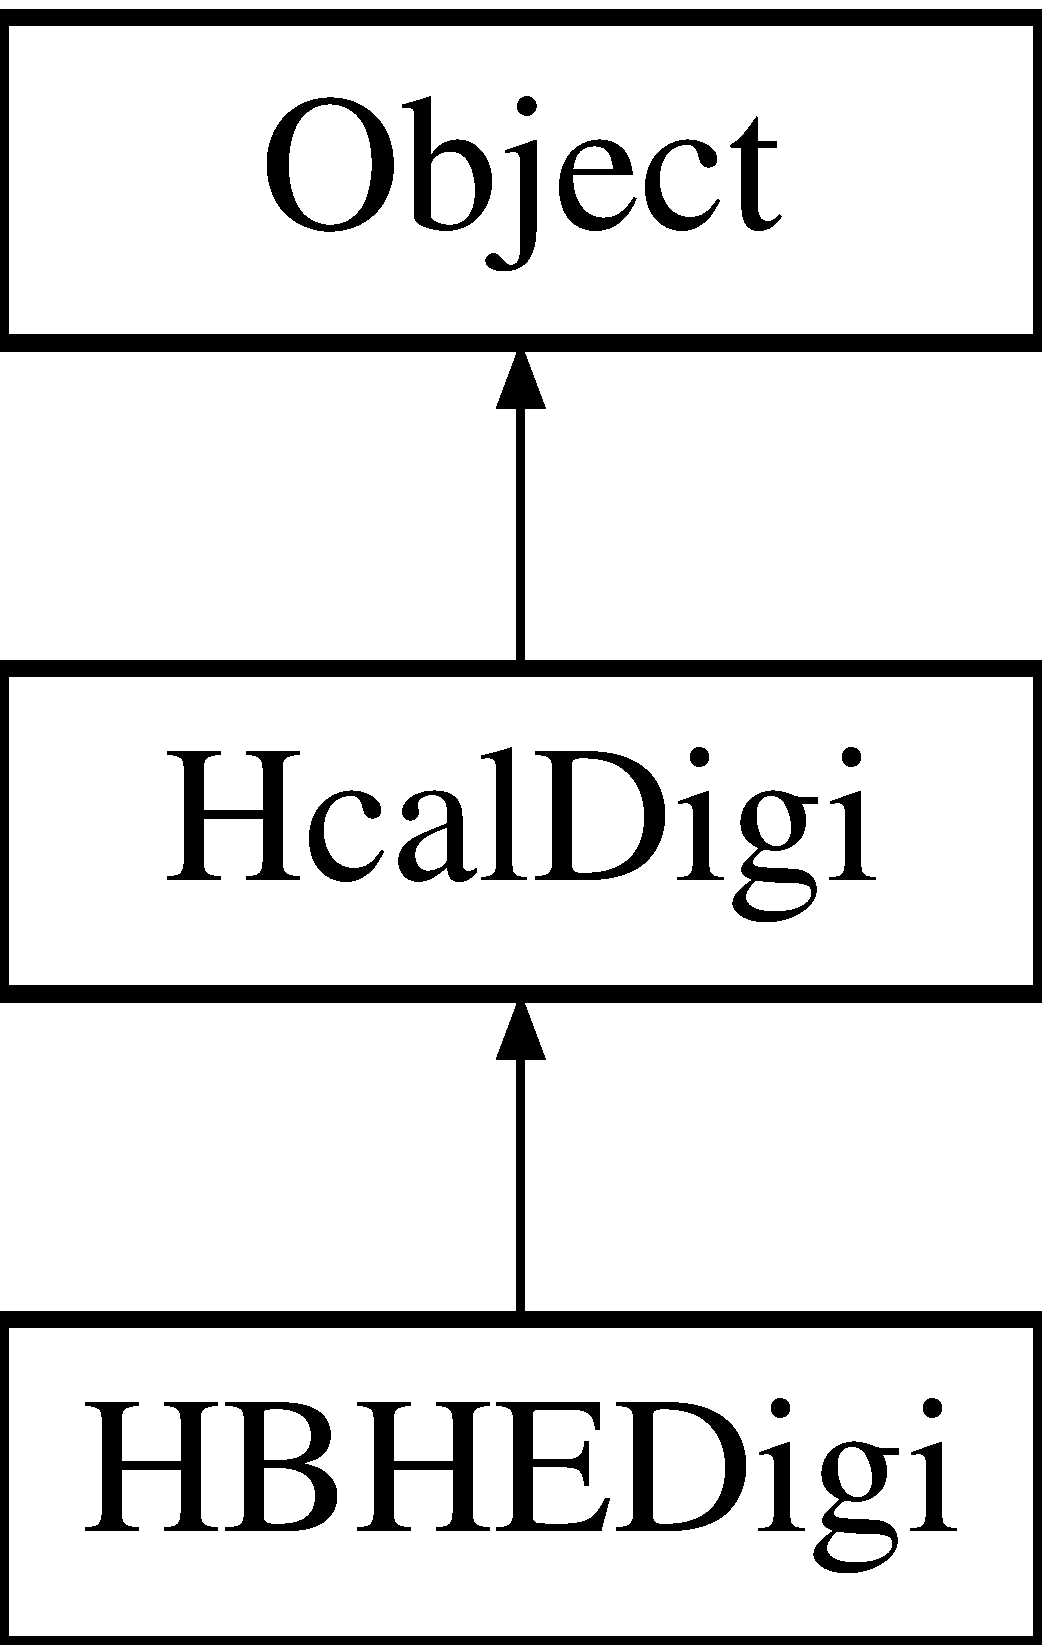
\includegraphics[height=3.000000cm]{class_h_b_h_e_digi}
\end{center}
\end{figure}
\subsection*{Public Member Functions}
\begin{DoxyCompactItemize}
\item 
\hyperlink{class_h_b_h_e_digi_ac4c70373431b860ab1b599905714343b}{H\+B\+H\+E\+Digi} ()
\item 
\hyperlink{class_h_b_h_e_digi_a35d6f6074781a2d0ec2ce357d24cb11e}{H\+B\+H\+E\+Digi} (\hyperlink{class_collection}{Collection} \&c, unsigned short i, short j=0)
\item 
float \hyperlink{class_h_b_h_e_digi_a0f5025749bcd77805e199893f22a3e68}{energy} ()
\item 
float \hyperlink{class_h_b_h_e_digi_aecd2a59dcb215797ba559c75da4cd2f4}{rec\+Hit\+Time} ()
\item 
int \hyperlink{class_h_b_h_e_digi_af21f90b00a2f6426b1a9fcdb9dc6df19}{ieta} ()
\item 
int \hyperlink{class_h_b_h_e_digi_a298eb50c54fa265c3b54da98273582e8}{iphi} ()
\item 
float \hyperlink{class_h_b_h_e_digi_ac916697a2097f0fa62cf22ef53aeddf6}{eta} ()
\item 
float \hyperlink{class_h_b_h_e_digi_a4378c44b806a6c52b42bf45a15d958c0}{phi} ()
\item 
int \hyperlink{class_h_b_h_e_digi_adb9be00df4f0020f7cd1fc40c3a84b3c}{depth} ()
\item 
int \hyperlink{class_h_b_h_e_digi_aa9e095b62d3f54e4be6dc8b1a9414a4a}{subdet} ()
\item 
int \hyperlink{class_h_b_h_e_digi_ae86275760fadb4c34a6a2371b71c7c99}{size} ()
\item 
int \hyperlink{class_h_b_h_e_digi_a8b5ebee824decc29577614aba1b1a6cf}{presamples} ()
\item 
int \hyperlink{class_h_b_h_e_digi_a2a7ab522d25e2441b7e9f42a14c8a28e}{electronics\+Id} ()
\item 
int \hyperlink{class_h_b_h_e_digi_a09aaedd7443322629a9acb7bff896a50}{raw\+Id} ()
\item 
float \hyperlink{class_h_b_h_e_digi_a6048dac0f0c0267c52355a5284cef7e4}{fc} (int i)
\item 
int \hyperlink{class_h_b_h_e_digi_a13245b123aa2a7b9a77783ef063a2e9e}{adc} (int i)
\item 
int \hyperlink{class_h_b_h_e_digi_a1dad223a353a80ebf729ece94d4a40ed}{dv} (int i)
\item 
int \hyperlink{class_h_b_h_e_digi_a4a0513d9ad713c7043c532bdd806fb1e}{er} (int i)
\item 
int \hyperlink{class_h_b_h_e_digi_ab1ae8ad47951f6368763a4c29cbf2412}{capid} (int i)
\item 
int \hyperlink{class_h_b_h_e_digi_a7c3890054c40ebfeafb5f83d0fad4b31}{get\+Raw\+Index} ()
\item 
\hyperlink{class_h_b_h_e_sample}{H\+B\+H\+E\+Sample} \hyperlink{class_h_b_h_e_digi_abe944356d1568a368d2f48053eb57316}{operator\mbox{[}$\,$\mbox{]}} (int i)
\end{DoxyCompactItemize}
\subsection*{Additional Inherited Members}


\subsection{Constructor \& Destructor Documentation}
\hypertarget{class_h_b_h_e_digi_ac4c70373431b860ab1b599905714343b}{}\index{H\+B\+H\+E\+Digi@{H\+B\+H\+E\+Digi}!H\+B\+H\+E\+Digi@{H\+B\+H\+E\+Digi}}
\index{H\+B\+H\+E\+Digi@{H\+B\+H\+E\+Digi}!H\+B\+H\+E\+Digi@{H\+B\+H\+E\+Digi}}
\subsubsection[{H\+B\+H\+E\+Digi()}]{\setlength{\rightskip}{0pt plus 5cm}H\+B\+H\+E\+Digi\+::\+H\+B\+H\+E\+Digi (
\begin{DoxyParamCaption}
{}
\end{DoxyParamCaption}
)}\label{class_h_b_h_e_digi_ac4c70373431b860ab1b599905714343b}
\hypertarget{class_h_b_h_e_digi_a35d6f6074781a2d0ec2ce357d24cb11e}{}\index{H\+B\+H\+E\+Digi@{H\+B\+H\+E\+Digi}!H\+B\+H\+E\+Digi@{H\+B\+H\+E\+Digi}}
\index{H\+B\+H\+E\+Digi@{H\+B\+H\+E\+Digi}!H\+B\+H\+E\+Digi@{H\+B\+H\+E\+Digi}}
\subsubsection[{H\+B\+H\+E\+Digi(\+Collection \&c, unsigned short i, short j=0)}]{\setlength{\rightskip}{0pt plus 5cm}H\+B\+H\+E\+Digi\+::\+H\+B\+H\+E\+Digi (
\begin{DoxyParamCaption}
\item[{{\bf Collection} \&}]{c, }
\item[{unsigned short}]{i, }
\item[{short}]{j = {\ttfamily 0}}
\end{DoxyParamCaption}
)}\label{class_h_b_h_e_digi_a35d6f6074781a2d0ec2ce357d24cb11e}


\subsection{Member Function Documentation}
\hypertarget{class_h_b_h_e_digi_a13245b123aa2a7b9a77783ef063a2e9e}{}\index{H\+B\+H\+E\+Digi@{H\+B\+H\+E\+Digi}!adc@{adc}}
\index{adc@{adc}!H\+B\+H\+E\+Digi@{H\+B\+H\+E\+Digi}}
\subsubsection[{adc(int i)}]{\setlength{\rightskip}{0pt plus 5cm}int H\+B\+H\+E\+Digi\+::adc (
\begin{DoxyParamCaption}
\item[{int}]{i}
\end{DoxyParamCaption}
)\hspace{0.3cm}{\ttfamily [virtual]}}\label{class_h_b_h_e_digi_a13245b123aa2a7b9a77783ef063a2e9e}


Implements \hyperlink{class_hcal_digi_a737b46ab9bc5439f32232ee6911ed516}{Hcal\+Digi}.

\hypertarget{class_h_b_h_e_digi_ab1ae8ad47951f6368763a4c29cbf2412}{}\index{H\+B\+H\+E\+Digi@{H\+B\+H\+E\+Digi}!capid@{capid}}
\index{capid@{capid}!H\+B\+H\+E\+Digi@{H\+B\+H\+E\+Digi}}
\subsubsection[{capid(int i)}]{\setlength{\rightskip}{0pt plus 5cm}int H\+B\+H\+E\+Digi\+::capid (
\begin{DoxyParamCaption}
\item[{int}]{i}
\end{DoxyParamCaption}
)\hspace{0.3cm}{\ttfamily [virtual]}}\label{class_h_b_h_e_digi_ab1ae8ad47951f6368763a4c29cbf2412}


Implements \hyperlink{class_hcal_digi_ad6e205312dda117af660b9391d502155}{Hcal\+Digi}.

\hypertarget{class_h_b_h_e_digi_adb9be00df4f0020f7cd1fc40c3a84b3c}{}\index{H\+B\+H\+E\+Digi@{H\+B\+H\+E\+Digi}!depth@{depth}}
\index{depth@{depth}!H\+B\+H\+E\+Digi@{H\+B\+H\+E\+Digi}}
\subsubsection[{depth()}]{\setlength{\rightskip}{0pt plus 5cm}int H\+B\+H\+E\+Digi\+::depth (
\begin{DoxyParamCaption}
{}
\end{DoxyParamCaption}
)\hspace{0.3cm}{\ttfamily [virtual]}}\label{class_h_b_h_e_digi_adb9be00df4f0020f7cd1fc40c3a84b3c}


Implements \hyperlink{class_hcal_digi_a916a582b044a64e041ba38e545349f7f}{Hcal\+Digi}.

\hypertarget{class_h_b_h_e_digi_a1dad223a353a80ebf729ece94d4a40ed}{}\index{H\+B\+H\+E\+Digi@{H\+B\+H\+E\+Digi}!dv@{dv}}
\index{dv@{dv}!H\+B\+H\+E\+Digi@{H\+B\+H\+E\+Digi}}
\subsubsection[{dv(int i)}]{\setlength{\rightskip}{0pt plus 5cm}int H\+B\+H\+E\+Digi\+::dv (
\begin{DoxyParamCaption}
\item[{int}]{i}
\end{DoxyParamCaption}
)\hspace{0.3cm}{\ttfamily [virtual]}}\label{class_h_b_h_e_digi_a1dad223a353a80ebf729ece94d4a40ed}


Implements \hyperlink{class_hcal_digi_aa758519b70ab24ac4bb7635052cfa174}{Hcal\+Digi}.

\hypertarget{class_h_b_h_e_digi_a2a7ab522d25e2441b7e9f42a14c8a28e}{}\index{H\+B\+H\+E\+Digi@{H\+B\+H\+E\+Digi}!electronics\+Id@{electronics\+Id}}
\index{electronics\+Id@{electronics\+Id}!H\+B\+H\+E\+Digi@{H\+B\+H\+E\+Digi}}
\subsubsection[{electronics\+Id()}]{\setlength{\rightskip}{0pt plus 5cm}int H\+B\+H\+E\+Digi\+::electronics\+Id (
\begin{DoxyParamCaption}
{}
\end{DoxyParamCaption}
)\hspace{0.3cm}{\ttfamily [virtual]}}\label{class_h_b_h_e_digi_a2a7ab522d25e2441b7e9f42a14c8a28e}


Implements \hyperlink{class_hcal_digi_afc95a09767a731b098cb2e22b89cc4e0}{Hcal\+Digi}.

\hypertarget{class_h_b_h_e_digi_a0f5025749bcd77805e199893f22a3e68}{}\index{H\+B\+H\+E\+Digi@{H\+B\+H\+E\+Digi}!energy@{energy}}
\index{energy@{energy}!H\+B\+H\+E\+Digi@{H\+B\+H\+E\+Digi}}
\subsubsection[{energy()}]{\setlength{\rightskip}{0pt plus 5cm}float H\+B\+H\+E\+Digi\+::energy (
\begin{DoxyParamCaption}
{}
\end{DoxyParamCaption}
)\hspace{0.3cm}{\ttfamily [virtual]}}\label{class_h_b_h_e_digi_a0f5025749bcd77805e199893f22a3e68}


Implements \hyperlink{class_hcal_digi_a665c0fa940132fafc6dce9fd75f18cea}{Hcal\+Digi}.

\hypertarget{class_h_b_h_e_digi_a4a0513d9ad713c7043c532bdd806fb1e}{}\index{H\+B\+H\+E\+Digi@{H\+B\+H\+E\+Digi}!er@{er}}
\index{er@{er}!H\+B\+H\+E\+Digi@{H\+B\+H\+E\+Digi}}
\subsubsection[{er(int i)}]{\setlength{\rightskip}{0pt plus 5cm}int H\+B\+H\+E\+Digi\+::er (
\begin{DoxyParamCaption}
\item[{int}]{i}
\end{DoxyParamCaption}
)\hspace{0.3cm}{\ttfamily [virtual]}}\label{class_h_b_h_e_digi_a4a0513d9ad713c7043c532bdd806fb1e}


Implements \hyperlink{class_hcal_digi_a04b02a86692bcdff2fb8fa8c50cc0c34}{Hcal\+Digi}.

\hypertarget{class_h_b_h_e_digi_ac916697a2097f0fa62cf22ef53aeddf6}{}\index{H\+B\+H\+E\+Digi@{H\+B\+H\+E\+Digi}!eta@{eta}}
\index{eta@{eta}!H\+B\+H\+E\+Digi@{H\+B\+H\+E\+Digi}}
\subsubsection[{eta()}]{\setlength{\rightskip}{0pt plus 5cm}float H\+B\+H\+E\+Digi\+::eta (
\begin{DoxyParamCaption}
{}
\end{DoxyParamCaption}
)}\label{class_h_b_h_e_digi_ac916697a2097f0fa62cf22ef53aeddf6}
\hypertarget{class_h_b_h_e_digi_a6048dac0f0c0267c52355a5284cef7e4}{}\index{H\+B\+H\+E\+Digi@{H\+B\+H\+E\+Digi}!fc@{fc}}
\index{fc@{fc}!H\+B\+H\+E\+Digi@{H\+B\+H\+E\+Digi}}
\subsubsection[{fc(int i)}]{\setlength{\rightskip}{0pt plus 5cm}float H\+B\+H\+E\+Digi\+::fc (
\begin{DoxyParamCaption}
\item[{int}]{i}
\end{DoxyParamCaption}
)\hspace{0.3cm}{\ttfamily [virtual]}}\label{class_h_b_h_e_digi_a6048dac0f0c0267c52355a5284cef7e4}


Implements \hyperlink{class_hcal_digi_a4a5e45ca390ee81fe384bf4a7d05f1e0}{Hcal\+Digi}.

\hypertarget{class_h_b_h_e_digi_a7c3890054c40ebfeafb5f83d0fad4b31}{}\index{H\+B\+H\+E\+Digi@{H\+B\+H\+E\+Digi}!get\+Raw\+Index@{get\+Raw\+Index}}
\index{get\+Raw\+Index@{get\+Raw\+Index}!H\+B\+H\+E\+Digi@{H\+B\+H\+E\+Digi}}
\subsubsection[{get\+Raw\+Index()}]{\setlength{\rightskip}{0pt plus 5cm}int H\+B\+H\+E\+Digi\+::get\+Raw\+Index (
\begin{DoxyParamCaption}
{}
\end{DoxyParamCaption}
)\hspace{0.3cm}{\ttfamily [inline]}}\label{class_h_b_h_e_digi_a7c3890054c40ebfeafb5f83d0fad4b31}
\hypertarget{class_h_b_h_e_digi_af21f90b00a2f6426b1a9fcdb9dc6df19}{}\index{H\+B\+H\+E\+Digi@{H\+B\+H\+E\+Digi}!ieta@{ieta}}
\index{ieta@{ieta}!H\+B\+H\+E\+Digi@{H\+B\+H\+E\+Digi}}
\subsubsection[{ieta()}]{\setlength{\rightskip}{0pt plus 5cm}int H\+B\+H\+E\+Digi\+::ieta (
\begin{DoxyParamCaption}
{}
\end{DoxyParamCaption}
)\hspace{0.3cm}{\ttfamily [virtual]}}\label{class_h_b_h_e_digi_af21f90b00a2f6426b1a9fcdb9dc6df19}


Implements \hyperlink{class_hcal_digi_a65fc605c5c3bca7f78d961400d145c94}{Hcal\+Digi}.

\hypertarget{class_h_b_h_e_digi_a298eb50c54fa265c3b54da98273582e8}{}\index{H\+B\+H\+E\+Digi@{H\+B\+H\+E\+Digi}!iphi@{iphi}}
\index{iphi@{iphi}!H\+B\+H\+E\+Digi@{H\+B\+H\+E\+Digi}}
\subsubsection[{iphi()}]{\setlength{\rightskip}{0pt plus 5cm}int H\+B\+H\+E\+Digi\+::iphi (
\begin{DoxyParamCaption}
{}
\end{DoxyParamCaption}
)\hspace{0.3cm}{\ttfamily [virtual]}}\label{class_h_b_h_e_digi_a298eb50c54fa265c3b54da98273582e8}


Implements \hyperlink{class_hcal_digi_a979dec4585c9d07a7dc4060dfb97f089}{Hcal\+Digi}.

\hypertarget{class_h_b_h_e_digi_abe944356d1568a368d2f48053eb57316}{}\index{H\+B\+H\+E\+Digi@{H\+B\+H\+E\+Digi}!operator\mbox{[}$\,$\mbox{]}@{operator[]}}
\index{operator\mbox{[}$\,$\mbox{]}@{operator[]}!H\+B\+H\+E\+Digi@{H\+B\+H\+E\+Digi}}
\subsubsection[{operator[](int i)}]{\setlength{\rightskip}{0pt plus 5cm}{\bf H\+B\+H\+E\+Sample} H\+B\+H\+E\+Digi\+::operator\mbox{[}$\,$\mbox{]} (
\begin{DoxyParamCaption}
\item[{int}]{i}
\end{DoxyParamCaption}
)\hspace{0.3cm}{\ttfamily [inline]}}\label{class_h_b_h_e_digi_abe944356d1568a368d2f48053eb57316}
\hypertarget{class_h_b_h_e_digi_a4378c44b806a6c52b42bf45a15d958c0}{}\index{H\+B\+H\+E\+Digi@{H\+B\+H\+E\+Digi}!phi@{phi}}
\index{phi@{phi}!H\+B\+H\+E\+Digi@{H\+B\+H\+E\+Digi}}
\subsubsection[{phi()}]{\setlength{\rightskip}{0pt plus 5cm}float H\+B\+H\+E\+Digi\+::phi (
\begin{DoxyParamCaption}
{}
\end{DoxyParamCaption}
)}\label{class_h_b_h_e_digi_a4378c44b806a6c52b42bf45a15d958c0}
\hypertarget{class_h_b_h_e_digi_a8b5ebee824decc29577614aba1b1a6cf}{}\index{H\+B\+H\+E\+Digi@{H\+B\+H\+E\+Digi}!presamples@{presamples}}
\index{presamples@{presamples}!H\+B\+H\+E\+Digi@{H\+B\+H\+E\+Digi}}
\subsubsection[{presamples()}]{\setlength{\rightskip}{0pt plus 5cm}int H\+B\+H\+E\+Digi\+::presamples (
\begin{DoxyParamCaption}
{}
\end{DoxyParamCaption}
)\hspace{0.3cm}{\ttfamily [virtual]}}\label{class_h_b_h_e_digi_a8b5ebee824decc29577614aba1b1a6cf}


Implements \hyperlink{class_hcal_digi_aad0fc232379d8bdd40d6be32b3c980c4}{Hcal\+Digi}.

\hypertarget{class_h_b_h_e_digi_a09aaedd7443322629a9acb7bff896a50}{}\index{H\+B\+H\+E\+Digi@{H\+B\+H\+E\+Digi}!raw\+Id@{raw\+Id}}
\index{raw\+Id@{raw\+Id}!H\+B\+H\+E\+Digi@{H\+B\+H\+E\+Digi}}
\subsubsection[{raw\+Id()}]{\setlength{\rightskip}{0pt plus 5cm}int H\+B\+H\+E\+Digi\+::raw\+Id (
\begin{DoxyParamCaption}
{}
\end{DoxyParamCaption}
)\hspace{0.3cm}{\ttfamily [virtual]}}\label{class_h_b_h_e_digi_a09aaedd7443322629a9acb7bff896a50}


Implements \hyperlink{class_hcal_digi_aba55732d16499ad510091c769807f8e1}{Hcal\+Digi}.

\hypertarget{class_h_b_h_e_digi_aecd2a59dcb215797ba559c75da4cd2f4}{}\index{H\+B\+H\+E\+Digi@{H\+B\+H\+E\+Digi}!rec\+Hit\+Time@{rec\+Hit\+Time}}
\index{rec\+Hit\+Time@{rec\+Hit\+Time}!H\+B\+H\+E\+Digi@{H\+B\+H\+E\+Digi}}
\subsubsection[{rec\+Hit\+Time()}]{\setlength{\rightskip}{0pt plus 5cm}float H\+B\+H\+E\+Digi\+::rec\+Hit\+Time (
\begin{DoxyParamCaption}
{}
\end{DoxyParamCaption}
)\hspace{0.3cm}{\ttfamily [virtual]}}\label{class_h_b_h_e_digi_aecd2a59dcb215797ba559c75da4cd2f4}


Implements \hyperlink{class_hcal_digi_a3936cda623fc7535ed35d8d1c6abb350}{Hcal\+Digi}.

\hypertarget{class_h_b_h_e_digi_ae86275760fadb4c34a6a2371b71c7c99}{}\index{H\+B\+H\+E\+Digi@{H\+B\+H\+E\+Digi}!size@{size}}
\index{size@{size}!H\+B\+H\+E\+Digi@{H\+B\+H\+E\+Digi}}
\subsubsection[{size()}]{\setlength{\rightskip}{0pt plus 5cm}int H\+B\+H\+E\+Digi\+::size (
\begin{DoxyParamCaption}
{}
\end{DoxyParamCaption}
)\hspace{0.3cm}{\ttfamily [virtual]}}\label{class_h_b_h_e_digi_ae86275760fadb4c34a6a2371b71c7c99}


Implements \hyperlink{class_hcal_digi_a054f6f17539c8042d2900144d06eb4fc}{Hcal\+Digi}.

\hypertarget{class_h_b_h_e_digi_aa9e095b62d3f54e4be6dc8b1a9414a4a}{}\index{H\+B\+H\+E\+Digi@{H\+B\+H\+E\+Digi}!subdet@{subdet}}
\index{subdet@{subdet}!H\+B\+H\+E\+Digi@{H\+B\+H\+E\+Digi}}
\subsubsection[{subdet()}]{\setlength{\rightskip}{0pt plus 5cm}int H\+B\+H\+E\+Digi\+::subdet (
\begin{DoxyParamCaption}
{}
\end{DoxyParamCaption}
)}\label{class_h_b_h_e_digi_aa9e095b62d3f54e4be6dc8b1a9414a4a}


The documentation for this class was generated from the following files\+:\begin{DoxyCompactItemize}
\item 
interface/\hyperlink{_h_b_h_e_digi_8h}{H\+B\+H\+E\+Digi.\+h}\item 
src/\hyperlink{_h_b_h_e_digi_8cc}{H\+B\+H\+E\+Digi.\+cc}\end{DoxyCompactItemize}

\hypertarget{class_h_b_h_e_sample}{}\section{H\+B\+H\+E\+Sample Class Reference}
\label{class_h_b_h_e_sample}\index{H\+B\+H\+E\+Sample@{H\+B\+H\+E\+Sample}}


{\ttfamily \#include $<$H\+B\+H\+E\+Sample.\+h$>$}

Inheritance diagram for H\+B\+H\+E\+Sample\+:\begin{figure}[H]
\begin{center}
\leavevmode
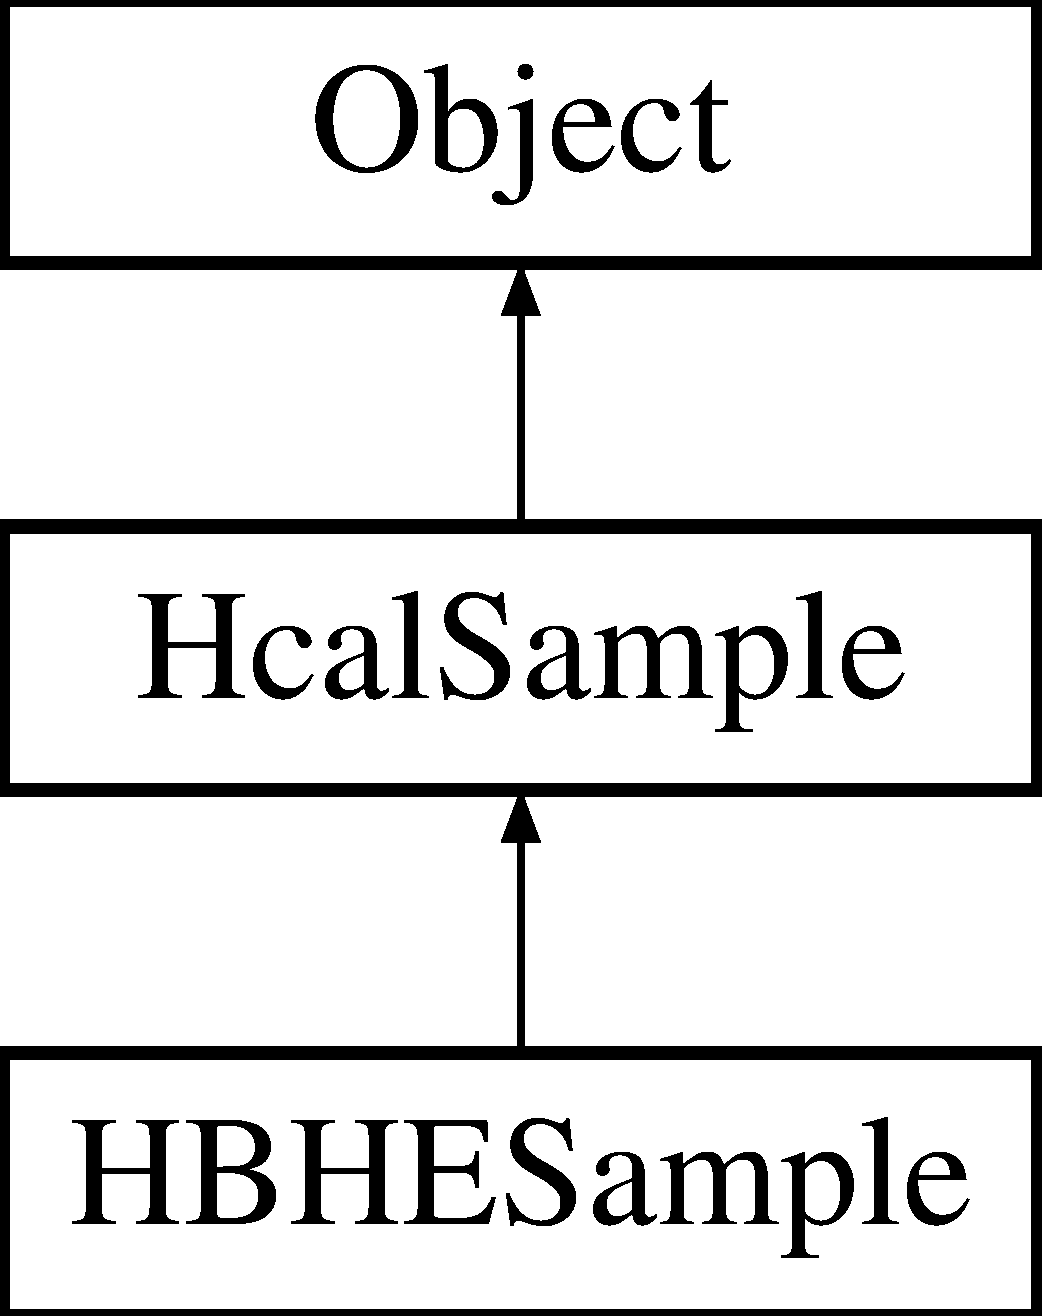
\includegraphics[height=3.000000cm]{class_h_b_h_e_sample}
\end{center}
\end{figure}
\subsection*{Public Member Functions}
\begin{DoxyCompactItemize}
\item 
\hyperlink{class_h_b_h_e_sample_adb1c7ad526bc02a95c01a82e387e3909}{H\+B\+H\+E\+Sample} ()
\item 
\hyperlink{class_h_b_h_e_sample_a04ae168af41f9b0a1588ce77b934c0e5}{H\+B\+H\+E\+Sample} (\hyperlink{class_collection}{Collection} \&c, unsigned short i, short j)
\item 
float \hyperlink{class_h_b_h_e_sample_ac674f791c79264801dbedd14c2cd88c7}{all\+F\+C} ()
\item 
float \hyperlink{class_h_b_h_e_sample_aaf6e464f53e1927e8c81c9d45bf5edd7}{energy} ()
\item 
float \hyperlink{class_h_b_h_e_sample_a213cba0c1dfac7f9c81e4bb89d1a096d}{gain} ()
\item 
float \hyperlink{class_h_b_h_e_sample_acb53267f00c5eda17d44e8e08cd97752}{fc} ()
\item 
float \hyperlink{class_h_b_h_e_sample_a1dffd426b564378da4161b5279da97b6}{nom\+F\+C} ()
\item 
float \hyperlink{class_h_b_h_e_sample_afeaa57de45b3ad755e91ba154adf9c78}{ped\+F\+C} ()
\item 
float \hyperlink{class_h_b_h_e_sample_ab03c24466f72bce782a3fcf62df15e5f}{rc\+Gain} ()
\item 
int \hyperlink{class_h_b_h_e_sample_a0519407431ebef16ff6e1df63551b99f}{adc} ()
\item 
int \hyperlink{class_h_b_h_e_sample_a8422a9d26a2ee570186192bf8bb32d13}{capid} ()
\item 
int \hyperlink{class_h_b_h_e_sample_a3baa7c7a60db7c5e01ed8d5861cb2093}{dv} ()
\item 
int \hyperlink{class_h_b_h_e_sample_a54f776ae3bda86074cc5449871588b8c}{er} ()
\item 
int \hyperlink{class_h_b_h_e_sample_a65cb719fc34ef056908006c63dc1e35f}{fiber} ()
\item 
int \hyperlink{class_h_b_h_e_sample_a87b6f6251cf487f49f98e914938cd26b}{fiber\+Chan} ()
\item 
int \hyperlink{class_h_b_h_e_sample_ac72e5201bf29d9460694bf65311ba9b7}{raw} ()
\item 
int \hyperlink{class_h_b_h_e_sample_acaa1246c5285f24db1f5317481d98e6f}{get\+Raw\+Index} ()
\item 
int \hyperlink{class_h_b_h_e_sample_a2a4edc2a272e650c7d78377d1d98db80}{get\+Time\+Slice} ()
\end{DoxyCompactItemize}
\subsection*{Additional Inherited Members}


\subsection{Constructor \& Destructor Documentation}
\hypertarget{class_h_b_h_e_sample_adb1c7ad526bc02a95c01a82e387e3909}{}\index{H\+B\+H\+E\+Sample@{H\+B\+H\+E\+Sample}!H\+B\+H\+E\+Sample@{H\+B\+H\+E\+Sample}}
\index{H\+B\+H\+E\+Sample@{H\+B\+H\+E\+Sample}!H\+B\+H\+E\+Sample@{H\+B\+H\+E\+Sample}}
\subsubsection[{H\+B\+H\+E\+Sample()}]{\setlength{\rightskip}{0pt plus 5cm}H\+B\+H\+E\+Sample\+::\+H\+B\+H\+E\+Sample (
\begin{DoxyParamCaption}
{}
\end{DoxyParamCaption}
)}\label{class_h_b_h_e_sample_adb1c7ad526bc02a95c01a82e387e3909}
\hypertarget{class_h_b_h_e_sample_a04ae168af41f9b0a1588ce77b934c0e5}{}\index{H\+B\+H\+E\+Sample@{H\+B\+H\+E\+Sample}!H\+B\+H\+E\+Sample@{H\+B\+H\+E\+Sample}}
\index{H\+B\+H\+E\+Sample@{H\+B\+H\+E\+Sample}!H\+B\+H\+E\+Sample@{H\+B\+H\+E\+Sample}}
\subsubsection[{H\+B\+H\+E\+Sample(\+Collection \&c, unsigned short i, short j)}]{\setlength{\rightskip}{0pt plus 5cm}H\+B\+H\+E\+Sample\+::\+H\+B\+H\+E\+Sample (
\begin{DoxyParamCaption}
\item[{{\bf Collection} \&}]{c, }
\item[{unsigned short}]{i, }
\item[{short}]{j}
\end{DoxyParamCaption}
)}\label{class_h_b_h_e_sample_a04ae168af41f9b0a1588ce77b934c0e5}


\subsection{Member Function Documentation}
\hypertarget{class_h_b_h_e_sample_a0519407431ebef16ff6e1df63551b99f}{}\index{H\+B\+H\+E\+Sample@{H\+B\+H\+E\+Sample}!adc@{adc}}
\index{adc@{adc}!H\+B\+H\+E\+Sample@{H\+B\+H\+E\+Sample}}
\subsubsection[{adc()}]{\setlength{\rightskip}{0pt plus 5cm}int H\+B\+H\+E\+Sample\+::adc (
\begin{DoxyParamCaption}
{}
\end{DoxyParamCaption}
)\hspace{0.3cm}{\ttfamily [virtual]}}\label{class_h_b_h_e_sample_a0519407431ebef16ff6e1df63551b99f}


Implements \hyperlink{class_hcal_sample_a3801777ac080ca0e512c226e4cfd5682}{Hcal\+Sample}.

\hypertarget{class_h_b_h_e_sample_ac674f791c79264801dbedd14c2cd88c7}{}\index{H\+B\+H\+E\+Sample@{H\+B\+H\+E\+Sample}!all\+F\+C@{all\+F\+C}}
\index{all\+F\+C@{all\+F\+C}!H\+B\+H\+E\+Sample@{H\+B\+H\+E\+Sample}}
\subsubsection[{all\+F\+C()}]{\setlength{\rightskip}{0pt plus 5cm}float H\+B\+H\+E\+Sample\+::all\+F\+C (
\begin{DoxyParamCaption}
{}
\end{DoxyParamCaption}
)\hspace{0.3cm}{\ttfamily [virtual]}}\label{class_h_b_h_e_sample_ac674f791c79264801dbedd14c2cd88c7}


Implements \hyperlink{class_hcal_sample_af837bd894eb8eae865023a526940ee15}{Hcal\+Sample}.

\hypertarget{class_h_b_h_e_sample_a8422a9d26a2ee570186192bf8bb32d13}{}\index{H\+B\+H\+E\+Sample@{H\+B\+H\+E\+Sample}!capid@{capid}}
\index{capid@{capid}!H\+B\+H\+E\+Sample@{H\+B\+H\+E\+Sample}}
\subsubsection[{capid()}]{\setlength{\rightskip}{0pt plus 5cm}int H\+B\+H\+E\+Sample\+::capid (
\begin{DoxyParamCaption}
{}
\end{DoxyParamCaption}
)\hspace{0.3cm}{\ttfamily [virtual]}}\label{class_h_b_h_e_sample_a8422a9d26a2ee570186192bf8bb32d13}


Implements \hyperlink{class_hcal_sample_a51a82042ba140a68f9659140c48d83bc}{Hcal\+Sample}.

\hypertarget{class_h_b_h_e_sample_a3baa7c7a60db7c5e01ed8d5861cb2093}{}\index{H\+B\+H\+E\+Sample@{H\+B\+H\+E\+Sample}!dv@{dv}}
\index{dv@{dv}!H\+B\+H\+E\+Sample@{H\+B\+H\+E\+Sample}}
\subsubsection[{dv()}]{\setlength{\rightskip}{0pt plus 5cm}int H\+B\+H\+E\+Sample\+::dv (
\begin{DoxyParamCaption}
{}
\end{DoxyParamCaption}
)\hspace{0.3cm}{\ttfamily [virtual]}}\label{class_h_b_h_e_sample_a3baa7c7a60db7c5e01ed8d5861cb2093}


Implements \hyperlink{class_hcal_sample_a13c0e851a42d3122c7bba32d81e31d19}{Hcal\+Sample}.

\hypertarget{class_h_b_h_e_sample_aaf6e464f53e1927e8c81c9d45bf5edd7}{}\index{H\+B\+H\+E\+Sample@{H\+B\+H\+E\+Sample}!energy@{energy}}
\index{energy@{energy}!H\+B\+H\+E\+Sample@{H\+B\+H\+E\+Sample}}
\subsubsection[{energy()}]{\setlength{\rightskip}{0pt plus 5cm}float H\+B\+H\+E\+Sample\+::energy (
\begin{DoxyParamCaption}
{}
\end{DoxyParamCaption}
)\hspace{0.3cm}{\ttfamily [virtual]}}\label{class_h_b_h_e_sample_aaf6e464f53e1927e8c81c9d45bf5edd7}


Implements \hyperlink{class_hcal_sample_a603c4e95d1d49db37dd00f34275fb8f3}{Hcal\+Sample}.

\hypertarget{class_h_b_h_e_sample_a54f776ae3bda86074cc5449871588b8c}{}\index{H\+B\+H\+E\+Sample@{H\+B\+H\+E\+Sample}!er@{er}}
\index{er@{er}!H\+B\+H\+E\+Sample@{H\+B\+H\+E\+Sample}}
\subsubsection[{er()}]{\setlength{\rightskip}{0pt plus 5cm}int H\+B\+H\+E\+Sample\+::er (
\begin{DoxyParamCaption}
{}
\end{DoxyParamCaption}
)\hspace{0.3cm}{\ttfamily [virtual]}}\label{class_h_b_h_e_sample_a54f776ae3bda86074cc5449871588b8c}


Implements \hyperlink{class_hcal_sample_af1805d239ccbc17a6c307d66522da618}{Hcal\+Sample}.

\hypertarget{class_h_b_h_e_sample_acb53267f00c5eda17d44e8e08cd97752}{}\index{H\+B\+H\+E\+Sample@{H\+B\+H\+E\+Sample}!fc@{fc}}
\index{fc@{fc}!H\+B\+H\+E\+Sample@{H\+B\+H\+E\+Sample}}
\subsubsection[{fc()}]{\setlength{\rightskip}{0pt plus 5cm}float H\+B\+H\+E\+Sample\+::fc (
\begin{DoxyParamCaption}
{}
\end{DoxyParamCaption}
)\hspace{0.3cm}{\ttfamily [virtual]}}\label{class_h_b_h_e_sample_acb53267f00c5eda17d44e8e08cd97752}


Implements \hyperlink{class_hcal_sample_aed932c9f932eabed9f9bc6b1a54c20dd}{Hcal\+Sample}.

\hypertarget{class_h_b_h_e_sample_a65cb719fc34ef056908006c63dc1e35f}{}\index{H\+B\+H\+E\+Sample@{H\+B\+H\+E\+Sample}!fiber@{fiber}}
\index{fiber@{fiber}!H\+B\+H\+E\+Sample@{H\+B\+H\+E\+Sample}}
\subsubsection[{fiber()}]{\setlength{\rightskip}{0pt plus 5cm}int H\+B\+H\+E\+Sample\+::fiber (
\begin{DoxyParamCaption}
{}
\end{DoxyParamCaption}
)\hspace{0.3cm}{\ttfamily [virtual]}}\label{class_h_b_h_e_sample_a65cb719fc34ef056908006c63dc1e35f}


Implements \hyperlink{class_hcal_sample_a5ae9a4d213b69f5ee382c7a6b31eb446}{Hcal\+Sample}.

\hypertarget{class_h_b_h_e_sample_a87b6f6251cf487f49f98e914938cd26b}{}\index{H\+B\+H\+E\+Sample@{H\+B\+H\+E\+Sample}!fiber\+Chan@{fiber\+Chan}}
\index{fiber\+Chan@{fiber\+Chan}!H\+B\+H\+E\+Sample@{H\+B\+H\+E\+Sample}}
\subsubsection[{fiber\+Chan()}]{\setlength{\rightskip}{0pt plus 5cm}int H\+B\+H\+E\+Sample\+::fiber\+Chan (
\begin{DoxyParamCaption}
{}
\end{DoxyParamCaption}
)\hspace{0.3cm}{\ttfamily [virtual]}}\label{class_h_b_h_e_sample_a87b6f6251cf487f49f98e914938cd26b}


Implements \hyperlink{class_hcal_sample_acdd36acaedfe4e1a6114e6c56d1ed996}{Hcal\+Sample}.

\hypertarget{class_h_b_h_e_sample_a213cba0c1dfac7f9c81e4bb89d1a096d}{}\index{H\+B\+H\+E\+Sample@{H\+B\+H\+E\+Sample}!gain@{gain}}
\index{gain@{gain}!H\+B\+H\+E\+Sample@{H\+B\+H\+E\+Sample}}
\subsubsection[{gain()}]{\setlength{\rightskip}{0pt plus 5cm}float H\+B\+H\+E\+Sample\+::gain (
\begin{DoxyParamCaption}
{}
\end{DoxyParamCaption}
)\hspace{0.3cm}{\ttfamily [virtual]}}\label{class_h_b_h_e_sample_a213cba0c1dfac7f9c81e4bb89d1a096d}


Implements \hyperlink{class_hcal_sample_aefc3dd058b3b178917583ca6abbf4f01}{Hcal\+Sample}.

\hypertarget{class_h_b_h_e_sample_acaa1246c5285f24db1f5317481d98e6f}{}\index{H\+B\+H\+E\+Sample@{H\+B\+H\+E\+Sample}!get\+Raw\+Index@{get\+Raw\+Index}}
\index{get\+Raw\+Index@{get\+Raw\+Index}!H\+B\+H\+E\+Sample@{H\+B\+H\+E\+Sample}}
\subsubsection[{get\+Raw\+Index()}]{\setlength{\rightskip}{0pt plus 5cm}int H\+B\+H\+E\+Sample\+::get\+Raw\+Index (
\begin{DoxyParamCaption}
{}
\end{DoxyParamCaption}
)\hspace{0.3cm}{\ttfamily [inline]}}\label{class_h_b_h_e_sample_acaa1246c5285f24db1f5317481d98e6f}
\hypertarget{class_h_b_h_e_sample_a2a4edc2a272e650c7d78377d1d98db80}{}\index{H\+B\+H\+E\+Sample@{H\+B\+H\+E\+Sample}!get\+Time\+Slice@{get\+Time\+Slice}}
\index{get\+Time\+Slice@{get\+Time\+Slice}!H\+B\+H\+E\+Sample@{H\+B\+H\+E\+Sample}}
\subsubsection[{get\+Time\+Slice()}]{\setlength{\rightskip}{0pt plus 5cm}int H\+B\+H\+E\+Sample\+::get\+Time\+Slice (
\begin{DoxyParamCaption}
{}
\end{DoxyParamCaption}
)\hspace{0.3cm}{\ttfamily [inline]}}\label{class_h_b_h_e_sample_a2a4edc2a272e650c7d78377d1d98db80}
\hypertarget{class_h_b_h_e_sample_a1dffd426b564378da4161b5279da97b6}{}\index{H\+B\+H\+E\+Sample@{H\+B\+H\+E\+Sample}!nom\+F\+C@{nom\+F\+C}}
\index{nom\+F\+C@{nom\+F\+C}!H\+B\+H\+E\+Sample@{H\+B\+H\+E\+Sample}}
\subsubsection[{nom\+F\+C()}]{\setlength{\rightskip}{0pt plus 5cm}float H\+B\+H\+E\+Sample\+::nom\+F\+C (
\begin{DoxyParamCaption}
{}
\end{DoxyParamCaption}
)\hspace{0.3cm}{\ttfamily [virtual]}}\label{class_h_b_h_e_sample_a1dffd426b564378da4161b5279da97b6}


Implements \hyperlink{class_hcal_sample_a9f47a5b867c94c97c3d553e244e7dc87}{Hcal\+Sample}.

\hypertarget{class_h_b_h_e_sample_afeaa57de45b3ad755e91ba154adf9c78}{}\index{H\+B\+H\+E\+Sample@{H\+B\+H\+E\+Sample}!ped\+F\+C@{ped\+F\+C}}
\index{ped\+F\+C@{ped\+F\+C}!H\+B\+H\+E\+Sample@{H\+B\+H\+E\+Sample}}
\subsubsection[{ped\+F\+C()}]{\setlength{\rightskip}{0pt plus 5cm}float H\+B\+H\+E\+Sample\+::ped\+F\+C (
\begin{DoxyParamCaption}
{}
\end{DoxyParamCaption}
)\hspace{0.3cm}{\ttfamily [virtual]}}\label{class_h_b_h_e_sample_afeaa57de45b3ad755e91ba154adf9c78}


Implements \hyperlink{class_hcal_sample_a471f7ef87944ac870ea884a0cc957744}{Hcal\+Sample}.

\hypertarget{class_h_b_h_e_sample_ac72e5201bf29d9460694bf65311ba9b7}{}\index{H\+B\+H\+E\+Sample@{H\+B\+H\+E\+Sample}!raw@{raw}}
\index{raw@{raw}!H\+B\+H\+E\+Sample@{H\+B\+H\+E\+Sample}}
\subsubsection[{raw()}]{\setlength{\rightskip}{0pt plus 5cm}int H\+B\+H\+E\+Sample\+::raw (
\begin{DoxyParamCaption}
{}
\end{DoxyParamCaption}
)\hspace{0.3cm}{\ttfamily [virtual]}}\label{class_h_b_h_e_sample_ac72e5201bf29d9460694bf65311ba9b7}


Implements \hyperlink{class_hcal_sample_a328a0f8f80a0aae47a92500297635bd6}{Hcal\+Sample}.

\hypertarget{class_h_b_h_e_sample_ab03c24466f72bce782a3fcf62df15e5f}{}\index{H\+B\+H\+E\+Sample@{H\+B\+H\+E\+Sample}!rc\+Gain@{rc\+Gain}}
\index{rc\+Gain@{rc\+Gain}!H\+B\+H\+E\+Sample@{H\+B\+H\+E\+Sample}}
\subsubsection[{rc\+Gain()}]{\setlength{\rightskip}{0pt plus 5cm}float H\+B\+H\+E\+Sample\+::rc\+Gain (
\begin{DoxyParamCaption}
{}
\end{DoxyParamCaption}
)\hspace{0.3cm}{\ttfamily [virtual]}}\label{class_h_b_h_e_sample_ab03c24466f72bce782a3fcf62df15e5f}


Implements \hyperlink{class_hcal_sample_a6fd32da2d5ea80154251de366f98c49c}{Hcal\+Sample}.



The documentation for this class was generated from the following files\+:\begin{DoxyCompactItemize}
\item 
interface/\hyperlink{_h_b_h_e_sample_8h}{H\+B\+H\+E\+Sample.\+h}\item 
src/\hyperlink{_h_b_h_e_sample_8cc}{H\+B\+H\+E\+Sample.\+cc}\end{DoxyCompactItemize}

\hypertarget{class_h_b_h_e_u_t_c_a}{}\section{H\+B\+H\+E\+U\+T\+C\+A Class Reference}
\label{class_h_b_h_e_u_t_c_a}\index{H\+B\+H\+E\+U\+T\+C\+A@{H\+B\+H\+E\+U\+T\+C\+A}}


{\ttfamily \#include $<$H\+B\+H\+E\+U\+T\+C\+A.\+h$>$}

Inheritance diagram for H\+B\+H\+E\+U\+T\+C\+A\+:\begin{figure}[H]
\begin{center}
\leavevmode
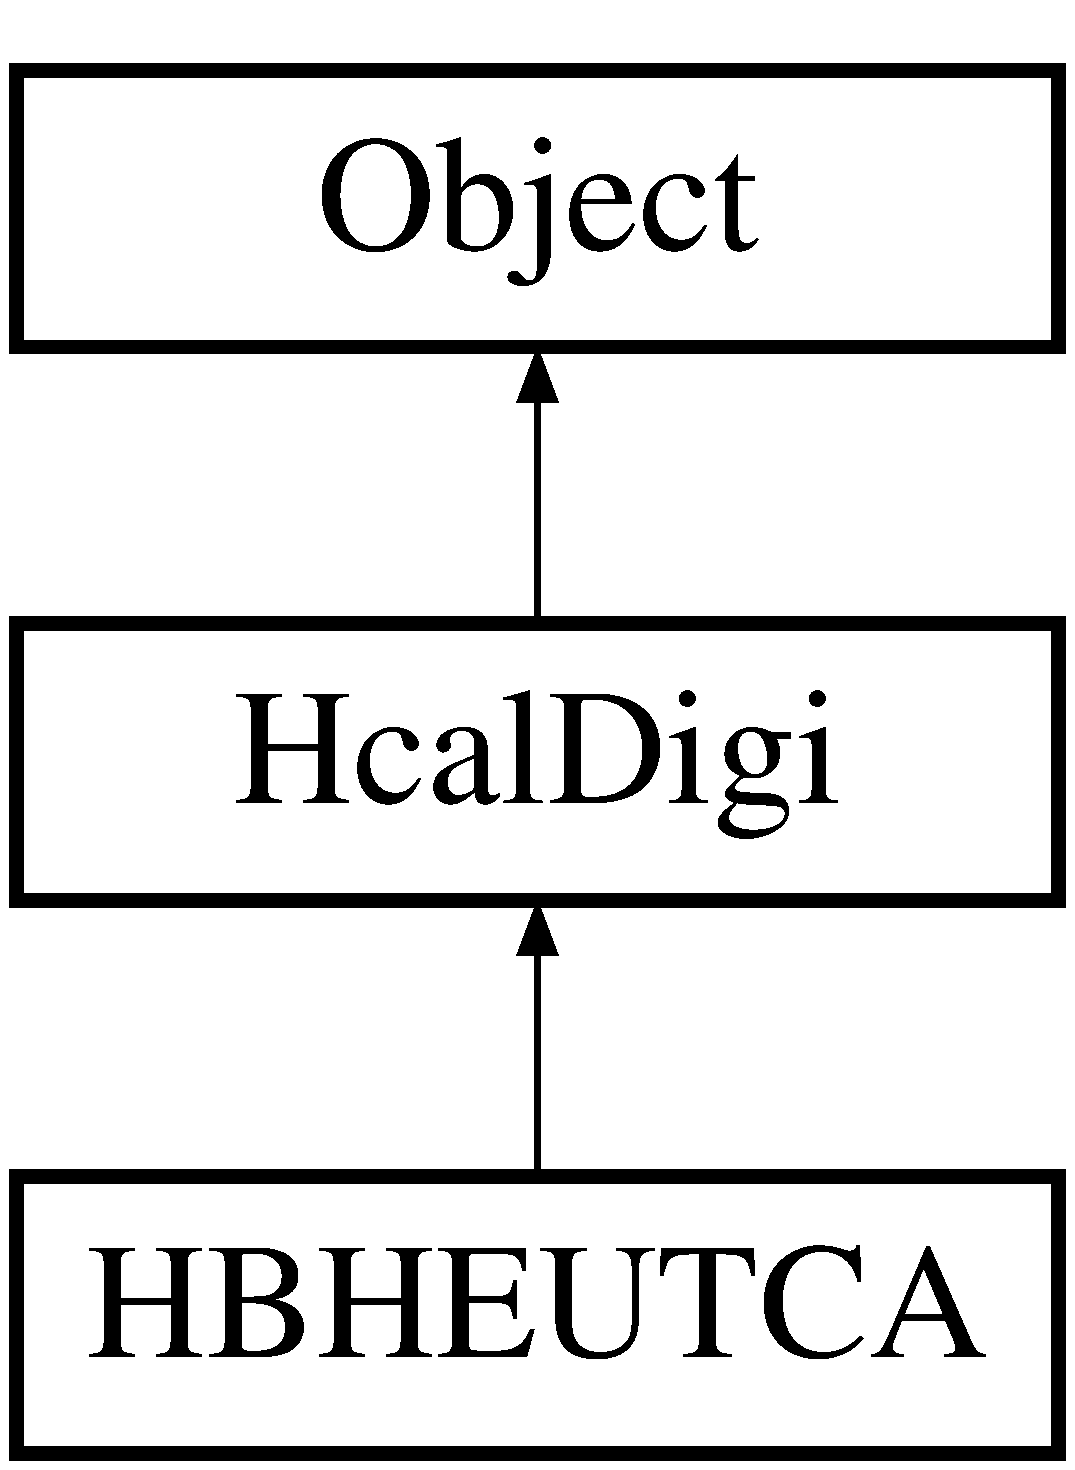
\includegraphics[height=3.000000cm]{class_h_b_h_e_u_t_c_a}
\end{center}
\end{figure}
\subsection*{Public Member Functions}
\begin{DoxyCompactItemize}
\item 
\hyperlink{class_h_b_h_e_u_t_c_a_a8bb7c04c0aaef5ac329bb2ab58c68606}{H\+B\+H\+E\+U\+T\+C\+A} ()
\item 
\hyperlink{class_h_b_h_e_u_t_c_a_aaf14978345ef0227706c297e98179a44}{H\+B\+H\+E\+U\+T\+C\+A} (\hyperlink{class_collection}{Collection} \&c, unsigned short i, short j=0)
\item 
float \hyperlink{class_h_b_h_e_u_t_c_a_a90f3f6a187dfc4a7daab1eec62403a11}{energy} ()
\item 
float \hyperlink{class_h_b_h_e_u_t_c_a_aff798ca66309c09608573f0c4a0deaff}{rec\+Hit\+Time} ()
\item 
int \hyperlink{class_h_b_h_e_u_t_c_a_a58e2f67223522ef6b3722e05cd9f27e2}{ieta} ()
\item 
int \hyperlink{class_h_b_h_e_u_t_c_a_a8a18a62e86b585d657450032fd4a364b}{iphi} ()
\item 
int \hyperlink{class_h_b_h_e_u_t_c_a_aeaf0cb6c915c4eb6ff434d8958a89dcb}{depth} ()
\item 
int \hyperlink{class_h_b_h_e_u_t_c_a_aa7a56c86797c67add0f34999e3d7b69d}{size} ()
\item 
int \hyperlink{class_h_b_h_e_u_t_c_a_a4a4e3c399d97f65a0039fa564d03de06}{presamples} ()
\item 
int \hyperlink{class_h_b_h_e_u_t_c_a_a6a8cf86fb45a78134eb0a050760c40a1}{raw\+Id} ()
\item 
int \hyperlink{class_h_b_h_e_u_t_c_a_a38a9cae6397668a3193f94ec7b7228e7}{electronics\+Id} ()
\item 
float \hyperlink{class_h_b_h_e_u_t_c_a_ab20263c255cc955b2011c38fb0e65463}{fc} (int i)
\item 
int \hyperlink{class_h_b_h_e_u_t_c_a_abeffd6ef4e4023b16b3e34b4ee08946a}{adc} (int i)
\item 
int \hyperlink{class_h_b_h_e_u_t_c_a_a73c8777b58168a278e6232ade243feb5}{dv} (int i)
\item 
int \hyperlink{class_h_b_h_e_u_t_c_a_a43349b34a4d3fd699feb4b794b47edd8}{er} (int i)
\item 
int \hyperlink{class_h_b_h_e_u_t_c_a_ae7aa759c1fa1e23d7afe5f7041232cf0}{capid} (int i)
\item 
int \hyperlink{class_h_b_h_e_u_t_c_a_a8b496828bb0af26a060965c293bbaab2}{get\+Raw\+Index} ()
\item 
\hyperlink{class_h_b_h_e_u_t_c_a_sample}{H\+B\+H\+E\+U\+T\+C\+A\+Sample} \hyperlink{class_h_b_h_e_u_t_c_a_a038fc4d276ae07cb28d1a486e881433c}{operator\mbox{[}$\,$\mbox{]}} (int i)
\end{DoxyCompactItemize}
\subsection*{Additional Inherited Members}


\subsection{Constructor \& Destructor Documentation}
\hypertarget{class_h_b_h_e_u_t_c_a_a8bb7c04c0aaef5ac329bb2ab58c68606}{}\index{H\+B\+H\+E\+U\+T\+C\+A@{H\+B\+H\+E\+U\+T\+C\+A}!H\+B\+H\+E\+U\+T\+C\+A@{H\+B\+H\+E\+U\+T\+C\+A}}
\index{H\+B\+H\+E\+U\+T\+C\+A@{H\+B\+H\+E\+U\+T\+C\+A}!H\+B\+H\+E\+U\+T\+C\+A@{H\+B\+H\+E\+U\+T\+C\+A}}
\subsubsection[{H\+B\+H\+E\+U\+T\+C\+A()}]{\setlength{\rightskip}{0pt plus 5cm}H\+B\+H\+E\+U\+T\+C\+A\+::\+H\+B\+H\+E\+U\+T\+C\+A (
\begin{DoxyParamCaption}
{}
\end{DoxyParamCaption}
)}\label{class_h_b_h_e_u_t_c_a_a8bb7c04c0aaef5ac329bb2ab58c68606}
\hypertarget{class_h_b_h_e_u_t_c_a_aaf14978345ef0227706c297e98179a44}{}\index{H\+B\+H\+E\+U\+T\+C\+A@{H\+B\+H\+E\+U\+T\+C\+A}!H\+B\+H\+E\+U\+T\+C\+A@{H\+B\+H\+E\+U\+T\+C\+A}}
\index{H\+B\+H\+E\+U\+T\+C\+A@{H\+B\+H\+E\+U\+T\+C\+A}!H\+B\+H\+E\+U\+T\+C\+A@{H\+B\+H\+E\+U\+T\+C\+A}}
\subsubsection[{H\+B\+H\+E\+U\+T\+C\+A(\+Collection \&c, unsigned short i, short j=0)}]{\setlength{\rightskip}{0pt plus 5cm}H\+B\+H\+E\+U\+T\+C\+A\+::\+H\+B\+H\+E\+U\+T\+C\+A (
\begin{DoxyParamCaption}
\item[{{\bf Collection} \&}]{c, }
\item[{unsigned short}]{i, }
\item[{short}]{j = {\ttfamily 0}}
\end{DoxyParamCaption}
)}\label{class_h_b_h_e_u_t_c_a_aaf14978345ef0227706c297e98179a44}


\subsection{Member Function Documentation}
\hypertarget{class_h_b_h_e_u_t_c_a_abeffd6ef4e4023b16b3e34b4ee08946a}{}\index{H\+B\+H\+E\+U\+T\+C\+A@{H\+B\+H\+E\+U\+T\+C\+A}!adc@{adc}}
\index{adc@{adc}!H\+B\+H\+E\+U\+T\+C\+A@{H\+B\+H\+E\+U\+T\+C\+A}}
\subsubsection[{adc(int i)}]{\setlength{\rightskip}{0pt plus 5cm}int H\+B\+H\+E\+U\+T\+C\+A\+::adc (
\begin{DoxyParamCaption}
\item[{int}]{i}
\end{DoxyParamCaption}
)\hspace{0.3cm}{\ttfamily [virtual]}}\label{class_h_b_h_e_u_t_c_a_abeffd6ef4e4023b16b3e34b4ee08946a}


Implements \hyperlink{class_hcal_digi_a737b46ab9bc5439f32232ee6911ed516}{Hcal\+Digi}.

\hypertarget{class_h_b_h_e_u_t_c_a_ae7aa759c1fa1e23d7afe5f7041232cf0}{}\index{H\+B\+H\+E\+U\+T\+C\+A@{H\+B\+H\+E\+U\+T\+C\+A}!capid@{capid}}
\index{capid@{capid}!H\+B\+H\+E\+U\+T\+C\+A@{H\+B\+H\+E\+U\+T\+C\+A}}
\subsubsection[{capid(int i)}]{\setlength{\rightskip}{0pt plus 5cm}int H\+B\+H\+E\+U\+T\+C\+A\+::capid (
\begin{DoxyParamCaption}
\item[{int}]{i}
\end{DoxyParamCaption}
)\hspace{0.3cm}{\ttfamily [virtual]}}\label{class_h_b_h_e_u_t_c_a_ae7aa759c1fa1e23d7afe5f7041232cf0}


Implements \hyperlink{class_hcal_digi_ad6e205312dda117af660b9391d502155}{Hcal\+Digi}.

\hypertarget{class_h_b_h_e_u_t_c_a_aeaf0cb6c915c4eb6ff434d8958a89dcb}{}\index{H\+B\+H\+E\+U\+T\+C\+A@{H\+B\+H\+E\+U\+T\+C\+A}!depth@{depth}}
\index{depth@{depth}!H\+B\+H\+E\+U\+T\+C\+A@{H\+B\+H\+E\+U\+T\+C\+A}}
\subsubsection[{depth()}]{\setlength{\rightskip}{0pt plus 5cm}int H\+B\+H\+E\+U\+T\+C\+A\+::depth (
\begin{DoxyParamCaption}
{}
\end{DoxyParamCaption}
)\hspace{0.3cm}{\ttfamily [virtual]}}\label{class_h_b_h_e_u_t_c_a_aeaf0cb6c915c4eb6ff434d8958a89dcb}


Implements \hyperlink{class_hcal_digi_a916a582b044a64e041ba38e545349f7f}{Hcal\+Digi}.

\hypertarget{class_h_b_h_e_u_t_c_a_a73c8777b58168a278e6232ade243feb5}{}\index{H\+B\+H\+E\+U\+T\+C\+A@{H\+B\+H\+E\+U\+T\+C\+A}!dv@{dv}}
\index{dv@{dv}!H\+B\+H\+E\+U\+T\+C\+A@{H\+B\+H\+E\+U\+T\+C\+A}}
\subsubsection[{dv(int i)}]{\setlength{\rightskip}{0pt plus 5cm}int H\+B\+H\+E\+U\+T\+C\+A\+::dv (
\begin{DoxyParamCaption}
\item[{int}]{i}
\end{DoxyParamCaption}
)\hspace{0.3cm}{\ttfamily [virtual]}}\label{class_h_b_h_e_u_t_c_a_a73c8777b58168a278e6232ade243feb5}


Implements \hyperlink{class_hcal_digi_aa758519b70ab24ac4bb7635052cfa174}{Hcal\+Digi}.

\hypertarget{class_h_b_h_e_u_t_c_a_a38a9cae6397668a3193f94ec7b7228e7}{}\index{H\+B\+H\+E\+U\+T\+C\+A@{H\+B\+H\+E\+U\+T\+C\+A}!electronics\+Id@{electronics\+Id}}
\index{electronics\+Id@{electronics\+Id}!H\+B\+H\+E\+U\+T\+C\+A@{H\+B\+H\+E\+U\+T\+C\+A}}
\subsubsection[{electronics\+Id()}]{\setlength{\rightskip}{0pt plus 5cm}int H\+B\+H\+E\+U\+T\+C\+A\+::electronics\+Id (
\begin{DoxyParamCaption}
{}
\end{DoxyParamCaption}
)\hspace{0.3cm}{\ttfamily [virtual]}}\label{class_h_b_h_e_u_t_c_a_a38a9cae6397668a3193f94ec7b7228e7}


Implements \hyperlink{class_hcal_digi_afc95a09767a731b098cb2e22b89cc4e0}{Hcal\+Digi}.

\hypertarget{class_h_b_h_e_u_t_c_a_a90f3f6a187dfc4a7daab1eec62403a11}{}\index{H\+B\+H\+E\+U\+T\+C\+A@{H\+B\+H\+E\+U\+T\+C\+A}!energy@{energy}}
\index{energy@{energy}!H\+B\+H\+E\+U\+T\+C\+A@{H\+B\+H\+E\+U\+T\+C\+A}}
\subsubsection[{energy()}]{\setlength{\rightskip}{0pt plus 5cm}float H\+B\+H\+E\+U\+T\+C\+A\+::energy (
\begin{DoxyParamCaption}
{}
\end{DoxyParamCaption}
)\hspace{0.3cm}{\ttfamily [virtual]}}\label{class_h_b_h_e_u_t_c_a_a90f3f6a187dfc4a7daab1eec62403a11}


Implements \hyperlink{class_hcal_digi_a665c0fa940132fafc6dce9fd75f18cea}{Hcal\+Digi}.

\hypertarget{class_h_b_h_e_u_t_c_a_a43349b34a4d3fd699feb4b794b47edd8}{}\index{H\+B\+H\+E\+U\+T\+C\+A@{H\+B\+H\+E\+U\+T\+C\+A}!er@{er}}
\index{er@{er}!H\+B\+H\+E\+U\+T\+C\+A@{H\+B\+H\+E\+U\+T\+C\+A}}
\subsubsection[{er(int i)}]{\setlength{\rightskip}{0pt plus 5cm}int H\+B\+H\+E\+U\+T\+C\+A\+::er (
\begin{DoxyParamCaption}
\item[{int}]{i}
\end{DoxyParamCaption}
)\hspace{0.3cm}{\ttfamily [virtual]}}\label{class_h_b_h_e_u_t_c_a_a43349b34a4d3fd699feb4b794b47edd8}


Implements \hyperlink{class_hcal_digi_a04b02a86692bcdff2fb8fa8c50cc0c34}{Hcal\+Digi}.

\hypertarget{class_h_b_h_e_u_t_c_a_ab20263c255cc955b2011c38fb0e65463}{}\index{H\+B\+H\+E\+U\+T\+C\+A@{H\+B\+H\+E\+U\+T\+C\+A}!fc@{fc}}
\index{fc@{fc}!H\+B\+H\+E\+U\+T\+C\+A@{H\+B\+H\+E\+U\+T\+C\+A}}
\subsubsection[{fc(int i)}]{\setlength{\rightskip}{0pt plus 5cm}float H\+B\+H\+E\+U\+T\+C\+A\+::fc (
\begin{DoxyParamCaption}
\item[{int}]{i}
\end{DoxyParamCaption}
)\hspace{0.3cm}{\ttfamily [virtual]}}\label{class_h_b_h_e_u_t_c_a_ab20263c255cc955b2011c38fb0e65463}


Implements \hyperlink{class_hcal_digi_a4a5e45ca390ee81fe384bf4a7d05f1e0}{Hcal\+Digi}.

\hypertarget{class_h_b_h_e_u_t_c_a_a8b496828bb0af26a060965c293bbaab2}{}\index{H\+B\+H\+E\+U\+T\+C\+A@{H\+B\+H\+E\+U\+T\+C\+A}!get\+Raw\+Index@{get\+Raw\+Index}}
\index{get\+Raw\+Index@{get\+Raw\+Index}!H\+B\+H\+E\+U\+T\+C\+A@{H\+B\+H\+E\+U\+T\+C\+A}}
\subsubsection[{get\+Raw\+Index()}]{\setlength{\rightskip}{0pt plus 5cm}int H\+B\+H\+E\+U\+T\+C\+A\+::get\+Raw\+Index (
\begin{DoxyParamCaption}
{}
\end{DoxyParamCaption}
)\hspace{0.3cm}{\ttfamily [inline]}}\label{class_h_b_h_e_u_t_c_a_a8b496828bb0af26a060965c293bbaab2}
\hypertarget{class_h_b_h_e_u_t_c_a_a58e2f67223522ef6b3722e05cd9f27e2}{}\index{H\+B\+H\+E\+U\+T\+C\+A@{H\+B\+H\+E\+U\+T\+C\+A}!ieta@{ieta}}
\index{ieta@{ieta}!H\+B\+H\+E\+U\+T\+C\+A@{H\+B\+H\+E\+U\+T\+C\+A}}
\subsubsection[{ieta()}]{\setlength{\rightskip}{0pt plus 5cm}int H\+B\+H\+E\+U\+T\+C\+A\+::ieta (
\begin{DoxyParamCaption}
{}
\end{DoxyParamCaption}
)\hspace{0.3cm}{\ttfamily [virtual]}}\label{class_h_b_h_e_u_t_c_a_a58e2f67223522ef6b3722e05cd9f27e2}


Implements \hyperlink{class_hcal_digi_a65fc605c5c3bca7f78d961400d145c94}{Hcal\+Digi}.

\hypertarget{class_h_b_h_e_u_t_c_a_a8a18a62e86b585d657450032fd4a364b}{}\index{H\+B\+H\+E\+U\+T\+C\+A@{H\+B\+H\+E\+U\+T\+C\+A}!iphi@{iphi}}
\index{iphi@{iphi}!H\+B\+H\+E\+U\+T\+C\+A@{H\+B\+H\+E\+U\+T\+C\+A}}
\subsubsection[{iphi()}]{\setlength{\rightskip}{0pt plus 5cm}int H\+B\+H\+E\+U\+T\+C\+A\+::iphi (
\begin{DoxyParamCaption}
{}
\end{DoxyParamCaption}
)\hspace{0.3cm}{\ttfamily [virtual]}}\label{class_h_b_h_e_u_t_c_a_a8a18a62e86b585d657450032fd4a364b}


Implements \hyperlink{class_hcal_digi_a979dec4585c9d07a7dc4060dfb97f089}{Hcal\+Digi}.

\hypertarget{class_h_b_h_e_u_t_c_a_a038fc4d276ae07cb28d1a486e881433c}{}\index{H\+B\+H\+E\+U\+T\+C\+A@{H\+B\+H\+E\+U\+T\+C\+A}!operator\mbox{[}$\,$\mbox{]}@{operator[]}}
\index{operator\mbox{[}$\,$\mbox{]}@{operator[]}!H\+B\+H\+E\+U\+T\+C\+A@{H\+B\+H\+E\+U\+T\+C\+A}}
\subsubsection[{operator[](int i)}]{\setlength{\rightskip}{0pt plus 5cm}{\bf H\+B\+H\+E\+U\+T\+C\+A\+Sample} H\+B\+H\+E\+U\+T\+C\+A\+::operator\mbox{[}$\,$\mbox{]} (
\begin{DoxyParamCaption}
\item[{int}]{i}
\end{DoxyParamCaption}
)\hspace{0.3cm}{\ttfamily [inline]}}\label{class_h_b_h_e_u_t_c_a_a038fc4d276ae07cb28d1a486e881433c}
\hypertarget{class_h_b_h_e_u_t_c_a_a4a4e3c399d97f65a0039fa564d03de06}{}\index{H\+B\+H\+E\+U\+T\+C\+A@{H\+B\+H\+E\+U\+T\+C\+A}!presamples@{presamples}}
\index{presamples@{presamples}!H\+B\+H\+E\+U\+T\+C\+A@{H\+B\+H\+E\+U\+T\+C\+A}}
\subsubsection[{presamples()}]{\setlength{\rightskip}{0pt plus 5cm}int H\+B\+H\+E\+U\+T\+C\+A\+::presamples (
\begin{DoxyParamCaption}
{}
\end{DoxyParamCaption}
)\hspace{0.3cm}{\ttfamily [virtual]}}\label{class_h_b_h_e_u_t_c_a_a4a4e3c399d97f65a0039fa564d03de06}


Implements \hyperlink{class_hcal_digi_aad0fc232379d8bdd40d6be32b3c980c4}{Hcal\+Digi}.

\hypertarget{class_h_b_h_e_u_t_c_a_a6a8cf86fb45a78134eb0a050760c40a1}{}\index{H\+B\+H\+E\+U\+T\+C\+A@{H\+B\+H\+E\+U\+T\+C\+A}!raw\+Id@{raw\+Id}}
\index{raw\+Id@{raw\+Id}!H\+B\+H\+E\+U\+T\+C\+A@{H\+B\+H\+E\+U\+T\+C\+A}}
\subsubsection[{raw\+Id()}]{\setlength{\rightskip}{0pt plus 5cm}int H\+B\+H\+E\+U\+T\+C\+A\+::raw\+Id (
\begin{DoxyParamCaption}
{}
\end{DoxyParamCaption}
)\hspace{0.3cm}{\ttfamily [virtual]}}\label{class_h_b_h_e_u_t_c_a_a6a8cf86fb45a78134eb0a050760c40a1}


Implements \hyperlink{class_hcal_digi_aba55732d16499ad510091c769807f8e1}{Hcal\+Digi}.

\hypertarget{class_h_b_h_e_u_t_c_a_aff798ca66309c09608573f0c4a0deaff}{}\index{H\+B\+H\+E\+U\+T\+C\+A@{H\+B\+H\+E\+U\+T\+C\+A}!rec\+Hit\+Time@{rec\+Hit\+Time}}
\index{rec\+Hit\+Time@{rec\+Hit\+Time}!H\+B\+H\+E\+U\+T\+C\+A@{H\+B\+H\+E\+U\+T\+C\+A}}
\subsubsection[{rec\+Hit\+Time()}]{\setlength{\rightskip}{0pt plus 5cm}float H\+B\+H\+E\+U\+T\+C\+A\+::rec\+Hit\+Time (
\begin{DoxyParamCaption}
{}
\end{DoxyParamCaption}
)\hspace{0.3cm}{\ttfamily [virtual]}}\label{class_h_b_h_e_u_t_c_a_aff798ca66309c09608573f0c4a0deaff}


Implements \hyperlink{class_hcal_digi_a3936cda623fc7535ed35d8d1c6abb350}{Hcal\+Digi}.

\hypertarget{class_h_b_h_e_u_t_c_a_aa7a56c86797c67add0f34999e3d7b69d}{}\index{H\+B\+H\+E\+U\+T\+C\+A@{H\+B\+H\+E\+U\+T\+C\+A}!size@{size}}
\index{size@{size}!H\+B\+H\+E\+U\+T\+C\+A@{H\+B\+H\+E\+U\+T\+C\+A}}
\subsubsection[{size()}]{\setlength{\rightskip}{0pt plus 5cm}int H\+B\+H\+E\+U\+T\+C\+A\+::size (
\begin{DoxyParamCaption}
{}
\end{DoxyParamCaption}
)\hspace{0.3cm}{\ttfamily [virtual]}}\label{class_h_b_h_e_u_t_c_a_aa7a56c86797c67add0f34999e3d7b69d}


Implements \hyperlink{class_hcal_digi_a054f6f17539c8042d2900144d06eb4fc}{Hcal\+Digi}.



The documentation for this class was generated from the following file\+:\begin{DoxyCompactItemize}
\item 
interface/\hyperlink{_h_b_h_e_u_t_c_a_8h}{H\+B\+H\+E\+U\+T\+C\+A.\+h}\end{DoxyCompactItemize}

\hypertarget{class_h_b_h_e_u_t_c_a_sample}{}\section{H\+B\+H\+E\+U\+T\+C\+A\+Sample Class Reference}
\label{class_h_b_h_e_u_t_c_a_sample}\index{H\+B\+H\+E\+U\+T\+C\+A\+Sample@{H\+B\+H\+E\+U\+T\+C\+A\+Sample}}


{\ttfamily \#include $<$H\+B\+H\+E\+U\+T\+C\+A\+Sample.\+h$>$}

Inheritance diagram for H\+B\+H\+E\+U\+T\+C\+A\+Sample\+:\begin{figure}[H]
\begin{center}
\leavevmode
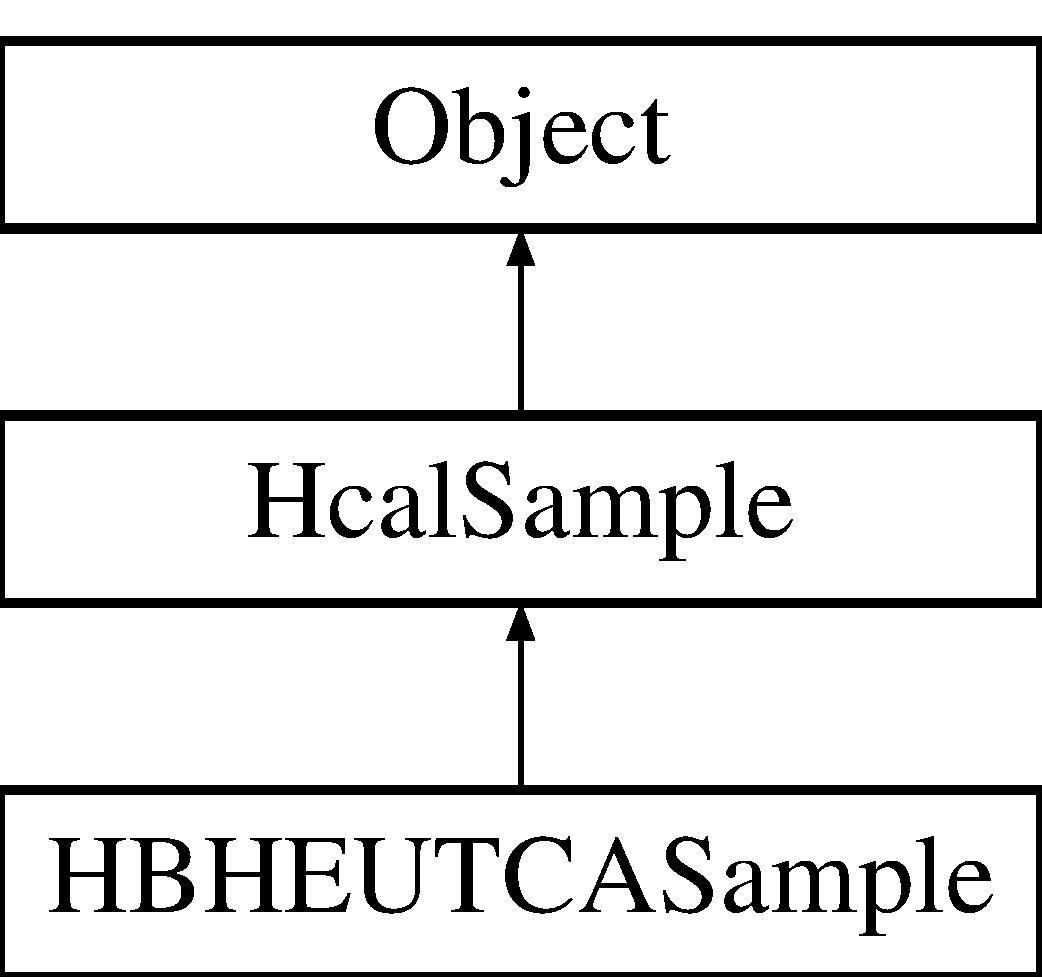
\includegraphics[height=3.000000cm]{class_h_b_h_e_u_t_c_a_sample}
\end{center}
\end{figure}
\subsection*{Public Member Functions}
\begin{DoxyCompactItemize}
\item 
\hyperlink{class_h_b_h_e_u_t_c_a_sample_ae1365988bbcbe0fb5e26888abde916a8}{H\+B\+H\+E\+U\+T\+C\+A\+Sample} ()
\item 
\hyperlink{class_h_b_h_e_u_t_c_a_sample_a8bb55e8750ed42f091ef603940be01dd}{H\+B\+H\+E\+U\+T\+C\+A\+Sample} (\hyperlink{class_collection}{Collection} \&c, unsigned short i, short j)
\item 
float \hyperlink{class_h_b_h_e_u_t_c_a_sample_adc02ae534bdfa6b4deee50da12fc638d}{all\+F\+C} ()
\item 
float \hyperlink{class_h_b_h_e_u_t_c_a_sample_a16cce3e525f59c9d92dc08fb9b685852}{energy} ()
\item 
float \hyperlink{class_h_b_h_e_u_t_c_a_sample_a5c7b26e64ac924f511411024b87cb669}{gain} ()
\item 
float \hyperlink{class_h_b_h_e_u_t_c_a_sample_a5792dd730d0c9051db9c4ef9dae69c32}{fc} ()
\item 
float \hyperlink{class_h_b_h_e_u_t_c_a_sample_ae261168bd8c528c76f8ef7ded47651a6}{nom\+F\+C} ()
\item 
float \hyperlink{class_h_b_h_e_u_t_c_a_sample_a0dc80ef00077e32025a6db5fc8d3fe3b}{ped\+F\+C} ()
\item 
float \hyperlink{class_h_b_h_e_u_t_c_a_sample_a7817d78373bf3a36594ebb581a08fb4c}{rc\+Gain} ()
\item 
int \hyperlink{class_h_b_h_e_u_t_c_a_sample_a9590d80a50ee9679e283bcc1d0896ea1}{adc} ()
\item 
int \hyperlink{class_h_b_h_e_u_t_c_a_sample_aa3428923215b84025833f1f558b70993}{capid} ()
\item 
int \hyperlink{class_h_b_h_e_u_t_c_a_sample_a804ca3a58ef7f4500639fdd22622e9dd}{dv} ()
\item 
int \hyperlink{class_h_b_h_e_u_t_c_a_sample_a02c629e33022099b919fba9e69b15054}{er} ()
\item 
int \hyperlink{class_h_b_h_e_u_t_c_a_sample_a99f62813e4808dfead59ab54846ec54a}{fiber} ()
\item 
int \hyperlink{class_h_b_h_e_u_t_c_a_sample_a5f57f71833cd7650af5361b4cb2a22e2}{fiber\+Chan} ()
\item 
int \hyperlink{class_h_b_h_e_u_t_c_a_sample_aa6673645bd8dec6413065dd5d426b0b8}{raw} ()
\item 
int \hyperlink{class_h_b_h_e_u_t_c_a_sample_ac08d2b48adfec0e67cea25c3db8586d5}{get\+Raw\+Index} ()
\item 
int \hyperlink{class_h_b_h_e_u_t_c_a_sample_a4080f843b5210360e0f6aacedc26b40a}{get\+Time\+Slice} ()
\end{DoxyCompactItemize}
\subsection*{Additional Inherited Members}


\subsection{Constructor \& Destructor Documentation}
\hypertarget{class_h_b_h_e_u_t_c_a_sample_ae1365988bbcbe0fb5e26888abde916a8}{}\index{H\+B\+H\+E\+U\+T\+C\+A\+Sample@{H\+B\+H\+E\+U\+T\+C\+A\+Sample}!H\+B\+H\+E\+U\+T\+C\+A\+Sample@{H\+B\+H\+E\+U\+T\+C\+A\+Sample}}
\index{H\+B\+H\+E\+U\+T\+C\+A\+Sample@{H\+B\+H\+E\+U\+T\+C\+A\+Sample}!H\+B\+H\+E\+U\+T\+C\+A\+Sample@{H\+B\+H\+E\+U\+T\+C\+A\+Sample}}
\subsubsection[{H\+B\+H\+E\+U\+T\+C\+A\+Sample()}]{\setlength{\rightskip}{0pt plus 5cm}H\+B\+H\+E\+U\+T\+C\+A\+Sample\+::\+H\+B\+H\+E\+U\+T\+C\+A\+Sample (
\begin{DoxyParamCaption}
{}
\end{DoxyParamCaption}
)}\label{class_h_b_h_e_u_t_c_a_sample_ae1365988bbcbe0fb5e26888abde916a8}
\hypertarget{class_h_b_h_e_u_t_c_a_sample_a8bb55e8750ed42f091ef603940be01dd}{}\index{H\+B\+H\+E\+U\+T\+C\+A\+Sample@{H\+B\+H\+E\+U\+T\+C\+A\+Sample}!H\+B\+H\+E\+U\+T\+C\+A\+Sample@{H\+B\+H\+E\+U\+T\+C\+A\+Sample}}
\index{H\+B\+H\+E\+U\+T\+C\+A\+Sample@{H\+B\+H\+E\+U\+T\+C\+A\+Sample}!H\+B\+H\+E\+U\+T\+C\+A\+Sample@{H\+B\+H\+E\+U\+T\+C\+A\+Sample}}
\subsubsection[{H\+B\+H\+E\+U\+T\+C\+A\+Sample(\+Collection \&c, unsigned short i, short j)}]{\setlength{\rightskip}{0pt plus 5cm}H\+B\+H\+E\+U\+T\+C\+A\+Sample\+::\+H\+B\+H\+E\+U\+T\+C\+A\+Sample (
\begin{DoxyParamCaption}
\item[{{\bf Collection} \&}]{c, }
\item[{unsigned short}]{i, }
\item[{short}]{j}
\end{DoxyParamCaption}
)}\label{class_h_b_h_e_u_t_c_a_sample_a8bb55e8750ed42f091ef603940be01dd}


\subsection{Member Function Documentation}
\hypertarget{class_h_b_h_e_u_t_c_a_sample_a9590d80a50ee9679e283bcc1d0896ea1}{}\index{H\+B\+H\+E\+U\+T\+C\+A\+Sample@{H\+B\+H\+E\+U\+T\+C\+A\+Sample}!adc@{adc}}
\index{adc@{adc}!H\+B\+H\+E\+U\+T\+C\+A\+Sample@{H\+B\+H\+E\+U\+T\+C\+A\+Sample}}
\subsubsection[{adc()}]{\setlength{\rightskip}{0pt plus 5cm}int H\+B\+H\+E\+U\+T\+C\+A\+Sample\+::adc (
\begin{DoxyParamCaption}
{}
\end{DoxyParamCaption}
)\hspace{0.3cm}{\ttfamily [virtual]}}\label{class_h_b_h_e_u_t_c_a_sample_a9590d80a50ee9679e283bcc1d0896ea1}


Implements \hyperlink{class_hcal_sample_a3801777ac080ca0e512c226e4cfd5682}{Hcal\+Sample}.

\hypertarget{class_h_b_h_e_u_t_c_a_sample_adc02ae534bdfa6b4deee50da12fc638d}{}\index{H\+B\+H\+E\+U\+T\+C\+A\+Sample@{H\+B\+H\+E\+U\+T\+C\+A\+Sample}!all\+F\+C@{all\+F\+C}}
\index{all\+F\+C@{all\+F\+C}!H\+B\+H\+E\+U\+T\+C\+A\+Sample@{H\+B\+H\+E\+U\+T\+C\+A\+Sample}}
\subsubsection[{all\+F\+C()}]{\setlength{\rightskip}{0pt plus 5cm}float H\+B\+H\+E\+U\+T\+C\+A\+Sample\+::all\+F\+C (
\begin{DoxyParamCaption}
{}
\end{DoxyParamCaption}
)\hspace{0.3cm}{\ttfamily [virtual]}}\label{class_h_b_h_e_u_t_c_a_sample_adc02ae534bdfa6b4deee50da12fc638d}


Implements \hyperlink{class_hcal_sample_af837bd894eb8eae865023a526940ee15}{Hcal\+Sample}.

\hypertarget{class_h_b_h_e_u_t_c_a_sample_aa3428923215b84025833f1f558b70993}{}\index{H\+B\+H\+E\+U\+T\+C\+A\+Sample@{H\+B\+H\+E\+U\+T\+C\+A\+Sample}!capid@{capid}}
\index{capid@{capid}!H\+B\+H\+E\+U\+T\+C\+A\+Sample@{H\+B\+H\+E\+U\+T\+C\+A\+Sample}}
\subsubsection[{capid()}]{\setlength{\rightskip}{0pt plus 5cm}int H\+B\+H\+E\+U\+T\+C\+A\+Sample\+::capid (
\begin{DoxyParamCaption}
{}
\end{DoxyParamCaption}
)\hspace{0.3cm}{\ttfamily [virtual]}}\label{class_h_b_h_e_u_t_c_a_sample_aa3428923215b84025833f1f558b70993}


Implements \hyperlink{class_hcal_sample_a51a82042ba140a68f9659140c48d83bc}{Hcal\+Sample}.

\hypertarget{class_h_b_h_e_u_t_c_a_sample_a804ca3a58ef7f4500639fdd22622e9dd}{}\index{H\+B\+H\+E\+U\+T\+C\+A\+Sample@{H\+B\+H\+E\+U\+T\+C\+A\+Sample}!dv@{dv}}
\index{dv@{dv}!H\+B\+H\+E\+U\+T\+C\+A\+Sample@{H\+B\+H\+E\+U\+T\+C\+A\+Sample}}
\subsubsection[{dv()}]{\setlength{\rightskip}{0pt plus 5cm}int H\+B\+H\+E\+U\+T\+C\+A\+Sample\+::dv (
\begin{DoxyParamCaption}
{}
\end{DoxyParamCaption}
)\hspace{0.3cm}{\ttfamily [virtual]}}\label{class_h_b_h_e_u_t_c_a_sample_a804ca3a58ef7f4500639fdd22622e9dd}


Implements \hyperlink{class_hcal_sample_a13c0e851a42d3122c7bba32d81e31d19}{Hcal\+Sample}.

\hypertarget{class_h_b_h_e_u_t_c_a_sample_a16cce3e525f59c9d92dc08fb9b685852}{}\index{H\+B\+H\+E\+U\+T\+C\+A\+Sample@{H\+B\+H\+E\+U\+T\+C\+A\+Sample}!energy@{energy}}
\index{energy@{energy}!H\+B\+H\+E\+U\+T\+C\+A\+Sample@{H\+B\+H\+E\+U\+T\+C\+A\+Sample}}
\subsubsection[{energy()}]{\setlength{\rightskip}{0pt plus 5cm}float H\+B\+H\+E\+U\+T\+C\+A\+Sample\+::energy (
\begin{DoxyParamCaption}
{}
\end{DoxyParamCaption}
)\hspace{0.3cm}{\ttfamily [virtual]}}\label{class_h_b_h_e_u_t_c_a_sample_a16cce3e525f59c9d92dc08fb9b685852}


Implements \hyperlink{class_hcal_sample_a603c4e95d1d49db37dd00f34275fb8f3}{Hcal\+Sample}.

\hypertarget{class_h_b_h_e_u_t_c_a_sample_a02c629e33022099b919fba9e69b15054}{}\index{H\+B\+H\+E\+U\+T\+C\+A\+Sample@{H\+B\+H\+E\+U\+T\+C\+A\+Sample}!er@{er}}
\index{er@{er}!H\+B\+H\+E\+U\+T\+C\+A\+Sample@{H\+B\+H\+E\+U\+T\+C\+A\+Sample}}
\subsubsection[{er()}]{\setlength{\rightskip}{0pt plus 5cm}int H\+B\+H\+E\+U\+T\+C\+A\+Sample\+::er (
\begin{DoxyParamCaption}
{}
\end{DoxyParamCaption}
)\hspace{0.3cm}{\ttfamily [virtual]}}\label{class_h_b_h_e_u_t_c_a_sample_a02c629e33022099b919fba9e69b15054}


Implements \hyperlink{class_hcal_sample_af1805d239ccbc17a6c307d66522da618}{Hcal\+Sample}.

\hypertarget{class_h_b_h_e_u_t_c_a_sample_a5792dd730d0c9051db9c4ef9dae69c32}{}\index{H\+B\+H\+E\+U\+T\+C\+A\+Sample@{H\+B\+H\+E\+U\+T\+C\+A\+Sample}!fc@{fc}}
\index{fc@{fc}!H\+B\+H\+E\+U\+T\+C\+A\+Sample@{H\+B\+H\+E\+U\+T\+C\+A\+Sample}}
\subsubsection[{fc()}]{\setlength{\rightskip}{0pt plus 5cm}float H\+B\+H\+E\+U\+T\+C\+A\+Sample\+::fc (
\begin{DoxyParamCaption}
{}
\end{DoxyParamCaption}
)\hspace{0.3cm}{\ttfamily [virtual]}}\label{class_h_b_h_e_u_t_c_a_sample_a5792dd730d0c9051db9c4ef9dae69c32}


Implements \hyperlink{class_hcal_sample_aed932c9f932eabed9f9bc6b1a54c20dd}{Hcal\+Sample}.

\hypertarget{class_h_b_h_e_u_t_c_a_sample_a99f62813e4808dfead59ab54846ec54a}{}\index{H\+B\+H\+E\+U\+T\+C\+A\+Sample@{H\+B\+H\+E\+U\+T\+C\+A\+Sample}!fiber@{fiber}}
\index{fiber@{fiber}!H\+B\+H\+E\+U\+T\+C\+A\+Sample@{H\+B\+H\+E\+U\+T\+C\+A\+Sample}}
\subsubsection[{fiber()}]{\setlength{\rightskip}{0pt plus 5cm}int H\+B\+H\+E\+U\+T\+C\+A\+Sample\+::fiber (
\begin{DoxyParamCaption}
{}
\end{DoxyParamCaption}
)\hspace{0.3cm}{\ttfamily [virtual]}}\label{class_h_b_h_e_u_t_c_a_sample_a99f62813e4808dfead59ab54846ec54a}


Implements \hyperlink{class_hcal_sample_a5ae9a4d213b69f5ee382c7a6b31eb446}{Hcal\+Sample}.

\hypertarget{class_h_b_h_e_u_t_c_a_sample_a5f57f71833cd7650af5361b4cb2a22e2}{}\index{H\+B\+H\+E\+U\+T\+C\+A\+Sample@{H\+B\+H\+E\+U\+T\+C\+A\+Sample}!fiber\+Chan@{fiber\+Chan}}
\index{fiber\+Chan@{fiber\+Chan}!H\+B\+H\+E\+U\+T\+C\+A\+Sample@{H\+B\+H\+E\+U\+T\+C\+A\+Sample}}
\subsubsection[{fiber\+Chan()}]{\setlength{\rightskip}{0pt plus 5cm}int H\+B\+H\+E\+U\+T\+C\+A\+Sample\+::fiber\+Chan (
\begin{DoxyParamCaption}
{}
\end{DoxyParamCaption}
)\hspace{0.3cm}{\ttfamily [virtual]}}\label{class_h_b_h_e_u_t_c_a_sample_a5f57f71833cd7650af5361b4cb2a22e2}


Implements \hyperlink{class_hcal_sample_acdd36acaedfe4e1a6114e6c56d1ed996}{Hcal\+Sample}.

\hypertarget{class_h_b_h_e_u_t_c_a_sample_a5c7b26e64ac924f511411024b87cb669}{}\index{H\+B\+H\+E\+U\+T\+C\+A\+Sample@{H\+B\+H\+E\+U\+T\+C\+A\+Sample}!gain@{gain}}
\index{gain@{gain}!H\+B\+H\+E\+U\+T\+C\+A\+Sample@{H\+B\+H\+E\+U\+T\+C\+A\+Sample}}
\subsubsection[{gain()}]{\setlength{\rightskip}{0pt plus 5cm}float H\+B\+H\+E\+U\+T\+C\+A\+Sample\+::gain (
\begin{DoxyParamCaption}
{}
\end{DoxyParamCaption}
)\hspace{0.3cm}{\ttfamily [virtual]}}\label{class_h_b_h_e_u_t_c_a_sample_a5c7b26e64ac924f511411024b87cb669}


Implements \hyperlink{class_hcal_sample_aefc3dd058b3b178917583ca6abbf4f01}{Hcal\+Sample}.

\hypertarget{class_h_b_h_e_u_t_c_a_sample_ac08d2b48adfec0e67cea25c3db8586d5}{}\index{H\+B\+H\+E\+U\+T\+C\+A\+Sample@{H\+B\+H\+E\+U\+T\+C\+A\+Sample}!get\+Raw\+Index@{get\+Raw\+Index}}
\index{get\+Raw\+Index@{get\+Raw\+Index}!H\+B\+H\+E\+U\+T\+C\+A\+Sample@{H\+B\+H\+E\+U\+T\+C\+A\+Sample}}
\subsubsection[{get\+Raw\+Index()}]{\setlength{\rightskip}{0pt plus 5cm}int H\+B\+H\+E\+U\+T\+C\+A\+Sample\+::get\+Raw\+Index (
\begin{DoxyParamCaption}
{}
\end{DoxyParamCaption}
)\hspace{0.3cm}{\ttfamily [inline]}}\label{class_h_b_h_e_u_t_c_a_sample_ac08d2b48adfec0e67cea25c3db8586d5}
\hypertarget{class_h_b_h_e_u_t_c_a_sample_a4080f843b5210360e0f6aacedc26b40a}{}\index{H\+B\+H\+E\+U\+T\+C\+A\+Sample@{H\+B\+H\+E\+U\+T\+C\+A\+Sample}!get\+Time\+Slice@{get\+Time\+Slice}}
\index{get\+Time\+Slice@{get\+Time\+Slice}!H\+B\+H\+E\+U\+T\+C\+A\+Sample@{H\+B\+H\+E\+U\+T\+C\+A\+Sample}}
\subsubsection[{get\+Time\+Slice()}]{\setlength{\rightskip}{0pt plus 5cm}int H\+B\+H\+E\+U\+T\+C\+A\+Sample\+::get\+Time\+Slice (
\begin{DoxyParamCaption}
{}
\end{DoxyParamCaption}
)\hspace{0.3cm}{\ttfamily [inline]}}\label{class_h_b_h_e_u_t_c_a_sample_a4080f843b5210360e0f6aacedc26b40a}
\hypertarget{class_h_b_h_e_u_t_c_a_sample_ae261168bd8c528c76f8ef7ded47651a6}{}\index{H\+B\+H\+E\+U\+T\+C\+A\+Sample@{H\+B\+H\+E\+U\+T\+C\+A\+Sample}!nom\+F\+C@{nom\+F\+C}}
\index{nom\+F\+C@{nom\+F\+C}!H\+B\+H\+E\+U\+T\+C\+A\+Sample@{H\+B\+H\+E\+U\+T\+C\+A\+Sample}}
\subsubsection[{nom\+F\+C()}]{\setlength{\rightskip}{0pt plus 5cm}float H\+B\+H\+E\+U\+T\+C\+A\+Sample\+::nom\+F\+C (
\begin{DoxyParamCaption}
{}
\end{DoxyParamCaption}
)\hspace{0.3cm}{\ttfamily [virtual]}}\label{class_h_b_h_e_u_t_c_a_sample_ae261168bd8c528c76f8ef7ded47651a6}


Implements \hyperlink{class_hcal_sample_a9f47a5b867c94c97c3d553e244e7dc87}{Hcal\+Sample}.

\hypertarget{class_h_b_h_e_u_t_c_a_sample_a0dc80ef00077e32025a6db5fc8d3fe3b}{}\index{H\+B\+H\+E\+U\+T\+C\+A\+Sample@{H\+B\+H\+E\+U\+T\+C\+A\+Sample}!ped\+F\+C@{ped\+F\+C}}
\index{ped\+F\+C@{ped\+F\+C}!H\+B\+H\+E\+U\+T\+C\+A\+Sample@{H\+B\+H\+E\+U\+T\+C\+A\+Sample}}
\subsubsection[{ped\+F\+C()}]{\setlength{\rightskip}{0pt plus 5cm}float H\+B\+H\+E\+U\+T\+C\+A\+Sample\+::ped\+F\+C (
\begin{DoxyParamCaption}
{}
\end{DoxyParamCaption}
)\hspace{0.3cm}{\ttfamily [virtual]}}\label{class_h_b_h_e_u_t_c_a_sample_a0dc80ef00077e32025a6db5fc8d3fe3b}


Implements \hyperlink{class_hcal_sample_a471f7ef87944ac870ea884a0cc957744}{Hcal\+Sample}.

\hypertarget{class_h_b_h_e_u_t_c_a_sample_aa6673645bd8dec6413065dd5d426b0b8}{}\index{H\+B\+H\+E\+U\+T\+C\+A\+Sample@{H\+B\+H\+E\+U\+T\+C\+A\+Sample}!raw@{raw}}
\index{raw@{raw}!H\+B\+H\+E\+U\+T\+C\+A\+Sample@{H\+B\+H\+E\+U\+T\+C\+A\+Sample}}
\subsubsection[{raw()}]{\setlength{\rightskip}{0pt plus 5cm}int H\+B\+H\+E\+U\+T\+C\+A\+Sample\+::raw (
\begin{DoxyParamCaption}
{}
\end{DoxyParamCaption}
)\hspace{0.3cm}{\ttfamily [virtual]}}\label{class_h_b_h_e_u_t_c_a_sample_aa6673645bd8dec6413065dd5d426b0b8}


Implements \hyperlink{class_hcal_sample_a328a0f8f80a0aae47a92500297635bd6}{Hcal\+Sample}.

\hypertarget{class_h_b_h_e_u_t_c_a_sample_a7817d78373bf3a36594ebb581a08fb4c}{}\index{H\+B\+H\+E\+U\+T\+C\+A\+Sample@{H\+B\+H\+E\+U\+T\+C\+A\+Sample}!rc\+Gain@{rc\+Gain}}
\index{rc\+Gain@{rc\+Gain}!H\+B\+H\+E\+U\+T\+C\+A\+Sample@{H\+B\+H\+E\+U\+T\+C\+A\+Sample}}
\subsubsection[{rc\+Gain()}]{\setlength{\rightskip}{0pt plus 5cm}float H\+B\+H\+E\+U\+T\+C\+A\+Sample\+::rc\+Gain (
\begin{DoxyParamCaption}
{}
\end{DoxyParamCaption}
)\hspace{0.3cm}{\ttfamily [virtual]}}\label{class_h_b_h_e_u_t_c_a_sample_a7817d78373bf3a36594ebb581a08fb4c}


Implements \hyperlink{class_hcal_sample_a6fd32da2d5ea80154251de366f98c49c}{Hcal\+Sample}.



The documentation for this class was generated from the following file\+:\begin{DoxyCompactItemize}
\item 
interface/\hyperlink{_h_b_h_e_u_t_c_a_sample_8h}{H\+B\+H\+E\+U\+T\+C\+A\+Sample.\+h}\end{DoxyCompactItemize}

\hypertarget{class_hcal_data}{}\section{Hcal\+Data Class Reference}
\label{class_hcal_data}\index{Hcal\+Data@{Hcal\+Data}}


Class for exposing H\+C\+A\+L data from \hyperlink{class_hcal_tuple_tree}{Hcal\+Tuple\+Tree} (github.\+com/\+H\+C\+A\+L\+P\+F\+G/\+Hcal\+Tuple\+Maker) in pyroot. Digi data is available through the various Digi objects. Data can also be directly accessed in the usual T\+Tree\+::\+Make\+Selector way.  




{\ttfamily \#include $<$Hcal\+Data.\+h$>$}

Inheritance diagram for Hcal\+Data\+:\begin{figure}[H]
\begin{center}
\leavevmode
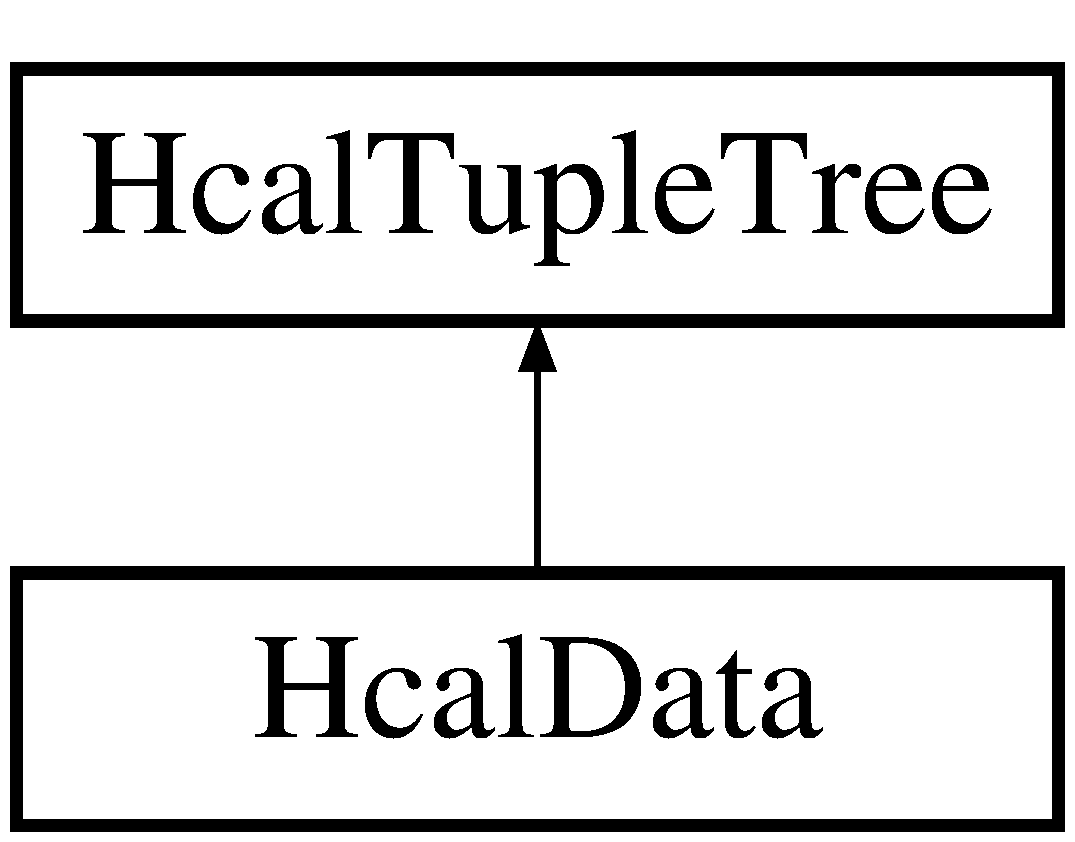
\includegraphics[height=2.000000cm]{class_hcal_data}
\end{center}
\end{figure}
\subsection*{Public Member Functions}
\begin{DoxyCompactItemize}
\item 
\hyperlink{class_hcal_data_a03e8c0684f3121d68944cd71d0c02817}{Hcal\+Data} (T\+Tree $\ast$tree=0)
\item 
\hyperlink{class_hcal_data_a6a6311896ad7d9aa300f01572cf2c9f5}{$\sim$\+Hcal\+Data} ()
\item 
Int\+\_\+t \hyperlink{class_hcal_data_aa5d32f6b744c860c647e213d4aff9ff4}{Get\+Entry} (Long64\+\_\+t entry)
\item 
{\footnotesize template$<$class T $>$ }\\\hyperlink{class_collection}{Collection} $\ast$ \hyperlink{class_hcal_data_a620712e779255411ccd8aedf375f430d}{Digis} ()
\begin{DoxyCompactList}\small\item\em Returns a collection of digis based on the template class (\hyperlink{class_h_b_h_e_digi}{H\+B\+H\+E\+Digi}, \hyperlink{class_h_f_digi}{H\+F\+Digi}, or \hyperlink{class_h_o_digi}{H\+O\+Digi}). \end{DoxyCompactList}\item 
{\footnotesize template$<$class T $>$ }\\T \hyperlink{class_hcal_data_a36161d851fde7fb81c4d1b616ff09680}{Digi} (int i)
\begin{DoxyCompactList}\small\item\em Returns a single digi. Type is determined from the template class. \end{DoxyCompactList}\item 
void \hyperlink{class_hcal_data_ac2257a06065a51a4c23d4007beb8ad64}{Add\+Detector} (\hyperlink{namespacepfg_a90b6d47b5ff56bc3ebabb0f6b6088d60}{pfg\+::\+Detector\+\_\+t} detector)
\begin{DoxyCompactList}\small\item\em Make a detector\textquotesingle{}s data available through \hyperlink{class_hcal_data_a36161d851fde7fb81c4d1b616ff09680}{Hcal\+Data\+::\+Digi} and \hyperlink{class_hcal_data_a620712e779255411ccd8aedf375f430d}{Hcal\+Data\+::\+Digis}. \end{DoxyCompactList}\end{DoxyCompactItemize}
\subsection*{Additional Inherited Members}


\subsection{Detailed Description}
Class for exposing H\+C\+A\+L data from \hyperlink{class_hcal_tuple_tree}{Hcal\+Tuple\+Tree} (github.\+com/\+H\+C\+A\+L\+P\+F\+G/\+Hcal\+Tuple\+Maker) in pyroot. Digi data is available through the various Digi objects. Data can also be directly accessed in the usual T\+Tree\+::\+Make\+Selector way. 

\subsection{Constructor \& Destructor Documentation}
\hypertarget{class_hcal_data_a03e8c0684f3121d68944cd71d0c02817}{}\index{Hcal\+Data@{Hcal\+Data}!Hcal\+Data@{Hcal\+Data}}
\index{Hcal\+Data@{Hcal\+Data}!Hcal\+Data@{Hcal\+Data}}
\subsubsection[{Hcal\+Data(\+T\+Tree $\ast$tree=0)}]{\setlength{\rightskip}{0pt plus 5cm}Hcal\+Data\+::\+Hcal\+Data (
\begin{DoxyParamCaption}
\item[{T\+Tree $\ast$}]{tree = {\ttfamily 0}}
\end{DoxyParamCaption}
)}\label{class_hcal_data_a03e8c0684f3121d68944cd71d0c02817}
\hypertarget{class_hcal_data_a6a6311896ad7d9aa300f01572cf2c9f5}{}\index{Hcal\+Data@{Hcal\+Data}!````~Hcal\+Data@{$\sim$\+Hcal\+Data}}
\index{````~Hcal\+Data@{$\sim$\+Hcal\+Data}!Hcal\+Data@{Hcal\+Data}}
\subsubsection[{$\sim$\+Hcal\+Data()}]{\setlength{\rightskip}{0pt plus 5cm}Hcal\+Data\+::$\sim$\+Hcal\+Data (
\begin{DoxyParamCaption}
{}
\end{DoxyParamCaption}
)}\label{class_hcal_data_a6a6311896ad7d9aa300f01572cf2c9f5}


\subsection{Member Function Documentation}
\hypertarget{class_hcal_data_ac2257a06065a51a4c23d4007beb8ad64}{}\index{Hcal\+Data@{Hcal\+Data}!Add\+Detector@{Add\+Detector}}
\index{Add\+Detector@{Add\+Detector}!Hcal\+Data@{Hcal\+Data}}
\subsubsection[{Add\+Detector(pfg\+::\+Detector\+\_\+t detector)}]{\setlength{\rightskip}{0pt plus 5cm}void Hcal\+Data\+::\+Add\+Detector (
\begin{DoxyParamCaption}
\item[{{\bf pfg\+::\+Detector\+\_\+t}}]{detector}
\end{DoxyParamCaption}
)\hspace{0.3cm}{\ttfamily [inline]}}\label{class_hcal_data_ac2257a06065a51a4c23d4007beb8ad64}


Make a detector\textquotesingle{}s data available through \hyperlink{class_hcal_data_a36161d851fde7fb81c4d1b616ff09680}{Hcal\+Data\+::\+Digi} and \hyperlink{class_hcal_data_a620712e779255411ccd8aedf375f430d}{Hcal\+Data\+::\+Digis}. 


\begin{DoxyParams}[1]{Parameters}
\mbox{\tt in}  & {\em detector} & \hyperlink{namespacepfg_a90b6d47b5ff56bc3ebabb0f6b6088d60a6dd4ec12d707ea8f3768d5ce35598ef7}{pfg\+::k\+H\+B\+H\+E}, \hyperlink{namespacepfg_a90b6d47b5ff56bc3ebabb0f6b6088d60af0455c45bb2be69b625695b04157afab}{pfg\+::k\+H\+F}, or \hyperlink{namespacepfg_a90b6d47b5ff56bc3ebabb0f6b6088d60a438afa76c58d2c9c8df4e1b8f90f4789}{pfg\+::k\+H\+O}. \\
\hline
\end{DoxyParams}
\hypertarget{class_hcal_data_a36161d851fde7fb81c4d1b616ff09680}{}\index{Hcal\+Data@{Hcal\+Data}!Digi@{Digi}}
\index{Digi@{Digi}!Hcal\+Data@{Hcal\+Data}}
\subsubsection[{Digi(int i)}]{\setlength{\rightskip}{0pt plus 5cm}template$<$class T $>$ T Hcal\+Data\+::\+Digi (
\begin{DoxyParamCaption}
\item[{int}]{i}
\end{DoxyParamCaption}
)\hspace{0.3cm}{\ttfamily [inline]}}\label{class_hcal_data_a36161d851fde7fb81c4d1b616ff09680}


Returns a single digi. Type is determined from the template class. 


\begin{DoxyParams}{Parameters}
{\em \mbox{[}int\mbox{]}} & i Index of digi \\
\hline
\end{DoxyParams}
\begin{DoxyReturn}{Returns}
Digi 
\end{DoxyReturn}
\hypertarget{class_hcal_data_a620712e779255411ccd8aedf375f430d}{}\index{Hcal\+Data@{Hcal\+Data}!Digis@{Digis}}
\index{Digis@{Digis}!Hcal\+Data@{Hcal\+Data}}
\subsubsection[{Digis()}]{\setlength{\rightskip}{0pt plus 5cm}template$<$class T $>$ {\bf Collection}$\ast$ Hcal\+Data\+::\+Digis (
\begin{DoxyParamCaption}
{}
\end{DoxyParamCaption}
)\hspace{0.3cm}{\ttfamily [inline]}}\label{class_hcal_data_a620712e779255411ccd8aedf375f430d}


Returns a collection of digis based on the template class (\hyperlink{class_h_b_h_e_digi}{H\+B\+H\+E\+Digi}, \hyperlink{class_h_f_digi}{H\+F\+Digi}, or \hyperlink{class_h_o_digi}{H\+O\+Digi}). 

\begin{DoxyReturn}{Returns}
\hyperlink{class_collection}{Collection} of digis. 
\end{DoxyReturn}
\hypertarget{class_hcal_data_aa5d32f6b744c860c647e213d4aff9ff4}{}\index{Hcal\+Data@{Hcal\+Data}!Get\+Entry@{Get\+Entry}}
\index{Get\+Entry@{Get\+Entry}!Hcal\+Data@{Hcal\+Data}}
\subsubsection[{Get\+Entry(\+Long64\+\_\+t entry)}]{\setlength{\rightskip}{0pt plus 5cm}Int\+\_\+t Hcal\+Data\+::\+Get\+Entry (
\begin{DoxyParamCaption}
\item[{Long64\+\_\+t}]{entry}
\end{DoxyParamCaption}
)\hspace{0.3cm}{\ttfamily [virtual]}}\label{class_hcal_data_aa5d32f6b744c860c647e213d4aff9ff4}


Reimplemented from \hyperlink{class_hcal_tuple_tree_a61ac2553042cf88a12bd462a7814c18d}{Hcal\+Tuple\+Tree}.



The documentation for this class was generated from the following files\+:\begin{DoxyCompactItemize}
\item 
interface/\hyperlink{_hcal_data_8h}{Hcal\+Data.\+h}\item 
src/\hyperlink{_hcal_data_8cc}{Hcal\+Data.\+cc}\end{DoxyCompactItemize}

\hypertarget{class_hcal_digi}{}\section{Hcal\+Digi Class Reference}
\label{class_hcal_digi}\index{Hcal\+Digi@{Hcal\+Digi}}


{\ttfamily \#include $<$Hcal\+Digi.\+h$>$}

Inheritance diagram for Hcal\+Digi\+:\begin{figure}[H]
\begin{center}
\leavevmode
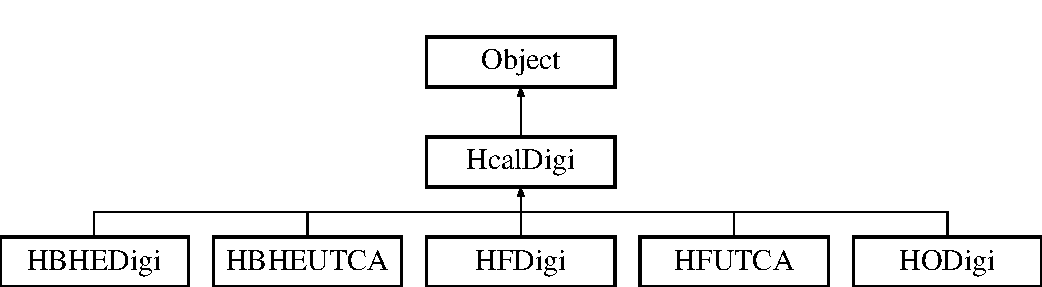
\includegraphics[height=3.000000cm]{class_hcal_digi}
\end{center}
\end{figure}
\subsection*{Public Member Functions}
\begin{DoxyCompactItemize}
\item 
\hyperlink{class_hcal_digi_a0577e9f390ff911e083f7465cb0e8f1d}{Hcal\+Digi} ()
\item 
\hyperlink{class_hcal_digi_a5f4c54b1683c340b0256aa35efb951ca}{Hcal\+Digi} (\hyperlink{class_collection}{Collection} \&c, unsigned short i, short j=0)
\item 
virtual float \hyperlink{class_hcal_digi_a665c0fa940132fafc6dce9fd75f18cea}{energy} ()=0
\item 
virtual float \hyperlink{class_hcal_digi_a3936cda623fc7535ed35d8d1c6abb350}{rec\+Hit\+Time} ()=0
\item 
virtual int \hyperlink{class_hcal_digi_a65fc605c5c3bca7f78d961400d145c94}{ieta} ()=0
\item 
virtual int \hyperlink{class_hcal_digi_a979dec4585c9d07a7dc4060dfb97f089}{iphi} ()=0
\item 
virtual int \hyperlink{class_hcal_digi_a916a582b044a64e041ba38e545349f7f}{depth} ()=0
\item 
virtual int \hyperlink{class_hcal_digi_a054f6f17539c8042d2900144d06eb4fc}{size} ()=0
\item 
virtual int \hyperlink{class_hcal_digi_aad0fc232379d8bdd40d6be32b3c980c4}{presamples} ()=0
\item 
virtual int \hyperlink{class_hcal_digi_afc95a09767a731b098cb2e22b89cc4e0}{electronics\+Id} ()=0
\item 
virtual int \hyperlink{class_hcal_digi_aba55732d16499ad510091c769807f8e1}{raw\+Id} ()=0
\item 
virtual float \hyperlink{class_hcal_digi_a4a5e45ca390ee81fe384bf4a7d05f1e0}{fc} (int i)=0
\item 
virtual int \hyperlink{class_hcal_digi_a737b46ab9bc5439f32232ee6911ed516}{adc} (int i)=0
\item 
virtual int \hyperlink{class_hcal_digi_aa758519b70ab24ac4bb7635052cfa174}{dv} (int i)=0
\item 
virtual int \hyperlink{class_hcal_digi_a04b02a86692bcdff2fb8fa8c50cc0c34}{er} (int i)=0
\item 
virtual int \hyperlink{class_hcal_digi_ad6e205312dda117af660b9391d502155}{capid} (int i)=0
\item 
float \hyperlink{class_hcal_digi_a138d4ee8f433530dd2ed391cf036f233}{fc\+Total} ()
\item 
int \hyperlink{class_hcal_digi_a24ca24cbc2ea356627ddcff20c308846}{adc\+Total} ()
\item 
double \hyperlink{class_hcal_digi_a11e29234e593020716fea46884cdb850}{time} ()
\item 
double \hyperlink{class_hcal_digi_a9d7d21b996bfffcac0543d43d167c5ea}{time12} ()
\item 
double \hyperlink{class_hcal_digi_a298c1a07be693c4b7eb575ff73986d3a}{time34} ()
\item 
double \hyperlink{class_hcal_digi_ab6a0cbf1a35a0fb01eb91e8cd90f4cb2}{charge12} ()
\item 
double \hyperlink{class_hcal_digi_aee6d8c5093f2a13ea727f9582893bfa0}{charge34} ()
\item 
bool \hyperlink{class_hcal_digi_a533e89804901926f571c8bf5ab3a28d9}{is\+Signal} ()
\item 
int \hyperlink{class_hcal_digi_a1b0ece60d015d716a91cde135caefb34}{max\+A\+D\+C} ()
\item 
double \& \hyperlink{class_hcal_digi_a97f21992c1e45b427ce09dcca581e0f5}{Pt} ()
\item 
double \& \hyperlink{class_hcal_digi_a84be4fe4f387b7b67da4161b70e6254a}{Eta} ()
\item 
double \& \hyperlink{class_hcal_digi_a3cc5e61af592f544a573f2bd8d0292f7}{Phi} ()
\item 
bool \hyperlink{class_hcal_digi_aff5580b98a1dc9155ee316ea30c52701}{Pass\+User\+I\+D} (\hyperlink{_i_d_types_8h_a094c367727273b4da2b960ca3b3edc06}{I\+D} id, bool verbose=false)
\item 
bool \hyperlink{class_hcal_digi_ad46ecbe02799bfd4f955d16d6cc8a634}{Pass\+User\+I\+D\+\_\+\+Digi\+Has\+N\+D\+V} (bool verbose)
\item 
bool \hyperlink{class_hcal_digi_a37f77ef16bee597453274322be29b9d3}{Pass\+User\+I\+D\+\_\+\+Digi\+Has\+E\+R} (bool verbose)
\item 
bool \hyperlink{class_hcal_digi_ad67d910037f433d03888ab45d12cbe1b}{Pass\+User\+I\+D\+\_\+\+Digi\+Has\+Cap\+I\+D\+Err} (bool verbose)
\item 
bool \hyperlink{class_hcal_digi_a2a05f5e8ab79e930d4eb421c4569d374}{Pass\+User\+I\+D\+\_\+\+Digi\+Has\+Bad\+Size} (bool verbose)
\item 
bool \hyperlink{class_hcal_digi_a515c743373f90bdfe0a43297cb7e957b}{Pass\+User\+I\+D\+\_\+\+Digi\+Is\+Signal} (bool verbose)
\end{DoxyCompactItemize}
\subsection*{Protected Attributes}
\begin{DoxyCompactItemize}
\item 
double \hyperlink{class_hcal_digi_a4829a0f328a240dd236569a3cf717c4f}{m\+\_\+null\+\_\+value}
\end{DoxyCompactItemize}


\subsection{Constructor \& Destructor Documentation}
\hypertarget{class_hcal_digi_a0577e9f390ff911e083f7465cb0e8f1d}{}\index{Hcal\+Digi@{Hcal\+Digi}!Hcal\+Digi@{Hcal\+Digi}}
\index{Hcal\+Digi@{Hcal\+Digi}!Hcal\+Digi@{Hcal\+Digi}}
\subsubsection[{Hcal\+Digi()}]{\setlength{\rightskip}{0pt plus 5cm}Hcal\+Digi\+::\+Hcal\+Digi (
\begin{DoxyParamCaption}
{}
\end{DoxyParamCaption}
)}\label{class_hcal_digi_a0577e9f390ff911e083f7465cb0e8f1d}
\hypertarget{class_hcal_digi_a5f4c54b1683c340b0256aa35efb951ca}{}\index{Hcal\+Digi@{Hcal\+Digi}!Hcal\+Digi@{Hcal\+Digi}}
\index{Hcal\+Digi@{Hcal\+Digi}!Hcal\+Digi@{Hcal\+Digi}}
\subsubsection[{Hcal\+Digi(\+Collection \&c, unsigned short i, short j=0)}]{\setlength{\rightskip}{0pt plus 5cm}Hcal\+Digi\+::\+Hcal\+Digi (
\begin{DoxyParamCaption}
\item[{{\bf Collection} \&}]{c, }
\item[{unsigned short}]{i, }
\item[{short}]{j = {\ttfamily 0}}
\end{DoxyParamCaption}
)}\label{class_hcal_digi_a5f4c54b1683c340b0256aa35efb951ca}


\subsection{Member Function Documentation}
\hypertarget{class_hcal_digi_a737b46ab9bc5439f32232ee6911ed516}{}\index{Hcal\+Digi@{Hcal\+Digi}!adc@{adc}}
\index{adc@{adc}!Hcal\+Digi@{Hcal\+Digi}}
\subsubsection[{adc(int i)=0}]{\setlength{\rightskip}{0pt plus 5cm}virtual int Hcal\+Digi\+::adc (
\begin{DoxyParamCaption}
\item[{int}]{i}
\end{DoxyParamCaption}
)\hspace{0.3cm}{\ttfamily [pure virtual]}}\label{class_hcal_digi_a737b46ab9bc5439f32232ee6911ed516}


Implemented in \hyperlink{class_h_b_h_e_digi_a13245b123aa2a7b9a77783ef063a2e9e}{H\+B\+H\+E\+Digi}, \hyperlink{class_h_b_h_e_u_t_c_a_abeffd6ef4e4023b16b3e34b4ee08946a}{H\+B\+H\+E\+U\+T\+C\+A}, \hyperlink{class_h_f_digi_afd736e6e2a6292cd2e88cac49b7e919d}{H\+F\+Digi}, \hyperlink{class_h_f_u_t_c_a_ad7540b3f782bf6fecc3d00ffd8432337}{H\+F\+U\+T\+C\+A}, and \hyperlink{class_h_o_digi_a3e6b23ebca7eb32e5bc88176714e70c0}{H\+O\+Digi}.

\hypertarget{class_hcal_digi_a24ca24cbc2ea356627ddcff20c308846}{}\index{Hcal\+Digi@{Hcal\+Digi}!adc\+Total@{adc\+Total}}
\index{adc\+Total@{adc\+Total}!Hcal\+Digi@{Hcal\+Digi}}
\subsubsection[{adc\+Total()}]{\setlength{\rightskip}{0pt plus 5cm}int Hcal\+Digi\+::adc\+Total (
\begin{DoxyParamCaption}
{}
\end{DoxyParamCaption}
)}\label{class_hcal_digi_a24ca24cbc2ea356627ddcff20c308846}
\hypertarget{class_hcal_digi_ad6e205312dda117af660b9391d502155}{}\index{Hcal\+Digi@{Hcal\+Digi}!capid@{capid}}
\index{capid@{capid}!Hcal\+Digi@{Hcal\+Digi}}
\subsubsection[{capid(int i)=0}]{\setlength{\rightskip}{0pt plus 5cm}virtual int Hcal\+Digi\+::capid (
\begin{DoxyParamCaption}
\item[{int}]{i}
\end{DoxyParamCaption}
)\hspace{0.3cm}{\ttfamily [pure virtual]}}\label{class_hcal_digi_ad6e205312dda117af660b9391d502155}


Implemented in \hyperlink{class_h_b_h_e_digi_ab1ae8ad47951f6368763a4c29cbf2412}{H\+B\+H\+E\+Digi}, \hyperlink{class_h_b_h_e_u_t_c_a_ae7aa759c1fa1e23d7afe5f7041232cf0}{H\+B\+H\+E\+U\+T\+C\+A}, \hyperlink{class_h_f_digi_a05be32bba8288c2041f49d379b66922d}{H\+F\+Digi}, \hyperlink{class_h_f_u_t_c_a_a8e7fc84c98fbce60f4a5fd5a94087ba3}{H\+F\+U\+T\+C\+A}, and \hyperlink{class_h_o_digi_a8058b129b0df409e8055506caae9b6e4}{H\+O\+Digi}.

\hypertarget{class_hcal_digi_ab6a0cbf1a35a0fb01eb91e8cd90f4cb2}{}\index{Hcal\+Digi@{Hcal\+Digi}!charge12@{charge12}}
\index{charge12@{charge12}!Hcal\+Digi@{Hcal\+Digi}}
\subsubsection[{charge12()}]{\setlength{\rightskip}{0pt plus 5cm}double Hcal\+Digi\+::charge12 (
\begin{DoxyParamCaption}
{}
\end{DoxyParamCaption}
)}\label{class_hcal_digi_ab6a0cbf1a35a0fb01eb91e8cd90f4cb2}
\hypertarget{class_hcal_digi_aee6d8c5093f2a13ea727f9582893bfa0}{}\index{Hcal\+Digi@{Hcal\+Digi}!charge34@{charge34}}
\index{charge34@{charge34}!Hcal\+Digi@{Hcal\+Digi}}
\subsubsection[{charge34()}]{\setlength{\rightskip}{0pt plus 5cm}double Hcal\+Digi\+::charge34 (
\begin{DoxyParamCaption}
{}
\end{DoxyParamCaption}
)}\label{class_hcal_digi_aee6d8c5093f2a13ea727f9582893bfa0}
\hypertarget{class_hcal_digi_a916a582b044a64e041ba38e545349f7f}{}\index{Hcal\+Digi@{Hcal\+Digi}!depth@{depth}}
\index{depth@{depth}!Hcal\+Digi@{Hcal\+Digi}}
\subsubsection[{depth()=0}]{\setlength{\rightskip}{0pt plus 5cm}virtual int Hcal\+Digi\+::depth (
\begin{DoxyParamCaption}
{}
\end{DoxyParamCaption}
)\hspace{0.3cm}{\ttfamily [pure virtual]}}\label{class_hcal_digi_a916a582b044a64e041ba38e545349f7f}


Implemented in \hyperlink{class_h_b_h_e_digi_adb9be00df4f0020f7cd1fc40c3a84b3c}{H\+B\+H\+E\+Digi}, \hyperlink{class_h_b_h_e_u_t_c_a_aeaf0cb6c915c4eb6ff434d8958a89dcb}{H\+B\+H\+E\+U\+T\+C\+A}, \hyperlink{class_h_f_digi_aa4f363ba278423a85893306778880db5}{H\+F\+Digi}, \hyperlink{class_h_f_u_t_c_a_a91cb1d88b08224209e156740b916ebf1}{H\+F\+U\+T\+C\+A}, and \hyperlink{class_h_o_digi_a9c7b71e89e76c571f222af1a994738f9}{H\+O\+Digi}.

\hypertarget{class_hcal_digi_aa758519b70ab24ac4bb7635052cfa174}{}\index{Hcal\+Digi@{Hcal\+Digi}!dv@{dv}}
\index{dv@{dv}!Hcal\+Digi@{Hcal\+Digi}}
\subsubsection[{dv(int i)=0}]{\setlength{\rightskip}{0pt plus 5cm}virtual int Hcal\+Digi\+::dv (
\begin{DoxyParamCaption}
\item[{int}]{i}
\end{DoxyParamCaption}
)\hspace{0.3cm}{\ttfamily [pure virtual]}}\label{class_hcal_digi_aa758519b70ab24ac4bb7635052cfa174}


Implemented in \hyperlink{class_h_b_h_e_digi_a1dad223a353a80ebf729ece94d4a40ed}{H\+B\+H\+E\+Digi}, \hyperlink{class_h_b_h_e_u_t_c_a_a73c8777b58168a278e6232ade243feb5}{H\+B\+H\+E\+U\+T\+C\+A}, \hyperlink{class_h_f_digi_ac3e816c077f8a09a482c624352123196}{H\+F\+Digi}, \hyperlink{class_h_f_u_t_c_a_a4f9ae85d537a4642d5a378c9993967c0}{H\+F\+U\+T\+C\+A}, and \hyperlink{class_h_o_digi_aa4ec10e56cab21dc97f357a613c6ac37}{H\+O\+Digi}.

\hypertarget{class_hcal_digi_afc95a09767a731b098cb2e22b89cc4e0}{}\index{Hcal\+Digi@{Hcal\+Digi}!electronics\+Id@{electronics\+Id}}
\index{electronics\+Id@{electronics\+Id}!Hcal\+Digi@{Hcal\+Digi}}
\subsubsection[{electronics\+Id()=0}]{\setlength{\rightskip}{0pt plus 5cm}virtual int Hcal\+Digi\+::electronics\+Id (
\begin{DoxyParamCaption}
{}
\end{DoxyParamCaption}
)\hspace{0.3cm}{\ttfamily [pure virtual]}}\label{class_hcal_digi_afc95a09767a731b098cb2e22b89cc4e0}


Implemented in \hyperlink{class_h_b_h_e_digi_a2a7ab522d25e2441b7e9f42a14c8a28e}{H\+B\+H\+E\+Digi}, \hyperlink{class_h_b_h_e_u_t_c_a_a38a9cae6397668a3193f94ec7b7228e7}{H\+B\+H\+E\+U\+T\+C\+A}, \hyperlink{class_h_f_u_t_c_a_abce0c33f0953b586c40e60741f8abf18}{H\+F\+U\+T\+C\+A}, \hyperlink{class_h_f_digi_a2d689c4c53b74e67e7a62f3a43a4f665}{H\+F\+Digi}, and \hyperlink{class_h_o_digi_ac26e1e5c799189bf1b75ab7d84693f04}{H\+O\+Digi}.

\hypertarget{class_hcal_digi_a665c0fa940132fafc6dce9fd75f18cea}{}\index{Hcal\+Digi@{Hcal\+Digi}!energy@{energy}}
\index{energy@{energy}!Hcal\+Digi@{Hcal\+Digi}}
\subsubsection[{energy()=0}]{\setlength{\rightskip}{0pt plus 5cm}virtual float Hcal\+Digi\+::energy (
\begin{DoxyParamCaption}
{}
\end{DoxyParamCaption}
)\hspace{0.3cm}{\ttfamily [pure virtual]}}\label{class_hcal_digi_a665c0fa940132fafc6dce9fd75f18cea}


Implemented in \hyperlink{class_h_b_h_e_digi_a0f5025749bcd77805e199893f22a3e68}{H\+B\+H\+E\+Digi}, \hyperlink{class_h_b_h_e_u_t_c_a_a90f3f6a187dfc4a7daab1eec62403a11}{H\+B\+H\+E\+U\+T\+C\+A}, \hyperlink{class_h_f_digi_a63778060b11696ec97f17205ea36bdb4}{H\+F\+Digi}, \hyperlink{class_h_f_u_t_c_a_adf5d3f041e1e3a43e5576b6ddcf2ad48}{H\+F\+U\+T\+C\+A}, and \hyperlink{class_h_o_digi_a35507a821e8d2c511366d8ace55498e8}{H\+O\+Digi}.

\hypertarget{class_hcal_digi_a04b02a86692bcdff2fb8fa8c50cc0c34}{}\index{Hcal\+Digi@{Hcal\+Digi}!er@{er}}
\index{er@{er}!Hcal\+Digi@{Hcal\+Digi}}
\subsubsection[{er(int i)=0}]{\setlength{\rightskip}{0pt plus 5cm}virtual int Hcal\+Digi\+::er (
\begin{DoxyParamCaption}
\item[{int}]{i}
\end{DoxyParamCaption}
)\hspace{0.3cm}{\ttfamily [pure virtual]}}\label{class_hcal_digi_a04b02a86692bcdff2fb8fa8c50cc0c34}


Implemented in \hyperlink{class_h_b_h_e_digi_a4a0513d9ad713c7043c532bdd806fb1e}{H\+B\+H\+E\+Digi}, \hyperlink{class_h_b_h_e_u_t_c_a_a43349b34a4d3fd699feb4b794b47edd8}{H\+B\+H\+E\+U\+T\+C\+A}, \hyperlink{class_h_f_digi_ac648135daf87c2f957430ee50ff27fae}{H\+F\+Digi}, \hyperlink{class_h_f_u_t_c_a_aac6d122fbe8df975f2e4bf2dea3c4490}{H\+F\+U\+T\+C\+A}, and \hyperlink{class_h_o_digi_a7049efa78a9b03d356f0e25493c48de5}{H\+O\+Digi}.

\hypertarget{class_hcal_digi_a84be4fe4f387b7b67da4161b70e6254a}{}\index{Hcal\+Digi@{Hcal\+Digi}!Eta@{Eta}}
\index{Eta@{Eta}!Hcal\+Digi@{Hcal\+Digi}}
\subsubsection[{Eta()}]{\setlength{\rightskip}{0pt plus 5cm}double\& Hcal\+Digi\+::\+Eta (
\begin{DoxyParamCaption}
{}
\end{DoxyParamCaption}
)\hspace{0.3cm}{\ttfamily [inline]}, {\ttfamily [virtual]}}\label{class_hcal_digi_a84be4fe4f387b7b67da4161b70e6254a}


Implements \hyperlink{class_object_a3760d2b4b0723118234370675654d46a}{Object}.

\hypertarget{class_hcal_digi_a4a5e45ca390ee81fe384bf4a7d05f1e0}{}\index{Hcal\+Digi@{Hcal\+Digi}!fc@{fc}}
\index{fc@{fc}!Hcal\+Digi@{Hcal\+Digi}}
\subsubsection[{fc(int i)=0}]{\setlength{\rightskip}{0pt plus 5cm}virtual float Hcal\+Digi\+::fc (
\begin{DoxyParamCaption}
\item[{int}]{i}
\end{DoxyParamCaption}
)\hspace{0.3cm}{\ttfamily [pure virtual]}}\label{class_hcal_digi_a4a5e45ca390ee81fe384bf4a7d05f1e0}


Implemented in \hyperlink{class_h_b_h_e_digi_a6048dac0f0c0267c52355a5284cef7e4}{H\+B\+H\+E\+Digi}, \hyperlink{class_h_b_h_e_u_t_c_a_ab20263c255cc955b2011c38fb0e65463}{H\+B\+H\+E\+U\+T\+C\+A}, \hyperlink{class_h_f_digi_aad37bf192b33e5f3e8dc0d3d1be73348}{H\+F\+Digi}, \hyperlink{class_h_f_u_t_c_a_a71dcf59339d2814e52df6236f99d8a8c}{H\+F\+U\+T\+C\+A}, and \hyperlink{class_h_o_digi_a56032f0b01bee6c79b9e22ff442b1226}{H\+O\+Digi}.

\hypertarget{class_hcal_digi_a138d4ee8f433530dd2ed391cf036f233}{}\index{Hcal\+Digi@{Hcal\+Digi}!fc\+Total@{fc\+Total}}
\index{fc\+Total@{fc\+Total}!Hcal\+Digi@{Hcal\+Digi}}
\subsubsection[{fc\+Total()}]{\setlength{\rightskip}{0pt plus 5cm}float Hcal\+Digi\+::fc\+Total (
\begin{DoxyParamCaption}
{}
\end{DoxyParamCaption}
)}\label{class_hcal_digi_a138d4ee8f433530dd2ed391cf036f233}
\hypertarget{class_hcal_digi_a65fc605c5c3bca7f78d961400d145c94}{}\index{Hcal\+Digi@{Hcal\+Digi}!ieta@{ieta}}
\index{ieta@{ieta}!Hcal\+Digi@{Hcal\+Digi}}
\subsubsection[{ieta()=0}]{\setlength{\rightskip}{0pt plus 5cm}virtual int Hcal\+Digi\+::ieta (
\begin{DoxyParamCaption}
{}
\end{DoxyParamCaption}
)\hspace{0.3cm}{\ttfamily [pure virtual]}}\label{class_hcal_digi_a65fc605c5c3bca7f78d961400d145c94}


Implemented in \hyperlink{class_h_b_h_e_digi_af21f90b00a2f6426b1a9fcdb9dc6df19}{H\+B\+H\+E\+Digi}, \hyperlink{class_h_b_h_e_u_t_c_a_a58e2f67223522ef6b3722e05cd9f27e2}{H\+B\+H\+E\+U\+T\+C\+A}, \hyperlink{class_h_f_digi_a33b1576f22f6d8e4495944e486c6c365}{H\+F\+Digi}, \hyperlink{class_h_f_u_t_c_a_a8a767e2e7844a50f4865041e77fbbfe1}{H\+F\+U\+T\+C\+A}, and \hyperlink{class_h_o_digi_ade1d1693acbf00a041202f4077bc1b01}{H\+O\+Digi}.

\hypertarget{class_hcal_digi_a979dec4585c9d07a7dc4060dfb97f089}{}\index{Hcal\+Digi@{Hcal\+Digi}!iphi@{iphi}}
\index{iphi@{iphi}!Hcal\+Digi@{Hcal\+Digi}}
\subsubsection[{iphi()=0}]{\setlength{\rightskip}{0pt plus 5cm}virtual int Hcal\+Digi\+::iphi (
\begin{DoxyParamCaption}
{}
\end{DoxyParamCaption}
)\hspace{0.3cm}{\ttfamily [pure virtual]}}\label{class_hcal_digi_a979dec4585c9d07a7dc4060dfb97f089}


Implemented in \hyperlink{class_h_b_h_e_digi_a298eb50c54fa265c3b54da98273582e8}{H\+B\+H\+E\+Digi}, \hyperlink{class_h_b_h_e_u_t_c_a_a8a18a62e86b585d657450032fd4a364b}{H\+B\+H\+E\+U\+T\+C\+A}, \hyperlink{class_h_f_digi_ac9d87c43f47810ff7103c51619b88cbf}{H\+F\+Digi}, \hyperlink{class_h_f_u_t_c_a_ab2685221ef4d3dacbff49b066d23c662}{H\+F\+U\+T\+C\+A}, and \hyperlink{class_h_o_digi_a45538b8564e47fdfb4fa1f7b7b3638aa}{H\+O\+Digi}.

\hypertarget{class_hcal_digi_a533e89804901926f571c8bf5ab3a28d9}{}\index{Hcal\+Digi@{Hcal\+Digi}!is\+Signal@{is\+Signal}}
\index{is\+Signal@{is\+Signal}!Hcal\+Digi@{Hcal\+Digi}}
\subsubsection[{is\+Signal()}]{\setlength{\rightskip}{0pt plus 5cm}bool Hcal\+Digi\+::is\+Signal (
\begin{DoxyParamCaption}
{}
\end{DoxyParamCaption}
)}\label{class_hcal_digi_a533e89804901926f571c8bf5ab3a28d9}
\hypertarget{class_hcal_digi_a1b0ece60d015d716a91cde135caefb34}{}\index{Hcal\+Digi@{Hcal\+Digi}!max\+A\+D\+C@{max\+A\+D\+C}}
\index{max\+A\+D\+C@{max\+A\+D\+C}!Hcal\+Digi@{Hcal\+Digi}}
\subsubsection[{max\+A\+D\+C()}]{\setlength{\rightskip}{0pt plus 5cm}int Hcal\+Digi\+::max\+A\+D\+C (
\begin{DoxyParamCaption}
{}
\end{DoxyParamCaption}
)}\label{class_hcal_digi_a1b0ece60d015d716a91cde135caefb34}
\hypertarget{class_hcal_digi_aff5580b98a1dc9155ee316ea30c52701}{}\index{Hcal\+Digi@{Hcal\+Digi}!Pass\+User\+I\+D@{Pass\+User\+I\+D}}
\index{Pass\+User\+I\+D@{Pass\+User\+I\+D}!Hcal\+Digi@{Hcal\+Digi}}
\subsubsection[{Pass\+User\+I\+D(\+I\+D id, bool verbose=false)}]{\setlength{\rightskip}{0pt plus 5cm}bool Hcal\+Digi\+::\+Pass\+User\+I\+D (
\begin{DoxyParamCaption}
\item[{{\bf I\+D}}]{id, }
\item[{bool}]{verbose = {\ttfamily false}}
\end{DoxyParamCaption}
)\hspace{0.3cm}{\ttfamily [virtual]}}\label{class_hcal_digi_aff5580b98a1dc9155ee316ea30c52701}


Implements \hyperlink{class_object_ae28bc9879447dad23f10ebd1971e81f5}{Object}.

\hypertarget{class_hcal_digi_a2a05f5e8ab79e930d4eb421c4569d374}{}\index{Hcal\+Digi@{Hcal\+Digi}!Pass\+User\+I\+D\+\_\+\+Digi\+Has\+Bad\+Size@{Pass\+User\+I\+D\+\_\+\+Digi\+Has\+Bad\+Size}}
\index{Pass\+User\+I\+D\+\_\+\+Digi\+Has\+Bad\+Size@{Pass\+User\+I\+D\+\_\+\+Digi\+Has\+Bad\+Size}!Hcal\+Digi@{Hcal\+Digi}}
\subsubsection[{Pass\+User\+I\+D\+\_\+\+Digi\+Has\+Bad\+Size(bool verbose)}]{\setlength{\rightskip}{0pt plus 5cm}bool Hcal\+Digi\+::\+Pass\+User\+I\+D\+\_\+\+Digi\+Has\+Bad\+Size (
\begin{DoxyParamCaption}
\item[{bool}]{verbose}
\end{DoxyParamCaption}
)}\label{class_hcal_digi_a2a05f5e8ab79e930d4eb421c4569d374}
\hypertarget{class_hcal_digi_ad67d910037f433d03888ab45d12cbe1b}{}\index{Hcal\+Digi@{Hcal\+Digi}!Pass\+User\+I\+D\+\_\+\+Digi\+Has\+Cap\+I\+D\+Err@{Pass\+User\+I\+D\+\_\+\+Digi\+Has\+Cap\+I\+D\+Err}}
\index{Pass\+User\+I\+D\+\_\+\+Digi\+Has\+Cap\+I\+D\+Err@{Pass\+User\+I\+D\+\_\+\+Digi\+Has\+Cap\+I\+D\+Err}!Hcal\+Digi@{Hcal\+Digi}}
\subsubsection[{Pass\+User\+I\+D\+\_\+\+Digi\+Has\+Cap\+I\+D\+Err(bool verbose)}]{\setlength{\rightskip}{0pt plus 5cm}bool Hcal\+Digi\+::\+Pass\+User\+I\+D\+\_\+\+Digi\+Has\+Cap\+I\+D\+Err (
\begin{DoxyParamCaption}
\item[{bool}]{verbose}
\end{DoxyParamCaption}
)}\label{class_hcal_digi_ad67d910037f433d03888ab45d12cbe1b}
\hypertarget{class_hcal_digi_a37f77ef16bee597453274322be29b9d3}{}\index{Hcal\+Digi@{Hcal\+Digi}!Pass\+User\+I\+D\+\_\+\+Digi\+Has\+E\+R@{Pass\+User\+I\+D\+\_\+\+Digi\+Has\+E\+R}}
\index{Pass\+User\+I\+D\+\_\+\+Digi\+Has\+E\+R@{Pass\+User\+I\+D\+\_\+\+Digi\+Has\+E\+R}!Hcal\+Digi@{Hcal\+Digi}}
\subsubsection[{Pass\+User\+I\+D\+\_\+\+Digi\+Has\+E\+R(bool verbose)}]{\setlength{\rightskip}{0pt plus 5cm}bool Hcal\+Digi\+::\+Pass\+User\+I\+D\+\_\+\+Digi\+Has\+E\+R (
\begin{DoxyParamCaption}
\item[{bool}]{verbose}
\end{DoxyParamCaption}
)}\label{class_hcal_digi_a37f77ef16bee597453274322be29b9d3}
\hypertarget{class_hcal_digi_ad46ecbe02799bfd4f955d16d6cc8a634}{}\index{Hcal\+Digi@{Hcal\+Digi}!Pass\+User\+I\+D\+\_\+\+Digi\+Has\+N\+D\+V@{Pass\+User\+I\+D\+\_\+\+Digi\+Has\+N\+D\+V}}
\index{Pass\+User\+I\+D\+\_\+\+Digi\+Has\+N\+D\+V@{Pass\+User\+I\+D\+\_\+\+Digi\+Has\+N\+D\+V}!Hcal\+Digi@{Hcal\+Digi}}
\subsubsection[{Pass\+User\+I\+D\+\_\+\+Digi\+Has\+N\+D\+V(bool verbose)}]{\setlength{\rightskip}{0pt plus 5cm}bool Hcal\+Digi\+::\+Pass\+User\+I\+D\+\_\+\+Digi\+Has\+N\+D\+V (
\begin{DoxyParamCaption}
\item[{bool}]{verbose}
\end{DoxyParamCaption}
)}\label{class_hcal_digi_ad46ecbe02799bfd4f955d16d6cc8a634}
\hypertarget{class_hcal_digi_a515c743373f90bdfe0a43297cb7e957b}{}\index{Hcal\+Digi@{Hcal\+Digi}!Pass\+User\+I\+D\+\_\+\+Digi\+Is\+Signal@{Pass\+User\+I\+D\+\_\+\+Digi\+Is\+Signal}}
\index{Pass\+User\+I\+D\+\_\+\+Digi\+Is\+Signal@{Pass\+User\+I\+D\+\_\+\+Digi\+Is\+Signal}!Hcal\+Digi@{Hcal\+Digi}}
\subsubsection[{Pass\+User\+I\+D\+\_\+\+Digi\+Is\+Signal(bool verbose)}]{\setlength{\rightskip}{0pt plus 5cm}bool Hcal\+Digi\+::\+Pass\+User\+I\+D\+\_\+\+Digi\+Is\+Signal (
\begin{DoxyParamCaption}
\item[{bool}]{verbose}
\end{DoxyParamCaption}
)}\label{class_hcal_digi_a515c743373f90bdfe0a43297cb7e957b}
\hypertarget{class_hcal_digi_a3cc5e61af592f544a573f2bd8d0292f7}{}\index{Hcal\+Digi@{Hcal\+Digi}!Phi@{Phi}}
\index{Phi@{Phi}!Hcal\+Digi@{Hcal\+Digi}}
\subsubsection[{Phi()}]{\setlength{\rightskip}{0pt plus 5cm}double\& Hcal\+Digi\+::\+Phi (
\begin{DoxyParamCaption}
{}
\end{DoxyParamCaption}
)\hspace{0.3cm}{\ttfamily [inline]}, {\ttfamily [virtual]}}\label{class_hcal_digi_a3cc5e61af592f544a573f2bd8d0292f7}


Implements \hyperlink{class_object_ab8fa3bfbd16c2b6c420ec113fbc2a0e4}{Object}.

\hypertarget{class_hcal_digi_aad0fc232379d8bdd40d6be32b3c980c4}{}\index{Hcal\+Digi@{Hcal\+Digi}!presamples@{presamples}}
\index{presamples@{presamples}!Hcal\+Digi@{Hcal\+Digi}}
\subsubsection[{presamples()=0}]{\setlength{\rightskip}{0pt plus 5cm}virtual int Hcal\+Digi\+::presamples (
\begin{DoxyParamCaption}
{}
\end{DoxyParamCaption}
)\hspace{0.3cm}{\ttfamily [pure virtual]}}\label{class_hcal_digi_aad0fc232379d8bdd40d6be32b3c980c4}


Implemented in \hyperlink{class_h_b_h_e_digi_a8b5ebee824decc29577614aba1b1a6cf}{H\+B\+H\+E\+Digi}, \hyperlink{class_h_b_h_e_u_t_c_a_a4a4e3c399d97f65a0039fa564d03de06}{H\+B\+H\+E\+U\+T\+C\+A}, \hyperlink{class_h_f_digi_a33992d4a75b4545c1be9f50a6e243710}{H\+F\+Digi}, \hyperlink{class_h_f_u_t_c_a_a013df46d2ee37fde04c3e57fb769c248}{H\+F\+U\+T\+C\+A}, and \hyperlink{class_h_o_digi_a3f43041b8f83de05dd047a1174aef8c9}{H\+O\+Digi}.

\hypertarget{class_hcal_digi_a97f21992c1e45b427ce09dcca581e0f5}{}\index{Hcal\+Digi@{Hcal\+Digi}!Pt@{Pt}}
\index{Pt@{Pt}!Hcal\+Digi@{Hcal\+Digi}}
\subsubsection[{Pt()}]{\setlength{\rightskip}{0pt plus 5cm}double\& Hcal\+Digi\+::\+Pt (
\begin{DoxyParamCaption}
{}
\end{DoxyParamCaption}
)\hspace{0.3cm}{\ttfamily [inline]}, {\ttfamily [virtual]}}\label{class_hcal_digi_a97f21992c1e45b427ce09dcca581e0f5}


Implements \hyperlink{class_object_ac280f2330a4bd359404841431bd46f2e}{Object}.

\hypertarget{class_hcal_digi_aba55732d16499ad510091c769807f8e1}{}\index{Hcal\+Digi@{Hcal\+Digi}!raw\+Id@{raw\+Id}}
\index{raw\+Id@{raw\+Id}!Hcal\+Digi@{Hcal\+Digi}}
\subsubsection[{raw\+Id()=0}]{\setlength{\rightskip}{0pt plus 5cm}virtual int Hcal\+Digi\+::raw\+Id (
\begin{DoxyParamCaption}
{}
\end{DoxyParamCaption}
)\hspace{0.3cm}{\ttfamily [pure virtual]}}\label{class_hcal_digi_aba55732d16499ad510091c769807f8e1}


Implemented in \hyperlink{class_h_b_h_e_digi_a09aaedd7443322629a9acb7bff896a50}{H\+B\+H\+E\+Digi}, \hyperlink{class_h_f_digi_a702fadfdc85d5cc5a787d9593165fb9d}{H\+F\+Digi}, \hyperlink{class_h_o_digi_ad4db205e282e97906270b2277619431d}{H\+O\+Digi}, \hyperlink{class_h_b_h_e_u_t_c_a_a6a8cf86fb45a78134eb0a050760c40a1}{H\+B\+H\+E\+U\+T\+C\+A}, and \hyperlink{class_h_f_u_t_c_a_a205ccadc5b455b7944b1a76d7da32d09}{H\+F\+U\+T\+C\+A}.

\hypertarget{class_hcal_digi_a3936cda623fc7535ed35d8d1c6abb350}{}\index{Hcal\+Digi@{Hcal\+Digi}!rec\+Hit\+Time@{rec\+Hit\+Time}}
\index{rec\+Hit\+Time@{rec\+Hit\+Time}!Hcal\+Digi@{Hcal\+Digi}}
\subsubsection[{rec\+Hit\+Time()=0}]{\setlength{\rightskip}{0pt plus 5cm}virtual float Hcal\+Digi\+::rec\+Hit\+Time (
\begin{DoxyParamCaption}
{}
\end{DoxyParamCaption}
)\hspace{0.3cm}{\ttfamily [pure virtual]}}\label{class_hcal_digi_a3936cda623fc7535ed35d8d1c6abb350}


Implemented in \hyperlink{class_h_b_h_e_digi_aecd2a59dcb215797ba559c75da4cd2f4}{H\+B\+H\+E\+Digi}, \hyperlink{class_h_b_h_e_u_t_c_a_aff798ca66309c09608573f0c4a0deaff}{H\+B\+H\+E\+U\+T\+C\+A}, \hyperlink{class_h_f_digi_a04265763dd24d24360d45fa8f77ae49f}{H\+F\+Digi}, \hyperlink{class_h_f_u_t_c_a_a7279e3a34a60e5da92e280c4f3870cb1}{H\+F\+U\+T\+C\+A}, and \hyperlink{class_h_o_digi_a838e14ae5420e4e8dc3666e1db6e88e4}{H\+O\+Digi}.

\hypertarget{class_hcal_digi_a054f6f17539c8042d2900144d06eb4fc}{}\index{Hcal\+Digi@{Hcal\+Digi}!size@{size}}
\index{size@{size}!Hcal\+Digi@{Hcal\+Digi}}
\subsubsection[{size()=0}]{\setlength{\rightskip}{0pt plus 5cm}virtual int Hcal\+Digi\+::size (
\begin{DoxyParamCaption}
{}
\end{DoxyParamCaption}
)\hspace{0.3cm}{\ttfamily [pure virtual]}}\label{class_hcal_digi_a054f6f17539c8042d2900144d06eb4fc}


Implemented in \hyperlink{class_h_b_h_e_digi_ae86275760fadb4c34a6a2371b71c7c99}{H\+B\+H\+E\+Digi}, \hyperlink{class_h_b_h_e_u_t_c_a_aa7a56c86797c67add0f34999e3d7b69d}{H\+B\+H\+E\+U\+T\+C\+A}, \hyperlink{class_h_f_digi_ad29e817757e158c1f50e4510dd31df92}{H\+F\+Digi}, \hyperlink{class_h_f_u_t_c_a_aaecaeda5eb484331c5c8fe90fd1e94ac}{H\+F\+U\+T\+C\+A}, and \hyperlink{class_h_o_digi_a4d7d71ce07087f9dcca70ef861ba1695}{H\+O\+Digi}.

\hypertarget{class_hcal_digi_a11e29234e593020716fea46884cdb850}{}\index{Hcal\+Digi@{Hcal\+Digi}!time@{time}}
\index{time@{time}!Hcal\+Digi@{Hcal\+Digi}}
\subsubsection[{time()}]{\setlength{\rightskip}{0pt plus 5cm}double Hcal\+Digi\+::time (
\begin{DoxyParamCaption}
{}
\end{DoxyParamCaption}
)}\label{class_hcal_digi_a11e29234e593020716fea46884cdb850}
\hypertarget{class_hcal_digi_a9d7d21b996bfffcac0543d43d167c5ea}{}\index{Hcal\+Digi@{Hcal\+Digi}!time12@{time12}}
\index{time12@{time12}!Hcal\+Digi@{Hcal\+Digi}}
\subsubsection[{time12()}]{\setlength{\rightskip}{0pt plus 5cm}double Hcal\+Digi\+::time12 (
\begin{DoxyParamCaption}
{}
\end{DoxyParamCaption}
)}\label{class_hcal_digi_a9d7d21b996bfffcac0543d43d167c5ea}
\hypertarget{class_hcal_digi_a298c1a07be693c4b7eb575ff73986d3a}{}\index{Hcal\+Digi@{Hcal\+Digi}!time34@{time34}}
\index{time34@{time34}!Hcal\+Digi@{Hcal\+Digi}}
\subsubsection[{time34()}]{\setlength{\rightskip}{0pt plus 5cm}double Hcal\+Digi\+::time34 (
\begin{DoxyParamCaption}
{}
\end{DoxyParamCaption}
)}\label{class_hcal_digi_a298c1a07be693c4b7eb575ff73986d3a}


\subsection{Member Data Documentation}
\hypertarget{class_hcal_digi_a4829a0f328a240dd236569a3cf717c4f}{}\index{Hcal\+Digi@{Hcal\+Digi}!m\+\_\+null\+\_\+value@{m\+\_\+null\+\_\+value}}
\index{m\+\_\+null\+\_\+value@{m\+\_\+null\+\_\+value}!Hcal\+Digi@{Hcal\+Digi}}
\subsubsection[{m\+\_\+null\+\_\+value}]{\setlength{\rightskip}{0pt plus 5cm}double Hcal\+Digi\+::m\+\_\+null\+\_\+value\hspace{0.3cm}{\ttfamily [protected]}}\label{class_hcal_digi_a4829a0f328a240dd236569a3cf717c4f}


The documentation for this class was generated from the following files\+:\begin{DoxyCompactItemize}
\item 
interface/\hyperlink{_hcal_digi_8h}{Hcal\+Digi.\+h}\item 
src/\hyperlink{_hcal_digi_8cc}{Hcal\+Digi.\+cc}\item 
src/\hyperlink{_hcal_digi_i_ds_8cc}{Hcal\+Digi\+I\+Ds.\+cc}\end{DoxyCompactItemize}

\hypertarget{class_hcal_sample}{}\section{Hcal\+Sample Class Reference}
\label{class_hcal_sample}\index{Hcal\+Sample@{Hcal\+Sample}}


{\ttfamily \#include $<$Hcal\+Sample.\+h$>$}

Inheritance diagram for Hcal\+Sample\+:\begin{figure}[H]
\begin{center}
\leavevmode
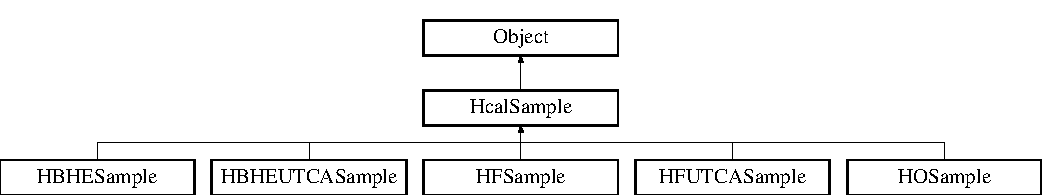
\includegraphics[height=2.625000cm]{class_hcal_sample}
\end{center}
\end{figure}
\subsection*{Public Member Functions}
\begin{DoxyCompactItemize}
\item 
\hyperlink{class_hcal_sample_abda60a97180759affaa1d1b3ab181b6f}{Hcal\+Sample} ()
\item 
\hyperlink{class_hcal_sample_a1b2c66b644d6b16c0bf8efc9f2908db4}{Hcal\+Sample} (\hyperlink{class_collection}{Collection} \&c, unsigned short i, short j)
\item 
virtual float \hyperlink{class_hcal_sample_af837bd894eb8eae865023a526940ee15}{all\+F\+C} ()=0
\item 
virtual float \hyperlink{class_hcal_sample_a603c4e95d1d49db37dd00f34275fb8f3}{energy} ()=0
\item 
virtual float \hyperlink{class_hcal_sample_aefc3dd058b3b178917583ca6abbf4f01}{gain} ()=0
\item 
virtual float \hyperlink{class_hcal_sample_aed932c9f932eabed9f9bc6b1a54c20dd}{fc} ()=0
\item 
virtual float \hyperlink{class_hcal_sample_a9f47a5b867c94c97c3d553e244e7dc87}{nom\+F\+C} ()=0
\item 
virtual float \hyperlink{class_hcal_sample_a471f7ef87944ac870ea884a0cc957744}{ped\+F\+C} ()=0
\item 
virtual float \hyperlink{class_hcal_sample_a6fd32da2d5ea80154251de366f98c49c}{rc\+Gain} ()=0
\item 
virtual int \hyperlink{class_hcal_sample_a3801777ac080ca0e512c226e4cfd5682}{adc} ()=0
\item 
virtual int \hyperlink{class_hcal_sample_a51a82042ba140a68f9659140c48d83bc}{capid} ()=0
\item 
virtual int \hyperlink{class_hcal_sample_a13c0e851a42d3122c7bba32d81e31d19}{dv} ()=0
\item 
virtual int \hyperlink{class_hcal_sample_af1805d239ccbc17a6c307d66522da618}{er} ()=0
\item 
virtual int \hyperlink{class_hcal_sample_a5ae9a4d213b69f5ee382c7a6b31eb446}{fiber} ()=0
\item 
virtual int \hyperlink{class_hcal_sample_acdd36acaedfe4e1a6114e6c56d1ed996}{fiber\+Chan} ()=0
\item 
virtual int \hyperlink{class_hcal_sample_a328a0f8f80a0aae47a92500297635bd6}{raw} ()=0
\item 
double \& \hyperlink{class_hcal_sample_a06504eff6a267228754fead92c9e4955}{Pt} ()
\item 
double \& \hyperlink{class_hcal_sample_abf85f43fdc3f12861443834c97e3d3eb}{Eta} ()
\item 
double \& \hyperlink{class_hcal_sample_a39d0dd1ee5a627691cfefd92a05f7a2e}{Phi} ()
\item 
bool \hyperlink{class_hcal_sample_a46c1dc16f0be38259e07a93f26cccd73}{Pass\+User\+I\+D} (\hyperlink{_i_d_types_8h_a094c367727273b4da2b960ca3b3edc06}{I\+D}, bool)
\end{DoxyCompactItemize}
\subsection*{Protected Attributes}
\begin{DoxyCompactItemize}
\item 
int \hyperlink{class_hcal_sample_a2ad2497d17da524bd197b9ca6802388e}{m\+\_\+timeslice}
\item 
double \hyperlink{class_hcal_sample_a112304ae8464aa39317050f94e517384}{m\+\_\+null\+\_\+value}
\end{DoxyCompactItemize}


\subsection{Constructor \& Destructor Documentation}
\hypertarget{class_hcal_sample_abda60a97180759affaa1d1b3ab181b6f}{}\index{Hcal\+Sample@{Hcal\+Sample}!Hcal\+Sample@{Hcal\+Sample}}
\index{Hcal\+Sample@{Hcal\+Sample}!Hcal\+Sample@{Hcal\+Sample}}
\subsubsection[{Hcal\+Sample()}]{\setlength{\rightskip}{0pt plus 5cm}Hcal\+Sample\+::\+Hcal\+Sample (
\begin{DoxyParamCaption}
{}
\end{DoxyParamCaption}
)}\label{class_hcal_sample_abda60a97180759affaa1d1b3ab181b6f}
\hypertarget{class_hcal_sample_a1b2c66b644d6b16c0bf8efc9f2908db4}{}\index{Hcal\+Sample@{Hcal\+Sample}!Hcal\+Sample@{Hcal\+Sample}}
\index{Hcal\+Sample@{Hcal\+Sample}!Hcal\+Sample@{Hcal\+Sample}}
\subsubsection[{Hcal\+Sample(\+Collection \&c, unsigned short i, short j)}]{\setlength{\rightskip}{0pt plus 5cm}Hcal\+Sample\+::\+Hcal\+Sample (
\begin{DoxyParamCaption}
\item[{{\bf Collection} \&}]{c, }
\item[{unsigned short}]{i, }
\item[{short}]{j}
\end{DoxyParamCaption}
)}\label{class_hcal_sample_a1b2c66b644d6b16c0bf8efc9f2908db4}


\subsection{Member Function Documentation}
\hypertarget{class_hcal_sample_a3801777ac080ca0e512c226e4cfd5682}{}\index{Hcal\+Sample@{Hcal\+Sample}!adc@{adc}}
\index{adc@{adc}!Hcal\+Sample@{Hcal\+Sample}}
\subsubsection[{adc()=0}]{\setlength{\rightskip}{0pt plus 5cm}virtual int Hcal\+Sample\+::adc (
\begin{DoxyParamCaption}
{}
\end{DoxyParamCaption}
)\hspace{0.3cm}{\ttfamily [pure virtual]}}\label{class_hcal_sample_a3801777ac080ca0e512c226e4cfd5682}


Implemented in \hyperlink{class_h_b_h_e_sample_a0519407431ebef16ff6e1df63551b99f}{H\+B\+H\+E\+Sample}, \hyperlink{class_h_b_h_e_u_t_c_a_sample_a9590d80a50ee9679e283bcc1d0896ea1}{H\+B\+H\+E\+U\+T\+C\+A\+Sample}, \hyperlink{class_h_f_sample_a6de90bbb0f186174e2c4c8788a7f7d46}{H\+F\+Sample}, \hyperlink{class_h_f_u_t_c_a_sample_a6923b32caebe543bcc220c0079aaaede}{H\+F\+U\+T\+C\+A\+Sample}, and \hyperlink{class_h_o_sample_adb4388064b1512918b527fa0ded051e1}{H\+O\+Sample}.

\hypertarget{class_hcal_sample_af837bd894eb8eae865023a526940ee15}{}\index{Hcal\+Sample@{Hcal\+Sample}!all\+F\+C@{all\+F\+C}}
\index{all\+F\+C@{all\+F\+C}!Hcal\+Sample@{Hcal\+Sample}}
\subsubsection[{all\+F\+C()=0}]{\setlength{\rightskip}{0pt plus 5cm}virtual float Hcal\+Sample\+::all\+F\+C (
\begin{DoxyParamCaption}
{}
\end{DoxyParamCaption}
)\hspace{0.3cm}{\ttfamily [pure virtual]}}\label{class_hcal_sample_af837bd894eb8eae865023a526940ee15}


Implemented in \hyperlink{class_h_b_h_e_sample_ac674f791c79264801dbedd14c2cd88c7}{H\+B\+H\+E\+Sample}, \hyperlink{class_h_b_h_e_u_t_c_a_sample_adc02ae534bdfa6b4deee50da12fc638d}{H\+B\+H\+E\+U\+T\+C\+A\+Sample}, \hyperlink{class_h_f_sample_a8903a7d7f5dcc3cfc57be371e1a61d11}{H\+F\+Sample}, \hyperlink{class_h_f_u_t_c_a_sample_aca1a7db39701544c65d02b5b643a8752}{H\+F\+U\+T\+C\+A\+Sample}, and \hyperlink{class_h_o_sample_a7517db4397842a88372e74a0e769d270}{H\+O\+Sample}.

\hypertarget{class_hcal_sample_a51a82042ba140a68f9659140c48d83bc}{}\index{Hcal\+Sample@{Hcal\+Sample}!capid@{capid}}
\index{capid@{capid}!Hcal\+Sample@{Hcal\+Sample}}
\subsubsection[{capid()=0}]{\setlength{\rightskip}{0pt plus 5cm}virtual int Hcal\+Sample\+::capid (
\begin{DoxyParamCaption}
{}
\end{DoxyParamCaption}
)\hspace{0.3cm}{\ttfamily [pure virtual]}}\label{class_hcal_sample_a51a82042ba140a68f9659140c48d83bc}


Implemented in \hyperlink{class_h_b_h_e_sample_a8422a9d26a2ee570186192bf8bb32d13}{H\+B\+H\+E\+Sample}, \hyperlink{class_h_b_h_e_u_t_c_a_sample_aa3428923215b84025833f1f558b70993}{H\+B\+H\+E\+U\+T\+C\+A\+Sample}, \hyperlink{class_h_f_sample_a20b55dedbf364a02ee11f63f66adad86}{H\+F\+Sample}, \hyperlink{class_h_f_u_t_c_a_sample_ac7f68c45087e2c9d457515af56c8febc}{H\+F\+U\+T\+C\+A\+Sample}, and \hyperlink{class_h_o_sample_aae92efbb6b23b511c923a84723811dfe}{H\+O\+Sample}.

\hypertarget{class_hcal_sample_a13c0e851a42d3122c7bba32d81e31d19}{}\index{Hcal\+Sample@{Hcal\+Sample}!dv@{dv}}
\index{dv@{dv}!Hcal\+Sample@{Hcal\+Sample}}
\subsubsection[{dv()=0}]{\setlength{\rightskip}{0pt plus 5cm}virtual int Hcal\+Sample\+::dv (
\begin{DoxyParamCaption}
{}
\end{DoxyParamCaption}
)\hspace{0.3cm}{\ttfamily [pure virtual]}}\label{class_hcal_sample_a13c0e851a42d3122c7bba32d81e31d19}


Implemented in \hyperlink{class_h_b_h_e_sample_a3baa7c7a60db7c5e01ed8d5861cb2093}{H\+B\+H\+E\+Sample}, \hyperlink{class_h_b_h_e_u_t_c_a_sample_a804ca3a58ef7f4500639fdd22622e9dd}{H\+B\+H\+E\+U\+T\+C\+A\+Sample}, \hyperlink{class_h_f_sample_a57495b56198eb49caf8f34b1554969f9}{H\+F\+Sample}, \hyperlink{class_h_f_u_t_c_a_sample_a95f366e87ccd669a0fdb69363c71aefb}{H\+F\+U\+T\+C\+A\+Sample}, and \hyperlink{class_h_o_sample_a3fcb610100099d07f030249da9160aaa}{H\+O\+Sample}.

\hypertarget{class_hcal_sample_a603c4e95d1d49db37dd00f34275fb8f3}{}\index{Hcal\+Sample@{Hcal\+Sample}!energy@{energy}}
\index{energy@{energy}!Hcal\+Sample@{Hcal\+Sample}}
\subsubsection[{energy()=0}]{\setlength{\rightskip}{0pt plus 5cm}virtual float Hcal\+Sample\+::energy (
\begin{DoxyParamCaption}
{}
\end{DoxyParamCaption}
)\hspace{0.3cm}{\ttfamily [pure virtual]}}\label{class_hcal_sample_a603c4e95d1d49db37dd00f34275fb8f3}


Implemented in \hyperlink{class_h_b_h_e_sample_aaf6e464f53e1927e8c81c9d45bf5edd7}{H\+B\+H\+E\+Sample}, \hyperlink{class_h_b_h_e_u_t_c_a_sample_a16cce3e525f59c9d92dc08fb9b685852}{H\+B\+H\+E\+U\+T\+C\+A\+Sample}, \hyperlink{class_h_f_sample_ab6021ff226750df9c11bfa8a9ae956eb}{H\+F\+Sample}, \hyperlink{class_h_f_u_t_c_a_sample_abd8d7c0f338668db3d18a2a79493e1ec}{H\+F\+U\+T\+C\+A\+Sample}, and \hyperlink{class_h_o_sample_a94767275b31209a74a9d8169ee88276d}{H\+O\+Sample}.

\hypertarget{class_hcal_sample_af1805d239ccbc17a6c307d66522da618}{}\index{Hcal\+Sample@{Hcal\+Sample}!er@{er}}
\index{er@{er}!Hcal\+Sample@{Hcal\+Sample}}
\subsubsection[{er()=0}]{\setlength{\rightskip}{0pt plus 5cm}virtual int Hcal\+Sample\+::er (
\begin{DoxyParamCaption}
{}
\end{DoxyParamCaption}
)\hspace{0.3cm}{\ttfamily [pure virtual]}}\label{class_hcal_sample_af1805d239ccbc17a6c307d66522da618}


Implemented in \hyperlink{class_h_b_h_e_sample_a54f776ae3bda86074cc5449871588b8c}{H\+B\+H\+E\+Sample}, \hyperlink{class_h_b_h_e_u_t_c_a_sample_a02c629e33022099b919fba9e69b15054}{H\+B\+H\+E\+U\+T\+C\+A\+Sample}, \hyperlink{class_h_f_sample_a38c50f0bec2401db64258670b423acd9}{H\+F\+Sample}, \hyperlink{class_h_f_u_t_c_a_sample_a26ede18ebc816eb8f5de7f1073566f7f}{H\+F\+U\+T\+C\+A\+Sample}, and \hyperlink{class_h_o_sample_ae63dde72730e4ab5a08e0b4b5a0ba19e}{H\+O\+Sample}.

\hypertarget{class_hcal_sample_abf85f43fdc3f12861443834c97e3d3eb}{}\index{Hcal\+Sample@{Hcal\+Sample}!Eta@{Eta}}
\index{Eta@{Eta}!Hcal\+Sample@{Hcal\+Sample}}
\subsubsection[{Eta()}]{\setlength{\rightskip}{0pt plus 5cm}double\& Hcal\+Sample\+::\+Eta (
\begin{DoxyParamCaption}
{}
\end{DoxyParamCaption}
)\hspace{0.3cm}{\ttfamily [inline]}, {\ttfamily [virtual]}}\label{class_hcal_sample_abf85f43fdc3f12861443834c97e3d3eb}


Implements \hyperlink{class_object_a3760d2b4b0723118234370675654d46a}{Object}.

\hypertarget{class_hcal_sample_aed932c9f932eabed9f9bc6b1a54c20dd}{}\index{Hcal\+Sample@{Hcal\+Sample}!fc@{fc}}
\index{fc@{fc}!Hcal\+Sample@{Hcal\+Sample}}
\subsubsection[{fc()=0}]{\setlength{\rightskip}{0pt plus 5cm}virtual float Hcal\+Sample\+::fc (
\begin{DoxyParamCaption}
{}
\end{DoxyParamCaption}
)\hspace{0.3cm}{\ttfamily [pure virtual]}}\label{class_hcal_sample_aed932c9f932eabed9f9bc6b1a54c20dd}


Implemented in \hyperlink{class_h_b_h_e_sample_acb53267f00c5eda17d44e8e08cd97752}{H\+B\+H\+E\+Sample}, \hyperlink{class_h_b_h_e_u_t_c_a_sample_a5792dd730d0c9051db9c4ef9dae69c32}{H\+B\+H\+E\+U\+T\+C\+A\+Sample}, \hyperlink{class_h_f_sample_a02a219abba2029e93e0740d966ba0caf}{H\+F\+Sample}, \hyperlink{class_h_f_u_t_c_a_sample_a41761d51c05dfbdf0c5da9be026dd773}{H\+F\+U\+T\+C\+A\+Sample}, and \hyperlink{class_h_o_sample_aca3d42b2fd9431719f849542ebfdf2a9}{H\+O\+Sample}.

\hypertarget{class_hcal_sample_a5ae9a4d213b69f5ee382c7a6b31eb446}{}\index{Hcal\+Sample@{Hcal\+Sample}!fiber@{fiber}}
\index{fiber@{fiber}!Hcal\+Sample@{Hcal\+Sample}}
\subsubsection[{fiber()=0}]{\setlength{\rightskip}{0pt plus 5cm}virtual int Hcal\+Sample\+::fiber (
\begin{DoxyParamCaption}
{}
\end{DoxyParamCaption}
)\hspace{0.3cm}{\ttfamily [pure virtual]}}\label{class_hcal_sample_a5ae9a4d213b69f5ee382c7a6b31eb446}


Implemented in \hyperlink{class_h_b_h_e_sample_a65cb719fc34ef056908006c63dc1e35f}{H\+B\+H\+E\+Sample}, \hyperlink{class_h_b_h_e_u_t_c_a_sample_a99f62813e4808dfead59ab54846ec54a}{H\+B\+H\+E\+U\+T\+C\+A\+Sample}, \hyperlink{class_h_f_sample_a048dea0ef5de5cf9904fb2397427d6f4}{H\+F\+Sample}, \hyperlink{class_h_f_u_t_c_a_sample_aa9987206c078a46d3a41f5327c3bd83c}{H\+F\+U\+T\+C\+A\+Sample}, and \hyperlink{class_h_o_sample_a59d656a291cb5e7242c27fed2346a3a7}{H\+O\+Sample}.

\hypertarget{class_hcal_sample_acdd36acaedfe4e1a6114e6c56d1ed996}{}\index{Hcal\+Sample@{Hcal\+Sample}!fiber\+Chan@{fiber\+Chan}}
\index{fiber\+Chan@{fiber\+Chan}!Hcal\+Sample@{Hcal\+Sample}}
\subsubsection[{fiber\+Chan()=0}]{\setlength{\rightskip}{0pt plus 5cm}virtual int Hcal\+Sample\+::fiber\+Chan (
\begin{DoxyParamCaption}
{}
\end{DoxyParamCaption}
)\hspace{0.3cm}{\ttfamily [pure virtual]}}\label{class_hcal_sample_acdd36acaedfe4e1a6114e6c56d1ed996}


Implemented in \hyperlink{class_h_b_h_e_sample_a87b6f6251cf487f49f98e914938cd26b}{H\+B\+H\+E\+Sample}, \hyperlink{class_h_b_h_e_u_t_c_a_sample_a5f57f71833cd7650af5361b4cb2a22e2}{H\+B\+H\+E\+U\+T\+C\+A\+Sample}, \hyperlink{class_h_f_sample_a82342cdd81bc6252e8272a4ff1961d08}{H\+F\+Sample}, \hyperlink{class_h_f_u_t_c_a_sample_acab9631919ea67506b229f7ac80a975f}{H\+F\+U\+T\+C\+A\+Sample}, and \hyperlink{class_h_o_sample_a136f3641f4e0cafd6270fe4006acd499}{H\+O\+Sample}.

\hypertarget{class_hcal_sample_aefc3dd058b3b178917583ca6abbf4f01}{}\index{Hcal\+Sample@{Hcal\+Sample}!gain@{gain}}
\index{gain@{gain}!Hcal\+Sample@{Hcal\+Sample}}
\subsubsection[{gain()=0}]{\setlength{\rightskip}{0pt plus 5cm}virtual float Hcal\+Sample\+::gain (
\begin{DoxyParamCaption}
{}
\end{DoxyParamCaption}
)\hspace{0.3cm}{\ttfamily [pure virtual]}}\label{class_hcal_sample_aefc3dd058b3b178917583ca6abbf4f01}


Implemented in \hyperlink{class_h_b_h_e_sample_a213cba0c1dfac7f9c81e4bb89d1a096d}{H\+B\+H\+E\+Sample}, \hyperlink{class_h_b_h_e_u_t_c_a_sample_a5c7b26e64ac924f511411024b87cb669}{H\+B\+H\+E\+U\+T\+C\+A\+Sample}, \hyperlink{class_h_f_sample_a210b2ca2173c8267e3c3ba86bcad3e96}{H\+F\+Sample}, \hyperlink{class_h_f_u_t_c_a_sample_abda1fe3f4fd86f464fa1101469fda074}{H\+F\+U\+T\+C\+A\+Sample}, and \hyperlink{class_h_o_sample_adc4aeb23e36cea824ce18dbdf57ffbc2}{H\+O\+Sample}.

\hypertarget{class_hcal_sample_a9f47a5b867c94c97c3d553e244e7dc87}{}\index{Hcal\+Sample@{Hcal\+Sample}!nom\+F\+C@{nom\+F\+C}}
\index{nom\+F\+C@{nom\+F\+C}!Hcal\+Sample@{Hcal\+Sample}}
\subsubsection[{nom\+F\+C()=0}]{\setlength{\rightskip}{0pt plus 5cm}virtual float Hcal\+Sample\+::nom\+F\+C (
\begin{DoxyParamCaption}
{}
\end{DoxyParamCaption}
)\hspace{0.3cm}{\ttfamily [pure virtual]}}\label{class_hcal_sample_a9f47a5b867c94c97c3d553e244e7dc87}


Implemented in \hyperlink{class_h_b_h_e_sample_a1dffd426b564378da4161b5279da97b6}{H\+B\+H\+E\+Sample}, \hyperlink{class_h_b_h_e_u_t_c_a_sample_ae261168bd8c528c76f8ef7ded47651a6}{H\+B\+H\+E\+U\+T\+C\+A\+Sample}, \hyperlink{class_h_f_sample_a4356ce2fc34149ba580f72609565f9b8}{H\+F\+Sample}, \hyperlink{class_h_f_u_t_c_a_sample_a989c287e356b37be8886e93865d7a16a}{H\+F\+U\+T\+C\+A\+Sample}, and \hyperlink{class_h_o_sample_a403853f4477960ae93988c5629a28c0c}{H\+O\+Sample}.

\hypertarget{class_hcal_sample_a46c1dc16f0be38259e07a93f26cccd73}{}\index{Hcal\+Sample@{Hcal\+Sample}!Pass\+User\+I\+D@{Pass\+User\+I\+D}}
\index{Pass\+User\+I\+D@{Pass\+User\+I\+D}!Hcal\+Sample@{Hcal\+Sample}}
\subsubsection[{Pass\+User\+I\+D(\+I\+D, bool)}]{\setlength{\rightskip}{0pt plus 5cm}bool Hcal\+Sample\+::\+Pass\+User\+I\+D (
\begin{DoxyParamCaption}
\item[{{\bf I\+D}}]{, }
\item[{bool}]{}
\end{DoxyParamCaption}
)\hspace{0.3cm}{\ttfamily [inline]}, {\ttfamily [virtual]}}\label{class_hcal_sample_a46c1dc16f0be38259e07a93f26cccd73}


Implements \hyperlink{class_object_ae28bc9879447dad23f10ebd1971e81f5}{Object}.

\hypertarget{class_hcal_sample_a471f7ef87944ac870ea884a0cc957744}{}\index{Hcal\+Sample@{Hcal\+Sample}!ped\+F\+C@{ped\+F\+C}}
\index{ped\+F\+C@{ped\+F\+C}!Hcal\+Sample@{Hcal\+Sample}}
\subsubsection[{ped\+F\+C()=0}]{\setlength{\rightskip}{0pt plus 5cm}virtual float Hcal\+Sample\+::ped\+F\+C (
\begin{DoxyParamCaption}
{}
\end{DoxyParamCaption}
)\hspace{0.3cm}{\ttfamily [pure virtual]}}\label{class_hcal_sample_a471f7ef87944ac870ea884a0cc957744}


Implemented in \hyperlink{class_h_b_h_e_sample_afeaa57de45b3ad755e91ba154adf9c78}{H\+B\+H\+E\+Sample}, \hyperlink{class_h_b_h_e_u_t_c_a_sample_a0dc80ef00077e32025a6db5fc8d3fe3b}{H\+B\+H\+E\+U\+T\+C\+A\+Sample}, \hyperlink{class_h_f_sample_ad99d42390ac0646749acd988680d750d}{H\+F\+Sample}, \hyperlink{class_h_f_u_t_c_a_sample_a2bf5628c13f9908c0dc6606f2b8580c5}{H\+F\+U\+T\+C\+A\+Sample}, and \hyperlink{class_h_o_sample_afccd544265c85885bce27d960aa81741}{H\+O\+Sample}.

\hypertarget{class_hcal_sample_a39d0dd1ee5a627691cfefd92a05f7a2e}{}\index{Hcal\+Sample@{Hcal\+Sample}!Phi@{Phi}}
\index{Phi@{Phi}!Hcal\+Sample@{Hcal\+Sample}}
\subsubsection[{Phi()}]{\setlength{\rightskip}{0pt plus 5cm}double\& Hcal\+Sample\+::\+Phi (
\begin{DoxyParamCaption}
{}
\end{DoxyParamCaption}
)\hspace{0.3cm}{\ttfamily [inline]}, {\ttfamily [virtual]}}\label{class_hcal_sample_a39d0dd1ee5a627691cfefd92a05f7a2e}


Implements \hyperlink{class_object_ab8fa3bfbd16c2b6c420ec113fbc2a0e4}{Object}.

\hypertarget{class_hcal_sample_a06504eff6a267228754fead92c9e4955}{}\index{Hcal\+Sample@{Hcal\+Sample}!Pt@{Pt}}
\index{Pt@{Pt}!Hcal\+Sample@{Hcal\+Sample}}
\subsubsection[{Pt()}]{\setlength{\rightskip}{0pt plus 5cm}double\& Hcal\+Sample\+::\+Pt (
\begin{DoxyParamCaption}
{}
\end{DoxyParamCaption}
)\hspace{0.3cm}{\ttfamily [inline]}, {\ttfamily [virtual]}}\label{class_hcal_sample_a06504eff6a267228754fead92c9e4955}


Implements \hyperlink{class_object_ac280f2330a4bd359404841431bd46f2e}{Object}.

\hypertarget{class_hcal_sample_a328a0f8f80a0aae47a92500297635bd6}{}\index{Hcal\+Sample@{Hcal\+Sample}!raw@{raw}}
\index{raw@{raw}!Hcal\+Sample@{Hcal\+Sample}}
\subsubsection[{raw()=0}]{\setlength{\rightskip}{0pt plus 5cm}virtual int Hcal\+Sample\+::raw (
\begin{DoxyParamCaption}
{}
\end{DoxyParamCaption}
)\hspace{0.3cm}{\ttfamily [pure virtual]}}\label{class_hcal_sample_a328a0f8f80a0aae47a92500297635bd6}


Implemented in \hyperlink{class_h_b_h_e_sample_ac72e5201bf29d9460694bf65311ba9b7}{H\+B\+H\+E\+Sample}, \hyperlink{class_h_b_h_e_u_t_c_a_sample_aa6673645bd8dec6413065dd5d426b0b8}{H\+B\+H\+E\+U\+T\+C\+A\+Sample}, \hyperlink{class_h_f_sample_a2709fd941ccbbb029bbbbdd07ceb83f4}{H\+F\+Sample}, \hyperlink{class_h_f_u_t_c_a_sample_a8aba41a05a990528d3bd3dada9e2fc91}{H\+F\+U\+T\+C\+A\+Sample}, and \hyperlink{class_h_o_sample_ad4e252cf8313d9072f7162df3ac4c5af}{H\+O\+Sample}.

\hypertarget{class_hcal_sample_a6fd32da2d5ea80154251de366f98c49c}{}\index{Hcal\+Sample@{Hcal\+Sample}!rc\+Gain@{rc\+Gain}}
\index{rc\+Gain@{rc\+Gain}!Hcal\+Sample@{Hcal\+Sample}}
\subsubsection[{rc\+Gain()=0}]{\setlength{\rightskip}{0pt plus 5cm}virtual float Hcal\+Sample\+::rc\+Gain (
\begin{DoxyParamCaption}
{}
\end{DoxyParamCaption}
)\hspace{0.3cm}{\ttfamily [pure virtual]}}\label{class_hcal_sample_a6fd32da2d5ea80154251de366f98c49c}


Implemented in \hyperlink{class_h_b_h_e_sample_ab03c24466f72bce782a3fcf62df15e5f}{H\+B\+H\+E\+Sample}, \hyperlink{class_h_b_h_e_u_t_c_a_sample_a7817d78373bf3a36594ebb581a08fb4c}{H\+B\+H\+E\+U\+T\+C\+A\+Sample}, \hyperlink{class_h_f_sample_aebbfa0a6e0596461bc8585551e12fd38}{H\+F\+Sample}, \hyperlink{class_h_f_u_t_c_a_sample_a0052d9a14ddb41b55e1e5e1983fc9684}{H\+F\+U\+T\+C\+A\+Sample}, and \hyperlink{class_h_o_sample_aed754b102ffe962139bb216df35a308f}{H\+O\+Sample}.



\subsection{Member Data Documentation}
\hypertarget{class_hcal_sample_a112304ae8464aa39317050f94e517384}{}\index{Hcal\+Sample@{Hcal\+Sample}!m\+\_\+null\+\_\+value@{m\+\_\+null\+\_\+value}}
\index{m\+\_\+null\+\_\+value@{m\+\_\+null\+\_\+value}!Hcal\+Sample@{Hcal\+Sample}}
\subsubsection[{m\+\_\+null\+\_\+value}]{\setlength{\rightskip}{0pt plus 5cm}double Hcal\+Sample\+::m\+\_\+null\+\_\+value\hspace{0.3cm}{\ttfamily [protected]}}\label{class_hcal_sample_a112304ae8464aa39317050f94e517384}
\hypertarget{class_hcal_sample_a2ad2497d17da524bd197b9ca6802388e}{}\index{Hcal\+Sample@{Hcal\+Sample}!m\+\_\+timeslice@{m\+\_\+timeslice}}
\index{m\+\_\+timeslice@{m\+\_\+timeslice}!Hcal\+Sample@{Hcal\+Sample}}
\subsubsection[{m\+\_\+timeslice}]{\setlength{\rightskip}{0pt plus 5cm}int Hcal\+Sample\+::m\+\_\+timeslice\hspace{0.3cm}{\ttfamily [protected]}}\label{class_hcal_sample_a2ad2497d17da524bd197b9ca6802388e}


The documentation for this class was generated from the following files\+:\begin{DoxyCompactItemize}
\item 
interface/\hyperlink{_hcal_sample_8h}{Hcal\+Sample.\+h}\item 
src/\hyperlink{_hcal_sample_8cc}{Hcal\+Sample.\+cc}\end{DoxyCompactItemize}

\hypertarget{class_hcal_tuple_tree}{}\section{Hcal\+Tuple\+Tree Class Reference}
\label{class_hcal_tuple_tree}\index{Hcal\+Tuple\+Tree@{Hcal\+Tuple\+Tree}}


{\ttfamily \#include $<$Hcal\+Tuple\+Tree.\+h$>$}

Inheritance diagram for Hcal\+Tuple\+Tree\+:\begin{figure}[H]
\begin{center}
\leavevmode
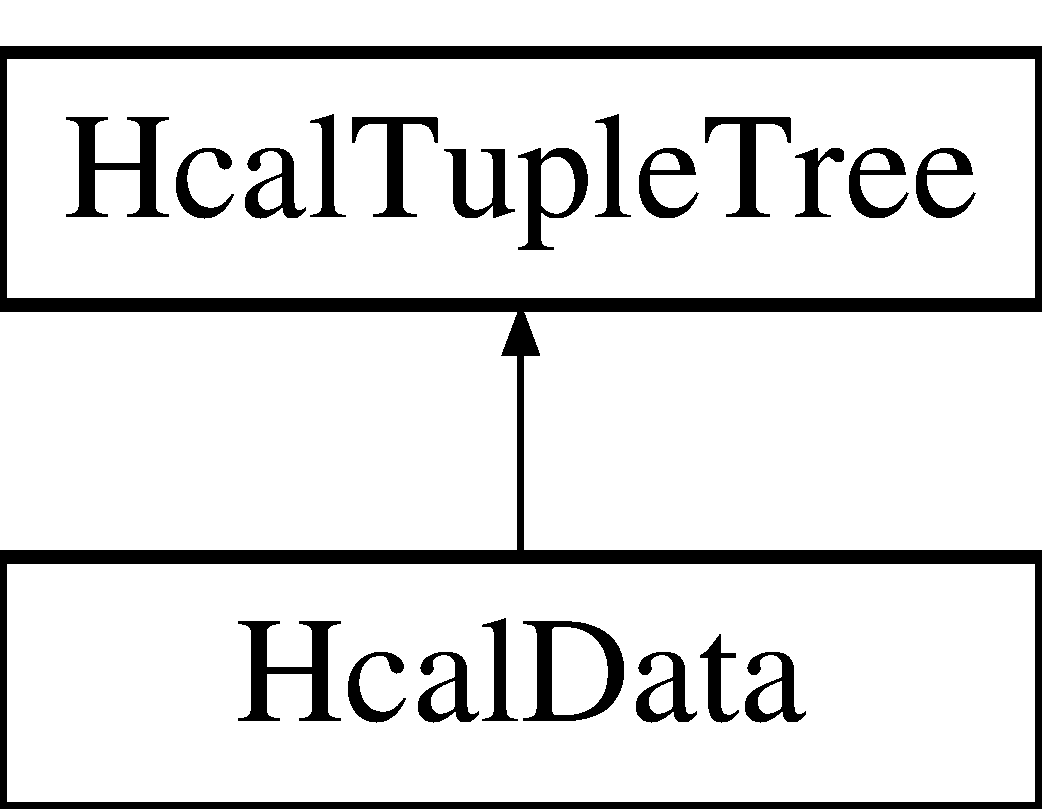
\includegraphics[height=2.000000cm]{class_hcal_tuple_tree}
\end{center}
\end{figure}
\subsection*{Public Member Functions}
\begin{DoxyCompactItemize}
\item 
\hyperlink{class_hcal_tuple_tree_a93a2b9686fd32bc3145c0653c2255203}{Hcal\+Tuple\+Tree} (T\+Tree $\ast$tree=0)
\item 
virtual \hyperlink{class_hcal_tuple_tree_a2bba2f967fd63217177ec8275f4378d1}{$\sim$\+Hcal\+Tuple\+Tree} ()
\item 
virtual Int\+\_\+t \hyperlink{class_hcal_tuple_tree_a3c6f115f9de0929d577fd3fee90ab347}{Cut} (Long64\+\_\+t entry)
\item 
virtual Int\+\_\+t \hyperlink{class_hcal_tuple_tree_a61ac2553042cf88a12bd462a7814c18d}{Get\+Entry} (Long64\+\_\+t entry)
\item 
virtual Long64\+\_\+t \hyperlink{class_hcal_tuple_tree_ae02bb52e1602961c2d50eb112a539ab2}{Load\+Tree} (Long64\+\_\+t entry)
\item 
virtual void \hyperlink{class_hcal_tuple_tree_ad624a0b1c545a1aade5b6c1af6f680f9}{Init} (T\+Tree $\ast$tree)
\item 
virtual void \hyperlink{class_hcal_tuple_tree_a2786184220161c1733fe48f6b729ad03}{Loop} ()
\item 
virtual Bool\+\_\+t \hyperlink{class_hcal_tuple_tree_a96cea8c5f1ff0a479fa1f5f46267fd1d}{Notify} ()
\item 
virtual void \hyperlink{class_hcal_tuple_tree_ab48299f2334cd356df44d4d695e4f6c6}{Show} (Long64\+\_\+t entry=-\/1)
\end{DoxyCompactItemize}
\subsection*{Public Attributes}
\begin{DoxyCompactItemize}
\item 
T\+Tree $\ast$ \hyperlink{class_hcal_tuple_tree_ab2d0b951f1d870277db06338998d359c}{f\+Chain}
\item 
Int\+\_\+t \hyperlink{class_hcal_tuple_tree_a08b8ee5bd18d61d595dabae8738f94f0}{f\+Current}
\begin{DoxyCompactList}\small\item\em pointer to the analyzed T\+Tree or T\+Chain \end{DoxyCompactList}\item 
vector$<$ float $>$ $\ast$ \hyperlink{class_hcal_tuple_tree_abf3ece84d6c5e826fe0afe18259efdf6}{H\+B\+H\+E\+Digi\+Eta}
\begin{DoxyCompactList}\small\item\em current Tree number in a T\+Chain \end{DoxyCompactList}\item 
vector$<$ float $>$ $\ast$ \hyperlink{class_hcal_tuple_tree_a4465ac5c76bde5c83e2c0440e94377e6}{H\+B\+H\+E\+Digi\+Phi}
\item 
vector$<$ float $>$ $\ast$ \hyperlink{class_hcal_tuple_tree_a71d33dc8870ce67415396153c1c0b8fc}{H\+B\+H\+E\+Digi\+Rec\+Energy}
\item 
vector$<$ float $>$ $\ast$ \hyperlink{class_hcal_tuple_tree_a932a5241aeb73633d88a523951bd04b7}{H\+B\+H\+E\+Digi\+Rec\+Time}
\item 
vector$<$ float $>$ $\ast$ \hyperlink{class_hcal_tuple_tree_a4ee87b23a35d035afec70d98d6c319aa}{H\+F\+Digi\+Eta}
\item 
vector$<$ float $>$ $\ast$ \hyperlink{class_hcal_tuple_tree_a778805ed9ac0fb9bd7c0ada3adfb05ef}{H\+F\+Digi\+Phi}
\item 
vector$<$ float $>$ $\ast$ \hyperlink{class_hcal_tuple_tree_a3e26e7151e6cbba42bee136f6e46e07e}{H\+F\+Digi\+Rec\+Energy}
\item 
vector$<$ float $>$ $\ast$ \hyperlink{class_hcal_tuple_tree_af95d1984176d950add73dc9d411cda04}{H\+F\+Digi\+Rec\+Time}
\item 
vector$<$ float $>$ $\ast$ \hyperlink{class_hcal_tuple_tree_af4c462a15fc5e42100dc88e4eaa16f1e}{H\+O\+Digi\+Eta}
\item 
vector$<$ float $>$ $\ast$ \hyperlink{class_hcal_tuple_tree_a31ee04dc7198ca962dfaf857a6e19339}{H\+O\+Digi\+Phi}
\item 
vector$<$ float $>$ $\ast$ \hyperlink{class_hcal_tuple_tree_a74256e07cba2a77b6d96c50e5dbcab2f}{H\+O\+Digi\+Rec\+Energy}
\item 
vector$<$ float $>$ $\ast$ \hyperlink{class_hcal_tuple_tree_a518d0a94b9cc0ca05a72210dd907a932}{H\+O\+Digi\+Rec\+Time}
\item 
vector$<$ vector$<$ float $>$ $>$ $\ast$ \hyperlink{class_hcal_tuple_tree_a5dc5cdeb59f28eaa2308daa56474c892}{H\+B\+H\+E\+Digi\+All\+F\+C}
\item 
vector$<$ vector$<$ float $>$ $>$ $\ast$ \hyperlink{class_hcal_tuple_tree_ae64aeab5ce5b05e5b0e8c140bba901b1}{H\+B\+H\+E\+Digi\+Energy}
\item 
vector$<$ vector$<$ float $>$ $>$ $\ast$ \hyperlink{class_hcal_tuple_tree_a9146017ce5694aaa1c4616e06218c39c}{H\+B\+H\+E\+Digi\+F\+C}
\item 
vector$<$ vector$<$ float $>$ $>$ $\ast$ \hyperlink{class_hcal_tuple_tree_a2bb6e71cd46bf0e2fdbccce0d141d506}{H\+B\+H\+E\+Digi\+Gain}
\item 
vector$<$ vector$<$ float $>$ $>$ $\ast$ \hyperlink{class_hcal_tuple_tree_aa829f8de833074383a9758072440a572}{H\+B\+H\+E\+Digi\+Nom\+F\+C}
\item 
vector$<$ vector$<$ float $>$ $>$ $\ast$ \hyperlink{class_hcal_tuple_tree_a75ddbcd15a6c3c15370257f4e18f93dc}{H\+B\+H\+E\+Digi\+Ped\+F\+C}
\item 
vector$<$ vector$<$ float $>$ $>$ $\ast$ \hyperlink{class_hcal_tuple_tree_acbd3f4798c9bd4c991a537d4658eb96e}{H\+B\+H\+E\+Digi\+R\+C\+Gain}
\item 
vector$<$ vector$<$ float $>$ $>$ $\ast$ \hyperlink{class_hcal_tuple_tree_ae9cf3812ae649b0941182c185eb6a721}{H\+F\+Digi\+All\+F\+C}
\item 
vector$<$ vector$<$ float $>$ $>$ $\ast$ \hyperlink{class_hcal_tuple_tree_af4208c69d37152cef6fff1c1dd026155}{H\+F\+Digi\+Energy}
\item 
vector$<$ vector$<$ float $>$ $>$ $\ast$ \hyperlink{class_hcal_tuple_tree_ac47c0113b05b20cdee0a28017cd08724}{H\+F\+Digi\+F\+C}
\item 
vector$<$ vector$<$ float $>$ $>$ $\ast$ \hyperlink{class_hcal_tuple_tree_abc594e1718c4ca609859b9c5da187ce9}{H\+F\+Digi\+Gain}
\item 
vector$<$ vector$<$ float $>$ $>$ $\ast$ \hyperlink{class_hcal_tuple_tree_a237a14d107a2090e46f21ffe7500123d}{H\+F\+Digi\+Nom\+F\+C}
\item 
vector$<$ vector$<$ float $>$ $>$ $\ast$ \hyperlink{class_hcal_tuple_tree_a66aa7dc7b2ca36a103449a29aa6af319}{H\+F\+Digi\+Ped\+F\+C}
\item 
vector$<$ vector$<$ float $>$ $>$ $\ast$ \hyperlink{class_hcal_tuple_tree_a9cc44ef6fd299d20874e0b07eb68b94c}{H\+F\+Digi\+R\+C\+Gain}
\item 
vector$<$ vector$<$ float $>$ $>$ $\ast$ \hyperlink{class_hcal_tuple_tree_afe37a056626eef4c965a339b420171a9}{H\+O\+Digi\+All\+F\+C}
\item 
vector$<$ vector$<$ float $>$ $>$ $\ast$ \hyperlink{class_hcal_tuple_tree_a379a809505a4af9fbdd8ed073cdadebf}{H\+O\+Digi\+Energy}
\item 
vector$<$ vector$<$ float $>$ $>$ $\ast$ \hyperlink{class_hcal_tuple_tree_a285842d23b6b8d21ebed868753ee1e68}{H\+O\+Digi\+F\+C}
\item 
vector$<$ vector$<$ float $>$ $>$ $\ast$ \hyperlink{class_hcal_tuple_tree_ab3d383dc83018d2bc4e468a40af05787}{H\+O\+Digi\+Gain}
\item 
vector$<$ vector$<$ float $>$ $>$ $\ast$ \hyperlink{class_hcal_tuple_tree_a56ee5bb65a6e34d5b0934fad381f2015}{H\+O\+Digi\+Nom\+F\+C}
\item 
vector$<$ vector$<$ float $>$ $>$ $\ast$ \hyperlink{class_hcal_tuple_tree_af4ae835aebd4b9754cde9868afed4d7d}{H\+O\+Digi\+Ped\+F\+C}
\item 
vector$<$ vector$<$ float $>$ $>$ $\ast$ \hyperlink{class_hcal_tuple_tree_a760900f2eccc37b9c8efc78b6af457fa}{H\+O\+Digi\+R\+C\+Gain}
\item 
vector$<$ int $>$ $\ast$ \hyperlink{class_hcal_tuple_tree_ae5ed39ea705aff8363edefc34423426e}{H\+B\+H\+E\+Digi\+Depth}
\item 
vector$<$ int $>$ $\ast$ \hyperlink{class_hcal_tuple_tree_a030e840a1ceb41ce84181c68926aa948}{H\+B\+H\+E\+Digi\+Electronics\+I\+D}
\item 
vector$<$ int $>$ $\ast$ \hyperlink{class_hcal_tuple_tree_aaf4a8badc474e66b2f2918cfd80b5a2a}{H\+B\+H\+E\+Digi\+Fiber\+Idle\+Offset}
\item 
vector$<$ int $>$ $\ast$ \hyperlink{class_hcal_tuple_tree_ac80f55cd8338af07ad6e76357e2bdc02}{H\+B\+H\+E\+Digi\+I\+Eta}
\item 
vector$<$ int $>$ $\ast$ \hyperlink{class_hcal_tuple_tree_af201c74f0517d348fcbe767c156139f2}{H\+B\+H\+E\+Digi\+I\+Phi}
\item 
vector$<$ int $>$ $\ast$ \hyperlink{class_hcal_tuple_tree_aa12edf8c843903084ea22da932cea02b}{H\+B\+H\+E\+Digi\+Presamples}
\item 
vector$<$ int $>$ $\ast$ \hyperlink{class_hcal_tuple_tree_a79e823d5bf62909c8bebc784f6a8ceb9}{H\+B\+H\+E\+Digi\+Raw\+I\+D}
\item 
vector$<$ int $>$ $\ast$ \hyperlink{class_hcal_tuple_tree_a285d80e2b161b7ee52a52e1439db3373}{H\+B\+H\+E\+Digi\+Size}
\item 
vector$<$ int $>$ $\ast$ \hyperlink{class_hcal_tuple_tree_aba0b417a85be88cc0f21e3d2cc19d80d}{H\+B\+H\+E\+Digi\+Subdet}
\item 
vector$<$ int $>$ $\ast$ \hyperlink{class_hcal_tuple_tree_a0e59299846d8138c04f69fe451511dfa}{H\+F\+Digi\+Depth}
\item 
vector$<$ int $>$ $\ast$ \hyperlink{class_hcal_tuple_tree_a9882d2d652d197b5ccdc03234ca08ca3}{H\+F\+Digi\+Electronics\+I\+D}
\item 
vector$<$ int $>$ $\ast$ \hyperlink{class_hcal_tuple_tree_a06e52ec27931ef2fc92bcc0efc8901ba}{H\+F\+Digi\+Fiber\+Idle\+Offset}
\item 
vector$<$ int $>$ $\ast$ \hyperlink{class_hcal_tuple_tree_add1b36acb835d09d747c682fb65ce7c9}{H\+F\+Digi\+I\+Eta}
\item 
vector$<$ int $>$ $\ast$ \hyperlink{class_hcal_tuple_tree_aaba8842e7e41699165e52a3345e36221}{H\+F\+Digi\+I\+Phi}
\item 
vector$<$ int $>$ $\ast$ \hyperlink{class_hcal_tuple_tree_ad7090a8222127b46bd6c6b4cafc79d43}{H\+F\+Digi\+Presamples}
\item 
vector$<$ int $>$ $\ast$ \hyperlink{class_hcal_tuple_tree_a55519617ad78d9e9ec81e88aaa2f7e60}{H\+F\+Digi\+Raw\+I\+D}
\item 
vector$<$ int $>$ $\ast$ \hyperlink{class_hcal_tuple_tree_a49bb2b44d538e77e9d13793881c53d97}{H\+F\+Digi\+Size}
\item 
vector$<$ int $>$ $\ast$ \hyperlink{class_hcal_tuple_tree_a7e6e32f123dcbd48805db8f63c17698e}{H\+F\+Digi\+Subdet}
\item 
vector$<$ int $>$ $\ast$ \hyperlink{class_hcal_tuple_tree_a0de64b4e4a03a43dd7bd54afe6b91121}{H\+O\+Digi\+Depth}
\item 
vector$<$ int $>$ $\ast$ \hyperlink{class_hcal_tuple_tree_af1e174814a68ab2f6d4d38208388b769}{H\+O\+Digi\+Electronics\+I\+D}
\item 
vector$<$ int $>$ $\ast$ \hyperlink{class_hcal_tuple_tree_aaff952a6b231321e8ff459a7be299b89}{H\+O\+Digi\+Fiber\+Idle\+Offset}
\item 
vector$<$ int $>$ $\ast$ \hyperlink{class_hcal_tuple_tree_a5f25a69ba6f14ae239054b745cc2f19c}{H\+O\+Digi\+I\+Eta}
\item 
vector$<$ int $>$ $\ast$ \hyperlink{class_hcal_tuple_tree_a4c609f165405dd9d65e93d84b7b2b08d}{H\+O\+Digi\+I\+Phi}
\item 
vector$<$ int $>$ $\ast$ \hyperlink{class_hcal_tuple_tree_a419defccb7894e4a204632feef490ccf}{H\+O\+Digi\+Presamples}
\item 
vector$<$ int $>$ $\ast$ \hyperlink{class_hcal_tuple_tree_aa5b1adb6d1e454dbaa1c2ea8c6d1ce17}{H\+O\+Digi\+Raw\+I\+D}
\item 
vector$<$ int $>$ $\ast$ \hyperlink{class_hcal_tuple_tree_a474c798a52945bf3edef9637b3577e75}{H\+O\+Digi\+Size}
\item 
vector$<$ int $>$ $\ast$ \hyperlink{class_hcal_tuple_tree_a19e6167120f3b6e5d9a93340ed80d334}{H\+O\+Digi\+Subdet}
\item 
vector$<$ int $>$ $\ast$ \hyperlink{class_hcal_tuple_tree_aff8eb56b17cec378fb0996f850bacec1}{Hcal\+Trigger\+Primitive\+Compressed\+Et\+S\+O\+I}
\item 
vector$<$ int $>$ $\ast$ \hyperlink{class_hcal_tuple_tree_a39066327f0677ba5edc25eb97d3865aa}{Hcal\+Trigger\+Primitive\+Fine\+Grain\+S\+O\+I}
\item 
vector$<$ int $>$ $\ast$ \hyperlink{class_hcal_tuple_tree_a702f080483a7152f714355afded4f4f0}{Hcal\+Trigger\+Primitive\+I\+Eta}
\item 
vector$<$ int $>$ $\ast$ \hyperlink{class_hcal_tuple_tree_a2a2a59eb3b63204e75540d5d7c08a3a5}{Hcal\+Trigger\+Primitive\+I\+Phi}
\item 
vector$<$ int $>$ $\ast$ \hyperlink{class_hcal_tuple_tree_aeaf7e05adf680e56bb139054b889ae08}{Hcal\+Trigger\+Primitive\+Presamples}
\item 
vector$<$ int $>$ $\ast$ \hyperlink{class_hcal_tuple_tree_a340bb0e90c7f033c6013c9bfbeb1a6ed}{Hcal\+Trigger\+Primitive\+Size}
\item 
vector$<$ int $>$ $\ast$ \hyperlink{class_hcal_tuple_tree_a82028d16026e71637ce6c8a37fe19fa2}{Hcal\+Unpacker\+Bad\+Digi\+Depth}
\item 
vector$<$ int $>$ $\ast$ \hyperlink{class_hcal_tuple_tree_a48eec514f2d009bfb583c129ed741c34}{Hcal\+Unpacker\+Bad\+Digi\+I\+Eta}
\item 
vector$<$ int $>$ $\ast$ \hyperlink{class_hcal_tuple_tree_a554c455a205854a1dca3e67222da4003}{Hcal\+Unpacker\+Bad\+Digi\+I\+Phi}
\item 
vector$<$ int $>$ $\ast$ \hyperlink{class_hcal_tuple_tree_a7ae78222f2c842d8047c8e4d43bf2db5}{Hcal\+Unpacker\+Bad\+Digi\+Subdet}
\item 
vector$<$ vector$<$ int $>$ $>$ $\ast$ \hyperlink{class_hcal_tuple_tree_aabfac31abb8a835c19bc571bdd28632d}{H\+B\+H\+E\+Digi\+A\+D\+C}
\item 
vector$<$ vector$<$ int $>$ $>$ $\ast$ \hyperlink{class_hcal_tuple_tree_a300d8be67219f5369ac7ce004f95b554}{H\+B\+H\+E\+Digi\+Cap\+I\+D}
\item 
vector$<$ vector$<$ int $>$ $>$ $\ast$ \hyperlink{class_hcal_tuple_tree_a170d23abeaeed048957ada3b4a15f570}{H\+B\+H\+E\+Digi\+D\+V}
\item 
vector$<$ vector$<$ int $>$ $>$ $\ast$ \hyperlink{class_hcal_tuple_tree_a1d61f55b869a51c062b92a71be950b6f}{H\+B\+H\+E\+Digi\+E\+R}
\item 
vector$<$ vector$<$ int $>$ $>$ $\ast$ \hyperlink{class_hcal_tuple_tree_ae14f61c3fa4bc10c7ca6bd3da8d35efb}{H\+B\+H\+E\+Digi\+Fiber}
\item 
vector$<$ vector$<$ int $>$ $>$ $\ast$ \hyperlink{class_hcal_tuple_tree_a227e7a0df2915b2349bbfb0b5dc7d9c2}{H\+B\+H\+E\+Digi\+Fiber\+Chan}
\item 
vector$<$ vector$<$ int $>$ $>$ $\ast$ \hyperlink{class_hcal_tuple_tree_a011228f536f5778b8f97fce17ddbd714}{H\+B\+H\+E\+Digi\+L\+A\+D\+C}
\item 
vector$<$ vector$<$ int $>$ $>$ $\ast$ \hyperlink{class_hcal_tuple_tree_a7bffd95bc16723e633cfe233e57f21b6}{H\+B\+H\+E\+Digi\+Raw}
\item 
vector$<$ vector$<$ int $>$ $>$ $\ast$ \hyperlink{class_hcal_tuple_tree_a6b10444e0b3e05ebcd322870130dd20e}{H\+F\+Digi\+A\+D\+C}
\item 
vector$<$ vector$<$ int $>$ $>$ $\ast$ \hyperlink{class_hcal_tuple_tree_a6257529e73c5059596f204b05bc8d894}{H\+F\+Digi\+Cap\+I\+D}
\item 
vector$<$ vector$<$ int $>$ $>$ $\ast$ \hyperlink{class_hcal_tuple_tree_adc64a7cf0e29af0c19a864d1ee5541c7}{H\+F\+Digi\+D\+V}
\item 
vector$<$ vector$<$ int $>$ $>$ $\ast$ \hyperlink{class_hcal_tuple_tree_a9a2b7882484368d1d4976f6388d306c7}{H\+F\+Digi\+E\+R}
\item 
vector$<$ vector$<$ int $>$ $>$ $\ast$ \hyperlink{class_hcal_tuple_tree_afa91f65c9740c7625235ef9da5adefc3}{H\+F\+Digi\+Fiber}
\item 
vector$<$ vector$<$ int $>$ $>$ $\ast$ \hyperlink{class_hcal_tuple_tree_a739afd6b2bb92d5fd58d345333531cc9}{H\+F\+Digi\+Fiber\+Chan}
\item 
vector$<$ vector$<$ int $>$ $>$ $\ast$ \hyperlink{class_hcal_tuple_tree_aba96a4641a9750ed5bcc626abbe44c3c}{H\+F\+Digi\+L\+A\+D\+C}
\item 
vector$<$ vector$<$ int $>$ $>$ $\ast$ \hyperlink{class_hcal_tuple_tree_ae3043c51037d009294ec7567b8c9ce01}{H\+F\+Digi\+Raw}
\item 
vector$<$ vector$<$ int $>$ $>$ $\ast$ \hyperlink{class_hcal_tuple_tree_a66f1270b14c4fcf3c3c2152414aa867d}{H\+O\+Digi\+A\+D\+C}
\item 
vector$<$ vector$<$ int $>$ $>$ $\ast$ \hyperlink{class_hcal_tuple_tree_a81df879ffcc93b380edb13aaea8eb689}{H\+O\+Digi\+Cap\+I\+D}
\item 
vector$<$ vector$<$ int $>$ $>$ $\ast$ \hyperlink{class_hcal_tuple_tree_a12d79c1f523b7762cba3fb3e7f9a6290}{H\+O\+Digi\+D\+V}
\item 
vector$<$ vector$<$ int $>$ $>$ $\ast$ \hyperlink{class_hcal_tuple_tree_a541ae5ada795a82a8309b0d3e06a53a3}{H\+O\+Digi\+E\+R}
\item 
vector$<$ vector$<$ int $>$ $>$ $\ast$ \hyperlink{class_hcal_tuple_tree_af0fe6322bab84267ca6092eef461829f}{H\+O\+Digi\+Fiber}
\item 
vector$<$ vector$<$ int $>$ $>$ $\ast$ \hyperlink{class_hcal_tuple_tree_a558b32faee67ce93024ef6b65d39eea8}{H\+O\+Digi\+Fiber\+Chan}
\item 
vector$<$ vector$<$ int $>$ $>$ $\ast$ \hyperlink{class_hcal_tuple_tree_af5bd84878d749154d56e72a85ea99291}{H\+O\+Digi\+L\+A\+D\+C}
\item 
vector$<$ vector$<$ int $>$ $>$ $\ast$ \hyperlink{class_hcal_tuple_tree_ad1871cbc92384941dfc7824c9d3066ea}{H\+O\+Digi\+Raw}
\item 
vector$<$ vector$<$ int $>$ $>$ $\ast$ \hyperlink{class_hcal_tuple_tree_a34ce7962d072f721b08f74274f1559e4}{Hcal\+Trigger\+Primitive\+Compressed\+Et}
\item 
vector$<$ vector$<$ int $>$ $>$ $\ast$ \hyperlink{class_hcal_tuple_tree_ab3e76e89779572ff1a02dd94167df44c}{Hcal\+Trigger\+Primitive\+Fine\+Grain}
\item 
vector$<$ vector$<$ int $>$ $>$ $\ast$ \hyperlink{class_hcal_tuple_tree_af6d68e4006a3145f25130b4f5a3fb600}{Hcal\+Trigger\+Primitive\+H\+B\+H\+E\+Digi\+Index}
\item 
vector$<$ vector$<$ int $>$ $>$ $\ast$ \hyperlink{class_hcal_tuple_tree_ad552a76a8e3b13e2302f8f8c651170b1}{Hcal\+Trigger\+Primitive\+H\+F\+Digi\+Index}
\item 
U\+Int\+\_\+t \hyperlink{class_hcal_tuple_tree_ac8b12f3fd8e1a7f7c17f96de2b7df6d0}{bx}
\item 
U\+Int\+\_\+t \hyperlink{class_hcal_tuple_tree_acf307d3c7425105ab941eaf2b06e5941}{event}
\item 
U\+Int\+\_\+t \hyperlink{class_hcal_tuple_tree_a6a440ac41ccfdf350de9344c160cd2d4}{ls}
\item 
U\+Int\+\_\+t \hyperlink{class_hcal_tuple_tree_a387c336e6d042e9b98d4a7552b42daf0}{run}
\item 
U\+Int\+\_\+t \hyperlink{class_hcal_tuple_tree_aa5836af17158d1bfe24fb78838c8c641}{Hcal\+Unpacker\+Any\+Valid}
\item 
U\+Int\+\_\+t \hyperlink{class_hcal_tuple_tree_a7c773a60c5bbb4114478451b065c4e07}{Hcal\+Unpacker\+B\+S\+Y\+Spigots}
\item 
U\+Int\+\_\+t \hyperlink{class_hcal_tuple_tree_a9dba097a78cfc58eec9ab8e149f20155}{Hcal\+Unpacker\+Bad\+Quality\+Digis}
\item 
U\+Int\+\_\+t \hyperlink{class_hcal_tuple_tree_a32c6d9d87a0fc537de1d48c8cb37423a}{Hcal\+Unpacker\+Empty\+Spigots}
\item 
U\+Int\+\_\+t \hyperlink{class_hcal_tuple_tree_ac97729e4a501486a76c030ad3477fd0d}{Hcal\+Unpacker\+Error\+Free}
\item 
U\+Int\+\_\+t \hyperlink{class_hcal_tuple_tree_a4d23f168f9e4948b045b705731d1d45d}{Hcal\+Unpacker\+Has\+Calib}
\item 
U\+Int\+\_\+t \hyperlink{class_hcal_tuple_tree_adf6324d2cb40e19a2e5f21f50782b57a}{Hcal\+Unpacker\+N\+Z\+S}
\item 
U\+Int\+\_\+t \hyperlink{class_hcal_tuple_tree_ac79c12cb05d569a9ff352cd14d43a9a4}{Hcal\+Unpacker\+O\+F\+W\+Spigots}
\item 
U\+Int\+\_\+t \hyperlink{class_hcal_tuple_tree_ab4502a1a4a6f7991d0f31037629d97e5}{Hcal\+Unpacker\+Spigot\+Format\+Errors}
\item 
U\+Int\+\_\+t \hyperlink{class_hcal_tuple_tree_a242efa87206609b258889647bd7e43a3}{Hcal\+Unpacker\+Total\+Digis}
\item 
U\+Int\+\_\+t \hyperlink{class_hcal_tuple_tree_a1e0af5cb1807324313c88596f45e2714}{Hcal\+Unpacker\+Total\+H\+O\+T\+P\+Digis}
\item 
U\+Int\+\_\+t \hyperlink{class_hcal_tuple_tree_a5482217d22a5c536052aad17145cac3d}{Hcal\+Unpacker\+Total\+T\+P\+Digis}
\item 
T\+Branch $\ast$ \hyperlink{class_hcal_tuple_tree_a2b1691084e9caadecc33e8f11dd954e6}{b\+\_\+\+H\+B\+H\+E\+Digi\+Eta}
\item 
T\+Branch $\ast$ \hyperlink{class_hcal_tuple_tree_a2cd86d0c6fe62416a3db3118feb29aa6}{b\+\_\+\+H\+B\+H\+E\+Digi\+Phi}
\item 
T\+Branch $\ast$ \hyperlink{class_hcal_tuple_tree_a6d9dadbb9ea5ffd0bd426c3a210f7c73}{b\+\_\+\+H\+B\+H\+E\+Digi\+Rec\+Energy}
\item 
T\+Branch $\ast$ \hyperlink{class_hcal_tuple_tree_ad081f8b42cf7a8f06aadb8bbec1215b0}{b\+\_\+\+H\+B\+H\+E\+Digi\+Rec\+Time}
\item 
T\+Branch $\ast$ \hyperlink{class_hcal_tuple_tree_af649d3db8a8480c98e9afa39cc67730f}{b\+\_\+\+H\+F\+Digi\+Eta}
\item 
T\+Branch $\ast$ \hyperlink{class_hcal_tuple_tree_ad9ebda7de737b7e813582130ec32ba4e}{b\+\_\+\+H\+F\+Digi\+Phi}
\item 
T\+Branch $\ast$ \hyperlink{class_hcal_tuple_tree_af1721c2512d8f475e07d4840c5554d28}{b\+\_\+\+H\+F\+Digi\+Rec\+Energy}
\item 
T\+Branch $\ast$ \hyperlink{class_hcal_tuple_tree_ab4886846d83acb34994f1c419dda7c55}{b\+\_\+\+H\+F\+Digi\+Rec\+Time}
\item 
T\+Branch $\ast$ \hyperlink{class_hcal_tuple_tree_a9da16ed42e34f42d6348588f32d261c4}{b\+\_\+\+H\+O\+Digi\+Eta}
\item 
T\+Branch $\ast$ \hyperlink{class_hcal_tuple_tree_ab6cf295ce3adf6582d95e87cd3d9dfe7}{b\+\_\+\+H\+O\+Digi\+Phi}
\item 
T\+Branch $\ast$ \hyperlink{class_hcal_tuple_tree_a9c725c8ac0af59bca2f3bf220773a1c9}{b\+\_\+\+H\+O\+Digi\+Rec\+Energy}
\item 
T\+Branch $\ast$ \hyperlink{class_hcal_tuple_tree_aa8d0faf24fba30ed1ac024d899aa2918}{b\+\_\+\+H\+O\+Digi\+Rec\+Time}
\item 
T\+Branch $\ast$ \hyperlink{class_hcal_tuple_tree_ab8a9521710e3615a2eafc9e1963dcfcb}{b\+\_\+\+H\+B\+H\+E\+Digi\+All\+F\+C}
\item 
T\+Branch $\ast$ \hyperlink{class_hcal_tuple_tree_a455a310701b9a32463a6b5f2f11d7b6d}{b\+\_\+\+H\+B\+H\+E\+Digi\+Energy}
\item 
T\+Branch $\ast$ \hyperlink{class_hcal_tuple_tree_a39f4fd8c8aa9a5304f3c485818db210a}{b\+\_\+\+H\+B\+H\+E\+Digi\+F\+C}
\item 
T\+Branch $\ast$ \hyperlink{class_hcal_tuple_tree_a80aa3db0d9955a54ca4714b26de5f7da}{b\+\_\+\+H\+B\+H\+E\+Digi\+Gain}
\item 
T\+Branch $\ast$ \hyperlink{class_hcal_tuple_tree_a878cadb80d849757f61a62701ce85909}{b\+\_\+\+H\+B\+H\+E\+Digi\+Nom\+F\+C}
\item 
T\+Branch $\ast$ \hyperlink{class_hcal_tuple_tree_a29835761f0be9230cc747e0403ab90a4}{b\+\_\+\+H\+B\+H\+E\+Digi\+Ped\+F\+C}
\item 
T\+Branch $\ast$ \hyperlink{class_hcal_tuple_tree_ad2250b5610b205d32db692c9488f703b}{b\+\_\+\+H\+B\+H\+E\+Digi\+R\+C\+Gain}
\item 
T\+Branch $\ast$ \hyperlink{class_hcal_tuple_tree_a1e1405537122f4406f16b500edc7c082}{b\+\_\+\+H\+F\+Digi\+All\+F\+C}
\item 
T\+Branch $\ast$ \hyperlink{class_hcal_tuple_tree_ab5153b823d5f948228f674de33311f1b}{b\+\_\+\+H\+F\+Digi\+Energy}
\item 
T\+Branch $\ast$ \hyperlink{class_hcal_tuple_tree_a9fa6148288e48f333d64874b47f75d64}{b\+\_\+\+H\+F\+Digi\+F\+C}
\item 
T\+Branch $\ast$ \hyperlink{class_hcal_tuple_tree_ac98c3d4bd54cc3adbf260f3de541aae6}{b\+\_\+\+H\+F\+Digi\+Gain}
\item 
T\+Branch $\ast$ \hyperlink{class_hcal_tuple_tree_a069ece0b46c846c39a461e5fc69610f9}{b\+\_\+\+H\+F\+Digi\+Nom\+F\+C}
\item 
T\+Branch $\ast$ \hyperlink{class_hcal_tuple_tree_aec82a6cfa2eaec644874a4a6ad3802b4}{b\+\_\+\+H\+F\+Digi\+Ped\+F\+C}
\item 
T\+Branch $\ast$ \hyperlink{class_hcal_tuple_tree_aecaedbcae1b8d7c364f273c6d6223673}{b\+\_\+\+H\+F\+Digi\+R\+C\+Gain}
\item 
T\+Branch $\ast$ \hyperlink{class_hcal_tuple_tree_afd649f5fd77825cd7dd2de84a977130d}{b\+\_\+\+H\+O\+Digi\+All\+F\+C}
\item 
T\+Branch $\ast$ \hyperlink{class_hcal_tuple_tree_ad13314a7fc7995677522e58f39ab07d8}{b\+\_\+\+H\+O\+Digi\+Energy}
\item 
T\+Branch $\ast$ \hyperlink{class_hcal_tuple_tree_a0d217752a6b58690c8c3cf356579d9b4}{b\+\_\+\+H\+O\+Digi\+F\+C}
\item 
T\+Branch $\ast$ \hyperlink{class_hcal_tuple_tree_a5f38efe1a6af728b44f4aca3358931a3}{b\+\_\+\+H\+O\+Digi\+Gain}
\item 
T\+Branch $\ast$ \hyperlink{class_hcal_tuple_tree_a63b5ebcaf92cfbd86b742a3d51f8e9c7}{b\+\_\+\+H\+O\+Digi\+Nom\+F\+C}
\item 
T\+Branch $\ast$ \hyperlink{class_hcal_tuple_tree_a4f3b0c5bb93b68f4fdea80ec2b85ac40}{b\+\_\+\+H\+O\+Digi\+Ped\+F\+C}
\item 
T\+Branch $\ast$ \hyperlink{class_hcal_tuple_tree_a2a478dd45a47b02e3892d4ba21ffe8f1}{b\+\_\+\+H\+O\+Digi\+R\+C\+Gain}
\item 
T\+Branch $\ast$ \hyperlink{class_hcal_tuple_tree_ac420b6097c743146a82b051576e65664}{b\+\_\+\+H\+B\+H\+E\+Digi\+Depth}
\item 
T\+Branch $\ast$ \hyperlink{class_hcal_tuple_tree_a8af2a96cd531a4d20e67945b95752fa3}{b\+\_\+\+H\+B\+H\+E\+Digi\+Electronics\+I\+D}
\item 
T\+Branch $\ast$ \hyperlink{class_hcal_tuple_tree_a70a6887cdb94ac4b2cdf545a6583c6ff}{b\+\_\+\+H\+B\+H\+E\+Digi\+Fiber\+Idle\+Offset}
\item 
T\+Branch $\ast$ \hyperlink{class_hcal_tuple_tree_ac89b0daae526046d2508a0c71dcd4460}{b\+\_\+\+H\+B\+H\+E\+Digi\+I\+Eta}
\item 
T\+Branch $\ast$ \hyperlink{class_hcal_tuple_tree_aee36bdefe9815bf0d2ba8fc845cacb76}{b\+\_\+\+H\+B\+H\+E\+Digi\+I\+Phi}
\item 
T\+Branch $\ast$ \hyperlink{class_hcal_tuple_tree_a88a9ed5712686cae5b65180be9356464}{b\+\_\+\+H\+B\+H\+E\+Digi\+Presamples}
\item 
T\+Branch $\ast$ \hyperlink{class_hcal_tuple_tree_a17f4f5752a1f30f0d6e6eb2d964204df}{b\+\_\+\+H\+B\+H\+E\+Digi\+Raw\+I\+D}
\item 
T\+Branch $\ast$ \hyperlink{class_hcal_tuple_tree_a8dfa0af54d6583ced45951fca821098a}{b\+\_\+\+H\+B\+H\+E\+Digi\+Size}
\item 
T\+Branch $\ast$ \hyperlink{class_hcal_tuple_tree_a83352cedcad5bab00ff723f05bbd8595}{b\+\_\+\+H\+B\+H\+E\+Digi\+Subdet}
\item 
T\+Branch $\ast$ \hyperlink{class_hcal_tuple_tree_a534f8ded1efb2b122e716b422c0b5c38}{b\+\_\+\+H\+F\+Digi\+Depth}
\item 
T\+Branch $\ast$ \hyperlink{class_hcal_tuple_tree_acfdc42d9d8334fec1ce727a40d0e516c}{b\+\_\+\+H\+F\+Digi\+Electronics\+I\+D}
\item 
T\+Branch $\ast$ \hyperlink{class_hcal_tuple_tree_a304c98fa8ce712bc83f5abcbb0343b6d}{b\+\_\+\+H\+F\+Digi\+Fiber\+Idle\+Offset}
\item 
T\+Branch $\ast$ \hyperlink{class_hcal_tuple_tree_a01e0fc502fcc61dd725ef0c4969e07b0}{b\+\_\+\+H\+F\+Digi\+I\+Eta}
\item 
T\+Branch $\ast$ \hyperlink{class_hcal_tuple_tree_a3babf2e37148283a58472514e1d1782c}{b\+\_\+\+H\+F\+Digi\+I\+Phi}
\item 
T\+Branch $\ast$ \hyperlink{class_hcal_tuple_tree_aed8d2d48206392ae0327c17a88ec70c3}{b\+\_\+\+H\+F\+Digi\+Presamples}
\item 
T\+Branch $\ast$ \hyperlink{class_hcal_tuple_tree_ae5834790911dc72d51600342e0c690b2}{b\+\_\+\+H\+F\+Digi\+Raw\+I\+D}
\item 
T\+Branch $\ast$ \hyperlink{class_hcal_tuple_tree_a7dc6644fce711632ef3e307cb787fb1d}{b\+\_\+\+H\+F\+Digi\+Size}
\item 
T\+Branch $\ast$ \hyperlink{class_hcal_tuple_tree_a368b90fe559482c1d29312d50802506b}{b\+\_\+\+H\+F\+Digi\+Subdet}
\item 
T\+Branch $\ast$ \hyperlink{class_hcal_tuple_tree_a2172531cd2c25e3a6dbd462bccada046}{b\+\_\+\+H\+O\+Digi\+Depth}
\item 
T\+Branch $\ast$ \hyperlink{class_hcal_tuple_tree_a3e97d7440c8cafed91eb928ba1b76455}{b\+\_\+\+H\+O\+Digi\+Electronics\+I\+D}
\item 
T\+Branch $\ast$ \hyperlink{class_hcal_tuple_tree_a5e0d32424ae14cfd4499eeaaaeadf8a0}{b\+\_\+\+H\+O\+Digi\+Fiber\+Idle\+Offset}
\item 
T\+Branch $\ast$ \hyperlink{class_hcal_tuple_tree_ab0259ff430dca03ae316aedeaf2870f5}{b\+\_\+\+H\+O\+Digi\+I\+Eta}
\item 
T\+Branch $\ast$ \hyperlink{class_hcal_tuple_tree_a5311dcb724f54bb7398654b1f367aaca}{b\+\_\+\+H\+O\+Digi\+I\+Phi}
\item 
T\+Branch $\ast$ \hyperlink{class_hcal_tuple_tree_a04520870887cc734f0a01b82f13256b3}{b\+\_\+\+H\+O\+Digi\+Presamples}
\item 
T\+Branch $\ast$ \hyperlink{class_hcal_tuple_tree_aa09860c5b5f92fca14aec01d696674f8}{b\+\_\+\+H\+O\+Digi\+Raw\+I\+D}
\item 
T\+Branch $\ast$ \hyperlink{class_hcal_tuple_tree_a80b9b38ae544d61182fa930565e2d517}{b\+\_\+\+H\+O\+Digi\+Size}
\item 
T\+Branch $\ast$ \hyperlink{class_hcal_tuple_tree_ad03aeb309f6aebb9f82151259522bf11}{b\+\_\+\+H\+O\+Digi\+Subdet}
\item 
T\+Branch $\ast$ \hyperlink{class_hcal_tuple_tree_a739d95f6bac6fd9c895bbe289a03614c}{b\+\_\+\+Hcal\+Trigger\+Primitive\+Compressed\+Et\+S\+O\+I}
\item 
T\+Branch $\ast$ \hyperlink{class_hcal_tuple_tree_ad36994fe2634944e1e5055aab1d01f06}{b\+\_\+\+Hcal\+Trigger\+Primitive\+Fine\+Grain\+S\+O\+I}
\item 
T\+Branch $\ast$ \hyperlink{class_hcal_tuple_tree_a20ca342b1ff8340f87df92fc043f530a}{b\+\_\+\+Hcal\+Trigger\+Primitive\+I\+Eta}
\item 
T\+Branch $\ast$ \hyperlink{class_hcal_tuple_tree_a013a10f87ec84bdca82f079ea9c5f939}{b\+\_\+\+Hcal\+Trigger\+Primitive\+I\+Phi}
\item 
T\+Branch $\ast$ \hyperlink{class_hcal_tuple_tree_a59d56d4761c890340bc2cd9f842d3a12}{b\+\_\+\+Hcal\+Trigger\+Primitive\+Presamples}
\item 
T\+Branch $\ast$ \hyperlink{class_hcal_tuple_tree_a80e9be60bdf812e122948410b96af74b}{b\+\_\+\+Hcal\+Trigger\+Primitive\+Size}
\item 
T\+Branch $\ast$ \hyperlink{class_hcal_tuple_tree_ad75fffeafb23f44f750e2a8d78613d42}{b\+\_\+\+Hcal\+Unpacker\+Bad\+Digi\+Depth}
\item 
T\+Branch $\ast$ \hyperlink{class_hcal_tuple_tree_a8d428324f6502ceb9e9e1178e648311f}{b\+\_\+\+Hcal\+Unpacker\+Bad\+Digi\+I\+Eta}
\item 
T\+Branch $\ast$ \hyperlink{class_hcal_tuple_tree_aaf07c9ed061f545aefe71bf2caffede0}{b\+\_\+\+Hcal\+Unpacker\+Bad\+Digi\+I\+Phi}
\item 
T\+Branch $\ast$ \hyperlink{class_hcal_tuple_tree_a23686b1f311fd4eb95a71ca3dc7b6446}{b\+\_\+\+Hcal\+Unpacker\+Bad\+Digi\+Subdet}
\item 
T\+Branch $\ast$ \hyperlink{class_hcal_tuple_tree_a4e35c984d9da2afb3c7b0931e8197fb6}{b\+\_\+\+H\+B\+H\+E\+Digi\+A\+D\+C}
\item 
T\+Branch $\ast$ \hyperlink{class_hcal_tuple_tree_a41fcdaa7b66f5c91a50c2d1fa3092110}{b\+\_\+\+H\+B\+H\+E\+Digi\+Cap\+I\+D}
\item 
T\+Branch $\ast$ \hyperlink{class_hcal_tuple_tree_a0947cb59c0a285f2d10bc40ebbb29294}{b\+\_\+\+H\+B\+H\+E\+Digi\+D\+V}
\item 
T\+Branch $\ast$ \hyperlink{class_hcal_tuple_tree_a5fba315446794d9c897db9be7ac1505e}{b\+\_\+\+H\+B\+H\+E\+Digi\+E\+R}
\item 
T\+Branch $\ast$ \hyperlink{class_hcal_tuple_tree_a9ee339ced6939a693a1323e24389a8b3}{b\+\_\+\+H\+B\+H\+E\+Digi\+Fiber}
\item 
T\+Branch $\ast$ \hyperlink{class_hcal_tuple_tree_aca05db160fd7f79deb82957d9bfd5f91}{b\+\_\+\+H\+B\+H\+E\+Digi\+Fiber\+Chan}
\item 
T\+Branch $\ast$ \hyperlink{class_hcal_tuple_tree_a00fc378c85700d30e32a89282f562117}{b\+\_\+\+H\+B\+H\+E\+Digi\+L\+A\+D\+C}
\item 
T\+Branch $\ast$ \hyperlink{class_hcal_tuple_tree_a46080fc785795af416b74b32647f49cb}{b\+\_\+\+H\+B\+H\+E\+Digi\+Raw}
\item 
T\+Branch $\ast$ \hyperlink{class_hcal_tuple_tree_a144fa5ce350665dbdb0533659d986a8c}{b\+\_\+\+H\+F\+Digi\+A\+D\+C}
\item 
T\+Branch $\ast$ \hyperlink{class_hcal_tuple_tree_a1f5322299c4c92c89806c472b30351f5}{b\+\_\+\+H\+F\+Digi\+Cap\+I\+D}
\item 
T\+Branch $\ast$ \hyperlink{class_hcal_tuple_tree_ad092ad332ed4dee55d581ce3432844d8}{b\+\_\+\+H\+F\+Digi\+D\+V}
\item 
T\+Branch $\ast$ \hyperlink{class_hcal_tuple_tree_a291fa9ec1c74b753bee69ec5eca9fe52}{b\+\_\+\+H\+F\+Digi\+E\+R}
\item 
T\+Branch $\ast$ \hyperlink{class_hcal_tuple_tree_a532aa2f5870fc18b9395b55b8841e672}{b\+\_\+\+H\+F\+Digi\+Fiber}
\item 
T\+Branch $\ast$ \hyperlink{class_hcal_tuple_tree_ae35065b2245e679b7e62870864abd00d}{b\+\_\+\+H\+F\+Digi\+Fiber\+Chan}
\item 
T\+Branch $\ast$ \hyperlink{class_hcal_tuple_tree_aef889b9eca9be9db2cce250b9b2ab113}{b\+\_\+\+H\+F\+Digi\+L\+A\+D\+C}
\item 
T\+Branch $\ast$ \hyperlink{class_hcal_tuple_tree_a985099b927f65ac7f5739d6f0d04775e}{b\+\_\+\+H\+F\+Digi\+Raw}
\item 
T\+Branch $\ast$ \hyperlink{class_hcal_tuple_tree_a202e751ee660f8199c2af94e4776e289}{b\+\_\+\+H\+O\+Digi\+A\+D\+C}
\item 
T\+Branch $\ast$ \hyperlink{class_hcal_tuple_tree_abcff06b7d4d00ef7a68338d5566c65d4}{b\+\_\+\+H\+O\+Digi\+Cap\+I\+D}
\item 
T\+Branch $\ast$ \hyperlink{class_hcal_tuple_tree_aab27faf53eac4fa90f51936f3c211a24}{b\+\_\+\+H\+O\+Digi\+D\+V}
\item 
T\+Branch $\ast$ \hyperlink{class_hcal_tuple_tree_a8b27ab9d3c09df306d78038c6ec1d095}{b\+\_\+\+H\+O\+Digi\+E\+R}
\item 
T\+Branch $\ast$ \hyperlink{class_hcal_tuple_tree_af775c7fbf9c4d20a71833176c7ecd379}{b\+\_\+\+H\+O\+Digi\+Fiber}
\item 
T\+Branch $\ast$ \hyperlink{class_hcal_tuple_tree_a20d9d674656fab8624587f56b796f82d}{b\+\_\+\+H\+O\+Digi\+Fiber\+Chan}
\item 
T\+Branch $\ast$ \hyperlink{class_hcal_tuple_tree_a3439baf7f88c8c4ef013bb425905a74a}{b\+\_\+\+H\+O\+Digi\+L\+A\+D\+C}
\item 
T\+Branch $\ast$ \hyperlink{class_hcal_tuple_tree_a149e3b2a253d87fccb7884945a4b55b0}{b\+\_\+\+H\+O\+Digi\+Raw}
\item 
T\+Branch $\ast$ \hyperlink{class_hcal_tuple_tree_a11d179155ff9deacbd3f70f752a3383a}{b\+\_\+\+Hcal\+Trigger\+Primitive\+Compressed\+Et}
\item 
T\+Branch $\ast$ \hyperlink{class_hcal_tuple_tree_aa5b776930738d5bb3b01bdd6ff8083d1}{b\+\_\+\+Hcal\+Trigger\+Primitive\+Fine\+Grain}
\item 
T\+Branch $\ast$ \hyperlink{class_hcal_tuple_tree_ab86b80f73d1b563d0c26cc1a627f1390}{b\+\_\+\+Hcal\+Trigger\+Primitive\+H\+B\+H\+E\+Digi\+Index}
\item 
T\+Branch $\ast$ \hyperlink{class_hcal_tuple_tree_a8878c07329b1274f6ff2aa3ee7748a16}{b\+\_\+\+Hcal\+Trigger\+Primitive\+H\+F\+Digi\+Index}
\item 
T\+Branch $\ast$ \hyperlink{class_hcal_tuple_tree_a0dc79b450e2928bf833003b53dbc84d8}{b\+\_\+bx}
\item 
T\+Branch $\ast$ \hyperlink{class_hcal_tuple_tree_a23277666c0cadc1107d47f62c8064a94}{b\+\_\+event}
\item 
T\+Branch $\ast$ \hyperlink{class_hcal_tuple_tree_ade006033ab46c1803517ad75d24fa344}{b\+\_\+ls}
\item 
T\+Branch $\ast$ \hyperlink{class_hcal_tuple_tree_a12b2c9703af3dd7246dbbe0ec1f84ee5}{b\+\_\+run}
\item 
T\+Branch $\ast$ \hyperlink{class_hcal_tuple_tree_a60a83ba3b2e47919e7c586143bae5a76}{b\+\_\+\+Hcal\+Unpacker\+Any\+Valid}
\item 
T\+Branch $\ast$ \hyperlink{class_hcal_tuple_tree_aed84d619963cc98e917ae9fd1c26ca5c}{b\+\_\+\+Hcal\+Unpacker\+B\+S\+Y\+Spigots}
\item 
T\+Branch $\ast$ \hyperlink{class_hcal_tuple_tree_aa9bb381f441b7cbbc3556f59fd6f7dc5}{b\+\_\+\+Hcal\+Unpacker\+Bad\+Quality\+Digis}
\item 
T\+Branch $\ast$ \hyperlink{class_hcal_tuple_tree_ae8069c5ef49af3ec4175e162b8287259}{b\+\_\+\+Hcal\+Unpacker\+Empty\+Spigots}
\item 
T\+Branch $\ast$ \hyperlink{class_hcal_tuple_tree_aec204fe1288b01a20b7c5230e2517dbb}{b\+\_\+\+Hcal\+Unpacker\+Error\+Free}
\item 
T\+Branch $\ast$ \hyperlink{class_hcal_tuple_tree_a82dd61dd9c6a16f3d38aad1f84265df8}{b\+\_\+\+Hcal\+Unpacker\+Has\+Calib}
\item 
T\+Branch $\ast$ \hyperlink{class_hcal_tuple_tree_a462c90b3a97d139de2e785a26663940c}{b\+\_\+\+Hcal\+Unpacker\+N\+Z\+S}
\item 
T\+Branch $\ast$ \hyperlink{class_hcal_tuple_tree_a489da1a30031418fc546260c3e5e7314}{b\+\_\+\+Hcal\+Unpacker\+O\+F\+W\+Spigots}
\item 
T\+Branch $\ast$ \hyperlink{class_hcal_tuple_tree_a01ade9dbb04c1484cf72f284148df1ae}{b\+\_\+\+Hcal\+Unpacker\+Spigot\+Format\+Errors}
\item 
T\+Branch $\ast$ \hyperlink{class_hcal_tuple_tree_a9f479c6cccde70cd1a3bd71679c686c5}{b\+\_\+\+Hcal\+Unpacker\+Total\+Digis}
\item 
T\+Branch $\ast$ \hyperlink{class_hcal_tuple_tree_accf114a01da5500535692994685688af}{b\+\_\+\+Hcal\+Unpacker\+Total\+H\+O\+T\+P\+Digis}
\item 
T\+Branch $\ast$ \hyperlink{class_hcal_tuple_tree_a6325dfc7baa69f77cfe6d013d6364924}{b\+\_\+\+Hcal\+Unpacker\+Total\+T\+P\+Digis}
\end{DoxyCompactItemize}


\subsection{Constructor \& Destructor Documentation}
\hypertarget{class_hcal_tuple_tree_a93a2b9686fd32bc3145c0653c2255203}{}\index{Hcal\+Tuple\+Tree@{Hcal\+Tuple\+Tree}!Hcal\+Tuple\+Tree@{Hcal\+Tuple\+Tree}}
\index{Hcal\+Tuple\+Tree@{Hcal\+Tuple\+Tree}!Hcal\+Tuple\+Tree@{Hcal\+Tuple\+Tree}}
\subsubsection[{Hcal\+Tuple\+Tree(\+T\+Tree $\ast$tree=0)}]{\setlength{\rightskip}{0pt plus 5cm}Hcal\+Tuple\+Tree\+::\+Hcal\+Tuple\+Tree (
\begin{DoxyParamCaption}
\item[{T\+Tree $\ast$}]{tree = {\ttfamily 0}}
\end{DoxyParamCaption}
)}\label{class_hcal_tuple_tree_a93a2b9686fd32bc3145c0653c2255203}
\hypertarget{class_hcal_tuple_tree_a2bba2f967fd63217177ec8275f4378d1}{}\index{Hcal\+Tuple\+Tree@{Hcal\+Tuple\+Tree}!````~Hcal\+Tuple\+Tree@{$\sim$\+Hcal\+Tuple\+Tree}}
\index{````~Hcal\+Tuple\+Tree@{$\sim$\+Hcal\+Tuple\+Tree}!Hcal\+Tuple\+Tree@{Hcal\+Tuple\+Tree}}
\subsubsection[{$\sim$\+Hcal\+Tuple\+Tree()}]{\setlength{\rightskip}{0pt plus 5cm}virtual Hcal\+Tuple\+Tree\+::$\sim$\+Hcal\+Tuple\+Tree (
\begin{DoxyParamCaption}
{}
\end{DoxyParamCaption}
)\hspace{0.3cm}{\ttfamily [virtual]}}\label{class_hcal_tuple_tree_a2bba2f967fd63217177ec8275f4378d1}


\subsection{Member Function Documentation}
\hypertarget{class_hcal_tuple_tree_a3c6f115f9de0929d577fd3fee90ab347}{}\index{Hcal\+Tuple\+Tree@{Hcal\+Tuple\+Tree}!Cut@{Cut}}
\index{Cut@{Cut}!Hcal\+Tuple\+Tree@{Hcal\+Tuple\+Tree}}
\subsubsection[{Cut(\+Long64\+\_\+t entry)}]{\setlength{\rightskip}{0pt plus 5cm}virtual Int\+\_\+t Hcal\+Tuple\+Tree\+::\+Cut (
\begin{DoxyParamCaption}
\item[{Long64\+\_\+t}]{entry}
\end{DoxyParamCaption}
)\hspace{0.3cm}{\ttfamily [virtual]}}\label{class_hcal_tuple_tree_a3c6f115f9de0929d577fd3fee90ab347}
\hypertarget{class_hcal_tuple_tree_a61ac2553042cf88a12bd462a7814c18d}{}\index{Hcal\+Tuple\+Tree@{Hcal\+Tuple\+Tree}!Get\+Entry@{Get\+Entry}}
\index{Get\+Entry@{Get\+Entry}!Hcal\+Tuple\+Tree@{Hcal\+Tuple\+Tree}}
\subsubsection[{Get\+Entry(\+Long64\+\_\+t entry)}]{\setlength{\rightskip}{0pt plus 5cm}virtual Int\+\_\+t Hcal\+Tuple\+Tree\+::\+Get\+Entry (
\begin{DoxyParamCaption}
\item[{Long64\+\_\+t}]{entry}
\end{DoxyParamCaption}
)\hspace{0.3cm}{\ttfamily [virtual]}}\label{class_hcal_tuple_tree_a61ac2553042cf88a12bd462a7814c18d}


Reimplemented in \hyperlink{class_hcal_data_aa5d32f6b744c860c647e213d4aff9ff4}{Hcal\+Data}.

\hypertarget{class_hcal_tuple_tree_ad624a0b1c545a1aade5b6c1af6f680f9}{}\index{Hcal\+Tuple\+Tree@{Hcal\+Tuple\+Tree}!Init@{Init}}
\index{Init@{Init}!Hcal\+Tuple\+Tree@{Hcal\+Tuple\+Tree}}
\subsubsection[{Init(\+T\+Tree $\ast$tree)}]{\setlength{\rightskip}{0pt plus 5cm}virtual void Hcal\+Tuple\+Tree\+::\+Init (
\begin{DoxyParamCaption}
\item[{T\+Tree $\ast$}]{tree}
\end{DoxyParamCaption}
)\hspace{0.3cm}{\ttfamily [virtual]}}\label{class_hcal_tuple_tree_ad624a0b1c545a1aade5b6c1af6f680f9}
\hypertarget{class_hcal_tuple_tree_ae02bb52e1602961c2d50eb112a539ab2}{}\index{Hcal\+Tuple\+Tree@{Hcal\+Tuple\+Tree}!Load\+Tree@{Load\+Tree}}
\index{Load\+Tree@{Load\+Tree}!Hcal\+Tuple\+Tree@{Hcal\+Tuple\+Tree}}
\subsubsection[{Load\+Tree(\+Long64\+\_\+t entry)}]{\setlength{\rightskip}{0pt plus 5cm}virtual Long64\+\_\+t Hcal\+Tuple\+Tree\+::\+Load\+Tree (
\begin{DoxyParamCaption}
\item[{Long64\+\_\+t}]{entry}
\end{DoxyParamCaption}
)\hspace{0.3cm}{\ttfamily [virtual]}}\label{class_hcal_tuple_tree_ae02bb52e1602961c2d50eb112a539ab2}
\hypertarget{class_hcal_tuple_tree_a2786184220161c1733fe48f6b729ad03}{}\index{Hcal\+Tuple\+Tree@{Hcal\+Tuple\+Tree}!Loop@{Loop}}
\index{Loop@{Loop}!Hcal\+Tuple\+Tree@{Hcal\+Tuple\+Tree}}
\subsubsection[{Loop()}]{\setlength{\rightskip}{0pt plus 5cm}void Hcal\+Tuple\+Tree\+::\+Loop (
\begin{DoxyParamCaption}
{}
\end{DoxyParamCaption}
)\hspace{0.3cm}{\ttfamily [virtual]}}\label{class_hcal_tuple_tree_a2786184220161c1733fe48f6b729ad03}
\hypertarget{class_hcal_tuple_tree_a96cea8c5f1ff0a479fa1f5f46267fd1d}{}\index{Hcal\+Tuple\+Tree@{Hcal\+Tuple\+Tree}!Notify@{Notify}}
\index{Notify@{Notify}!Hcal\+Tuple\+Tree@{Hcal\+Tuple\+Tree}}
\subsubsection[{Notify()}]{\setlength{\rightskip}{0pt plus 5cm}virtual Bool\+\_\+t Hcal\+Tuple\+Tree\+::\+Notify (
\begin{DoxyParamCaption}
{}
\end{DoxyParamCaption}
)\hspace{0.3cm}{\ttfamily [virtual]}}\label{class_hcal_tuple_tree_a96cea8c5f1ff0a479fa1f5f46267fd1d}
\hypertarget{class_hcal_tuple_tree_ab48299f2334cd356df44d4d695e4f6c6}{}\index{Hcal\+Tuple\+Tree@{Hcal\+Tuple\+Tree}!Show@{Show}}
\index{Show@{Show}!Hcal\+Tuple\+Tree@{Hcal\+Tuple\+Tree}}
\subsubsection[{Show(\+Long64\+\_\+t entry=-\/1)}]{\setlength{\rightskip}{0pt plus 5cm}virtual void Hcal\+Tuple\+Tree\+::\+Show (
\begin{DoxyParamCaption}
\item[{Long64\+\_\+t}]{entry = {\ttfamily -\/1}}
\end{DoxyParamCaption}
)\hspace{0.3cm}{\ttfamily [virtual]}}\label{class_hcal_tuple_tree_ab48299f2334cd356df44d4d695e4f6c6}


\subsection{Member Data Documentation}
\hypertarget{class_hcal_tuple_tree_a0dc79b450e2928bf833003b53dbc84d8}{}\index{Hcal\+Tuple\+Tree@{Hcal\+Tuple\+Tree}!b\+\_\+bx@{b\+\_\+bx}}
\index{b\+\_\+bx@{b\+\_\+bx}!Hcal\+Tuple\+Tree@{Hcal\+Tuple\+Tree}}
\subsubsection[{b\+\_\+bx}]{\setlength{\rightskip}{0pt plus 5cm}T\+Branch$\ast$ Hcal\+Tuple\+Tree\+::b\+\_\+bx}\label{class_hcal_tuple_tree_a0dc79b450e2928bf833003b53dbc84d8}
\hypertarget{class_hcal_tuple_tree_a23277666c0cadc1107d47f62c8064a94}{}\index{Hcal\+Tuple\+Tree@{Hcal\+Tuple\+Tree}!b\+\_\+event@{b\+\_\+event}}
\index{b\+\_\+event@{b\+\_\+event}!Hcal\+Tuple\+Tree@{Hcal\+Tuple\+Tree}}
\subsubsection[{b\+\_\+event}]{\setlength{\rightskip}{0pt plus 5cm}T\+Branch$\ast$ Hcal\+Tuple\+Tree\+::b\+\_\+event}\label{class_hcal_tuple_tree_a23277666c0cadc1107d47f62c8064a94}
\hypertarget{class_hcal_tuple_tree_a4e35c984d9da2afb3c7b0931e8197fb6}{}\index{Hcal\+Tuple\+Tree@{Hcal\+Tuple\+Tree}!b\+\_\+\+H\+B\+H\+E\+Digi\+A\+D\+C@{b\+\_\+\+H\+B\+H\+E\+Digi\+A\+D\+C}}
\index{b\+\_\+\+H\+B\+H\+E\+Digi\+A\+D\+C@{b\+\_\+\+H\+B\+H\+E\+Digi\+A\+D\+C}!Hcal\+Tuple\+Tree@{Hcal\+Tuple\+Tree}}
\subsubsection[{b\+\_\+\+H\+B\+H\+E\+Digi\+A\+D\+C}]{\setlength{\rightskip}{0pt plus 5cm}T\+Branch$\ast$ Hcal\+Tuple\+Tree\+::b\+\_\+\+H\+B\+H\+E\+Digi\+A\+D\+C}\label{class_hcal_tuple_tree_a4e35c984d9da2afb3c7b0931e8197fb6}
\hypertarget{class_hcal_tuple_tree_ab8a9521710e3615a2eafc9e1963dcfcb}{}\index{Hcal\+Tuple\+Tree@{Hcal\+Tuple\+Tree}!b\+\_\+\+H\+B\+H\+E\+Digi\+All\+F\+C@{b\+\_\+\+H\+B\+H\+E\+Digi\+All\+F\+C}}
\index{b\+\_\+\+H\+B\+H\+E\+Digi\+All\+F\+C@{b\+\_\+\+H\+B\+H\+E\+Digi\+All\+F\+C}!Hcal\+Tuple\+Tree@{Hcal\+Tuple\+Tree}}
\subsubsection[{b\+\_\+\+H\+B\+H\+E\+Digi\+All\+F\+C}]{\setlength{\rightskip}{0pt plus 5cm}T\+Branch$\ast$ Hcal\+Tuple\+Tree\+::b\+\_\+\+H\+B\+H\+E\+Digi\+All\+F\+C}\label{class_hcal_tuple_tree_ab8a9521710e3615a2eafc9e1963dcfcb}
\hypertarget{class_hcal_tuple_tree_a41fcdaa7b66f5c91a50c2d1fa3092110}{}\index{Hcal\+Tuple\+Tree@{Hcal\+Tuple\+Tree}!b\+\_\+\+H\+B\+H\+E\+Digi\+Cap\+I\+D@{b\+\_\+\+H\+B\+H\+E\+Digi\+Cap\+I\+D}}
\index{b\+\_\+\+H\+B\+H\+E\+Digi\+Cap\+I\+D@{b\+\_\+\+H\+B\+H\+E\+Digi\+Cap\+I\+D}!Hcal\+Tuple\+Tree@{Hcal\+Tuple\+Tree}}
\subsubsection[{b\+\_\+\+H\+B\+H\+E\+Digi\+Cap\+I\+D}]{\setlength{\rightskip}{0pt plus 5cm}T\+Branch$\ast$ Hcal\+Tuple\+Tree\+::b\+\_\+\+H\+B\+H\+E\+Digi\+Cap\+I\+D}\label{class_hcal_tuple_tree_a41fcdaa7b66f5c91a50c2d1fa3092110}
\hypertarget{class_hcal_tuple_tree_ac420b6097c743146a82b051576e65664}{}\index{Hcal\+Tuple\+Tree@{Hcal\+Tuple\+Tree}!b\+\_\+\+H\+B\+H\+E\+Digi\+Depth@{b\+\_\+\+H\+B\+H\+E\+Digi\+Depth}}
\index{b\+\_\+\+H\+B\+H\+E\+Digi\+Depth@{b\+\_\+\+H\+B\+H\+E\+Digi\+Depth}!Hcal\+Tuple\+Tree@{Hcal\+Tuple\+Tree}}
\subsubsection[{b\+\_\+\+H\+B\+H\+E\+Digi\+Depth}]{\setlength{\rightskip}{0pt plus 5cm}T\+Branch$\ast$ Hcal\+Tuple\+Tree\+::b\+\_\+\+H\+B\+H\+E\+Digi\+Depth}\label{class_hcal_tuple_tree_ac420b6097c743146a82b051576e65664}
\hypertarget{class_hcal_tuple_tree_a0947cb59c0a285f2d10bc40ebbb29294}{}\index{Hcal\+Tuple\+Tree@{Hcal\+Tuple\+Tree}!b\+\_\+\+H\+B\+H\+E\+Digi\+D\+V@{b\+\_\+\+H\+B\+H\+E\+Digi\+D\+V}}
\index{b\+\_\+\+H\+B\+H\+E\+Digi\+D\+V@{b\+\_\+\+H\+B\+H\+E\+Digi\+D\+V}!Hcal\+Tuple\+Tree@{Hcal\+Tuple\+Tree}}
\subsubsection[{b\+\_\+\+H\+B\+H\+E\+Digi\+D\+V}]{\setlength{\rightskip}{0pt plus 5cm}T\+Branch$\ast$ Hcal\+Tuple\+Tree\+::b\+\_\+\+H\+B\+H\+E\+Digi\+D\+V}\label{class_hcal_tuple_tree_a0947cb59c0a285f2d10bc40ebbb29294}
\hypertarget{class_hcal_tuple_tree_a8af2a96cd531a4d20e67945b95752fa3}{}\index{Hcal\+Tuple\+Tree@{Hcal\+Tuple\+Tree}!b\+\_\+\+H\+B\+H\+E\+Digi\+Electronics\+I\+D@{b\+\_\+\+H\+B\+H\+E\+Digi\+Electronics\+I\+D}}
\index{b\+\_\+\+H\+B\+H\+E\+Digi\+Electronics\+I\+D@{b\+\_\+\+H\+B\+H\+E\+Digi\+Electronics\+I\+D}!Hcal\+Tuple\+Tree@{Hcal\+Tuple\+Tree}}
\subsubsection[{b\+\_\+\+H\+B\+H\+E\+Digi\+Electronics\+I\+D}]{\setlength{\rightskip}{0pt plus 5cm}T\+Branch$\ast$ Hcal\+Tuple\+Tree\+::b\+\_\+\+H\+B\+H\+E\+Digi\+Electronics\+I\+D}\label{class_hcal_tuple_tree_a8af2a96cd531a4d20e67945b95752fa3}
\hypertarget{class_hcal_tuple_tree_a455a310701b9a32463a6b5f2f11d7b6d}{}\index{Hcal\+Tuple\+Tree@{Hcal\+Tuple\+Tree}!b\+\_\+\+H\+B\+H\+E\+Digi\+Energy@{b\+\_\+\+H\+B\+H\+E\+Digi\+Energy}}
\index{b\+\_\+\+H\+B\+H\+E\+Digi\+Energy@{b\+\_\+\+H\+B\+H\+E\+Digi\+Energy}!Hcal\+Tuple\+Tree@{Hcal\+Tuple\+Tree}}
\subsubsection[{b\+\_\+\+H\+B\+H\+E\+Digi\+Energy}]{\setlength{\rightskip}{0pt plus 5cm}T\+Branch$\ast$ Hcal\+Tuple\+Tree\+::b\+\_\+\+H\+B\+H\+E\+Digi\+Energy}\label{class_hcal_tuple_tree_a455a310701b9a32463a6b5f2f11d7b6d}
\hypertarget{class_hcal_tuple_tree_a5fba315446794d9c897db9be7ac1505e}{}\index{Hcal\+Tuple\+Tree@{Hcal\+Tuple\+Tree}!b\+\_\+\+H\+B\+H\+E\+Digi\+E\+R@{b\+\_\+\+H\+B\+H\+E\+Digi\+E\+R}}
\index{b\+\_\+\+H\+B\+H\+E\+Digi\+E\+R@{b\+\_\+\+H\+B\+H\+E\+Digi\+E\+R}!Hcal\+Tuple\+Tree@{Hcal\+Tuple\+Tree}}
\subsubsection[{b\+\_\+\+H\+B\+H\+E\+Digi\+E\+R}]{\setlength{\rightskip}{0pt plus 5cm}T\+Branch$\ast$ Hcal\+Tuple\+Tree\+::b\+\_\+\+H\+B\+H\+E\+Digi\+E\+R}\label{class_hcal_tuple_tree_a5fba315446794d9c897db9be7ac1505e}
\hypertarget{class_hcal_tuple_tree_a2b1691084e9caadecc33e8f11dd954e6}{}\index{Hcal\+Tuple\+Tree@{Hcal\+Tuple\+Tree}!b\+\_\+\+H\+B\+H\+E\+Digi\+Eta@{b\+\_\+\+H\+B\+H\+E\+Digi\+Eta}}
\index{b\+\_\+\+H\+B\+H\+E\+Digi\+Eta@{b\+\_\+\+H\+B\+H\+E\+Digi\+Eta}!Hcal\+Tuple\+Tree@{Hcal\+Tuple\+Tree}}
\subsubsection[{b\+\_\+\+H\+B\+H\+E\+Digi\+Eta}]{\setlength{\rightskip}{0pt plus 5cm}T\+Branch$\ast$ Hcal\+Tuple\+Tree\+::b\+\_\+\+H\+B\+H\+E\+Digi\+Eta}\label{class_hcal_tuple_tree_a2b1691084e9caadecc33e8f11dd954e6}
\hypertarget{class_hcal_tuple_tree_a39f4fd8c8aa9a5304f3c485818db210a}{}\index{Hcal\+Tuple\+Tree@{Hcal\+Tuple\+Tree}!b\+\_\+\+H\+B\+H\+E\+Digi\+F\+C@{b\+\_\+\+H\+B\+H\+E\+Digi\+F\+C}}
\index{b\+\_\+\+H\+B\+H\+E\+Digi\+F\+C@{b\+\_\+\+H\+B\+H\+E\+Digi\+F\+C}!Hcal\+Tuple\+Tree@{Hcal\+Tuple\+Tree}}
\subsubsection[{b\+\_\+\+H\+B\+H\+E\+Digi\+F\+C}]{\setlength{\rightskip}{0pt plus 5cm}T\+Branch$\ast$ Hcal\+Tuple\+Tree\+::b\+\_\+\+H\+B\+H\+E\+Digi\+F\+C}\label{class_hcal_tuple_tree_a39f4fd8c8aa9a5304f3c485818db210a}
\hypertarget{class_hcal_tuple_tree_a9ee339ced6939a693a1323e24389a8b3}{}\index{Hcal\+Tuple\+Tree@{Hcal\+Tuple\+Tree}!b\+\_\+\+H\+B\+H\+E\+Digi\+Fiber@{b\+\_\+\+H\+B\+H\+E\+Digi\+Fiber}}
\index{b\+\_\+\+H\+B\+H\+E\+Digi\+Fiber@{b\+\_\+\+H\+B\+H\+E\+Digi\+Fiber}!Hcal\+Tuple\+Tree@{Hcal\+Tuple\+Tree}}
\subsubsection[{b\+\_\+\+H\+B\+H\+E\+Digi\+Fiber}]{\setlength{\rightskip}{0pt plus 5cm}T\+Branch$\ast$ Hcal\+Tuple\+Tree\+::b\+\_\+\+H\+B\+H\+E\+Digi\+Fiber}\label{class_hcal_tuple_tree_a9ee339ced6939a693a1323e24389a8b3}
\hypertarget{class_hcal_tuple_tree_aca05db160fd7f79deb82957d9bfd5f91}{}\index{Hcal\+Tuple\+Tree@{Hcal\+Tuple\+Tree}!b\+\_\+\+H\+B\+H\+E\+Digi\+Fiber\+Chan@{b\+\_\+\+H\+B\+H\+E\+Digi\+Fiber\+Chan}}
\index{b\+\_\+\+H\+B\+H\+E\+Digi\+Fiber\+Chan@{b\+\_\+\+H\+B\+H\+E\+Digi\+Fiber\+Chan}!Hcal\+Tuple\+Tree@{Hcal\+Tuple\+Tree}}
\subsubsection[{b\+\_\+\+H\+B\+H\+E\+Digi\+Fiber\+Chan}]{\setlength{\rightskip}{0pt plus 5cm}T\+Branch$\ast$ Hcal\+Tuple\+Tree\+::b\+\_\+\+H\+B\+H\+E\+Digi\+Fiber\+Chan}\label{class_hcal_tuple_tree_aca05db160fd7f79deb82957d9bfd5f91}
\hypertarget{class_hcal_tuple_tree_a70a6887cdb94ac4b2cdf545a6583c6ff}{}\index{Hcal\+Tuple\+Tree@{Hcal\+Tuple\+Tree}!b\+\_\+\+H\+B\+H\+E\+Digi\+Fiber\+Idle\+Offset@{b\+\_\+\+H\+B\+H\+E\+Digi\+Fiber\+Idle\+Offset}}
\index{b\+\_\+\+H\+B\+H\+E\+Digi\+Fiber\+Idle\+Offset@{b\+\_\+\+H\+B\+H\+E\+Digi\+Fiber\+Idle\+Offset}!Hcal\+Tuple\+Tree@{Hcal\+Tuple\+Tree}}
\subsubsection[{b\+\_\+\+H\+B\+H\+E\+Digi\+Fiber\+Idle\+Offset}]{\setlength{\rightskip}{0pt plus 5cm}T\+Branch$\ast$ Hcal\+Tuple\+Tree\+::b\+\_\+\+H\+B\+H\+E\+Digi\+Fiber\+Idle\+Offset}\label{class_hcal_tuple_tree_a70a6887cdb94ac4b2cdf545a6583c6ff}
\hypertarget{class_hcal_tuple_tree_a80aa3db0d9955a54ca4714b26de5f7da}{}\index{Hcal\+Tuple\+Tree@{Hcal\+Tuple\+Tree}!b\+\_\+\+H\+B\+H\+E\+Digi\+Gain@{b\+\_\+\+H\+B\+H\+E\+Digi\+Gain}}
\index{b\+\_\+\+H\+B\+H\+E\+Digi\+Gain@{b\+\_\+\+H\+B\+H\+E\+Digi\+Gain}!Hcal\+Tuple\+Tree@{Hcal\+Tuple\+Tree}}
\subsubsection[{b\+\_\+\+H\+B\+H\+E\+Digi\+Gain}]{\setlength{\rightskip}{0pt plus 5cm}T\+Branch$\ast$ Hcal\+Tuple\+Tree\+::b\+\_\+\+H\+B\+H\+E\+Digi\+Gain}\label{class_hcal_tuple_tree_a80aa3db0d9955a54ca4714b26de5f7da}
\hypertarget{class_hcal_tuple_tree_ac89b0daae526046d2508a0c71dcd4460}{}\index{Hcal\+Tuple\+Tree@{Hcal\+Tuple\+Tree}!b\+\_\+\+H\+B\+H\+E\+Digi\+I\+Eta@{b\+\_\+\+H\+B\+H\+E\+Digi\+I\+Eta}}
\index{b\+\_\+\+H\+B\+H\+E\+Digi\+I\+Eta@{b\+\_\+\+H\+B\+H\+E\+Digi\+I\+Eta}!Hcal\+Tuple\+Tree@{Hcal\+Tuple\+Tree}}
\subsubsection[{b\+\_\+\+H\+B\+H\+E\+Digi\+I\+Eta}]{\setlength{\rightskip}{0pt plus 5cm}T\+Branch$\ast$ Hcal\+Tuple\+Tree\+::b\+\_\+\+H\+B\+H\+E\+Digi\+I\+Eta}\label{class_hcal_tuple_tree_ac89b0daae526046d2508a0c71dcd4460}
\hypertarget{class_hcal_tuple_tree_aee36bdefe9815bf0d2ba8fc845cacb76}{}\index{Hcal\+Tuple\+Tree@{Hcal\+Tuple\+Tree}!b\+\_\+\+H\+B\+H\+E\+Digi\+I\+Phi@{b\+\_\+\+H\+B\+H\+E\+Digi\+I\+Phi}}
\index{b\+\_\+\+H\+B\+H\+E\+Digi\+I\+Phi@{b\+\_\+\+H\+B\+H\+E\+Digi\+I\+Phi}!Hcal\+Tuple\+Tree@{Hcal\+Tuple\+Tree}}
\subsubsection[{b\+\_\+\+H\+B\+H\+E\+Digi\+I\+Phi}]{\setlength{\rightskip}{0pt plus 5cm}T\+Branch$\ast$ Hcal\+Tuple\+Tree\+::b\+\_\+\+H\+B\+H\+E\+Digi\+I\+Phi}\label{class_hcal_tuple_tree_aee36bdefe9815bf0d2ba8fc845cacb76}
\hypertarget{class_hcal_tuple_tree_a00fc378c85700d30e32a89282f562117}{}\index{Hcal\+Tuple\+Tree@{Hcal\+Tuple\+Tree}!b\+\_\+\+H\+B\+H\+E\+Digi\+L\+A\+D\+C@{b\+\_\+\+H\+B\+H\+E\+Digi\+L\+A\+D\+C}}
\index{b\+\_\+\+H\+B\+H\+E\+Digi\+L\+A\+D\+C@{b\+\_\+\+H\+B\+H\+E\+Digi\+L\+A\+D\+C}!Hcal\+Tuple\+Tree@{Hcal\+Tuple\+Tree}}
\subsubsection[{b\+\_\+\+H\+B\+H\+E\+Digi\+L\+A\+D\+C}]{\setlength{\rightskip}{0pt plus 5cm}T\+Branch$\ast$ Hcal\+Tuple\+Tree\+::b\+\_\+\+H\+B\+H\+E\+Digi\+L\+A\+D\+C}\label{class_hcal_tuple_tree_a00fc378c85700d30e32a89282f562117}
\hypertarget{class_hcal_tuple_tree_a878cadb80d849757f61a62701ce85909}{}\index{Hcal\+Tuple\+Tree@{Hcal\+Tuple\+Tree}!b\+\_\+\+H\+B\+H\+E\+Digi\+Nom\+F\+C@{b\+\_\+\+H\+B\+H\+E\+Digi\+Nom\+F\+C}}
\index{b\+\_\+\+H\+B\+H\+E\+Digi\+Nom\+F\+C@{b\+\_\+\+H\+B\+H\+E\+Digi\+Nom\+F\+C}!Hcal\+Tuple\+Tree@{Hcal\+Tuple\+Tree}}
\subsubsection[{b\+\_\+\+H\+B\+H\+E\+Digi\+Nom\+F\+C}]{\setlength{\rightskip}{0pt plus 5cm}T\+Branch$\ast$ Hcal\+Tuple\+Tree\+::b\+\_\+\+H\+B\+H\+E\+Digi\+Nom\+F\+C}\label{class_hcal_tuple_tree_a878cadb80d849757f61a62701ce85909}
\hypertarget{class_hcal_tuple_tree_a29835761f0be9230cc747e0403ab90a4}{}\index{Hcal\+Tuple\+Tree@{Hcal\+Tuple\+Tree}!b\+\_\+\+H\+B\+H\+E\+Digi\+Ped\+F\+C@{b\+\_\+\+H\+B\+H\+E\+Digi\+Ped\+F\+C}}
\index{b\+\_\+\+H\+B\+H\+E\+Digi\+Ped\+F\+C@{b\+\_\+\+H\+B\+H\+E\+Digi\+Ped\+F\+C}!Hcal\+Tuple\+Tree@{Hcal\+Tuple\+Tree}}
\subsubsection[{b\+\_\+\+H\+B\+H\+E\+Digi\+Ped\+F\+C}]{\setlength{\rightskip}{0pt plus 5cm}T\+Branch$\ast$ Hcal\+Tuple\+Tree\+::b\+\_\+\+H\+B\+H\+E\+Digi\+Ped\+F\+C}\label{class_hcal_tuple_tree_a29835761f0be9230cc747e0403ab90a4}
\hypertarget{class_hcal_tuple_tree_a2cd86d0c6fe62416a3db3118feb29aa6}{}\index{Hcal\+Tuple\+Tree@{Hcal\+Tuple\+Tree}!b\+\_\+\+H\+B\+H\+E\+Digi\+Phi@{b\+\_\+\+H\+B\+H\+E\+Digi\+Phi}}
\index{b\+\_\+\+H\+B\+H\+E\+Digi\+Phi@{b\+\_\+\+H\+B\+H\+E\+Digi\+Phi}!Hcal\+Tuple\+Tree@{Hcal\+Tuple\+Tree}}
\subsubsection[{b\+\_\+\+H\+B\+H\+E\+Digi\+Phi}]{\setlength{\rightskip}{0pt plus 5cm}T\+Branch$\ast$ Hcal\+Tuple\+Tree\+::b\+\_\+\+H\+B\+H\+E\+Digi\+Phi}\label{class_hcal_tuple_tree_a2cd86d0c6fe62416a3db3118feb29aa6}
\hypertarget{class_hcal_tuple_tree_a88a9ed5712686cae5b65180be9356464}{}\index{Hcal\+Tuple\+Tree@{Hcal\+Tuple\+Tree}!b\+\_\+\+H\+B\+H\+E\+Digi\+Presamples@{b\+\_\+\+H\+B\+H\+E\+Digi\+Presamples}}
\index{b\+\_\+\+H\+B\+H\+E\+Digi\+Presamples@{b\+\_\+\+H\+B\+H\+E\+Digi\+Presamples}!Hcal\+Tuple\+Tree@{Hcal\+Tuple\+Tree}}
\subsubsection[{b\+\_\+\+H\+B\+H\+E\+Digi\+Presamples}]{\setlength{\rightskip}{0pt plus 5cm}T\+Branch$\ast$ Hcal\+Tuple\+Tree\+::b\+\_\+\+H\+B\+H\+E\+Digi\+Presamples}\label{class_hcal_tuple_tree_a88a9ed5712686cae5b65180be9356464}
\hypertarget{class_hcal_tuple_tree_a46080fc785795af416b74b32647f49cb}{}\index{Hcal\+Tuple\+Tree@{Hcal\+Tuple\+Tree}!b\+\_\+\+H\+B\+H\+E\+Digi\+Raw@{b\+\_\+\+H\+B\+H\+E\+Digi\+Raw}}
\index{b\+\_\+\+H\+B\+H\+E\+Digi\+Raw@{b\+\_\+\+H\+B\+H\+E\+Digi\+Raw}!Hcal\+Tuple\+Tree@{Hcal\+Tuple\+Tree}}
\subsubsection[{b\+\_\+\+H\+B\+H\+E\+Digi\+Raw}]{\setlength{\rightskip}{0pt plus 5cm}T\+Branch$\ast$ Hcal\+Tuple\+Tree\+::b\+\_\+\+H\+B\+H\+E\+Digi\+Raw}\label{class_hcal_tuple_tree_a46080fc785795af416b74b32647f49cb}
\hypertarget{class_hcal_tuple_tree_a17f4f5752a1f30f0d6e6eb2d964204df}{}\index{Hcal\+Tuple\+Tree@{Hcal\+Tuple\+Tree}!b\+\_\+\+H\+B\+H\+E\+Digi\+Raw\+I\+D@{b\+\_\+\+H\+B\+H\+E\+Digi\+Raw\+I\+D}}
\index{b\+\_\+\+H\+B\+H\+E\+Digi\+Raw\+I\+D@{b\+\_\+\+H\+B\+H\+E\+Digi\+Raw\+I\+D}!Hcal\+Tuple\+Tree@{Hcal\+Tuple\+Tree}}
\subsubsection[{b\+\_\+\+H\+B\+H\+E\+Digi\+Raw\+I\+D}]{\setlength{\rightskip}{0pt plus 5cm}T\+Branch$\ast$ Hcal\+Tuple\+Tree\+::b\+\_\+\+H\+B\+H\+E\+Digi\+Raw\+I\+D}\label{class_hcal_tuple_tree_a17f4f5752a1f30f0d6e6eb2d964204df}
\hypertarget{class_hcal_tuple_tree_ad2250b5610b205d32db692c9488f703b}{}\index{Hcal\+Tuple\+Tree@{Hcal\+Tuple\+Tree}!b\+\_\+\+H\+B\+H\+E\+Digi\+R\+C\+Gain@{b\+\_\+\+H\+B\+H\+E\+Digi\+R\+C\+Gain}}
\index{b\+\_\+\+H\+B\+H\+E\+Digi\+R\+C\+Gain@{b\+\_\+\+H\+B\+H\+E\+Digi\+R\+C\+Gain}!Hcal\+Tuple\+Tree@{Hcal\+Tuple\+Tree}}
\subsubsection[{b\+\_\+\+H\+B\+H\+E\+Digi\+R\+C\+Gain}]{\setlength{\rightskip}{0pt plus 5cm}T\+Branch$\ast$ Hcal\+Tuple\+Tree\+::b\+\_\+\+H\+B\+H\+E\+Digi\+R\+C\+Gain}\label{class_hcal_tuple_tree_ad2250b5610b205d32db692c9488f703b}
\hypertarget{class_hcal_tuple_tree_a6d9dadbb9ea5ffd0bd426c3a210f7c73}{}\index{Hcal\+Tuple\+Tree@{Hcal\+Tuple\+Tree}!b\+\_\+\+H\+B\+H\+E\+Digi\+Rec\+Energy@{b\+\_\+\+H\+B\+H\+E\+Digi\+Rec\+Energy}}
\index{b\+\_\+\+H\+B\+H\+E\+Digi\+Rec\+Energy@{b\+\_\+\+H\+B\+H\+E\+Digi\+Rec\+Energy}!Hcal\+Tuple\+Tree@{Hcal\+Tuple\+Tree}}
\subsubsection[{b\+\_\+\+H\+B\+H\+E\+Digi\+Rec\+Energy}]{\setlength{\rightskip}{0pt plus 5cm}T\+Branch$\ast$ Hcal\+Tuple\+Tree\+::b\+\_\+\+H\+B\+H\+E\+Digi\+Rec\+Energy}\label{class_hcal_tuple_tree_a6d9dadbb9ea5ffd0bd426c3a210f7c73}
\hypertarget{class_hcal_tuple_tree_ad081f8b42cf7a8f06aadb8bbec1215b0}{}\index{Hcal\+Tuple\+Tree@{Hcal\+Tuple\+Tree}!b\+\_\+\+H\+B\+H\+E\+Digi\+Rec\+Time@{b\+\_\+\+H\+B\+H\+E\+Digi\+Rec\+Time}}
\index{b\+\_\+\+H\+B\+H\+E\+Digi\+Rec\+Time@{b\+\_\+\+H\+B\+H\+E\+Digi\+Rec\+Time}!Hcal\+Tuple\+Tree@{Hcal\+Tuple\+Tree}}
\subsubsection[{b\+\_\+\+H\+B\+H\+E\+Digi\+Rec\+Time}]{\setlength{\rightskip}{0pt plus 5cm}T\+Branch$\ast$ Hcal\+Tuple\+Tree\+::b\+\_\+\+H\+B\+H\+E\+Digi\+Rec\+Time}\label{class_hcal_tuple_tree_ad081f8b42cf7a8f06aadb8bbec1215b0}
\hypertarget{class_hcal_tuple_tree_a8dfa0af54d6583ced45951fca821098a}{}\index{Hcal\+Tuple\+Tree@{Hcal\+Tuple\+Tree}!b\+\_\+\+H\+B\+H\+E\+Digi\+Size@{b\+\_\+\+H\+B\+H\+E\+Digi\+Size}}
\index{b\+\_\+\+H\+B\+H\+E\+Digi\+Size@{b\+\_\+\+H\+B\+H\+E\+Digi\+Size}!Hcal\+Tuple\+Tree@{Hcal\+Tuple\+Tree}}
\subsubsection[{b\+\_\+\+H\+B\+H\+E\+Digi\+Size}]{\setlength{\rightskip}{0pt plus 5cm}T\+Branch$\ast$ Hcal\+Tuple\+Tree\+::b\+\_\+\+H\+B\+H\+E\+Digi\+Size}\label{class_hcal_tuple_tree_a8dfa0af54d6583ced45951fca821098a}
\hypertarget{class_hcal_tuple_tree_a83352cedcad5bab00ff723f05bbd8595}{}\index{Hcal\+Tuple\+Tree@{Hcal\+Tuple\+Tree}!b\+\_\+\+H\+B\+H\+E\+Digi\+Subdet@{b\+\_\+\+H\+B\+H\+E\+Digi\+Subdet}}
\index{b\+\_\+\+H\+B\+H\+E\+Digi\+Subdet@{b\+\_\+\+H\+B\+H\+E\+Digi\+Subdet}!Hcal\+Tuple\+Tree@{Hcal\+Tuple\+Tree}}
\subsubsection[{b\+\_\+\+H\+B\+H\+E\+Digi\+Subdet}]{\setlength{\rightskip}{0pt plus 5cm}T\+Branch$\ast$ Hcal\+Tuple\+Tree\+::b\+\_\+\+H\+B\+H\+E\+Digi\+Subdet}\label{class_hcal_tuple_tree_a83352cedcad5bab00ff723f05bbd8595}
\hypertarget{class_hcal_tuple_tree_a11d179155ff9deacbd3f70f752a3383a}{}\index{Hcal\+Tuple\+Tree@{Hcal\+Tuple\+Tree}!b\+\_\+\+Hcal\+Trigger\+Primitive\+Compressed\+Et@{b\+\_\+\+Hcal\+Trigger\+Primitive\+Compressed\+Et}}
\index{b\+\_\+\+Hcal\+Trigger\+Primitive\+Compressed\+Et@{b\+\_\+\+Hcal\+Trigger\+Primitive\+Compressed\+Et}!Hcal\+Tuple\+Tree@{Hcal\+Tuple\+Tree}}
\subsubsection[{b\+\_\+\+Hcal\+Trigger\+Primitive\+Compressed\+Et}]{\setlength{\rightskip}{0pt plus 5cm}T\+Branch$\ast$ Hcal\+Tuple\+Tree\+::b\+\_\+\+Hcal\+Trigger\+Primitive\+Compressed\+Et}\label{class_hcal_tuple_tree_a11d179155ff9deacbd3f70f752a3383a}
\hypertarget{class_hcal_tuple_tree_a739d95f6bac6fd9c895bbe289a03614c}{}\index{Hcal\+Tuple\+Tree@{Hcal\+Tuple\+Tree}!b\+\_\+\+Hcal\+Trigger\+Primitive\+Compressed\+Et\+S\+O\+I@{b\+\_\+\+Hcal\+Trigger\+Primitive\+Compressed\+Et\+S\+O\+I}}
\index{b\+\_\+\+Hcal\+Trigger\+Primitive\+Compressed\+Et\+S\+O\+I@{b\+\_\+\+Hcal\+Trigger\+Primitive\+Compressed\+Et\+S\+O\+I}!Hcal\+Tuple\+Tree@{Hcal\+Tuple\+Tree}}
\subsubsection[{b\+\_\+\+Hcal\+Trigger\+Primitive\+Compressed\+Et\+S\+O\+I}]{\setlength{\rightskip}{0pt plus 5cm}T\+Branch$\ast$ Hcal\+Tuple\+Tree\+::b\+\_\+\+Hcal\+Trigger\+Primitive\+Compressed\+Et\+S\+O\+I}\label{class_hcal_tuple_tree_a739d95f6bac6fd9c895bbe289a03614c}
\hypertarget{class_hcal_tuple_tree_aa5b776930738d5bb3b01bdd6ff8083d1}{}\index{Hcal\+Tuple\+Tree@{Hcal\+Tuple\+Tree}!b\+\_\+\+Hcal\+Trigger\+Primitive\+Fine\+Grain@{b\+\_\+\+Hcal\+Trigger\+Primitive\+Fine\+Grain}}
\index{b\+\_\+\+Hcal\+Trigger\+Primitive\+Fine\+Grain@{b\+\_\+\+Hcal\+Trigger\+Primitive\+Fine\+Grain}!Hcal\+Tuple\+Tree@{Hcal\+Tuple\+Tree}}
\subsubsection[{b\+\_\+\+Hcal\+Trigger\+Primitive\+Fine\+Grain}]{\setlength{\rightskip}{0pt plus 5cm}T\+Branch$\ast$ Hcal\+Tuple\+Tree\+::b\+\_\+\+Hcal\+Trigger\+Primitive\+Fine\+Grain}\label{class_hcal_tuple_tree_aa5b776930738d5bb3b01bdd6ff8083d1}
\hypertarget{class_hcal_tuple_tree_ad36994fe2634944e1e5055aab1d01f06}{}\index{Hcal\+Tuple\+Tree@{Hcal\+Tuple\+Tree}!b\+\_\+\+Hcal\+Trigger\+Primitive\+Fine\+Grain\+S\+O\+I@{b\+\_\+\+Hcal\+Trigger\+Primitive\+Fine\+Grain\+S\+O\+I}}
\index{b\+\_\+\+Hcal\+Trigger\+Primitive\+Fine\+Grain\+S\+O\+I@{b\+\_\+\+Hcal\+Trigger\+Primitive\+Fine\+Grain\+S\+O\+I}!Hcal\+Tuple\+Tree@{Hcal\+Tuple\+Tree}}
\subsubsection[{b\+\_\+\+Hcal\+Trigger\+Primitive\+Fine\+Grain\+S\+O\+I}]{\setlength{\rightskip}{0pt plus 5cm}T\+Branch$\ast$ Hcal\+Tuple\+Tree\+::b\+\_\+\+Hcal\+Trigger\+Primitive\+Fine\+Grain\+S\+O\+I}\label{class_hcal_tuple_tree_ad36994fe2634944e1e5055aab1d01f06}
\hypertarget{class_hcal_tuple_tree_ab86b80f73d1b563d0c26cc1a627f1390}{}\index{Hcal\+Tuple\+Tree@{Hcal\+Tuple\+Tree}!b\+\_\+\+Hcal\+Trigger\+Primitive\+H\+B\+H\+E\+Digi\+Index@{b\+\_\+\+Hcal\+Trigger\+Primitive\+H\+B\+H\+E\+Digi\+Index}}
\index{b\+\_\+\+Hcal\+Trigger\+Primitive\+H\+B\+H\+E\+Digi\+Index@{b\+\_\+\+Hcal\+Trigger\+Primitive\+H\+B\+H\+E\+Digi\+Index}!Hcal\+Tuple\+Tree@{Hcal\+Tuple\+Tree}}
\subsubsection[{b\+\_\+\+Hcal\+Trigger\+Primitive\+H\+B\+H\+E\+Digi\+Index}]{\setlength{\rightskip}{0pt plus 5cm}T\+Branch$\ast$ Hcal\+Tuple\+Tree\+::b\+\_\+\+Hcal\+Trigger\+Primitive\+H\+B\+H\+E\+Digi\+Index}\label{class_hcal_tuple_tree_ab86b80f73d1b563d0c26cc1a627f1390}
\hypertarget{class_hcal_tuple_tree_a8878c07329b1274f6ff2aa3ee7748a16}{}\index{Hcal\+Tuple\+Tree@{Hcal\+Tuple\+Tree}!b\+\_\+\+Hcal\+Trigger\+Primitive\+H\+F\+Digi\+Index@{b\+\_\+\+Hcal\+Trigger\+Primitive\+H\+F\+Digi\+Index}}
\index{b\+\_\+\+Hcal\+Trigger\+Primitive\+H\+F\+Digi\+Index@{b\+\_\+\+Hcal\+Trigger\+Primitive\+H\+F\+Digi\+Index}!Hcal\+Tuple\+Tree@{Hcal\+Tuple\+Tree}}
\subsubsection[{b\+\_\+\+Hcal\+Trigger\+Primitive\+H\+F\+Digi\+Index}]{\setlength{\rightskip}{0pt plus 5cm}T\+Branch$\ast$ Hcal\+Tuple\+Tree\+::b\+\_\+\+Hcal\+Trigger\+Primitive\+H\+F\+Digi\+Index}\label{class_hcal_tuple_tree_a8878c07329b1274f6ff2aa3ee7748a16}
\hypertarget{class_hcal_tuple_tree_a20ca342b1ff8340f87df92fc043f530a}{}\index{Hcal\+Tuple\+Tree@{Hcal\+Tuple\+Tree}!b\+\_\+\+Hcal\+Trigger\+Primitive\+I\+Eta@{b\+\_\+\+Hcal\+Trigger\+Primitive\+I\+Eta}}
\index{b\+\_\+\+Hcal\+Trigger\+Primitive\+I\+Eta@{b\+\_\+\+Hcal\+Trigger\+Primitive\+I\+Eta}!Hcal\+Tuple\+Tree@{Hcal\+Tuple\+Tree}}
\subsubsection[{b\+\_\+\+Hcal\+Trigger\+Primitive\+I\+Eta}]{\setlength{\rightskip}{0pt plus 5cm}T\+Branch$\ast$ Hcal\+Tuple\+Tree\+::b\+\_\+\+Hcal\+Trigger\+Primitive\+I\+Eta}\label{class_hcal_tuple_tree_a20ca342b1ff8340f87df92fc043f530a}
\hypertarget{class_hcal_tuple_tree_a013a10f87ec84bdca82f079ea9c5f939}{}\index{Hcal\+Tuple\+Tree@{Hcal\+Tuple\+Tree}!b\+\_\+\+Hcal\+Trigger\+Primitive\+I\+Phi@{b\+\_\+\+Hcal\+Trigger\+Primitive\+I\+Phi}}
\index{b\+\_\+\+Hcal\+Trigger\+Primitive\+I\+Phi@{b\+\_\+\+Hcal\+Trigger\+Primitive\+I\+Phi}!Hcal\+Tuple\+Tree@{Hcal\+Tuple\+Tree}}
\subsubsection[{b\+\_\+\+Hcal\+Trigger\+Primitive\+I\+Phi}]{\setlength{\rightskip}{0pt plus 5cm}T\+Branch$\ast$ Hcal\+Tuple\+Tree\+::b\+\_\+\+Hcal\+Trigger\+Primitive\+I\+Phi}\label{class_hcal_tuple_tree_a013a10f87ec84bdca82f079ea9c5f939}
\hypertarget{class_hcal_tuple_tree_a59d56d4761c890340bc2cd9f842d3a12}{}\index{Hcal\+Tuple\+Tree@{Hcal\+Tuple\+Tree}!b\+\_\+\+Hcal\+Trigger\+Primitive\+Presamples@{b\+\_\+\+Hcal\+Trigger\+Primitive\+Presamples}}
\index{b\+\_\+\+Hcal\+Trigger\+Primitive\+Presamples@{b\+\_\+\+Hcal\+Trigger\+Primitive\+Presamples}!Hcal\+Tuple\+Tree@{Hcal\+Tuple\+Tree}}
\subsubsection[{b\+\_\+\+Hcal\+Trigger\+Primitive\+Presamples}]{\setlength{\rightskip}{0pt plus 5cm}T\+Branch$\ast$ Hcal\+Tuple\+Tree\+::b\+\_\+\+Hcal\+Trigger\+Primitive\+Presamples}\label{class_hcal_tuple_tree_a59d56d4761c890340bc2cd9f842d3a12}
\hypertarget{class_hcal_tuple_tree_a80e9be60bdf812e122948410b96af74b}{}\index{Hcal\+Tuple\+Tree@{Hcal\+Tuple\+Tree}!b\+\_\+\+Hcal\+Trigger\+Primitive\+Size@{b\+\_\+\+Hcal\+Trigger\+Primitive\+Size}}
\index{b\+\_\+\+Hcal\+Trigger\+Primitive\+Size@{b\+\_\+\+Hcal\+Trigger\+Primitive\+Size}!Hcal\+Tuple\+Tree@{Hcal\+Tuple\+Tree}}
\subsubsection[{b\+\_\+\+Hcal\+Trigger\+Primitive\+Size}]{\setlength{\rightskip}{0pt plus 5cm}T\+Branch$\ast$ Hcal\+Tuple\+Tree\+::b\+\_\+\+Hcal\+Trigger\+Primitive\+Size}\label{class_hcal_tuple_tree_a80e9be60bdf812e122948410b96af74b}
\hypertarget{class_hcal_tuple_tree_a60a83ba3b2e47919e7c586143bae5a76}{}\index{Hcal\+Tuple\+Tree@{Hcal\+Tuple\+Tree}!b\+\_\+\+Hcal\+Unpacker\+Any\+Valid@{b\+\_\+\+Hcal\+Unpacker\+Any\+Valid}}
\index{b\+\_\+\+Hcal\+Unpacker\+Any\+Valid@{b\+\_\+\+Hcal\+Unpacker\+Any\+Valid}!Hcal\+Tuple\+Tree@{Hcal\+Tuple\+Tree}}
\subsubsection[{b\+\_\+\+Hcal\+Unpacker\+Any\+Valid}]{\setlength{\rightskip}{0pt plus 5cm}T\+Branch$\ast$ Hcal\+Tuple\+Tree\+::b\+\_\+\+Hcal\+Unpacker\+Any\+Valid}\label{class_hcal_tuple_tree_a60a83ba3b2e47919e7c586143bae5a76}
\hypertarget{class_hcal_tuple_tree_ad75fffeafb23f44f750e2a8d78613d42}{}\index{Hcal\+Tuple\+Tree@{Hcal\+Tuple\+Tree}!b\+\_\+\+Hcal\+Unpacker\+Bad\+Digi\+Depth@{b\+\_\+\+Hcal\+Unpacker\+Bad\+Digi\+Depth}}
\index{b\+\_\+\+Hcal\+Unpacker\+Bad\+Digi\+Depth@{b\+\_\+\+Hcal\+Unpacker\+Bad\+Digi\+Depth}!Hcal\+Tuple\+Tree@{Hcal\+Tuple\+Tree}}
\subsubsection[{b\+\_\+\+Hcal\+Unpacker\+Bad\+Digi\+Depth}]{\setlength{\rightskip}{0pt plus 5cm}T\+Branch$\ast$ Hcal\+Tuple\+Tree\+::b\+\_\+\+Hcal\+Unpacker\+Bad\+Digi\+Depth}\label{class_hcal_tuple_tree_ad75fffeafb23f44f750e2a8d78613d42}
\hypertarget{class_hcal_tuple_tree_a8d428324f6502ceb9e9e1178e648311f}{}\index{Hcal\+Tuple\+Tree@{Hcal\+Tuple\+Tree}!b\+\_\+\+Hcal\+Unpacker\+Bad\+Digi\+I\+Eta@{b\+\_\+\+Hcal\+Unpacker\+Bad\+Digi\+I\+Eta}}
\index{b\+\_\+\+Hcal\+Unpacker\+Bad\+Digi\+I\+Eta@{b\+\_\+\+Hcal\+Unpacker\+Bad\+Digi\+I\+Eta}!Hcal\+Tuple\+Tree@{Hcal\+Tuple\+Tree}}
\subsubsection[{b\+\_\+\+Hcal\+Unpacker\+Bad\+Digi\+I\+Eta}]{\setlength{\rightskip}{0pt plus 5cm}T\+Branch$\ast$ Hcal\+Tuple\+Tree\+::b\+\_\+\+Hcal\+Unpacker\+Bad\+Digi\+I\+Eta}\label{class_hcal_tuple_tree_a8d428324f6502ceb9e9e1178e648311f}
\hypertarget{class_hcal_tuple_tree_aaf07c9ed061f545aefe71bf2caffede0}{}\index{Hcal\+Tuple\+Tree@{Hcal\+Tuple\+Tree}!b\+\_\+\+Hcal\+Unpacker\+Bad\+Digi\+I\+Phi@{b\+\_\+\+Hcal\+Unpacker\+Bad\+Digi\+I\+Phi}}
\index{b\+\_\+\+Hcal\+Unpacker\+Bad\+Digi\+I\+Phi@{b\+\_\+\+Hcal\+Unpacker\+Bad\+Digi\+I\+Phi}!Hcal\+Tuple\+Tree@{Hcal\+Tuple\+Tree}}
\subsubsection[{b\+\_\+\+Hcal\+Unpacker\+Bad\+Digi\+I\+Phi}]{\setlength{\rightskip}{0pt plus 5cm}T\+Branch$\ast$ Hcal\+Tuple\+Tree\+::b\+\_\+\+Hcal\+Unpacker\+Bad\+Digi\+I\+Phi}\label{class_hcal_tuple_tree_aaf07c9ed061f545aefe71bf2caffede0}
\hypertarget{class_hcal_tuple_tree_a23686b1f311fd4eb95a71ca3dc7b6446}{}\index{Hcal\+Tuple\+Tree@{Hcal\+Tuple\+Tree}!b\+\_\+\+Hcal\+Unpacker\+Bad\+Digi\+Subdet@{b\+\_\+\+Hcal\+Unpacker\+Bad\+Digi\+Subdet}}
\index{b\+\_\+\+Hcal\+Unpacker\+Bad\+Digi\+Subdet@{b\+\_\+\+Hcal\+Unpacker\+Bad\+Digi\+Subdet}!Hcal\+Tuple\+Tree@{Hcal\+Tuple\+Tree}}
\subsubsection[{b\+\_\+\+Hcal\+Unpacker\+Bad\+Digi\+Subdet}]{\setlength{\rightskip}{0pt plus 5cm}T\+Branch$\ast$ Hcal\+Tuple\+Tree\+::b\+\_\+\+Hcal\+Unpacker\+Bad\+Digi\+Subdet}\label{class_hcal_tuple_tree_a23686b1f311fd4eb95a71ca3dc7b6446}
\hypertarget{class_hcal_tuple_tree_aa9bb381f441b7cbbc3556f59fd6f7dc5}{}\index{Hcal\+Tuple\+Tree@{Hcal\+Tuple\+Tree}!b\+\_\+\+Hcal\+Unpacker\+Bad\+Quality\+Digis@{b\+\_\+\+Hcal\+Unpacker\+Bad\+Quality\+Digis}}
\index{b\+\_\+\+Hcal\+Unpacker\+Bad\+Quality\+Digis@{b\+\_\+\+Hcal\+Unpacker\+Bad\+Quality\+Digis}!Hcal\+Tuple\+Tree@{Hcal\+Tuple\+Tree}}
\subsubsection[{b\+\_\+\+Hcal\+Unpacker\+Bad\+Quality\+Digis}]{\setlength{\rightskip}{0pt plus 5cm}T\+Branch$\ast$ Hcal\+Tuple\+Tree\+::b\+\_\+\+Hcal\+Unpacker\+Bad\+Quality\+Digis}\label{class_hcal_tuple_tree_aa9bb381f441b7cbbc3556f59fd6f7dc5}
\hypertarget{class_hcal_tuple_tree_aed84d619963cc98e917ae9fd1c26ca5c}{}\index{Hcal\+Tuple\+Tree@{Hcal\+Tuple\+Tree}!b\+\_\+\+Hcal\+Unpacker\+B\+S\+Y\+Spigots@{b\+\_\+\+Hcal\+Unpacker\+B\+S\+Y\+Spigots}}
\index{b\+\_\+\+Hcal\+Unpacker\+B\+S\+Y\+Spigots@{b\+\_\+\+Hcal\+Unpacker\+B\+S\+Y\+Spigots}!Hcal\+Tuple\+Tree@{Hcal\+Tuple\+Tree}}
\subsubsection[{b\+\_\+\+Hcal\+Unpacker\+B\+S\+Y\+Spigots}]{\setlength{\rightskip}{0pt plus 5cm}T\+Branch$\ast$ Hcal\+Tuple\+Tree\+::b\+\_\+\+Hcal\+Unpacker\+B\+S\+Y\+Spigots}\label{class_hcal_tuple_tree_aed84d619963cc98e917ae9fd1c26ca5c}
\hypertarget{class_hcal_tuple_tree_ae8069c5ef49af3ec4175e162b8287259}{}\index{Hcal\+Tuple\+Tree@{Hcal\+Tuple\+Tree}!b\+\_\+\+Hcal\+Unpacker\+Empty\+Spigots@{b\+\_\+\+Hcal\+Unpacker\+Empty\+Spigots}}
\index{b\+\_\+\+Hcal\+Unpacker\+Empty\+Spigots@{b\+\_\+\+Hcal\+Unpacker\+Empty\+Spigots}!Hcal\+Tuple\+Tree@{Hcal\+Tuple\+Tree}}
\subsubsection[{b\+\_\+\+Hcal\+Unpacker\+Empty\+Spigots}]{\setlength{\rightskip}{0pt plus 5cm}T\+Branch$\ast$ Hcal\+Tuple\+Tree\+::b\+\_\+\+Hcal\+Unpacker\+Empty\+Spigots}\label{class_hcal_tuple_tree_ae8069c5ef49af3ec4175e162b8287259}
\hypertarget{class_hcal_tuple_tree_aec204fe1288b01a20b7c5230e2517dbb}{}\index{Hcal\+Tuple\+Tree@{Hcal\+Tuple\+Tree}!b\+\_\+\+Hcal\+Unpacker\+Error\+Free@{b\+\_\+\+Hcal\+Unpacker\+Error\+Free}}
\index{b\+\_\+\+Hcal\+Unpacker\+Error\+Free@{b\+\_\+\+Hcal\+Unpacker\+Error\+Free}!Hcal\+Tuple\+Tree@{Hcal\+Tuple\+Tree}}
\subsubsection[{b\+\_\+\+Hcal\+Unpacker\+Error\+Free}]{\setlength{\rightskip}{0pt plus 5cm}T\+Branch$\ast$ Hcal\+Tuple\+Tree\+::b\+\_\+\+Hcal\+Unpacker\+Error\+Free}\label{class_hcal_tuple_tree_aec204fe1288b01a20b7c5230e2517dbb}
\hypertarget{class_hcal_tuple_tree_a82dd61dd9c6a16f3d38aad1f84265df8}{}\index{Hcal\+Tuple\+Tree@{Hcal\+Tuple\+Tree}!b\+\_\+\+Hcal\+Unpacker\+Has\+Calib@{b\+\_\+\+Hcal\+Unpacker\+Has\+Calib}}
\index{b\+\_\+\+Hcal\+Unpacker\+Has\+Calib@{b\+\_\+\+Hcal\+Unpacker\+Has\+Calib}!Hcal\+Tuple\+Tree@{Hcal\+Tuple\+Tree}}
\subsubsection[{b\+\_\+\+Hcal\+Unpacker\+Has\+Calib}]{\setlength{\rightskip}{0pt plus 5cm}T\+Branch$\ast$ Hcal\+Tuple\+Tree\+::b\+\_\+\+Hcal\+Unpacker\+Has\+Calib}\label{class_hcal_tuple_tree_a82dd61dd9c6a16f3d38aad1f84265df8}
\hypertarget{class_hcal_tuple_tree_a462c90b3a97d139de2e785a26663940c}{}\index{Hcal\+Tuple\+Tree@{Hcal\+Tuple\+Tree}!b\+\_\+\+Hcal\+Unpacker\+N\+Z\+S@{b\+\_\+\+Hcal\+Unpacker\+N\+Z\+S}}
\index{b\+\_\+\+Hcal\+Unpacker\+N\+Z\+S@{b\+\_\+\+Hcal\+Unpacker\+N\+Z\+S}!Hcal\+Tuple\+Tree@{Hcal\+Tuple\+Tree}}
\subsubsection[{b\+\_\+\+Hcal\+Unpacker\+N\+Z\+S}]{\setlength{\rightskip}{0pt plus 5cm}T\+Branch$\ast$ Hcal\+Tuple\+Tree\+::b\+\_\+\+Hcal\+Unpacker\+N\+Z\+S}\label{class_hcal_tuple_tree_a462c90b3a97d139de2e785a26663940c}
\hypertarget{class_hcal_tuple_tree_a489da1a30031418fc546260c3e5e7314}{}\index{Hcal\+Tuple\+Tree@{Hcal\+Tuple\+Tree}!b\+\_\+\+Hcal\+Unpacker\+O\+F\+W\+Spigots@{b\+\_\+\+Hcal\+Unpacker\+O\+F\+W\+Spigots}}
\index{b\+\_\+\+Hcal\+Unpacker\+O\+F\+W\+Spigots@{b\+\_\+\+Hcal\+Unpacker\+O\+F\+W\+Spigots}!Hcal\+Tuple\+Tree@{Hcal\+Tuple\+Tree}}
\subsubsection[{b\+\_\+\+Hcal\+Unpacker\+O\+F\+W\+Spigots}]{\setlength{\rightskip}{0pt plus 5cm}T\+Branch$\ast$ Hcal\+Tuple\+Tree\+::b\+\_\+\+Hcal\+Unpacker\+O\+F\+W\+Spigots}\label{class_hcal_tuple_tree_a489da1a30031418fc546260c3e5e7314}
\hypertarget{class_hcal_tuple_tree_a01ade9dbb04c1484cf72f284148df1ae}{}\index{Hcal\+Tuple\+Tree@{Hcal\+Tuple\+Tree}!b\+\_\+\+Hcal\+Unpacker\+Spigot\+Format\+Errors@{b\+\_\+\+Hcal\+Unpacker\+Spigot\+Format\+Errors}}
\index{b\+\_\+\+Hcal\+Unpacker\+Spigot\+Format\+Errors@{b\+\_\+\+Hcal\+Unpacker\+Spigot\+Format\+Errors}!Hcal\+Tuple\+Tree@{Hcal\+Tuple\+Tree}}
\subsubsection[{b\+\_\+\+Hcal\+Unpacker\+Spigot\+Format\+Errors}]{\setlength{\rightskip}{0pt plus 5cm}T\+Branch$\ast$ Hcal\+Tuple\+Tree\+::b\+\_\+\+Hcal\+Unpacker\+Spigot\+Format\+Errors}\label{class_hcal_tuple_tree_a01ade9dbb04c1484cf72f284148df1ae}
\hypertarget{class_hcal_tuple_tree_a9f479c6cccde70cd1a3bd71679c686c5}{}\index{Hcal\+Tuple\+Tree@{Hcal\+Tuple\+Tree}!b\+\_\+\+Hcal\+Unpacker\+Total\+Digis@{b\+\_\+\+Hcal\+Unpacker\+Total\+Digis}}
\index{b\+\_\+\+Hcal\+Unpacker\+Total\+Digis@{b\+\_\+\+Hcal\+Unpacker\+Total\+Digis}!Hcal\+Tuple\+Tree@{Hcal\+Tuple\+Tree}}
\subsubsection[{b\+\_\+\+Hcal\+Unpacker\+Total\+Digis}]{\setlength{\rightskip}{0pt plus 5cm}T\+Branch$\ast$ Hcal\+Tuple\+Tree\+::b\+\_\+\+Hcal\+Unpacker\+Total\+Digis}\label{class_hcal_tuple_tree_a9f479c6cccde70cd1a3bd71679c686c5}
\hypertarget{class_hcal_tuple_tree_accf114a01da5500535692994685688af}{}\index{Hcal\+Tuple\+Tree@{Hcal\+Tuple\+Tree}!b\+\_\+\+Hcal\+Unpacker\+Total\+H\+O\+T\+P\+Digis@{b\+\_\+\+Hcal\+Unpacker\+Total\+H\+O\+T\+P\+Digis}}
\index{b\+\_\+\+Hcal\+Unpacker\+Total\+H\+O\+T\+P\+Digis@{b\+\_\+\+Hcal\+Unpacker\+Total\+H\+O\+T\+P\+Digis}!Hcal\+Tuple\+Tree@{Hcal\+Tuple\+Tree}}
\subsubsection[{b\+\_\+\+Hcal\+Unpacker\+Total\+H\+O\+T\+P\+Digis}]{\setlength{\rightskip}{0pt plus 5cm}T\+Branch$\ast$ Hcal\+Tuple\+Tree\+::b\+\_\+\+Hcal\+Unpacker\+Total\+H\+O\+T\+P\+Digis}\label{class_hcal_tuple_tree_accf114a01da5500535692994685688af}
\hypertarget{class_hcal_tuple_tree_a6325dfc7baa69f77cfe6d013d6364924}{}\index{Hcal\+Tuple\+Tree@{Hcal\+Tuple\+Tree}!b\+\_\+\+Hcal\+Unpacker\+Total\+T\+P\+Digis@{b\+\_\+\+Hcal\+Unpacker\+Total\+T\+P\+Digis}}
\index{b\+\_\+\+Hcal\+Unpacker\+Total\+T\+P\+Digis@{b\+\_\+\+Hcal\+Unpacker\+Total\+T\+P\+Digis}!Hcal\+Tuple\+Tree@{Hcal\+Tuple\+Tree}}
\subsubsection[{b\+\_\+\+Hcal\+Unpacker\+Total\+T\+P\+Digis}]{\setlength{\rightskip}{0pt plus 5cm}T\+Branch$\ast$ Hcal\+Tuple\+Tree\+::b\+\_\+\+Hcal\+Unpacker\+Total\+T\+P\+Digis}\label{class_hcal_tuple_tree_a6325dfc7baa69f77cfe6d013d6364924}
\hypertarget{class_hcal_tuple_tree_a144fa5ce350665dbdb0533659d986a8c}{}\index{Hcal\+Tuple\+Tree@{Hcal\+Tuple\+Tree}!b\+\_\+\+H\+F\+Digi\+A\+D\+C@{b\+\_\+\+H\+F\+Digi\+A\+D\+C}}
\index{b\+\_\+\+H\+F\+Digi\+A\+D\+C@{b\+\_\+\+H\+F\+Digi\+A\+D\+C}!Hcal\+Tuple\+Tree@{Hcal\+Tuple\+Tree}}
\subsubsection[{b\+\_\+\+H\+F\+Digi\+A\+D\+C}]{\setlength{\rightskip}{0pt plus 5cm}T\+Branch$\ast$ Hcal\+Tuple\+Tree\+::b\+\_\+\+H\+F\+Digi\+A\+D\+C}\label{class_hcal_tuple_tree_a144fa5ce350665dbdb0533659d986a8c}
\hypertarget{class_hcal_tuple_tree_a1e1405537122f4406f16b500edc7c082}{}\index{Hcal\+Tuple\+Tree@{Hcal\+Tuple\+Tree}!b\+\_\+\+H\+F\+Digi\+All\+F\+C@{b\+\_\+\+H\+F\+Digi\+All\+F\+C}}
\index{b\+\_\+\+H\+F\+Digi\+All\+F\+C@{b\+\_\+\+H\+F\+Digi\+All\+F\+C}!Hcal\+Tuple\+Tree@{Hcal\+Tuple\+Tree}}
\subsubsection[{b\+\_\+\+H\+F\+Digi\+All\+F\+C}]{\setlength{\rightskip}{0pt plus 5cm}T\+Branch$\ast$ Hcal\+Tuple\+Tree\+::b\+\_\+\+H\+F\+Digi\+All\+F\+C}\label{class_hcal_tuple_tree_a1e1405537122f4406f16b500edc7c082}
\hypertarget{class_hcal_tuple_tree_a1f5322299c4c92c89806c472b30351f5}{}\index{Hcal\+Tuple\+Tree@{Hcal\+Tuple\+Tree}!b\+\_\+\+H\+F\+Digi\+Cap\+I\+D@{b\+\_\+\+H\+F\+Digi\+Cap\+I\+D}}
\index{b\+\_\+\+H\+F\+Digi\+Cap\+I\+D@{b\+\_\+\+H\+F\+Digi\+Cap\+I\+D}!Hcal\+Tuple\+Tree@{Hcal\+Tuple\+Tree}}
\subsubsection[{b\+\_\+\+H\+F\+Digi\+Cap\+I\+D}]{\setlength{\rightskip}{0pt plus 5cm}T\+Branch$\ast$ Hcal\+Tuple\+Tree\+::b\+\_\+\+H\+F\+Digi\+Cap\+I\+D}\label{class_hcal_tuple_tree_a1f5322299c4c92c89806c472b30351f5}
\hypertarget{class_hcal_tuple_tree_a534f8ded1efb2b122e716b422c0b5c38}{}\index{Hcal\+Tuple\+Tree@{Hcal\+Tuple\+Tree}!b\+\_\+\+H\+F\+Digi\+Depth@{b\+\_\+\+H\+F\+Digi\+Depth}}
\index{b\+\_\+\+H\+F\+Digi\+Depth@{b\+\_\+\+H\+F\+Digi\+Depth}!Hcal\+Tuple\+Tree@{Hcal\+Tuple\+Tree}}
\subsubsection[{b\+\_\+\+H\+F\+Digi\+Depth}]{\setlength{\rightskip}{0pt plus 5cm}T\+Branch$\ast$ Hcal\+Tuple\+Tree\+::b\+\_\+\+H\+F\+Digi\+Depth}\label{class_hcal_tuple_tree_a534f8ded1efb2b122e716b422c0b5c38}
\hypertarget{class_hcal_tuple_tree_ad092ad332ed4dee55d581ce3432844d8}{}\index{Hcal\+Tuple\+Tree@{Hcal\+Tuple\+Tree}!b\+\_\+\+H\+F\+Digi\+D\+V@{b\+\_\+\+H\+F\+Digi\+D\+V}}
\index{b\+\_\+\+H\+F\+Digi\+D\+V@{b\+\_\+\+H\+F\+Digi\+D\+V}!Hcal\+Tuple\+Tree@{Hcal\+Tuple\+Tree}}
\subsubsection[{b\+\_\+\+H\+F\+Digi\+D\+V}]{\setlength{\rightskip}{0pt plus 5cm}T\+Branch$\ast$ Hcal\+Tuple\+Tree\+::b\+\_\+\+H\+F\+Digi\+D\+V}\label{class_hcal_tuple_tree_ad092ad332ed4dee55d581ce3432844d8}
\hypertarget{class_hcal_tuple_tree_acfdc42d9d8334fec1ce727a40d0e516c}{}\index{Hcal\+Tuple\+Tree@{Hcal\+Tuple\+Tree}!b\+\_\+\+H\+F\+Digi\+Electronics\+I\+D@{b\+\_\+\+H\+F\+Digi\+Electronics\+I\+D}}
\index{b\+\_\+\+H\+F\+Digi\+Electronics\+I\+D@{b\+\_\+\+H\+F\+Digi\+Electronics\+I\+D}!Hcal\+Tuple\+Tree@{Hcal\+Tuple\+Tree}}
\subsubsection[{b\+\_\+\+H\+F\+Digi\+Electronics\+I\+D}]{\setlength{\rightskip}{0pt plus 5cm}T\+Branch$\ast$ Hcal\+Tuple\+Tree\+::b\+\_\+\+H\+F\+Digi\+Electronics\+I\+D}\label{class_hcal_tuple_tree_acfdc42d9d8334fec1ce727a40d0e516c}
\hypertarget{class_hcal_tuple_tree_ab5153b823d5f948228f674de33311f1b}{}\index{Hcal\+Tuple\+Tree@{Hcal\+Tuple\+Tree}!b\+\_\+\+H\+F\+Digi\+Energy@{b\+\_\+\+H\+F\+Digi\+Energy}}
\index{b\+\_\+\+H\+F\+Digi\+Energy@{b\+\_\+\+H\+F\+Digi\+Energy}!Hcal\+Tuple\+Tree@{Hcal\+Tuple\+Tree}}
\subsubsection[{b\+\_\+\+H\+F\+Digi\+Energy}]{\setlength{\rightskip}{0pt plus 5cm}T\+Branch$\ast$ Hcal\+Tuple\+Tree\+::b\+\_\+\+H\+F\+Digi\+Energy}\label{class_hcal_tuple_tree_ab5153b823d5f948228f674de33311f1b}
\hypertarget{class_hcal_tuple_tree_a291fa9ec1c74b753bee69ec5eca9fe52}{}\index{Hcal\+Tuple\+Tree@{Hcal\+Tuple\+Tree}!b\+\_\+\+H\+F\+Digi\+E\+R@{b\+\_\+\+H\+F\+Digi\+E\+R}}
\index{b\+\_\+\+H\+F\+Digi\+E\+R@{b\+\_\+\+H\+F\+Digi\+E\+R}!Hcal\+Tuple\+Tree@{Hcal\+Tuple\+Tree}}
\subsubsection[{b\+\_\+\+H\+F\+Digi\+E\+R}]{\setlength{\rightskip}{0pt plus 5cm}T\+Branch$\ast$ Hcal\+Tuple\+Tree\+::b\+\_\+\+H\+F\+Digi\+E\+R}\label{class_hcal_tuple_tree_a291fa9ec1c74b753bee69ec5eca9fe52}
\hypertarget{class_hcal_tuple_tree_af649d3db8a8480c98e9afa39cc67730f}{}\index{Hcal\+Tuple\+Tree@{Hcal\+Tuple\+Tree}!b\+\_\+\+H\+F\+Digi\+Eta@{b\+\_\+\+H\+F\+Digi\+Eta}}
\index{b\+\_\+\+H\+F\+Digi\+Eta@{b\+\_\+\+H\+F\+Digi\+Eta}!Hcal\+Tuple\+Tree@{Hcal\+Tuple\+Tree}}
\subsubsection[{b\+\_\+\+H\+F\+Digi\+Eta}]{\setlength{\rightskip}{0pt plus 5cm}T\+Branch$\ast$ Hcal\+Tuple\+Tree\+::b\+\_\+\+H\+F\+Digi\+Eta}\label{class_hcal_tuple_tree_af649d3db8a8480c98e9afa39cc67730f}
\hypertarget{class_hcal_tuple_tree_a9fa6148288e48f333d64874b47f75d64}{}\index{Hcal\+Tuple\+Tree@{Hcal\+Tuple\+Tree}!b\+\_\+\+H\+F\+Digi\+F\+C@{b\+\_\+\+H\+F\+Digi\+F\+C}}
\index{b\+\_\+\+H\+F\+Digi\+F\+C@{b\+\_\+\+H\+F\+Digi\+F\+C}!Hcal\+Tuple\+Tree@{Hcal\+Tuple\+Tree}}
\subsubsection[{b\+\_\+\+H\+F\+Digi\+F\+C}]{\setlength{\rightskip}{0pt plus 5cm}T\+Branch$\ast$ Hcal\+Tuple\+Tree\+::b\+\_\+\+H\+F\+Digi\+F\+C}\label{class_hcal_tuple_tree_a9fa6148288e48f333d64874b47f75d64}
\hypertarget{class_hcal_tuple_tree_a532aa2f5870fc18b9395b55b8841e672}{}\index{Hcal\+Tuple\+Tree@{Hcal\+Tuple\+Tree}!b\+\_\+\+H\+F\+Digi\+Fiber@{b\+\_\+\+H\+F\+Digi\+Fiber}}
\index{b\+\_\+\+H\+F\+Digi\+Fiber@{b\+\_\+\+H\+F\+Digi\+Fiber}!Hcal\+Tuple\+Tree@{Hcal\+Tuple\+Tree}}
\subsubsection[{b\+\_\+\+H\+F\+Digi\+Fiber}]{\setlength{\rightskip}{0pt plus 5cm}T\+Branch$\ast$ Hcal\+Tuple\+Tree\+::b\+\_\+\+H\+F\+Digi\+Fiber}\label{class_hcal_tuple_tree_a532aa2f5870fc18b9395b55b8841e672}
\hypertarget{class_hcal_tuple_tree_ae35065b2245e679b7e62870864abd00d}{}\index{Hcal\+Tuple\+Tree@{Hcal\+Tuple\+Tree}!b\+\_\+\+H\+F\+Digi\+Fiber\+Chan@{b\+\_\+\+H\+F\+Digi\+Fiber\+Chan}}
\index{b\+\_\+\+H\+F\+Digi\+Fiber\+Chan@{b\+\_\+\+H\+F\+Digi\+Fiber\+Chan}!Hcal\+Tuple\+Tree@{Hcal\+Tuple\+Tree}}
\subsubsection[{b\+\_\+\+H\+F\+Digi\+Fiber\+Chan}]{\setlength{\rightskip}{0pt plus 5cm}T\+Branch$\ast$ Hcal\+Tuple\+Tree\+::b\+\_\+\+H\+F\+Digi\+Fiber\+Chan}\label{class_hcal_tuple_tree_ae35065b2245e679b7e62870864abd00d}
\hypertarget{class_hcal_tuple_tree_a304c98fa8ce712bc83f5abcbb0343b6d}{}\index{Hcal\+Tuple\+Tree@{Hcal\+Tuple\+Tree}!b\+\_\+\+H\+F\+Digi\+Fiber\+Idle\+Offset@{b\+\_\+\+H\+F\+Digi\+Fiber\+Idle\+Offset}}
\index{b\+\_\+\+H\+F\+Digi\+Fiber\+Idle\+Offset@{b\+\_\+\+H\+F\+Digi\+Fiber\+Idle\+Offset}!Hcal\+Tuple\+Tree@{Hcal\+Tuple\+Tree}}
\subsubsection[{b\+\_\+\+H\+F\+Digi\+Fiber\+Idle\+Offset}]{\setlength{\rightskip}{0pt plus 5cm}T\+Branch$\ast$ Hcal\+Tuple\+Tree\+::b\+\_\+\+H\+F\+Digi\+Fiber\+Idle\+Offset}\label{class_hcal_tuple_tree_a304c98fa8ce712bc83f5abcbb0343b6d}
\hypertarget{class_hcal_tuple_tree_ac98c3d4bd54cc3adbf260f3de541aae6}{}\index{Hcal\+Tuple\+Tree@{Hcal\+Tuple\+Tree}!b\+\_\+\+H\+F\+Digi\+Gain@{b\+\_\+\+H\+F\+Digi\+Gain}}
\index{b\+\_\+\+H\+F\+Digi\+Gain@{b\+\_\+\+H\+F\+Digi\+Gain}!Hcal\+Tuple\+Tree@{Hcal\+Tuple\+Tree}}
\subsubsection[{b\+\_\+\+H\+F\+Digi\+Gain}]{\setlength{\rightskip}{0pt plus 5cm}T\+Branch$\ast$ Hcal\+Tuple\+Tree\+::b\+\_\+\+H\+F\+Digi\+Gain}\label{class_hcal_tuple_tree_ac98c3d4bd54cc3adbf260f3de541aae6}
\hypertarget{class_hcal_tuple_tree_a01e0fc502fcc61dd725ef0c4969e07b0}{}\index{Hcal\+Tuple\+Tree@{Hcal\+Tuple\+Tree}!b\+\_\+\+H\+F\+Digi\+I\+Eta@{b\+\_\+\+H\+F\+Digi\+I\+Eta}}
\index{b\+\_\+\+H\+F\+Digi\+I\+Eta@{b\+\_\+\+H\+F\+Digi\+I\+Eta}!Hcal\+Tuple\+Tree@{Hcal\+Tuple\+Tree}}
\subsubsection[{b\+\_\+\+H\+F\+Digi\+I\+Eta}]{\setlength{\rightskip}{0pt plus 5cm}T\+Branch$\ast$ Hcal\+Tuple\+Tree\+::b\+\_\+\+H\+F\+Digi\+I\+Eta}\label{class_hcal_tuple_tree_a01e0fc502fcc61dd725ef0c4969e07b0}
\hypertarget{class_hcal_tuple_tree_a3babf2e37148283a58472514e1d1782c}{}\index{Hcal\+Tuple\+Tree@{Hcal\+Tuple\+Tree}!b\+\_\+\+H\+F\+Digi\+I\+Phi@{b\+\_\+\+H\+F\+Digi\+I\+Phi}}
\index{b\+\_\+\+H\+F\+Digi\+I\+Phi@{b\+\_\+\+H\+F\+Digi\+I\+Phi}!Hcal\+Tuple\+Tree@{Hcal\+Tuple\+Tree}}
\subsubsection[{b\+\_\+\+H\+F\+Digi\+I\+Phi}]{\setlength{\rightskip}{0pt plus 5cm}T\+Branch$\ast$ Hcal\+Tuple\+Tree\+::b\+\_\+\+H\+F\+Digi\+I\+Phi}\label{class_hcal_tuple_tree_a3babf2e37148283a58472514e1d1782c}
\hypertarget{class_hcal_tuple_tree_aef889b9eca9be9db2cce250b9b2ab113}{}\index{Hcal\+Tuple\+Tree@{Hcal\+Tuple\+Tree}!b\+\_\+\+H\+F\+Digi\+L\+A\+D\+C@{b\+\_\+\+H\+F\+Digi\+L\+A\+D\+C}}
\index{b\+\_\+\+H\+F\+Digi\+L\+A\+D\+C@{b\+\_\+\+H\+F\+Digi\+L\+A\+D\+C}!Hcal\+Tuple\+Tree@{Hcal\+Tuple\+Tree}}
\subsubsection[{b\+\_\+\+H\+F\+Digi\+L\+A\+D\+C}]{\setlength{\rightskip}{0pt plus 5cm}T\+Branch$\ast$ Hcal\+Tuple\+Tree\+::b\+\_\+\+H\+F\+Digi\+L\+A\+D\+C}\label{class_hcal_tuple_tree_aef889b9eca9be9db2cce250b9b2ab113}
\hypertarget{class_hcal_tuple_tree_a069ece0b46c846c39a461e5fc69610f9}{}\index{Hcal\+Tuple\+Tree@{Hcal\+Tuple\+Tree}!b\+\_\+\+H\+F\+Digi\+Nom\+F\+C@{b\+\_\+\+H\+F\+Digi\+Nom\+F\+C}}
\index{b\+\_\+\+H\+F\+Digi\+Nom\+F\+C@{b\+\_\+\+H\+F\+Digi\+Nom\+F\+C}!Hcal\+Tuple\+Tree@{Hcal\+Tuple\+Tree}}
\subsubsection[{b\+\_\+\+H\+F\+Digi\+Nom\+F\+C}]{\setlength{\rightskip}{0pt plus 5cm}T\+Branch$\ast$ Hcal\+Tuple\+Tree\+::b\+\_\+\+H\+F\+Digi\+Nom\+F\+C}\label{class_hcal_tuple_tree_a069ece0b46c846c39a461e5fc69610f9}
\hypertarget{class_hcal_tuple_tree_aec82a6cfa2eaec644874a4a6ad3802b4}{}\index{Hcal\+Tuple\+Tree@{Hcal\+Tuple\+Tree}!b\+\_\+\+H\+F\+Digi\+Ped\+F\+C@{b\+\_\+\+H\+F\+Digi\+Ped\+F\+C}}
\index{b\+\_\+\+H\+F\+Digi\+Ped\+F\+C@{b\+\_\+\+H\+F\+Digi\+Ped\+F\+C}!Hcal\+Tuple\+Tree@{Hcal\+Tuple\+Tree}}
\subsubsection[{b\+\_\+\+H\+F\+Digi\+Ped\+F\+C}]{\setlength{\rightskip}{0pt plus 5cm}T\+Branch$\ast$ Hcal\+Tuple\+Tree\+::b\+\_\+\+H\+F\+Digi\+Ped\+F\+C}\label{class_hcal_tuple_tree_aec82a6cfa2eaec644874a4a6ad3802b4}
\hypertarget{class_hcal_tuple_tree_ad9ebda7de737b7e813582130ec32ba4e}{}\index{Hcal\+Tuple\+Tree@{Hcal\+Tuple\+Tree}!b\+\_\+\+H\+F\+Digi\+Phi@{b\+\_\+\+H\+F\+Digi\+Phi}}
\index{b\+\_\+\+H\+F\+Digi\+Phi@{b\+\_\+\+H\+F\+Digi\+Phi}!Hcal\+Tuple\+Tree@{Hcal\+Tuple\+Tree}}
\subsubsection[{b\+\_\+\+H\+F\+Digi\+Phi}]{\setlength{\rightskip}{0pt plus 5cm}T\+Branch$\ast$ Hcal\+Tuple\+Tree\+::b\+\_\+\+H\+F\+Digi\+Phi}\label{class_hcal_tuple_tree_ad9ebda7de737b7e813582130ec32ba4e}
\hypertarget{class_hcal_tuple_tree_aed8d2d48206392ae0327c17a88ec70c3}{}\index{Hcal\+Tuple\+Tree@{Hcal\+Tuple\+Tree}!b\+\_\+\+H\+F\+Digi\+Presamples@{b\+\_\+\+H\+F\+Digi\+Presamples}}
\index{b\+\_\+\+H\+F\+Digi\+Presamples@{b\+\_\+\+H\+F\+Digi\+Presamples}!Hcal\+Tuple\+Tree@{Hcal\+Tuple\+Tree}}
\subsubsection[{b\+\_\+\+H\+F\+Digi\+Presamples}]{\setlength{\rightskip}{0pt plus 5cm}T\+Branch$\ast$ Hcal\+Tuple\+Tree\+::b\+\_\+\+H\+F\+Digi\+Presamples}\label{class_hcal_tuple_tree_aed8d2d48206392ae0327c17a88ec70c3}
\hypertarget{class_hcal_tuple_tree_a985099b927f65ac7f5739d6f0d04775e}{}\index{Hcal\+Tuple\+Tree@{Hcal\+Tuple\+Tree}!b\+\_\+\+H\+F\+Digi\+Raw@{b\+\_\+\+H\+F\+Digi\+Raw}}
\index{b\+\_\+\+H\+F\+Digi\+Raw@{b\+\_\+\+H\+F\+Digi\+Raw}!Hcal\+Tuple\+Tree@{Hcal\+Tuple\+Tree}}
\subsubsection[{b\+\_\+\+H\+F\+Digi\+Raw}]{\setlength{\rightskip}{0pt plus 5cm}T\+Branch$\ast$ Hcal\+Tuple\+Tree\+::b\+\_\+\+H\+F\+Digi\+Raw}\label{class_hcal_tuple_tree_a985099b927f65ac7f5739d6f0d04775e}
\hypertarget{class_hcal_tuple_tree_ae5834790911dc72d51600342e0c690b2}{}\index{Hcal\+Tuple\+Tree@{Hcal\+Tuple\+Tree}!b\+\_\+\+H\+F\+Digi\+Raw\+I\+D@{b\+\_\+\+H\+F\+Digi\+Raw\+I\+D}}
\index{b\+\_\+\+H\+F\+Digi\+Raw\+I\+D@{b\+\_\+\+H\+F\+Digi\+Raw\+I\+D}!Hcal\+Tuple\+Tree@{Hcal\+Tuple\+Tree}}
\subsubsection[{b\+\_\+\+H\+F\+Digi\+Raw\+I\+D}]{\setlength{\rightskip}{0pt plus 5cm}T\+Branch$\ast$ Hcal\+Tuple\+Tree\+::b\+\_\+\+H\+F\+Digi\+Raw\+I\+D}\label{class_hcal_tuple_tree_ae5834790911dc72d51600342e0c690b2}
\hypertarget{class_hcal_tuple_tree_aecaedbcae1b8d7c364f273c6d6223673}{}\index{Hcal\+Tuple\+Tree@{Hcal\+Tuple\+Tree}!b\+\_\+\+H\+F\+Digi\+R\+C\+Gain@{b\+\_\+\+H\+F\+Digi\+R\+C\+Gain}}
\index{b\+\_\+\+H\+F\+Digi\+R\+C\+Gain@{b\+\_\+\+H\+F\+Digi\+R\+C\+Gain}!Hcal\+Tuple\+Tree@{Hcal\+Tuple\+Tree}}
\subsubsection[{b\+\_\+\+H\+F\+Digi\+R\+C\+Gain}]{\setlength{\rightskip}{0pt plus 5cm}T\+Branch$\ast$ Hcal\+Tuple\+Tree\+::b\+\_\+\+H\+F\+Digi\+R\+C\+Gain}\label{class_hcal_tuple_tree_aecaedbcae1b8d7c364f273c6d6223673}
\hypertarget{class_hcal_tuple_tree_af1721c2512d8f475e07d4840c5554d28}{}\index{Hcal\+Tuple\+Tree@{Hcal\+Tuple\+Tree}!b\+\_\+\+H\+F\+Digi\+Rec\+Energy@{b\+\_\+\+H\+F\+Digi\+Rec\+Energy}}
\index{b\+\_\+\+H\+F\+Digi\+Rec\+Energy@{b\+\_\+\+H\+F\+Digi\+Rec\+Energy}!Hcal\+Tuple\+Tree@{Hcal\+Tuple\+Tree}}
\subsubsection[{b\+\_\+\+H\+F\+Digi\+Rec\+Energy}]{\setlength{\rightskip}{0pt plus 5cm}T\+Branch$\ast$ Hcal\+Tuple\+Tree\+::b\+\_\+\+H\+F\+Digi\+Rec\+Energy}\label{class_hcal_tuple_tree_af1721c2512d8f475e07d4840c5554d28}
\hypertarget{class_hcal_tuple_tree_ab4886846d83acb34994f1c419dda7c55}{}\index{Hcal\+Tuple\+Tree@{Hcal\+Tuple\+Tree}!b\+\_\+\+H\+F\+Digi\+Rec\+Time@{b\+\_\+\+H\+F\+Digi\+Rec\+Time}}
\index{b\+\_\+\+H\+F\+Digi\+Rec\+Time@{b\+\_\+\+H\+F\+Digi\+Rec\+Time}!Hcal\+Tuple\+Tree@{Hcal\+Tuple\+Tree}}
\subsubsection[{b\+\_\+\+H\+F\+Digi\+Rec\+Time}]{\setlength{\rightskip}{0pt plus 5cm}T\+Branch$\ast$ Hcal\+Tuple\+Tree\+::b\+\_\+\+H\+F\+Digi\+Rec\+Time}\label{class_hcal_tuple_tree_ab4886846d83acb34994f1c419dda7c55}
\hypertarget{class_hcal_tuple_tree_a7dc6644fce711632ef3e307cb787fb1d}{}\index{Hcal\+Tuple\+Tree@{Hcal\+Tuple\+Tree}!b\+\_\+\+H\+F\+Digi\+Size@{b\+\_\+\+H\+F\+Digi\+Size}}
\index{b\+\_\+\+H\+F\+Digi\+Size@{b\+\_\+\+H\+F\+Digi\+Size}!Hcal\+Tuple\+Tree@{Hcal\+Tuple\+Tree}}
\subsubsection[{b\+\_\+\+H\+F\+Digi\+Size}]{\setlength{\rightskip}{0pt plus 5cm}T\+Branch$\ast$ Hcal\+Tuple\+Tree\+::b\+\_\+\+H\+F\+Digi\+Size}\label{class_hcal_tuple_tree_a7dc6644fce711632ef3e307cb787fb1d}
\hypertarget{class_hcal_tuple_tree_a368b90fe559482c1d29312d50802506b}{}\index{Hcal\+Tuple\+Tree@{Hcal\+Tuple\+Tree}!b\+\_\+\+H\+F\+Digi\+Subdet@{b\+\_\+\+H\+F\+Digi\+Subdet}}
\index{b\+\_\+\+H\+F\+Digi\+Subdet@{b\+\_\+\+H\+F\+Digi\+Subdet}!Hcal\+Tuple\+Tree@{Hcal\+Tuple\+Tree}}
\subsubsection[{b\+\_\+\+H\+F\+Digi\+Subdet}]{\setlength{\rightskip}{0pt plus 5cm}T\+Branch$\ast$ Hcal\+Tuple\+Tree\+::b\+\_\+\+H\+F\+Digi\+Subdet}\label{class_hcal_tuple_tree_a368b90fe559482c1d29312d50802506b}
\hypertarget{class_hcal_tuple_tree_a202e751ee660f8199c2af94e4776e289}{}\index{Hcal\+Tuple\+Tree@{Hcal\+Tuple\+Tree}!b\+\_\+\+H\+O\+Digi\+A\+D\+C@{b\+\_\+\+H\+O\+Digi\+A\+D\+C}}
\index{b\+\_\+\+H\+O\+Digi\+A\+D\+C@{b\+\_\+\+H\+O\+Digi\+A\+D\+C}!Hcal\+Tuple\+Tree@{Hcal\+Tuple\+Tree}}
\subsubsection[{b\+\_\+\+H\+O\+Digi\+A\+D\+C}]{\setlength{\rightskip}{0pt plus 5cm}T\+Branch$\ast$ Hcal\+Tuple\+Tree\+::b\+\_\+\+H\+O\+Digi\+A\+D\+C}\label{class_hcal_tuple_tree_a202e751ee660f8199c2af94e4776e289}
\hypertarget{class_hcal_tuple_tree_afd649f5fd77825cd7dd2de84a977130d}{}\index{Hcal\+Tuple\+Tree@{Hcal\+Tuple\+Tree}!b\+\_\+\+H\+O\+Digi\+All\+F\+C@{b\+\_\+\+H\+O\+Digi\+All\+F\+C}}
\index{b\+\_\+\+H\+O\+Digi\+All\+F\+C@{b\+\_\+\+H\+O\+Digi\+All\+F\+C}!Hcal\+Tuple\+Tree@{Hcal\+Tuple\+Tree}}
\subsubsection[{b\+\_\+\+H\+O\+Digi\+All\+F\+C}]{\setlength{\rightskip}{0pt plus 5cm}T\+Branch$\ast$ Hcal\+Tuple\+Tree\+::b\+\_\+\+H\+O\+Digi\+All\+F\+C}\label{class_hcal_tuple_tree_afd649f5fd77825cd7dd2de84a977130d}
\hypertarget{class_hcal_tuple_tree_abcff06b7d4d00ef7a68338d5566c65d4}{}\index{Hcal\+Tuple\+Tree@{Hcal\+Tuple\+Tree}!b\+\_\+\+H\+O\+Digi\+Cap\+I\+D@{b\+\_\+\+H\+O\+Digi\+Cap\+I\+D}}
\index{b\+\_\+\+H\+O\+Digi\+Cap\+I\+D@{b\+\_\+\+H\+O\+Digi\+Cap\+I\+D}!Hcal\+Tuple\+Tree@{Hcal\+Tuple\+Tree}}
\subsubsection[{b\+\_\+\+H\+O\+Digi\+Cap\+I\+D}]{\setlength{\rightskip}{0pt plus 5cm}T\+Branch$\ast$ Hcal\+Tuple\+Tree\+::b\+\_\+\+H\+O\+Digi\+Cap\+I\+D}\label{class_hcal_tuple_tree_abcff06b7d4d00ef7a68338d5566c65d4}
\hypertarget{class_hcal_tuple_tree_a2172531cd2c25e3a6dbd462bccada046}{}\index{Hcal\+Tuple\+Tree@{Hcal\+Tuple\+Tree}!b\+\_\+\+H\+O\+Digi\+Depth@{b\+\_\+\+H\+O\+Digi\+Depth}}
\index{b\+\_\+\+H\+O\+Digi\+Depth@{b\+\_\+\+H\+O\+Digi\+Depth}!Hcal\+Tuple\+Tree@{Hcal\+Tuple\+Tree}}
\subsubsection[{b\+\_\+\+H\+O\+Digi\+Depth}]{\setlength{\rightskip}{0pt plus 5cm}T\+Branch$\ast$ Hcal\+Tuple\+Tree\+::b\+\_\+\+H\+O\+Digi\+Depth}\label{class_hcal_tuple_tree_a2172531cd2c25e3a6dbd462bccada046}
\hypertarget{class_hcal_tuple_tree_aab27faf53eac4fa90f51936f3c211a24}{}\index{Hcal\+Tuple\+Tree@{Hcal\+Tuple\+Tree}!b\+\_\+\+H\+O\+Digi\+D\+V@{b\+\_\+\+H\+O\+Digi\+D\+V}}
\index{b\+\_\+\+H\+O\+Digi\+D\+V@{b\+\_\+\+H\+O\+Digi\+D\+V}!Hcal\+Tuple\+Tree@{Hcal\+Tuple\+Tree}}
\subsubsection[{b\+\_\+\+H\+O\+Digi\+D\+V}]{\setlength{\rightskip}{0pt plus 5cm}T\+Branch$\ast$ Hcal\+Tuple\+Tree\+::b\+\_\+\+H\+O\+Digi\+D\+V}\label{class_hcal_tuple_tree_aab27faf53eac4fa90f51936f3c211a24}
\hypertarget{class_hcal_tuple_tree_a3e97d7440c8cafed91eb928ba1b76455}{}\index{Hcal\+Tuple\+Tree@{Hcal\+Tuple\+Tree}!b\+\_\+\+H\+O\+Digi\+Electronics\+I\+D@{b\+\_\+\+H\+O\+Digi\+Electronics\+I\+D}}
\index{b\+\_\+\+H\+O\+Digi\+Electronics\+I\+D@{b\+\_\+\+H\+O\+Digi\+Electronics\+I\+D}!Hcal\+Tuple\+Tree@{Hcal\+Tuple\+Tree}}
\subsubsection[{b\+\_\+\+H\+O\+Digi\+Electronics\+I\+D}]{\setlength{\rightskip}{0pt plus 5cm}T\+Branch$\ast$ Hcal\+Tuple\+Tree\+::b\+\_\+\+H\+O\+Digi\+Electronics\+I\+D}\label{class_hcal_tuple_tree_a3e97d7440c8cafed91eb928ba1b76455}
\hypertarget{class_hcal_tuple_tree_ad13314a7fc7995677522e58f39ab07d8}{}\index{Hcal\+Tuple\+Tree@{Hcal\+Tuple\+Tree}!b\+\_\+\+H\+O\+Digi\+Energy@{b\+\_\+\+H\+O\+Digi\+Energy}}
\index{b\+\_\+\+H\+O\+Digi\+Energy@{b\+\_\+\+H\+O\+Digi\+Energy}!Hcal\+Tuple\+Tree@{Hcal\+Tuple\+Tree}}
\subsubsection[{b\+\_\+\+H\+O\+Digi\+Energy}]{\setlength{\rightskip}{0pt plus 5cm}T\+Branch$\ast$ Hcal\+Tuple\+Tree\+::b\+\_\+\+H\+O\+Digi\+Energy}\label{class_hcal_tuple_tree_ad13314a7fc7995677522e58f39ab07d8}
\hypertarget{class_hcal_tuple_tree_a8b27ab9d3c09df306d78038c6ec1d095}{}\index{Hcal\+Tuple\+Tree@{Hcal\+Tuple\+Tree}!b\+\_\+\+H\+O\+Digi\+E\+R@{b\+\_\+\+H\+O\+Digi\+E\+R}}
\index{b\+\_\+\+H\+O\+Digi\+E\+R@{b\+\_\+\+H\+O\+Digi\+E\+R}!Hcal\+Tuple\+Tree@{Hcal\+Tuple\+Tree}}
\subsubsection[{b\+\_\+\+H\+O\+Digi\+E\+R}]{\setlength{\rightskip}{0pt plus 5cm}T\+Branch$\ast$ Hcal\+Tuple\+Tree\+::b\+\_\+\+H\+O\+Digi\+E\+R}\label{class_hcal_tuple_tree_a8b27ab9d3c09df306d78038c6ec1d095}
\hypertarget{class_hcal_tuple_tree_a9da16ed42e34f42d6348588f32d261c4}{}\index{Hcal\+Tuple\+Tree@{Hcal\+Tuple\+Tree}!b\+\_\+\+H\+O\+Digi\+Eta@{b\+\_\+\+H\+O\+Digi\+Eta}}
\index{b\+\_\+\+H\+O\+Digi\+Eta@{b\+\_\+\+H\+O\+Digi\+Eta}!Hcal\+Tuple\+Tree@{Hcal\+Tuple\+Tree}}
\subsubsection[{b\+\_\+\+H\+O\+Digi\+Eta}]{\setlength{\rightskip}{0pt plus 5cm}T\+Branch$\ast$ Hcal\+Tuple\+Tree\+::b\+\_\+\+H\+O\+Digi\+Eta}\label{class_hcal_tuple_tree_a9da16ed42e34f42d6348588f32d261c4}
\hypertarget{class_hcal_tuple_tree_a0d217752a6b58690c8c3cf356579d9b4}{}\index{Hcal\+Tuple\+Tree@{Hcal\+Tuple\+Tree}!b\+\_\+\+H\+O\+Digi\+F\+C@{b\+\_\+\+H\+O\+Digi\+F\+C}}
\index{b\+\_\+\+H\+O\+Digi\+F\+C@{b\+\_\+\+H\+O\+Digi\+F\+C}!Hcal\+Tuple\+Tree@{Hcal\+Tuple\+Tree}}
\subsubsection[{b\+\_\+\+H\+O\+Digi\+F\+C}]{\setlength{\rightskip}{0pt plus 5cm}T\+Branch$\ast$ Hcal\+Tuple\+Tree\+::b\+\_\+\+H\+O\+Digi\+F\+C}\label{class_hcal_tuple_tree_a0d217752a6b58690c8c3cf356579d9b4}
\hypertarget{class_hcal_tuple_tree_af775c7fbf9c4d20a71833176c7ecd379}{}\index{Hcal\+Tuple\+Tree@{Hcal\+Tuple\+Tree}!b\+\_\+\+H\+O\+Digi\+Fiber@{b\+\_\+\+H\+O\+Digi\+Fiber}}
\index{b\+\_\+\+H\+O\+Digi\+Fiber@{b\+\_\+\+H\+O\+Digi\+Fiber}!Hcal\+Tuple\+Tree@{Hcal\+Tuple\+Tree}}
\subsubsection[{b\+\_\+\+H\+O\+Digi\+Fiber}]{\setlength{\rightskip}{0pt plus 5cm}T\+Branch$\ast$ Hcal\+Tuple\+Tree\+::b\+\_\+\+H\+O\+Digi\+Fiber}\label{class_hcal_tuple_tree_af775c7fbf9c4d20a71833176c7ecd379}
\hypertarget{class_hcal_tuple_tree_a20d9d674656fab8624587f56b796f82d}{}\index{Hcal\+Tuple\+Tree@{Hcal\+Tuple\+Tree}!b\+\_\+\+H\+O\+Digi\+Fiber\+Chan@{b\+\_\+\+H\+O\+Digi\+Fiber\+Chan}}
\index{b\+\_\+\+H\+O\+Digi\+Fiber\+Chan@{b\+\_\+\+H\+O\+Digi\+Fiber\+Chan}!Hcal\+Tuple\+Tree@{Hcal\+Tuple\+Tree}}
\subsubsection[{b\+\_\+\+H\+O\+Digi\+Fiber\+Chan}]{\setlength{\rightskip}{0pt plus 5cm}T\+Branch$\ast$ Hcal\+Tuple\+Tree\+::b\+\_\+\+H\+O\+Digi\+Fiber\+Chan}\label{class_hcal_tuple_tree_a20d9d674656fab8624587f56b796f82d}
\hypertarget{class_hcal_tuple_tree_a5e0d32424ae14cfd4499eeaaaeadf8a0}{}\index{Hcal\+Tuple\+Tree@{Hcal\+Tuple\+Tree}!b\+\_\+\+H\+O\+Digi\+Fiber\+Idle\+Offset@{b\+\_\+\+H\+O\+Digi\+Fiber\+Idle\+Offset}}
\index{b\+\_\+\+H\+O\+Digi\+Fiber\+Idle\+Offset@{b\+\_\+\+H\+O\+Digi\+Fiber\+Idle\+Offset}!Hcal\+Tuple\+Tree@{Hcal\+Tuple\+Tree}}
\subsubsection[{b\+\_\+\+H\+O\+Digi\+Fiber\+Idle\+Offset}]{\setlength{\rightskip}{0pt plus 5cm}T\+Branch$\ast$ Hcal\+Tuple\+Tree\+::b\+\_\+\+H\+O\+Digi\+Fiber\+Idle\+Offset}\label{class_hcal_tuple_tree_a5e0d32424ae14cfd4499eeaaaeadf8a0}
\hypertarget{class_hcal_tuple_tree_a5f38efe1a6af728b44f4aca3358931a3}{}\index{Hcal\+Tuple\+Tree@{Hcal\+Tuple\+Tree}!b\+\_\+\+H\+O\+Digi\+Gain@{b\+\_\+\+H\+O\+Digi\+Gain}}
\index{b\+\_\+\+H\+O\+Digi\+Gain@{b\+\_\+\+H\+O\+Digi\+Gain}!Hcal\+Tuple\+Tree@{Hcal\+Tuple\+Tree}}
\subsubsection[{b\+\_\+\+H\+O\+Digi\+Gain}]{\setlength{\rightskip}{0pt plus 5cm}T\+Branch$\ast$ Hcal\+Tuple\+Tree\+::b\+\_\+\+H\+O\+Digi\+Gain}\label{class_hcal_tuple_tree_a5f38efe1a6af728b44f4aca3358931a3}
\hypertarget{class_hcal_tuple_tree_ab0259ff430dca03ae316aedeaf2870f5}{}\index{Hcal\+Tuple\+Tree@{Hcal\+Tuple\+Tree}!b\+\_\+\+H\+O\+Digi\+I\+Eta@{b\+\_\+\+H\+O\+Digi\+I\+Eta}}
\index{b\+\_\+\+H\+O\+Digi\+I\+Eta@{b\+\_\+\+H\+O\+Digi\+I\+Eta}!Hcal\+Tuple\+Tree@{Hcal\+Tuple\+Tree}}
\subsubsection[{b\+\_\+\+H\+O\+Digi\+I\+Eta}]{\setlength{\rightskip}{0pt plus 5cm}T\+Branch$\ast$ Hcal\+Tuple\+Tree\+::b\+\_\+\+H\+O\+Digi\+I\+Eta}\label{class_hcal_tuple_tree_ab0259ff430dca03ae316aedeaf2870f5}
\hypertarget{class_hcal_tuple_tree_a5311dcb724f54bb7398654b1f367aaca}{}\index{Hcal\+Tuple\+Tree@{Hcal\+Tuple\+Tree}!b\+\_\+\+H\+O\+Digi\+I\+Phi@{b\+\_\+\+H\+O\+Digi\+I\+Phi}}
\index{b\+\_\+\+H\+O\+Digi\+I\+Phi@{b\+\_\+\+H\+O\+Digi\+I\+Phi}!Hcal\+Tuple\+Tree@{Hcal\+Tuple\+Tree}}
\subsubsection[{b\+\_\+\+H\+O\+Digi\+I\+Phi}]{\setlength{\rightskip}{0pt plus 5cm}T\+Branch$\ast$ Hcal\+Tuple\+Tree\+::b\+\_\+\+H\+O\+Digi\+I\+Phi}\label{class_hcal_tuple_tree_a5311dcb724f54bb7398654b1f367aaca}
\hypertarget{class_hcal_tuple_tree_a3439baf7f88c8c4ef013bb425905a74a}{}\index{Hcal\+Tuple\+Tree@{Hcal\+Tuple\+Tree}!b\+\_\+\+H\+O\+Digi\+L\+A\+D\+C@{b\+\_\+\+H\+O\+Digi\+L\+A\+D\+C}}
\index{b\+\_\+\+H\+O\+Digi\+L\+A\+D\+C@{b\+\_\+\+H\+O\+Digi\+L\+A\+D\+C}!Hcal\+Tuple\+Tree@{Hcal\+Tuple\+Tree}}
\subsubsection[{b\+\_\+\+H\+O\+Digi\+L\+A\+D\+C}]{\setlength{\rightskip}{0pt plus 5cm}T\+Branch$\ast$ Hcal\+Tuple\+Tree\+::b\+\_\+\+H\+O\+Digi\+L\+A\+D\+C}\label{class_hcal_tuple_tree_a3439baf7f88c8c4ef013bb425905a74a}
\hypertarget{class_hcal_tuple_tree_a63b5ebcaf92cfbd86b742a3d51f8e9c7}{}\index{Hcal\+Tuple\+Tree@{Hcal\+Tuple\+Tree}!b\+\_\+\+H\+O\+Digi\+Nom\+F\+C@{b\+\_\+\+H\+O\+Digi\+Nom\+F\+C}}
\index{b\+\_\+\+H\+O\+Digi\+Nom\+F\+C@{b\+\_\+\+H\+O\+Digi\+Nom\+F\+C}!Hcal\+Tuple\+Tree@{Hcal\+Tuple\+Tree}}
\subsubsection[{b\+\_\+\+H\+O\+Digi\+Nom\+F\+C}]{\setlength{\rightskip}{0pt plus 5cm}T\+Branch$\ast$ Hcal\+Tuple\+Tree\+::b\+\_\+\+H\+O\+Digi\+Nom\+F\+C}\label{class_hcal_tuple_tree_a63b5ebcaf92cfbd86b742a3d51f8e9c7}
\hypertarget{class_hcal_tuple_tree_a4f3b0c5bb93b68f4fdea80ec2b85ac40}{}\index{Hcal\+Tuple\+Tree@{Hcal\+Tuple\+Tree}!b\+\_\+\+H\+O\+Digi\+Ped\+F\+C@{b\+\_\+\+H\+O\+Digi\+Ped\+F\+C}}
\index{b\+\_\+\+H\+O\+Digi\+Ped\+F\+C@{b\+\_\+\+H\+O\+Digi\+Ped\+F\+C}!Hcal\+Tuple\+Tree@{Hcal\+Tuple\+Tree}}
\subsubsection[{b\+\_\+\+H\+O\+Digi\+Ped\+F\+C}]{\setlength{\rightskip}{0pt plus 5cm}T\+Branch$\ast$ Hcal\+Tuple\+Tree\+::b\+\_\+\+H\+O\+Digi\+Ped\+F\+C}\label{class_hcal_tuple_tree_a4f3b0c5bb93b68f4fdea80ec2b85ac40}
\hypertarget{class_hcal_tuple_tree_ab6cf295ce3adf6582d95e87cd3d9dfe7}{}\index{Hcal\+Tuple\+Tree@{Hcal\+Tuple\+Tree}!b\+\_\+\+H\+O\+Digi\+Phi@{b\+\_\+\+H\+O\+Digi\+Phi}}
\index{b\+\_\+\+H\+O\+Digi\+Phi@{b\+\_\+\+H\+O\+Digi\+Phi}!Hcal\+Tuple\+Tree@{Hcal\+Tuple\+Tree}}
\subsubsection[{b\+\_\+\+H\+O\+Digi\+Phi}]{\setlength{\rightskip}{0pt plus 5cm}T\+Branch$\ast$ Hcal\+Tuple\+Tree\+::b\+\_\+\+H\+O\+Digi\+Phi}\label{class_hcal_tuple_tree_ab6cf295ce3adf6582d95e87cd3d9dfe7}
\hypertarget{class_hcal_tuple_tree_a04520870887cc734f0a01b82f13256b3}{}\index{Hcal\+Tuple\+Tree@{Hcal\+Tuple\+Tree}!b\+\_\+\+H\+O\+Digi\+Presamples@{b\+\_\+\+H\+O\+Digi\+Presamples}}
\index{b\+\_\+\+H\+O\+Digi\+Presamples@{b\+\_\+\+H\+O\+Digi\+Presamples}!Hcal\+Tuple\+Tree@{Hcal\+Tuple\+Tree}}
\subsubsection[{b\+\_\+\+H\+O\+Digi\+Presamples}]{\setlength{\rightskip}{0pt plus 5cm}T\+Branch$\ast$ Hcal\+Tuple\+Tree\+::b\+\_\+\+H\+O\+Digi\+Presamples}\label{class_hcal_tuple_tree_a04520870887cc734f0a01b82f13256b3}
\hypertarget{class_hcal_tuple_tree_a149e3b2a253d87fccb7884945a4b55b0}{}\index{Hcal\+Tuple\+Tree@{Hcal\+Tuple\+Tree}!b\+\_\+\+H\+O\+Digi\+Raw@{b\+\_\+\+H\+O\+Digi\+Raw}}
\index{b\+\_\+\+H\+O\+Digi\+Raw@{b\+\_\+\+H\+O\+Digi\+Raw}!Hcal\+Tuple\+Tree@{Hcal\+Tuple\+Tree}}
\subsubsection[{b\+\_\+\+H\+O\+Digi\+Raw}]{\setlength{\rightskip}{0pt plus 5cm}T\+Branch$\ast$ Hcal\+Tuple\+Tree\+::b\+\_\+\+H\+O\+Digi\+Raw}\label{class_hcal_tuple_tree_a149e3b2a253d87fccb7884945a4b55b0}
\hypertarget{class_hcal_tuple_tree_aa09860c5b5f92fca14aec01d696674f8}{}\index{Hcal\+Tuple\+Tree@{Hcal\+Tuple\+Tree}!b\+\_\+\+H\+O\+Digi\+Raw\+I\+D@{b\+\_\+\+H\+O\+Digi\+Raw\+I\+D}}
\index{b\+\_\+\+H\+O\+Digi\+Raw\+I\+D@{b\+\_\+\+H\+O\+Digi\+Raw\+I\+D}!Hcal\+Tuple\+Tree@{Hcal\+Tuple\+Tree}}
\subsubsection[{b\+\_\+\+H\+O\+Digi\+Raw\+I\+D}]{\setlength{\rightskip}{0pt plus 5cm}T\+Branch$\ast$ Hcal\+Tuple\+Tree\+::b\+\_\+\+H\+O\+Digi\+Raw\+I\+D}\label{class_hcal_tuple_tree_aa09860c5b5f92fca14aec01d696674f8}
\hypertarget{class_hcal_tuple_tree_a2a478dd45a47b02e3892d4ba21ffe8f1}{}\index{Hcal\+Tuple\+Tree@{Hcal\+Tuple\+Tree}!b\+\_\+\+H\+O\+Digi\+R\+C\+Gain@{b\+\_\+\+H\+O\+Digi\+R\+C\+Gain}}
\index{b\+\_\+\+H\+O\+Digi\+R\+C\+Gain@{b\+\_\+\+H\+O\+Digi\+R\+C\+Gain}!Hcal\+Tuple\+Tree@{Hcal\+Tuple\+Tree}}
\subsubsection[{b\+\_\+\+H\+O\+Digi\+R\+C\+Gain}]{\setlength{\rightskip}{0pt plus 5cm}T\+Branch$\ast$ Hcal\+Tuple\+Tree\+::b\+\_\+\+H\+O\+Digi\+R\+C\+Gain}\label{class_hcal_tuple_tree_a2a478dd45a47b02e3892d4ba21ffe8f1}
\hypertarget{class_hcal_tuple_tree_a9c725c8ac0af59bca2f3bf220773a1c9}{}\index{Hcal\+Tuple\+Tree@{Hcal\+Tuple\+Tree}!b\+\_\+\+H\+O\+Digi\+Rec\+Energy@{b\+\_\+\+H\+O\+Digi\+Rec\+Energy}}
\index{b\+\_\+\+H\+O\+Digi\+Rec\+Energy@{b\+\_\+\+H\+O\+Digi\+Rec\+Energy}!Hcal\+Tuple\+Tree@{Hcal\+Tuple\+Tree}}
\subsubsection[{b\+\_\+\+H\+O\+Digi\+Rec\+Energy}]{\setlength{\rightskip}{0pt plus 5cm}T\+Branch$\ast$ Hcal\+Tuple\+Tree\+::b\+\_\+\+H\+O\+Digi\+Rec\+Energy}\label{class_hcal_tuple_tree_a9c725c8ac0af59bca2f3bf220773a1c9}
\hypertarget{class_hcal_tuple_tree_aa8d0faf24fba30ed1ac024d899aa2918}{}\index{Hcal\+Tuple\+Tree@{Hcal\+Tuple\+Tree}!b\+\_\+\+H\+O\+Digi\+Rec\+Time@{b\+\_\+\+H\+O\+Digi\+Rec\+Time}}
\index{b\+\_\+\+H\+O\+Digi\+Rec\+Time@{b\+\_\+\+H\+O\+Digi\+Rec\+Time}!Hcal\+Tuple\+Tree@{Hcal\+Tuple\+Tree}}
\subsubsection[{b\+\_\+\+H\+O\+Digi\+Rec\+Time}]{\setlength{\rightskip}{0pt plus 5cm}T\+Branch$\ast$ Hcal\+Tuple\+Tree\+::b\+\_\+\+H\+O\+Digi\+Rec\+Time}\label{class_hcal_tuple_tree_aa8d0faf24fba30ed1ac024d899aa2918}
\hypertarget{class_hcal_tuple_tree_a80b9b38ae544d61182fa930565e2d517}{}\index{Hcal\+Tuple\+Tree@{Hcal\+Tuple\+Tree}!b\+\_\+\+H\+O\+Digi\+Size@{b\+\_\+\+H\+O\+Digi\+Size}}
\index{b\+\_\+\+H\+O\+Digi\+Size@{b\+\_\+\+H\+O\+Digi\+Size}!Hcal\+Tuple\+Tree@{Hcal\+Tuple\+Tree}}
\subsubsection[{b\+\_\+\+H\+O\+Digi\+Size}]{\setlength{\rightskip}{0pt plus 5cm}T\+Branch$\ast$ Hcal\+Tuple\+Tree\+::b\+\_\+\+H\+O\+Digi\+Size}\label{class_hcal_tuple_tree_a80b9b38ae544d61182fa930565e2d517}
\hypertarget{class_hcal_tuple_tree_ad03aeb309f6aebb9f82151259522bf11}{}\index{Hcal\+Tuple\+Tree@{Hcal\+Tuple\+Tree}!b\+\_\+\+H\+O\+Digi\+Subdet@{b\+\_\+\+H\+O\+Digi\+Subdet}}
\index{b\+\_\+\+H\+O\+Digi\+Subdet@{b\+\_\+\+H\+O\+Digi\+Subdet}!Hcal\+Tuple\+Tree@{Hcal\+Tuple\+Tree}}
\subsubsection[{b\+\_\+\+H\+O\+Digi\+Subdet}]{\setlength{\rightskip}{0pt plus 5cm}T\+Branch$\ast$ Hcal\+Tuple\+Tree\+::b\+\_\+\+H\+O\+Digi\+Subdet}\label{class_hcal_tuple_tree_ad03aeb309f6aebb9f82151259522bf11}
\hypertarget{class_hcal_tuple_tree_ade006033ab46c1803517ad75d24fa344}{}\index{Hcal\+Tuple\+Tree@{Hcal\+Tuple\+Tree}!b\+\_\+ls@{b\+\_\+ls}}
\index{b\+\_\+ls@{b\+\_\+ls}!Hcal\+Tuple\+Tree@{Hcal\+Tuple\+Tree}}
\subsubsection[{b\+\_\+ls}]{\setlength{\rightskip}{0pt plus 5cm}T\+Branch$\ast$ Hcal\+Tuple\+Tree\+::b\+\_\+ls}\label{class_hcal_tuple_tree_ade006033ab46c1803517ad75d24fa344}
\hypertarget{class_hcal_tuple_tree_a12b2c9703af3dd7246dbbe0ec1f84ee5}{}\index{Hcal\+Tuple\+Tree@{Hcal\+Tuple\+Tree}!b\+\_\+run@{b\+\_\+run}}
\index{b\+\_\+run@{b\+\_\+run}!Hcal\+Tuple\+Tree@{Hcal\+Tuple\+Tree}}
\subsubsection[{b\+\_\+run}]{\setlength{\rightskip}{0pt plus 5cm}T\+Branch$\ast$ Hcal\+Tuple\+Tree\+::b\+\_\+run}\label{class_hcal_tuple_tree_a12b2c9703af3dd7246dbbe0ec1f84ee5}
\hypertarget{class_hcal_tuple_tree_ac8b12f3fd8e1a7f7c17f96de2b7df6d0}{}\index{Hcal\+Tuple\+Tree@{Hcal\+Tuple\+Tree}!bx@{bx}}
\index{bx@{bx}!Hcal\+Tuple\+Tree@{Hcal\+Tuple\+Tree}}
\subsubsection[{bx}]{\setlength{\rightskip}{0pt plus 5cm}U\+Int\+\_\+t Hcal\+Tuple\+Tree\+::bx}\label{class_hcal_tuple_tree_ac8b12f3fd8e1a7f7c17f96de2b7df6d0}
\hypertarget{class_hcal_tuple_tree_acf307d3c7425105ab941eaf2b06e5941}{}\index{Hcal\+Tuple\+Tree@{Hcal\+Tuple\+Tree}!event@{event}}
\index{event@{event}!Hcal\+Tuple\+Tree@{Hcal\+Tuple\+Tree}}
\subsubsection[{event}]{\setlength{\rightskip}{0pt plus 5cm}U\+Int\+\_\+t Hcal\+Tuple\+Tree\+::event}\label{class_hcal_tuple_tree_acf307d3c7425105ab941eaf2b06e5941}
\hypertarget{class_hcal_tuple_tree_ab2d0b951f1d870277db06338998d359c}{}\index{Hcal\+Tuple\+Tree@{Hcal\+Tuple\+Tree}!f\+Chain@{f\+Chain}}
\index{f\+Chain@{f\+Chain}!Hcal\+Tuple\+Tree@{Hcal\+Tuple\+Tree}}
\subsubsection[{f\+Chain}]{\setlength{\rightskip}{0pt plus 5cm}T\+Tree$\ast$ Hcal\+Tuple\+Tree\+::f\+Chain}\label{class_hcal_tuple_tree_ab2d0b951f1d870277db06338998d359c}
\hypertarget{class_hcal_tuple_tree_a08b8ee5bd18d61d595dabae8738f94f0}{}\index{Hcal\+Tuple\+Tree@{Hcal\+Tuple\+Tree}!f\+Current@{f\+Current}}
\index{f\+Current@{f\+Current}!Hcal\+Tuple\+Tree@{Hcal\+Tuple\+Tree}}
\subsubsection[{f\+Current}]{\setlength{\rightskip}{0pt plus 5cm}Int\+\_\+t Hcal\+Tuple\+Tree\+::f\+Current}\label{class_hcal_tuple_tree_a08b8ee5bd18d61d595dabae8738f94f0}


pointer to the analyzed T\+Tree or T\+Chain 

\hypertarget{class_hcal_tuple_tree_aabfac31abb8a835c19bc571bdd28632d}{}\index{Hcal\+Tuple\+Tree@{Hcal\+Tuple\+Tree}!H\+B\+H\+E\+Digi\+A\+D\+C@{H\+B\+H\+E\+Digi\+A\+D\+C}}
\index{H\+B\+H\+E\+Digi\+A\+D\+C@{H\+B\+H\+E\+Digi\+A\+D\+C}!Hcal\+Tuple\+Tree@{Hcal\+Tuple\+Tree}}
\subsubsection[{H\+B\+H\+E\+Digi\+A\+D\+C}]{\setlength{\rightskip}{0pt plus 5cm}vector$<$vector$<$int$>$ $>$$\ast$ Hcal\+Tuple\+Tree\+::\+H\+B\+H\+E\+Digi\+A\+D\+C}\label{class_hcal_tuple_tree_aabfac31abb8a835c19bc571bdd28632d}
\hypertarget{class_hcal_tuple_tree_a5dc5cdeb59f28eaa2308daa56474c892}{}\index{Hcal\+Tuple\+Tree@{Hcal\+Tuple\+Tree}!H\+B\+H\+E\+Digi\+All\+F\+C@{H\+B\+H\+E\+Digi\+All\+F\+C}}
\index{H\+B\+H\+E\+Digi\+All\+F\+C@{H\+B\+H\+E\+Digi\+All\+F\+C}!Hcal\+Tuple\+Tree@{Hcal\+Tuple\+Tree}}
\subsubsection[{H\+B\+H\+E\+Digi\+All\+F\+C}]{\setlength{\rightskip}{0pt plus 5cm}vector$<$vector$<$float$>$ $>$$\ast$ Hcal\+Tuple\+Tree\+::\+H\+B\+H\+E\+Digi\+All\+F\+C}\label{class_hcal_tuple_tree_a5dc5cdeb59f28eaa2308daa56474c892}
\hypertarget{class_hcal_tuple_tree_a300d8be67219f5369ac7ce004f95b554}{}\index{Hcal\+Tuple\+Tree@{Hcal\+Tuple\+Tree}!H\+B\+H\+E\+Digi\+Cap\+I\+D@{H\+B\+H\+E\+Digi\+Cap\+I\+D}}
\index{H\+B\+H\+E\+Digi\+Cap\+I\+D@{H\+B\+H\+E\+Digi\+Cap\+I\+D}!Hcal\+Tuple\+Tree@{Hcal\+Tuple\+Tree}}
\subsubsection[{H\+B\+H\+E\+Digi\+Cap\+I\+D}]{\setlength{\rightskip}{0pt plus 5cm}vector$<$vector$<$int$>$ $>$$\ast$ Hcal\+Tuple\+Tree\+::\+H\+B\+H\+E\+Digi\+Cap\+I\+D}\label{class_hcal_tuple_tree_a300d8be67219f5369ac7ce004f95b554}
\hypertarget{class_hcal_tuple_tree_ae5ed39ea705aff8363edefc34423426e}{}\index{Hcal\+Tuple\+Tree@{Hcal\+Tuple\+Tree}!H\+B\+H\+E\+Digi\+Depth@{H\+B\+H\+E\+Digi\+Depth}}
\index{H\+B\+H\+E\+Digi\+Depth@{H\+B\+H\+E\+Digi\+Depth}!Hcal\+Tuple\+Tree@{Hcal\+Tuple\+Tree}}
\subsubsection[{H\+B\+H\+E\+Digi\+Depth}]{\setlength{\rightskip}{0pt plus 5cm}vector$<$int$>$$\ast$ Hcal\+Tuple\+Tree\+::\+H\+B\+H\+E\+Digi\+Depth}\label{class_hcal_tuple_tree_ae5ed39ea705aff8363edefc34423426e}
\hypertarget{class_hcal_tuple_tree_a170d23abeaeed048957ada3b4a15f570}{}\index{Hcal\+Tuple\+Tree@{Hcal\+Tuple\+Tree}!H\+B\+H\+E\+Digi\+D\+V@{H\+B\+H\+E\+Digi\+D\+V}}
\index{H\+B\+H\+E\+Digi\+D\+V@{H\+B\+H\+E\+Digi\+D\+V}!Hcal\+Tuple\+Tree@{Hcal\+Tuple\+Tree}}
\subsubsection[{H\+B\+H\+E\+Digi\+D\+V}]{\setlength{\rightskip}{0pt plus 5cm}vector$<$vector$<$int$>$ $>$$\ast$ Hcal\+Tuple\+Tree\+::\+H\+B\+H\+E\+Digi\+D\+V}\label{class_hcal_tuple_tree_a170d23abeaeed048957ada3b4a15f570}
\hypertarget{class_hcal_tuple_tree_a030e840a1ceb41ce84181c68926aa948}{}\index{Hcal\+Tuple\+Tree@{Hcal\+Tuple\+Tree}!H\+B\+H\+E\+Digi\+Electronics\+I\+D@{H\+B\+H\+E\+Digi\+Electronics\+I\+D}}
\index{H\+B\+H\+E\+Digi\+Electronics\+I\+D@{H\+B\+H\+E\+Digi\+Electronics\+I\+D}!Hcal\+Tuple\+Tree@{Hcal\+Tuple\+Tree}}
\subsubsection[{H\+B\+H\+E\+Digi\+Electronics\+I\+D}]{\setlength{\rightskip}{0pt plus 5cm}vector$<$int$>$$\ast$ Hcal\+Tuple\+Tree\+::\+H\+B\+H\+E\+Digi\+Electronics\+I\+D}\label{class_hcal_tuple_tree_a030e840a1ceb41ce84181c68926aa948}
\hypertarget{class_hcal_tuple_tree_ae64aeab5ce5b05e5b0e8c140bba901b1}{}\index{Hcal\+Tuple\+Tree@{Hcal\+Tuple\+Tree}!H\+B\+H\+E\+Digi\+Energy@{H\+B\+H\+E\+Digi\+Energy}}
\index{H\+B\+H\+E\+Digi\+Energy@{H\+B\+H\+E\+Digi\+Energy}!Hcal\+Tuple\+Tree@{Hcal\+Tuple\+Tree}}
\subsubsection[{H\+B\+H\+E\+Digi\+Energy}]{\setlength{\rightskip}{0pt plus 5cm}vector$<$vector$<$float$>$ $>$$\ast$ Hcal\+Tuple\+Tree\+::\+H\+B\+H\+E\+Digi\+Energy}\label{class_hcal_tuple_tree_ae64aeab5ce5b05e5b0e8c140bba901b1}
\hypertarget{class_hcal_tuple_tree_a1d61f55b869a51c062b92a71be950b6f}{}\index{Hcal\+Tuple\+Tree@{Hcal\+Tuple\+Tree}!H\+B\+H\+E\+Digi\+E\+R@{H\+B\+H\+E\+Digi\+E\+R}}
\index{H\+B\+H\+E\+Digi\+E\+R@{H\+B\+H\+E\+Digi\+E\+R}!Hcal\+Tuple\+Tree@{Hcal\+Tuple\+Tree}}
\subsubsection[{H\+B\+H\+E\+Digi\+E\+R}]{\setlength{\rightskip}{0pt plus 5cm}vector$<$vector$<$int$>$ $>$$\ast$ Hcal\+Tuple\+Tree\+::\+H\+B\+H\+E\+Digi\+E\+R}\label{class_hcal_tuple_tree_a1d61f55b869a51c062b92a71be950b6f}
\hypertarget{class_hcal_tuple_tree_abf3ece84d6c5e826fe0afe18259efdf6}{}\index{Hcal\+Tuple\+Tree@{Hcal\+Tuple\+Tree}!H\+B\+H\+E\+Digi\+Eta@{H\+B\+H\+E\+Digi\+Eta}}
\index{H\+B\+H\+E\+Digi\+Eta@{H\+B\+H\+E\+Digi\+Eta}!Hcal\+Tuple\+Tree@{Hcal\+Tuple\+Tree}}
\subsubsection[{H\+B\+H\+E\+Digi\+Eta}]{\setlength{\rightskip}{0pt plus 5cm}vector$<$float$>$$\ast$ Hcal\+Tuple\+Tree\+::\+H\+B\+H\+E\+Digi\+Eta}\label{class_hcal_tuple_tree_abf3ece84d6c5e826fe0afe18259efdf6}


current Tree number in a T\+Chain 

\hypertarget{class_hcal_tuple_tree_a9146017ce5694aaa1c4616e06218c39c}{}\index{Hcal\+Tuple\+Tree@{Hcal\+Tuple\+Tree}!H\+B\+H\+E\+Digi\+F\+C@{H\+B\+H\+E\+Digi\+F\+C}}
\index{H\+B\+H\+E\+Digi\+F\+C@{H\+B\+H\+E\+Digi\+F\+C}!Hcal\+Tuple\+Tree@{Hcal\+Tuple\+Tree}}
\subsubsection[{H\+B\+H\+E\+Digi\+F\+C}]{\setlength{\rightskip}{0pt plus 5cm}vector$<$vector$<$float$>$ $>$$\ast$ Hcal\+Tuple\+Tree\+::\+H\+B\+H\+E\+Digi\+F\+C}\label{class_hcal_tuple_tree_a9146017ce5694aaa1c4616e06218c39c}
\hypertarget{class_hcal_tuple_tree_ae14f61c3fa4bc10c7ca6bd3da8d35efb}{}\index{Hcal\+Tuple\+Tree@{Hcal\+Tuple\+Tree}!H\+B\+H\+E\+Digi\+Fiber@{H\+B\+H\+E\+Digi\+Fiber}}
\index{H\+B\+H\+E\+Digi\+Fiber@{H\+B\+H\+E\+Digi\+Fiber}!Hcal\+Tuple\+Tree@{Hcal\+Tuple\+Tree}}
\subsubsection[{H\+B\+H\+E\+Digi\+Fiber}]{\setlength{\rightskip}{0pt plus 5cm}vector$<$vector$<$int$>$ $>$$\ast$ Hcal\+Tuple\+Tree\+::\+H\+B\+H\+E\+Digi\+Fiber}\label{class_hcal_tuple_tree_ae14f61c3fa4bc10c7ca6bd3da8d35efb}
\hypertarget{class_hcal_tuple_tree_a227e7a0df2915b2349bbfb0b5dc7d9c2}{}\index{Hcal\+Tuple\+Tree@{Hcal\+Tuple\+Tree}!H\+B\+H\+E\+Digi\+Fiber\+Chan@{H\+B\+H\+E\+Digi\+Fiber\+Chan}}
\index{H\+B\+H\+E\+Digi\+Fiber\+Chan@{H\+B\+H\+E\+Digi\+Fiber\+Chan}!Hcal\+Tuple\+Tree@{Hcal\+Tuple\+Tree}}
\subsubsection[{H\+B\+H\+E\+Digi\+Fiber\+Chan}]{\setlength{\rightskip}{0pt plus 5cm}vector$<$vector$<$int$>$ $>$$\ast$ Hcal\+Tuple\+Tree\+::\+H\+B\+H\+E\+Digi\+Fiber\+Chan}\label{class_hcal_tuple_tree_a227e7a0df2915b2349bbfb0b5dc7d9c2}
\hypertarget{class_hcal_tuple_tree_aaf4a8badc474e66b2f2918cfd80b5a2a}{}\index{Hcal\+Tuple\+Tree@{Hcal\+Tuple\+Tree}!H\+B\+H\+E\+Digi\+Fiber\+Idle\+Offset@{H\+B\+H\+E\+Digi\+Fiber\+Idle\+Offset}}
\index{H\+B\+H\+E\+Digi\+Fiber\+Idle\+Offset@{H\+B\+H\+E\+Digi\+Fiber\+Idle\+Offset}!Hcal\+Tuple\+Tree@{Hcal\+Tuple\+Tree}}
\subsubsection[{H\+B\+H\+E\+Digi\+Fiber\+Idle\+Offset}]{\setlength{\rightskip}{0pt plus 5cm}vector$<$int$>$$\ast$ Hcal\+Tuple\+Tree\+::\+H\+B\+H\+E\+Digi\+Fiber\+Idle\+Offset}\label{class_hcal_tuple_tree_aaf4a8badc474e66b2f2918cfd80b5a2a}
\hypertarget{class_hcal_tuple_tree_a2bb6e71cd46bf0e2fdbccce0d141d506}{}\index{Hcal\+Tuple\+Tree@{Hcal\+Tuple\+Tree}!H\+B\+H\+E\+Digi\+Gain@{H\+B\+H\+E\+Digi\+Gain}}
\index{H\+B\+H\+E\+Digi\+Gain@{H\+B\+H\+E\+Digi\+Gain}!Hcal\+Tuple\+Tree@{Hcal\+Tuple\+Tree}}
\subsubsection[{H\+B\+H\+E\+Digi\+Gain}]{\setlength{\rightskip}{0pt plus 5cm}vector$<$vector$<$float$>$ $>$$\ast$ Hcal\+Tuple\+Tree\+::\+H\+B\+H\+E\+Digi\+Gain}\label{class_hcal_tuple_tree_a2bb6e71cd46bf0e2fdbccce0d141d506}
\hypertarget{class_hcal_tuple_tree_ac80f55cd8338af07ad6e76357e2bdc02}{}\index{Hcal\+Tuple\+Tree@{Hcal\+Tuple\+Tree}!H\+B\+H\+E\+Digi\+I\+Eta@{H\+B\+H\+E\+Digi\+I\+Eta}}
\index{H\+B\+H\+E\+Digi\+I\+Eta@{H\+B\+H\+E\+Digi\+I\+Eta}!Hcal\+Tuple\+Tree@{Hcal\+Tuple\+Tree}}
\subsubsection[{H\+B\+H\+E\+Digi\+I\+Eta}]{\setlength{\rightskip}{0pt plus 5cm}vector$<$int$>$$\ast$ Hcal\+Tuple\+Tree\+::\+H\+B\+H\+E\+Digi\+I\+Eta}\label{class_hcal_tuple_tree_ac80f55cd8338af07ad6e76357e2bdc02}
\hypertarget{class_hcal_tuple_tree_af201c74f0517d348fcbe767c156139f2}{}\index{Hcal\+Tuple\+Tree@{Hcal\+Tuple\+Tree}!H\+B\+H\+E\+Digi\+I\+Phi@{H\+B\+H\+E\+Digi\+I\+Phi}}
\index{H\+B\+H\+E\+Digi\+I\+Phi@{H\+B\+H\+E\+Digi\+I\+Phi}!Hcal\+Tuple\+Tree@{Hcal\+Tuple\+Tree}}
\subsubsection[{H\+B\+H\+E\+Digi\+I\+Phi}]{\setlength{\rightskip}{0pt plus 5cm}vector$<$int$>$$\ast$ Hcal\+Tuple\+Tree\+::\+H\+B\+H\+E\+Digi\+I\+Phi}\label{class_hcal_tuple_tree_af201c74f0517d348fcbe767c156139f2}
\hypertarget{class_hcal_tuple_tree_a011228f536f5778b8f97fce17ddbd714}{}\index{Hcal\+Tuple\+Tree@{Hcal\+Tuple\+Tree}!H\+B\+H\+E\+Digi\+L\+A\+D\+C@{H\+B\+H\+E\+Digi\+L\+A\+D\+C}}
\index{H\+B\+H\+E\+Digi\+L\+A\+D\+C@{H\+B\+H\+E\+Digi\+L\+A\+D\+C}!Hcal\+Tuple\+Tree@{Hcal\+Tuple\+Tree}}
\subsubsection[{H\+B\+H\+E\+Digi\+L\+A\+D\+C}]{\setlength{\rightskip}{0pt plus 5cm}vector$<$vector$<$int$>$ $>$$\ast$ Hcal\+Tuple\+Tree\+::\+H\+B\+H\+E\+Digi\+L\+A\+D\+C}\label{class_hcal_tuple_tree_a011228f536f5778b8f97fce17ddbd714}
\hypertarget{class_hcal_tuple_tree_aa829f8de833074383a9758072440a572}{}\index{Hcal\+Tuple\+Tree@{Hcal\+Tuple\+Tree}!H\+B\+H\+E\+Digi\+Nom\+F\+C@{H\+B\+H\+E\+Digi\+Nom\+F\+C}}
\index{H\+B\+H\+E\+Digi\+Nom\+F\+C@{H\+B\+H\+E\+Digi\+Nom\+F\+C}!Hcal\+Tuple\+Tree@{Hcal\+Tuple\+Tree}}
\subsubsection[{H\+B\+H\+E\+Digi\+Nom\+F\+C}]{\setlength{\rightskip}{0pt plus 5cm}vector$<$vector$<$float$>$ $>$$\ast$ Hcal\+Tuple\+Tree\+::\+H\+B\+H\+E\+Digi\+Nom\+F\+C}\label{class_hcal_tuple_tree_aa829f8de833074383a9758072440a572}
\hypertarget{class_hcal_tuple_tree_a75ddbcd15a6c3c15370257f4e18f93dc}{}\index{Hcal\+Tuple\+Tree@{Hcal\+Tuple\+Tree}!H\+B\+H\+E\+Digi\+Ped\+F\+C@{H\+B\+H\+E\+Digi\+Ped\+F\+C}}
\index{H\+B\+H\+E\+Digi\+Ped\+F\+C@{H\+B\+H\+E\+Digi\+Ped\+F\+C}!Hcal\+Tuple\+Tree@{Hcal\+Tuple\+Tree}}
\subsubsection[{H\+B\+H\+E\+Digi\+Ped\+F\+C}]{\setlength{\rightskip}{0pt plus 5cm}vector$<$vector$<$float$>$ $>$$\ast$ Hcal\+Tuple\+Tree\+::\+H\+B\+H\+E\+Digi\+Ped\+F\+C}\label{class_hcal_tuple_tree_a75ddbcd15a6c3c15370257f4e18f93dc}
\hypertarget{class_hcal_tuple_tree_a4465ac5c76bde5c83e2c0440e94377e6}{}\index{Hcal\+Tuple\+Tree@{Hcal\+Tuple\+Tree}!H\+B\+H\+E\+Digi\+Phi@{H\+B\+H\+E\+Digi\+Phi}}
\index{H\+B\+H\+E\+Digi\+Phi@{H\+B\+H\+E\+Digi\+Phi}!Hcal\+Tuple\+Tree@{Hcal\+Tuple\+Tree}}
\subsubsection[{H\+B\+H\+E\+Digi\+Phi}]{\setlength{\rightskip}{0pt plus 5cm}vector$<$float$>$$\ast$ Hcal\+Tuple\+Tree\+::\+H\+B\+H\+E\+Digi\+Phi}\label{class_hcal_tuple_tree_a4465ac5c76bde5c83e2c0440e94377e6}
\hypertarget{class_hcal_tuple_tree_aa12edf8c843903084ea22da932cea02b}{}\index{Hcal\+Tuple\+Tree@{Hcal\+Tuple\+Tree}!H\+B\+H\+E\+Digi\+Presamples@{H\+B\+H\+E\+Digi\+Presamples}}
\index{H\+B\+H\+E\+Digi\+Presamples@{H\+B\+H\+E\+Digi\+Presamples}!Hcal\+Tuple\+Tree@{Hcal\+Tuple\+Tree}}
\subsubsection[{H\+B\+H\+E\+Digi\+Presamples}]{\setlength{\rightskip}{0pt plus 5cm}vector$<$int$>$$\ast$ Hcal\+Tuple\+Tree\+::\+H\+B\+H\+E\+Digi\+Presamples}\label{class_hcal_tuple_tree_aa12edf8c843903084ea22da932cea02b}
\hypertarget{class_hcal_tuple_tree_a7bffd95bc16723e633cfe233e57f21b6}{}\index{Hcal\+Tuple\+Tree@{Hcal\+Tuple\+Tree}!H\+B\+H\+E\+Digi\+Raw@{H\+B\+H\+E\+Digi\+Raw}}
\index{H\+B\+H\+E\+Digi\+Raw@{H\+B\+H\+E\+Digi\+Raw}!Hcal\+Tuple\+Tree@{Hcal\+Tuple\+Tree}}
\subsubsection[{H\+B\+H\+E\+Digi\+Raw}]{\setlength{\rightskip}{0pt plus 5cm}vector$<$vector$<$int$>$ $>$$\ast$ Hcal\+Tuple\+Tree\+::\+H\+B\+H\+E\+Digi\+Raw}\label{class_hcal_tuple_tree_a7bffd95bc16723e633cfe233e57f21b6}
\hypertarget{class_hcal_tuple_tree_a79e823d5bf62909c8bebc784f6a8ceb9}{}\index{Hcal\+Tuple\+Tree@{Hcal\+Tuple\+Tree}!H\+B\+H\+E\+Digi\+Raw\+I\+D@{H\+B\+H\+E\+Digi\+Raw\+I\+D}}
\index{H\+B\+H\+E\+Digi\+Raw\+I\+D@{H\+B\+H\+E\+Digi\+Raw\+I\+D}!Hcal\+Tuple\+Tree@{Hcal\+Tuple\+Tree}}
\subsubsection[{H\+B\+H\+E\+Digi\+Raw\+I\+D}]{\setlength{\rightskip}{0pt plus 5cm}vector$<$int$>$$\ast$ Hcal\+Tuple\+Tree\+::\+H\+B\+H\+E\+Digi\+Raw\+I\+D}\label{class_hcal_tuple_tree_a79e823d5bf62909c8bebc784f6a8ceb9}
\hypertarget{class_hcal_tuple_tree_acbd3f4798c9bd4c991a537d4658eb96e}{}\index{Hcal\+Tuple\+Tree@{Hcal\+Tuple\+Tree}!H\+B\+H\+E\+Digi\+R\+C\+Gain@{H\+B\+H\+E\+Digi\+R\+C\+Gain}}
\index{H\+B\+H\+E\+Digi\+R\+C\+Gain@{H\+B\+H\+E\+Digi\+R\+C\+Gain}!Hcal\+Tuple\+Tree@{Hcal\+Tuple\+Tree}}
\subsubsection[{H\+B\+H\+E\+Digi\+R\+C\+Gain}]{\setlength{\rightskip}{0pt plus 5cm}vector$<$vector$<$float$>$ $>$$\ast$ Hcal\+Tuple\+Tree\+::\+H\+B\+H\+E\+Digi\+R\+C\+Gain}\label{class_hcal_tuple_tree_acbd3f4798c9bd4c991a537d4658eb96e}
\hypertarget{class_hcal_tuple_tree_a71d33dc8870ce67415396153c1c0b8fc}{}\index{Hcal\+Tuple\+Tree@{Hcal\+Tuple\+Tree}!H\+B\+H\+E\+Digi\+Rec\+Energy@{H\+B\+H\+E\+Digi\+Rec\+Energy}}
\index{H\+B\+H\+E\+Digi\+Rec\+Energy@{H\+B\+H\+E\+Digi\+Rec\+Energy}!Hcal\+Tuple\+Tree@{Hcal\+Tuple\+Tree}}
\subsubsection[{H\+B\+H\+E\+Digi\+Rec\+Energy}]{\setlength{\rightskip}{0pt plus 5cm}vector$<$float$>$$\ast$ Hcal\+Tuple\+Tree\+::\+H\+B\+H\+E\+Digi\+Rec\+Energy}\label{class_hcal_tuple_tree_a71d33dc8870ce67415396153c1c0b8fc}
\hypertarget{class_hcal_tuple_tree_a932a5241aeb73633d88a523951bd04b7}{}\index{Hcal\+Tuple\+Tree@{Hcal\+Tuple\+Tree}!H\+B\+H\+E\+Digi\+Rec\+Time@{H\+B\+H\+E\+Digi\+Rec\+Time}}
\index{H\+B\+H\+E\+Digi\+Rec\+Time@{H\+B\+H\+E\+Digi\+Rec\+Time}!Hcal\+Tuple\+Tree@{Hcal\+Tuple\+Tree}}
\subsubsection[{H\+B\+H\+E\+Digi\+Rec\+Time}]{\setlength{\rightskip}{0pt plus 5cm}vector$<$float$>$$\ast$ Hcal\+Tuple\+Tree\+::\+H\+B\+H\+E\+Digi\+Rec\+Time}\label{class_hcal_tuple_tree_a932a5241aeb73633d88a523951bd04b7}
\hypertarget{class_hcal_tuple_tree_a285d80e2b161b7ee52a52e1439db3373}{}\index{Hcal\+Tuple\+Tree@{Hcal\+Tuple\+Tree}!H\+B\+H\+E\+Digi\+Size@{H\+B\+H\+E\+Digi\+Size}}
\index{H\+B\+H\+E\+Digi\+Size@{H\+B\+H\+E\+Digi\+Size}!Hcal\+Tuple\+Tree@{Hcal\+Tuple\+Tree}}
\subsubsection[{H\+B\+H\+E\+Digi\+Size}]{\setlength{\rightskip}{0pt plus 5cm}vector$<$int$>$$\ast$ Hcal\+Tuple\+Tree\+::\+H\+B\+H\+E\+Digi\+Size}\label{class_hcal_tuple_tree_a285d80e2b161b7ee52a52e1439db3373}
\hypertarget{class_hcal_tuple_tree_aba0b417a85be88cc0f21e3d2cc19d80d}{}\index{Hcal\+Tuple\+Tree@{Hcal\+Tuple\+Tree}!H\+B\+H\+E\+Digi\+Subdet@{H\+B\+H\+E\+Digi\+Subdet}}
\index{H\+B\+H\+E\+Digi\+Subdet@{H\+B\+H\+E\+Digi\+Subdet}!Hcal\+Tuple\+Tree@{Hcal\+Tuple\+Tree}}
\subsubsection[{H\+B\+H\+E\+Digi\+Subdet}]{\setlength{\rightskip}{0pt plus 5cm}vector$<$int$>$$\ast$ Hcal\+Tuple\+Tree\+::\+H\+B\+H\+E\+Digi\+Subdet}\label{class_hcal_tuple_tree_aba0b417a85be88cc0f21e3d2cc19d80d}
\hypertarget{class_hcal_tuple_tree_a34ce7962d072f721b08f74274f1559e4}{}\index{Hcal\+Tuple\+Tree@{Hcal\+Tuple\+Tree}!Hcal\+Trigger\+Primitive\+Compressed\+Et@{Hcal\+Trigger\+Primitive\+Compressed\+Et}}
\index{Hcal\+Trigger\+Primitive\+Compressed\+Et@{Hcal\+Trigger\+Primitive\+Compressed\+Et}!Hcal\+Tuple\+Tree@{Hcal\+Tuple\+Tree}}
\subsubsection[{Hcal\+Trigger\+Primitive\+Compressed\+Et}]{\setlength{\rightskip}{0pt plus 5cm}vector$<$vector$<$int$>$ $>$$\ast$ Hcal\+Tuple\+Tree\+::\+Hcal\+Trigger\+Primitive\+Compressed\+Et}\label{class_hcal_tuple_tree_a34ce7962d072f721b08f74274f1559e4}
\hypertarget{class_hcal_tuple_tree_aff8eb56b17cec378fb0996f850bacec1}{}\index{Hcal\+Tuple\+Tree@{Hcal\+Tuple\+Tree}!Hcal\+Trigger\+Primitive\+Compressed\+Et\+S\+O\+I@{Hcal\+Trigger\+Primitive\+Compressed\+Et\+S\+O\+I}}
\index{Hcal\+Trigger\+Primitive\+Compressed\+Et\+S\+O\+I@{Hcal\+Trigger\+Primitive\+Compressed\+Et\+S\+O\+I}!Hcal\+Tuple\+Tree@{Hcal\+Tuple\+Tree}}
\subsubsection[{Hcal\+Trigger\+Primitive\+Compressed\+Et\+S\+O\+I}]{\setlength{\rightskip}{0pt plus 5cm}vector$<$int$>$$\ast$ Hcal\+Tuple\+Tree\+::\+Hcal\+Trigger\+Primitive\+Compressed\+Et\+S\+O\+I}\label{class_hcal_tuple_tree_aff8eb56b17cec378fb0996f850bacec1}
\hypertarget{class_hcal_tuple_tree_ab3e76e89779572ff1a02dd94167df44c}{}\index{Hcal\+Tuple\+Tree@{Hcal\+Tuple\+Tree}!Hcal\+Trigger\+Primitive\+Fine\+Grain@{Hcal\+Trigger\+Primitive\+Fine\+Grain}}
\index{Hcal\+Trigger\+Primitive\+Fine\+Grain@{Hcal\+Trigger\+Primitive\+Fine\+Grain}!Hcal\+Tuple\+Tree@{Hcal\+Tuple\+Tree}}
\subsubsection[{Hcal\+Trigger\+Primitive\+Fine\+Grain}]{\setlength{\rightskip}{0pt plus 5cm}vector$<$vector$<$int$>$ $>$$\ast$ Hcal\+Tuple\+Tree\+::\+Hcal\+Trigger\+Primitive\+Fine\+Grain}\label{class_hcal_tuple_tree_ab3e76e89779572ff1a02dd94167df44c}
\hypertarget{class_hcal_tuple_tree_a39066327f0677ba5edc25eb97d3865aa}{}\index{Hcal\+Tuple\+Tree@{Hcal\+Tuple\+Tree}!Hcal\+Trigger\+Primitive\+Fine\+Grain\+S\+O\+I@{Hcal\+Trigger\+Primitive\+Fine\+Grain\+S\+O\+I}}
\index{Hcal\+Trigger\+Primitive\+Fine\+Grain\+S\+O\+I@{Hcal\+Trigger\+Primitive\+Fine\+Grain\+S\+O\+I}!Hcal\+Tuple\+Tree@{Hcal\+Tuple\+Tree}}
\subsubsection[{Hcal\+Trigger\+Primitive\+Fine\+Grain\+S\+O\+I}]{\setlength{\rightskip}{0pt plus 5cm}vector$<$int$>$$\ast$ Hcal\+Tuple\+Tree\+::\+Hcal\+Trigger\+Primitive\+Fine\+Grain\+S\+O\+I}\label{class_hcal_tuple_tree_a39066327f0677ba5edc25eb97d3865aa}
\hypertarget{class_hcal_tuple_tree_af6d68e4006a3145f25130b4f5a3fb600}{}\index{Hcal\+Tuple\+Tree@{Hcal\+Tuple\+Tree}!Hcal\+Trigger\+Primitive\+H\+B\+H\+E\+Digi\+Index@{Hcal\+Trigger\+Primitive\+H\+B\+H\+E\+Digi\+Index}}
\index{Hcal\+Trigger\+Primitive\+H\+B\+H\+E\+Digi\+Index@{Hcal\+Trigger\+Primitive\+H\+B\+H\+E\+Digi\+Index}!Hcal\+Tuple\+Tree@{Hcal\+Tuple\+Tree}}
\subsubsection[{Hcal\+Trigger\+Primitive\+H\+B\+H\+E\+Digi\+Index}]{\setlength{\rightskip}{0pt plus 5cm}vector$<$vector$<$int$>$ $>$$\ast$ Hcal\+Tuple\+Tree\+::\+Hcal\+Trigger\+Primitive\+H\+B\+H\+E\+Digi\+Index}\label{class_hcal_tuple_tree_af6d68e4006a3145f25130b4f5a3fb600}
\hypertarget{class_hcal_tuple_tree_ad552a76a8e3b13e2302f8f8c651170b1}{}\index{Hcal\+Tuple\+Tree@{Hcal\+Tuple\+Tree}!Hcal\+Trigger\+Primitive\+H\+F\+Digi\+Index@{Hcal\+Trigger\+Primitive\+H\+F\+Digi\+Index}}
\index{Hcal\+Trigger\+Primitive\+H\+F\+Digi\+Index@{Hcal\+Trigger\+Primitive\+H\+F\+Digi\+Index}!Hcal\+Tuple\+Tree@{Hcal\+Tuple\+Tree}}
\subsubsection[{Hcal\+Trigger\+Primitive\+H\+F\+Digi\+Index}]{\setlength{\rightskip}{0pt plus 5cm}vector$<$vector$<$int$>$ $>$$\ast$ Hcal\+Tuple\+Tree\+::\+Hcal\+Trigger\+Primitive\+H\+F\+Digi\+Index}\label{class_hcal_tuple_tree_ad552a76a8e3b13e2302f8f8c651170b1}
\hypertarget{class_hcal_tuple_tree_a702f080483a7152f714355afded4f4f0}{}\index{Hcal\+Tuple\+Tree@{Hcal\+Tuple\+Tree}!Hcal\+Trigger\+Primitive\+I\+Eta@{Hcal\+Trigger\+Primitive\+I\+Eta}}
\index{Hcal\+Trigger\+Primitive\+I\+Eta@{Hcal\+Trigger\+Primitive\+I\+Eta}!Hcal\+Tuple\+Tree@{Hcal\+Tuple\+Tree}}
\subsubsection[{Hcal\+Trigger\+Primitive\+I\+Eta}]{\setlength{\rightskip}{0pt plus 5cm}vector$<$int$>$$\ast$ Hcal\+Tuple\+Tree\+::\+Hcal\+Trigger\+Primitive\+I\+Eta}\label{class_hcal_tuple_tree_a702f080483a7152f714355afded4f4f0}
\hypertarget{class_hcal_tuple_tree_a2a2a59eb3b63204e75540d5d7c08a3a5}{}\index{Hcal\+Tuple\+Tree@{Hcal\+Tuple\+Tree}!Hcal\+Trigger\+Primitive\+I\+Phi@{Hcal\+Trigger\+Primitive\+I\+Phi}}
\index{Hcal\+Trigger\+Primitive\+I\+Phi@{Hcal\+Trigger\+Primitive\+I\+Phi}!Hcal\+Tuple\+Tree@{Hcal\+Tuple\+Tree}}
\subsubsection[{Hcal\+Trigger\+Primitive\+I\+Phi}]{\setlength{\rightskip}{0pt plus 5cm}vector$<$int$>$$\ast$ Hcal\+Tuple\+Tree\+::\+Hcal\+Trigger\+Primitive\+I\+Phi}\label{class_hcal_tuple_tree_a2a2a59eb3b63204e75540d5d7c08a3a5}
\hypertarget{class_hcal_tuple_tree_aeaf7e05adf680e56bb139054b889ae08}{}\index{Hcal\+Tuple\+Tree@{Hcal\+Tuple\+Tree}!Hcal\+Trigger\+Primitive\+Presamples@{Hcal\+Trigger\+Primitive\+Presamples}}
\index{Hcal\+Trigger\+Primitive\+Presamples@{Hcal\+Trigger\+Primitive\+Presamples}!Hcal\+Tuple\+Tree@{Hcal\+Tuple\+Tree}}
\subsubsection[{Hcal\+Trigger\+Primitive\+Presamples}]{\setlength{\rightskip}{0pt plus 5cm}vector$<$int$>$$\ast$ Hcal\+Tuple\+Tree\+::\+Hcal\+Trigger\+Primitive\+Presamples}\label{class_hcal_tuple_tree_aeaf7e05adf680e56bb139054b889ae08}
\hypertarget{class_hcal_tuple_tree_a340bb0e90c7f033c6013c9bfbeb1a6ed}{}\index{Hcal\+Tuple\+Tree@{Hcal\+Tuple\+Tree}!Hcal\+Trigger\+Primitive\+Size@{Hcal\+Trigger\+Primitive\+Size}}
\index{Hcal\+Trigger\+Primitive\+Size@{Hcal\+Trigger\+Primitive\+Size}!Hcal\+Tuple\+Tree@{Hcal\+Tuple\+Tree}}
\subsubsection[{Hcal\+Trigger\+Primitive\+Size}]{\setlength{\rightskip}{0pt plus 5cm}vector$<$int$>$$\ast$ Hcal\+Tuple\+Tree\+::\+Hcal\+Trigger\+Primitive\+Size}\label{class_hcal_tuple_tree_a340bb0e90c7f033c6013c9bfbeb1a6ed}
\hypertarget{class_hcal_tuple_tree_aa5836af17158d1bfe24fb78838c8c641}{}\index{Hcal\+Tuple\+Tree@{Hcal\+Tuple\+Tree}!Hcal\+Unpacker\+Any\+Valid@{Hcal\+Unpacker\+Any\+Valid}}
\index{Hcal\+Unpacker\+Any\+Valid@{Hcal\+Unpacker\+Any\+Valid}!Hcal\+Tuple\+Tree@{Hcal\+Tuple\+Tree}}
\subsubsection[{Hcal\+Unpacker\+Any\+Valid}]{\setlength{\rightskip}{0pt plus 5cm}U\+Int\+\_\+t Hcal\+Tuple\+Tree\+::\+Hcal\+Unpacker\+Any\+Valid}\label{class_hcal_tuple_tree_aa5836af17158d1bfe24fb78838c8c641}
\hypertarget{class_hcal_tuple_tree_a82028d16026e71637ce6c8a37fe19fa2}{}\index{Hcal\+Tuple\+Tree@{Hcal\+Tuple\+Tree}!Hcal\+Unpacker\+Bad\+Digi\+Depth@{Hcal\+Unpacker\+Bad\+Digi\+Depth}}
\index{Hcal\+Unpacker\+Bad\+Digi\+Depth@{Hcal\+Unpacker\+Bad\+Digi\+Depth}!Hcal\+Tuple\+Tree@{Hcal\+Tuple\+Tree}}
\subsubsection[{Hcal\+Unpacker\+Bad\+Digi\+Depth}]{\setlength{\rightskip}{0pt plus 5cm}vector$<$int$>$$\ast$ Hcal\+Tuple\+Tree\+::\+Hcal\+Unpacker\+Bad\+Digi\+Depth}\label{class_hcal_tuple_tree_a82028d16026e71637ce6c8a37fe19fa2}
\hypertarget{class_hcal_tuple_tree_a48eec514f2d009bfb583c129ed741c34}{}\index{Hcal\+Tuple\+Tree@{Hcal\+Tuple\+Tree}!Hcal\+Unpacker\+Bad\+Digi\+I\+Eta@{Hcal\+Unpacker\+Bad\+Digi\+I\+Eta}}
\index{Hcal\+Unpacker\+Bad\+Digi\+I\+Eta@{Hcal\+Unpacker\+Bad\+Digi\+I\+Eta}!Hcal\+Tuple\+Tree@{Hcal\+Tuple\+Tree}}
\subsubsection[{Hcal\+Unpacker\+Bad\+Digi\+I\+Eta}]{\setlength{\rightskip}{0pt plus 5cm}vector$<$int$>$$\ast$ Hcal\+Tuple\+Tree\+::\+Hcal\+Unpacker\+Bad\+Digi\+I\+Eta}\label{class_hcal_tuple_tree_a48eec514f2d009bfb583c129ed741c34}
\hypertarget{class_hcal_tuple_tree_a554c455a205854a1dca3e67222da4003}{}\index{Hcal\+Tuple\+Tree@{Hcal\+Tuple\+Tree}!Hcal\+Unpacker\+Bad\+Digi\+I\+Phi@{Hcal\+Unpacker\+Bad\+Digi\+I\+Phi}}
\index{Hcal\+Unpacker\+Bad\+Digi\+I\+Phi@{Hcal\+Unpacker\+Bad\+Digi\+I\+Phi}!Hcal\+Tuple\+Tree@{Hcal\+Tuple\+Tree}}
\subsubsection[{Hcal\+Unpacker\+Bad\+Digi\+I\+Phi}]{\setlength{\rightskip}{0pt plus 5cm}vector$<$int$>$$\ast$ Hcal\+Tuple\+Tree\+::\+Hcal\+Unpacker\+Bad\+Digi\+I\+Phi}\label{class_hcal_tuple_tree_a554c455a205854a1dca3e67222da4003}
\hypertarget{class_hcal_tuple_tree_a7ae78222f2c842d8047c8e4d43bf2db5}{}\index{Hcal\+Tuple\+Tree@{Hcal\+Tuple\+Tree}!Hcal\+Unpacker\+Bad\+Digi\+Subdet@{Hcal\+Unpacker\+Bad\+Digi\+Subdet}}
\index{Hcal\+Unpacker\+Bad\+Digi\+Subdet@{Hcal\+Unpacker\+Bad\+Digi\+Subdet}!Hcal\+Tuple\+Tree@{Hcal\+Tuple\+Tree}}
\subsubsection[{Hcal\+Unpacker\+Bad\+Digi\+Subdet}]{\setlength{\rightskip}{0pt plus 5cm}vector$<$int$>$$\ast$ Hcal\+Tuple\+Tree\+::\+Hcal\+Unpacker\+Bad\+Digi\+Subdet}\label{class_hcal_tuple_tree_a7ae78222f2c842d8047c8e4d43bf2db5}
\hypertarget{class_hcal_tuple_tree_a9dba097a78cfc58eec9ab8e149f20155}{}\index{Hcal\+Tuple\+Tree@{Hcal\+Tuple\+Tree}!Hcal\+Unpacker\+Bad\+Quality\+Digis@{Hcal\+Unpacker\+Bad\+Quality\+Digis}}
\index{Hcal\+Unpacker\+Bad\+Quality\+Digis@{Hcal\+Unpacker\+Bad\+Quality\+Digis}!Hcal\+Tuple\+Tree@{Hcal\+Tuple\+Tree}}
\subsubsection[{Hcal\+Unpacker\+Bad\+Quality\+Digis}]{\setlength{\rightskip}{0pt plus 5cm}U\+Int\+\_\+t Hcal\+Tuple\+Tree\+::\+Hcal\+Unpacker\+Bad\+Quality\+Digis}\label{class_hcal_tuple_tree_a9dba097a78cfc58eec9ab8e149f20155}
\hypertarget{class_hcal_tuple_tree_a7c773a60c5bbb4114478451b065c4e07}{}\index{Hcal\+Tuple\+Tree@{Hcal\+Tuple\+Tree}!Hcal\+Unpacker\+B\+S\+Y\+Spigots@{Hcal\+Unpacker\+B\+S\+Y\+Spigots}}
\index{Hcal\+Unpacker\+B\+S\+Y\+Spigots@{Hcal\+Unpacker\+B\+S\+Y\+Spigots}!Hcal\+Tuple\+Tree@{Hcal\+Tuple\+Tree}}
\subsubsection[{Hcal\+Unpacker\+B\+S\+Y\+Spigots}]{\setlength{\rightskip}{0pt plus 5cm}U\+Int\+\_\+t Hcal\+Tuple\+Tree\+::\+Hcal\+Unpacker\+B\+S\+Y\+Spigots}\label{class_hcal_tuple_tree_a7c773a60c5bbb4114478451b065c4e07}
\hypertarget{class_hcal_tuple_tree_a32c6d9d87a0fc537de1d48c8cb37423a}{}\index{Hcal\+Tuple\+Tree@{Hcal\+Tuple\+Tree}!Hcal\+Unpacker\+Empty\+Spigots@{Hcal\+Unpacker\+Empty\+Spigots}}
\index{Hcal\+Unpacker\+Empty\+Spigots@{Hcal\+Unpacker\+Empty\+Spigots}!Hcal\+Tuple\+Tree@{Hcal\+Tuple\+Tree}}
\subsubsection[{Hcal\+Unpacker\+Empty\+Spigots}]{\setlength{\rightskip}{0pt plus 5cm}U\+Int\+\_\+t Hcal\+Tuple\+Tree\+::\+Hcal\+Unpacker\+Empty\+Spigots}\label{class_hcal_tuple_tree_a32c6d9d87a0fc537de1d48c8cb37423a}
\hypertarget{class_hcal_tuple_tree_ac97729e4a501486a76c030ad3477fd0d}{}\index{Hcal\+Tuple\+Tree@{Hcal\+Tuple\+Tree}!Hcal\+Unpacker\+Error\+Free@{Hcal\+Unpacker\+Error\+Free}}
\index{Hcal\+Unpacker\+Error\+Free@{Hcal\+Unpacker\+Error\+Free}!Hcal\+Tuple\+Tree@{Hcal\+Tuple\+Tree}}
\subsubsection[{Hcal\+Unpacker\+Error\+Free}]{\setlength{\rightskip}{0pt plus 5cm}U\+Int\+\_\+t Hcal\+Tuple\+Tree\+::\+Hcal\+Unpacker\+Error\+Free}\label{class_hcal_tuple_tree_ac97729e4a501486a76c030ad3477fd0d}
\hypertarget{class_hcal_tuple_tree_a4d23f168f9e4948b045b705731d1d45d}{}\index{Hcal\+Tuple\+Tree@{Hcal\+Tuple\+Tree}!Hcal\+Unpacker\+Has\+Calib@{Hcal\+Unpacker\+Has\+Calib}}
\index{Hcal\+Unpacker\+Has\+Calib@{Hcal\+Unpacker\+Has\+Calib}!Hcal\+Tuple\+Tree@{Hcal\+Tuple\+Tree}}
\subsubsection[{Hcal\+Unpacker\+Has\+Calib}]{\setlength{\rightskip}{0pt plus 5cm}U\+Int\+\_\+t Hcal\+Tuple\+Tree\+::\+Hcal\+Unpacker\+Has\+Calib}\label{class_hcal_tuple_tree_a4d23f168f9e4948b045b705731d1d45d}
\hypertarget{class_hcal_tuple_tree_adf6324d2cb40e19a2e5f21f50782b57a}{}\index{Hcal\+Tuple\+Tree@{Hcal\+Tuple\+Tree}!Hcal\+Unpacker\+N\+Z\+S@{Hcal\+Unpacker\+N\+Z\+S}}
\index{Hcal\+Unpacker\+N\+Z\+S@{Hcal\+Unpacker\+N\+Z\+S}!Hcal\+Tuple\+Tree@{Hcal\+Tuple\+Tree}}
\subsubsection[{Hcal\+Unpacker\+N\+Z\+S}]{\setlength{\rightskip}{0pt plus 5cm}U\+Int\+\_\+t Hcal\+Tuple\+Tree\+::\+Hcal\+Unpacker\+N\+Z\+S}\label{class_hcal_tuple_tree_adf6324d2cb40e19a2e5f21f50782b57a}
\hypertarget{class_hcal_tuple_tree_ac79c12cb05d569a9ff352cd14d43a9a4}{}\index{Hcal\+Tuple\+Tree@{Hcal\+Tuple\+Tree}!Hcal\+Unpacker\+O\+F\+W\+Spigots@{Hcal\+Unpacker\+O\+F\+W\+Spigots}}
\index{Hcal\+Unpacker\+O\+F\+W\+Spigots@{Hcal\+Unpacker\+O\+F\+W\+Spigots}!Hcal\+Tuple\+Tree@{Hcal\+Tuple\+Tree}}
\subsubsection[{Hcal\+Unpacker\+O\+F\+W\+Spigots}]{\setlength{\rightskip}{0pt plus 5cm}U\+Int\+\_\+t Hcal\+Tuple\+Tree\+::\+Hcal\+Unpacker\+O\+F\+W\+Spigots}\label{class_hcal_tuple_tree_ac79c12cb05d569a9ff352cd14d43a9a4}
\hypertarget{class_hcal_tuple_tree_ab4502a1a4a6f7991d0f31037629d97e5}{}\index{Hcal\+Tuple\+Tree@{Hcal\+Tuple\+Tree}!Hcal\+Unpacker\+Spigot\+Format\+Errors@{Hcal\+Unpacker\+Spigot\+Format\+Errors}}
\index{Hcal\+Unpacker\+Spigot\+Format\+Errors@{Hcal\+Unpacker\+Spigot\+Format\+Errors}!Hcal\+Tuple\+Tree@{Hcal\+Tuple\+Tree}}
\subsubsection[{Hcal\+Unpacker\+Spigot\+Format\+Errors}]{\setlength{\rightskip}{0pt plus 5cm}U\+Int\+\_\+t Hcal\+Tuple\+Tree\+::\+Hcal\+Unpacker\+Spigot\+Format\+Errors}\label{class_hcal_tuple_tree_ab4502a1a4a6f7991d0f31037629d97e5}
\hypertarget{class_hcal_tuple_tree_a242efa87206609b258889647bd7e43a3}{}\index{Hcal\+Tuple\+Tree@{Hcal\+Tuple\+Tree}!Hcal\+Unpacker\+Total\+Digis@{Hcal\+Unpacker\+Total\+Digis}}
\index{Hcal\+Unpacker\+Total\+Digis@{Hcal\+Unpacker\+Total\+Digis}!Hcal\+Tuple\+Tree@{Hcal\+Tuple\+Tree}}
\subsubsection[{Hcal\+Unpacker\+Total\+Digis}]{\setlength{\rightskip}{0pt plus 5cm}U\+Int\+\_\+t Hcal\+Tuple\+Tree\+::\+Hcal\+Unpacker\+Total\+Digis}\label{class_hcal_tuple_tree_a242efa87206609b258889647bd7e43a3}
\hypertarget{class_hcal_tuple_tree_a1e0af5cb1807324313c88596f45e2714}{}\index{Hcal\+Tuple\+Tree@{Hcal\+Tuple\+Tree}!Hcal\+Unpacker\+Total\+H\+O\+T\+P\+Digis@{Hcal\+Unpacker\+Total\+H\+O\+T\+P\+Digis}}
\index{Hcal\+Unpacker\+Total\+H\+O\+T\+P\+Digis@{Hcal\+Unpacker\+Total\+H\+O\+T\+P\+Digis}!Hcal\+Tuple\+Tree@{Hcal\+Tuple\+Tree}}
\subsubsection[{Hcal\+Unpacker\+Total\+H\+O\+T\+P\+Digis}]{\setlength{\rightskip}{0pt plus 5cm}U\+Int\+\_\+t Hcal\+Tuple\+Tree\+::\+Hcal\+Unpacker\+Total\+H\+O\+T\+P\+Digis}\label{class_hcal_tuple_tree_a1e0af5cb1807324313c88596f45e2714}
\hypertarget{class_hcal_tuple_tree_a5482217d22a5c536052aad17145cac3d}{}\index{Hcal\+Tuple\+Tree@{Hcal\+Tuple\+Tree}!Hcal\+Unpacker\+Total\+T\+P\+Digis@{Hcal\+Unpacker\+Total\+T\+P\+Digis}}
\index{Hcal\+Unpacker\+Total\+T\+P\+Digis@{Hcal\+Unpacker\+Total\+T\+P\+Digis}!Hcal\+Tuple\+Tree@{Hcal\+Tuple\+Tree}}
\subsubsection[{Hcal\+Unpacker\+Total\+T\+P\+Digis}]{\setlength{\rightskip}{0pt plus 5cm}U\+Int\+\_\+t Hcal\+Tuple\+Tree\+::\+Hcal\+Unpacker\+Total\+T\+P\+Digis}\label{class_hcal_tuple_tree_a5482217d22a5c536052aad17145cac3d}
\hypertarget{class_hcal_tuple_tree_a6b10444e0b3e05ebcd322870130dd20e}{}\index{Hcal\+Tuple\+Tree@{Hcal\+Tuple\+Tree}!H\+F\+Digi\+A\+D\+C@{H\+F\+Digi\+A\+D\+C}}
\index{H\+F\+Digi\+A\+D\+C@{H\+F\+Digi\+A\+D\+C}!Hcal\+Tuple\+Tree@{Hcal\+Tuple\+Tree}}
\subsubsection[{H\+F\+Digi\+A\+D\+C}]{\setlength{\rightskip}{0pt plus 5cm}vector$<$vector$<$int$>$ $>$$\ast$ Hcal\+Tuple\+Tree\+::\+H\+F\+Digi\+A\+D\+C}\label{class_hcal_tuple_tree_a6b10444e0b3e05ebcd322870130dd20e}
\hypertarget{class_hcal_tuple_tree_ae9cf3812ae649b0941182c185eb6a721}{}\index{Hcal\+Tuple\+Tree@{Hcal\+Tuple\+Tree}!H\+F\+Digi\+All\+F\+C@{H\+F\+Digi\+All\+F\+C}}
\index{H\+F\+Digi\+All\+F\+C@{H\+F\+Digi\+All\+F\+C}!Hcal\+Tuple\+Tree@{Hcal\+Tuple\+Tree}}
\subsubsection[{H\+F\+Digi\+All\+F\+C}]{\setlength{\rightskip}{0pt plus 5cm}vector$<$vector$<$float$>$ $>$$\ast$ Hcal\+Tuple\+Tree\+::\+H\+F\+Digi\+All\+F\+C}\label{class_hcal_tuple_tree_ae9cf3812ae649b0941182c185eb6a721}
\hypertarget{class_hcal_tuple_tree_a6257529e73c5059596f204b05bc8d894}{}\index{Hcal\+Tuple\+Tree@{Hcal\+Tuple\+Tree}!H\+F\+Digi\+Cap\+I\+D@{H\+F\+Digi\+Cap\+I\+D}}
\index{H\+F\+Digi\+Cap\+I\+D@{H\+F\+Digi\+Cap\+I\+D}!Hcal\+Tuple\+Tree@{Hcal\+Tuple\+Tree}}
\subsubsection[{H\+F\+Digi\+Cap\+I\+D}]{\setlength{\rightskip}{0pt plus 5cm}vector$<$vector$<$int$>$ $>$$\ast$ Hcal\+Tuple\+Tree\+::\+H\+F\+Digi\+Cap\+I\+D}\label{class_hcal_tuple_tree_a6257529e73c5059596f204b05bc8d894}
\hypertarget{class_hcal_tuple_tree_a0e59299846d8138c04f69fe451511dfa}{}\index{Hcal\+Tuple\+Tree@{Hcal\+Tuple\+Tree}!H\+F\+Digi\+Depth@{H\+F\+Digi\+Depth}}
\index{H\+F\+Digi\+Depth@{H\+F\+Digi\+Depth}!Hcal\+Tuple\+Tree@{Hcal\+Tuple\+Tree}}
\subsubsection[{H\+F\+Digi\+Depth}]{\setlength{\rightskip}{0pt plus 5cm}vector$<$int$>$$\ast$ Hcal\+Tuple\+Tree\+::\+H\+F\+Digi\+Depth}\label{class_hcal_tuple_tree_a0e59299846d8138c04f69fe451511dfa}
\hypertarget{class_hcal_tuple_tree_adc64a7cf0e29af0c19a864d1ee5541c7}{}\index{Hcal\+Tuple\+Tree@{Hcal\+Tuple\+Tree}!H\+F\+Digi\+D\+V@{H\+F\+Digi\+D\+V}}
\index{H\+F\+Digi\+D\+V@{H\+F\+Digi\+D\+V}!Hcal\+Tuple\+Tree@{Hcal\+Tuple\+Tree}}
\subsubsection[{H\+F\+Digi\+D\+V}]{\setlength{\rightskip}{0pt plus 5cm}vector$<$vector$<$int$>$ $>$$\ast$ Hcal\+Tuple\+Tree\+::\+H\+F\+Digi\+D\+V}\label{class_hcal_tuple_tree_adc64a7cf0e29af0c19a864d1ee5541c7}
\hypertarget{class_hcal_tuple_tree_a9882d2d652d197b5ccdc03234ca08ca3}{}\index{Hcal\+Tuple\+Tree@{Hcal\+Tuple\+Tree}!H\+F\+Digi\+Electronics\+I\+D@{H\+F\+Digi\+Electronics\+I\+D}}
\index{H\+F\+Digi\+Electronics\+I\+D@{H\+F\+Digi\+Electronics\+I\+D}!Hcal\+Tuple\+Tree@{Hcal\+Tuple\+Tree}}
\subsubsection[{H\+F\+Digi\+Electronics\+I\+D}]{\setlength{\rightskip}{0pt plus 5cm}vector$<$int$>$$\ast$ Hcal\+Tuple\+Tree\+::\+H\+F\+Digi\+Electronics\+I\+D}\label{class_hcal_tuple_tree_a9882d2d652d197b5ccdc03234ca08ca3}
\hypertarget{class_hcal_tuple_tree_af4208c69d37152cef6fff1c1dd026155}{}\index{Hcal\+Tuple\+Tree@{Hcal\+Tuple\+Tree}!H\+F\+Digi\+Energy@{H\+F\+Digi\+Energy}}
\index{H\+F\+Digi\+Energy@{H\+F\+Digi\+Energy}!Hcal\+Tuple\+Tree@{Hcal\+Tuple\+Tree}}
\subsubsection[{H\+F\+Digi\+Energy}]{\setlength{\rightskip}{0pt plus 5cm}vector$<$vector$<$float$>$ $>$$\ast$ Hcal\+Tuple\+Tree\+::\+H\+F\+Digi\+Energy}\label{class_hcal_tuple_tree_af4208c69d37152cef6fff1c1dd026155}
\hypertarget{class_hcal_tuple_tree_a9a2b7882484368d1d4976f6388d306c7}{}\index{Hcal\+Tuple\+Tree@{Hcal\+Tuple\+Tree}!H\+F\+Digi\+E\+R@{H\+F\+Digi\+E\+R}}
\index{H\+F\+Digi\+E\+R@{H\+F\+Digi\+E\+R}!Hcal\+Tuple\+Tree@{Hcal\+Tuple\+Tree}}
\subsubsection[{H\+F\+Digi\+E\+R}]{\setlength{\rightskip}{0pt plus 5cm}vector$<$vector$<$int$>$ $>$$\ast$ Hcal\+Tuple\+Tree\+::\+H\+F\+Digi\+E\+R}\label{class_hcal_tuple_tree_a9a2b7882484368d1d4976f6388d306c7}
\hypertarget{class_hcal_tuple_tree_a4ee87b23a35d035afec70d98d6c319aa}{}\index{Hcal\+Tuple\+Tree@{Hcal\+Tuple\+Tree}!H\+F\+Digi\+Eta@{H\+F\+Digi\+Eta}}
\index{H\+F\+Digi\+Eta@{H\+F\+Digi\+Eta}!Hcal\+Tuple\+Tree@{Hcal\+Tuple\+Tree}}
\subsubsection[{H\+F\+Digi\+Eta}]{\setlength{\rightskip}{0pt plus 5cm}vector$<$float$>$$\ast$ Hcal\+Tuple\+Tree\+::\+H\+F\+Digi\+Eta}\label{class_hcal_tuple_tree_a4ee87b23a35d035afec70d98d6c319aa}
\hypertarget{class_hcal_tuple_tree_ac47c0113b05b20cdee0a28017cd08724}{}\index{Hcal\+Tuple\+Tree@{Hcal\+Tuple\+Tree}!H\+F\+Digi\+F\+C@{H\+F\+Digi\+F\+C}}
\index{H\+F\+Digi\+F\+C@{H\+F\+Digi\+F\+C}!Hcal\+Tuple\+Tree@{Hcal\+Tuple\+Tree}}
\subsubsection[{H\+F\+Digi\+F\+C}]{\setlength{\rightskip}{0pt plus 5cm}vector$<$vector$<$float$>$ $>$$\ast$ Hcal\+Tuple\+Tree\+::\+H\+F\+Digi\+F\+C}\label{class_hcal_tuple_tree_ac47c0113b05b20cdee0a28017cd08724}
\hypertarget{class_hcal_tuple_tree_afa91f65c9740c7625235ef9da5adefc3}{}\index{Hcal\+Tuple\+Tree@{Hcal\+Tuple\+Tree}!H\+F\+Digi\+Fiber@{H\+F\+Digi\+Fiber}}
\index{H\+F\+Digi\+Fiber@{H\+F\+Digi\+Fiber}!Hcal\+Tuple\+Tree@{Hcal\+Tuple\+Tree}}
\subsubsection[{H\+F\+Digi\+Fiber}]{\setlength{\rightskip}{0pt plus 5cm}vector$<$vector$<$int$>$ $>$$\ast$ Hcal\+Tuple\+Tree\+::\+H\+F\+Digi\+Fiber}\label{class_hcal_tuple_tree_afa91f65c9740c7625235ef9da5adefc3}
\hypertarget{class_hcal_tuple_tree_a739afd6b2bb92d5fd58d345333531cc9}{}\index{Hcal\+Tuple\+Tree@{Hcal\+Tuple\+Tree}!H\+F\+Digi\+Fiber\+Chan@{H\+F\+Digi\+Fiber\+Chan}}
\index{H\+F\+Digi\+Fiber\+Chan@{H\+F\+Digi\+Fiber\+Chan}!Hcal\+Tuple\+Tree@{Hcal\+Tuple\+Tree}}
\subsubsection[{H\+F\+Digi\+Fiber\+Chan}]{\setlength{\rightskip}{0pt plus 5cm}vector$<$vector$<$int$>$ $>$$\ast$ Hcal\+Tuple\+Tree\+::\+H\+F\+Digi\+Fiber\+Chan}\label{class_hcal_tuple_tree_a739afd6b2bb92d5fd58d345333531cc9}
\hypertarget{class_hcal_tuple_tree_a06e52ec27931ef2fc92bcc0efc8901ba}{}\index{Hcal\+Tuple\+Tree@{Hcal\+Tuple\+Tree}!H\+F\+Digi\+Fiber\+Idle\+Offset@{H\+F\+Digi\+Fiber\+Idle\+Offset}}
\index{H\+F\+Digi\+Fiber\+Idle\+Offset@{H\+F\+Digi\+Fiber\+Idle\+Offset}!Hcal\+Tuple\+Tree@{Hcal\+Tuple\+Tree}}
\subsubsection[{H\+F\+Digi\+Fiber\+Idle\+Offset}]{\setlength{\rightskip}{0pt plus 5cm}vector$<$int$>$$\ast$ Hcal\+Tuple\+Tree\+::\+H\+F\+Digi\+Fiber\+Idle\+Offset}\label{class_hcal_tuple_tree_a06e52ec27931ef2fc92bcc0efc8901ba}
\hypertarget{class_hcal_tuple_tree_abc594e1718c4ca609859b9c5da187ce9}{}\index{Hcal\+Tuple\+Tree@{Hcal\+Tuple\+Tree}!H\+F\+Digi\+Gain@{H\+F\+Digi\+Gain}}
\index{H\+F\+Digi\+Gain@{H\+F\+Digi\+Gain}!Hcal\+Tuple\+Tree@{Hcal\+Tuple\+Tree}}
\subsubsection[{H\+F\+Digi\+Gain}]{\setlength{\rightskip}{0pt plus 5cm}vector$<$vector$<$float$>$ $>$$\ast$ Hcal\+Tuple\+Tree\+::\+H\+F\+Digi\+Gain}\label{class_hcal_tuple_tree_abc594e1718c4ca609859b9c5da187ce9}
\hypertarget{class_hcal_tuple_tree_add1b36acb835d09d747c682fb65ce7c9}{}\index{Hcal\+Tuple\+Tree@{Hcal\+Tuple\+Tree}!H\+F\+Digi\+I\+Eta@{H\+F\+Digi\+I\+Eta}}
\index{H\+F\+Digi\+I\+Eta@{H\+F\+Digi\+I\+Eta}!Hcal\+Tuple\+Tree@{Hcal\+Tuple\+Tree}}
\subsubsection[{H\+F\+Digi\+I\+Eta}]{\setlength{\rightskip}{0pt plus 5cm}vector$<$int$>$$\ast$ Hcal\+Tuple\+Tree\+::\+H\+F\+Digi\+I\+Eta}\label{class_hcal_tuple_tree_add1b36acb835d09d747c682fb65ce7c9}
\hypertarget{class_hcal_tuple_tree_aaba8842e7e41699165e52a3345e36221}{}\index{Hcal\+Tuple\+Tree@{Hcal\+Tuple\+Tree}!H\+F\+Digi\+I\+Phi@{H\+F\+Digi\+I\+Phi}}
\index{H\+F\+Digi\+I\+Phi@{H\+F\+Digi\+I\+Phi}!Hcal\+Tuple\+Tree@{Hcal\+Tuple\+Tree}}
\subsubsection[{H\+F\+Digi\+I\+Phi}]{\setlength{\rightskip}{0pt plus 5cm}vector$<$int$>$$\ast$ Hcal\+Tuple\+Tree\+::\+H\+F\+Digi\+I\+Phi}\label{class_hcal_tuple_tree_aaba8842e7e41699165e52a3345e36221}
\hypertarget{class_hcal_tuple_tree_aba96a4641a9750ed5bcc626abbe44c3c}{}\index{Hcal\+Tuple\+Tree@{Hcal\+Tuple\+Tree}!H\+F\+Digi\+L\+A\+D\+C@{H\+F\+Digi\+L\+A\+D\+C}}
\index{H\+F\+Digi\+L\+A\+D\+C@{H\+F\+Digi\+L\+A\+D\+C}!Hcal\+Tuple\+Tree@{Hcal\+Tuple\+Tree}}
\subsubsection[{H\+F\+Digi\+L\+A\+D\+C}]{\setlength{\rightskip}{0pt plus 5cm}vector$<$vector$<$int$>$ $>$$\ast$ Hcal\+Tuple\+Tree\+::\+H\+F\+Digi\+L\+A\+D\+C}\label{class_hcal_tuple_tree_aba96a4641a9750ed5bcc626abbe44c3c}
\hypertarget{class_hcal_tuple_tree_a237a14d107a2090e46f21ffe7500123d}{}\index{Hcal\+Tuple\+Tree@{Hcal\+Tuple\+Tree}!H\+F\+Digi\+Nom\+F\+C@{H\+F\+Digi\+Nom\+F\+C}}
\index{H\+F\+Digi\+Nom\+F\+C@{H\+F\+Digi\+Nom\+F\+C}!Hcal\+Tuple\+Tree@{Hcal\+Tuple\+Tree}}
\subsubsection[{H\+F\+Digi\+Nom\+F\+C}]{\setlength{\rightskip}{0pt plus 5cm}vector$<$vector$<$float$>$ $>$$\ast$ Hcal\+Tuple\+Tree\+::\+H\+F\+Digi\+Nom\+F\+C}\label{class_hcal_tuple_tree_a237a14d107a2090e46f21ffe7500123d}
\hypertarget{class_hcal_tuple_tree_a66aa7dc7b2ca36a103449a29aa6af319}{}\index{Hcal\+Tuple\+Tree@{Hcal\+Tuple\+Tree}!H\+F\+Digi\+Ped\+F\+C@{H\+F\+Digi\+Ped\+F\+C}}
\index{H\+F\+Digi\+Ped\+F\+C@{H\+F\+Digi\+Ped\+F\+C}!Hcal\+Tuple\+Tree@{Hcal\+Tuple\+Tree}}
\subsubsection[{H\+F\+Digi\+Ped\+F\+C}]{\setlength{\rightskip}{0pt plus 5cm}vector$<$vector$<$float$>$ $>$$\ast$ Hcal\+Tuple\+Tree\+::\+H\+F\+Digi\+Ped\+F\+C}\label{class_hcal_tuple_tree_a66aa7dc7b2ca36a103449a29aa6af319}
\hypertarget{class_hcal_tuple_tree_a778805ed9ac0fb9bd7c0ada3adfb05ef}{}\index{Hcal\+Tuple\+Tree@{Hcal\+Tuple\+Tree}!H\+F\+Digi\+Phi@{H\+F\+Digi\+Phi}}
\index{H\+F\+Digi\+Phi@{H\+F\+Digi\+Phi}!Hcal\+Tuple\+Tree@{Hcal\+Tuple\+Tree}}
\subsubsection[{H\+F\+Digi\+Phi}]{\setlength{\rightskip}{0pt plus 5cm}vector$<$float$>$$\ast$ Hcal\+Tuple\+Tree\+::\+H\+F\+Digi\+Phi}\label{class_hcal_tuple_tree_a778805ed9ac0fb9bd7c0ada3adfb05ef}
\hypertarget{class_hcal_tuple_tree_ad7090a8222127b46bd6c6b4cafc79d43}{}\index{Hcal\+Tuple\+Tree@{Hcal\+Tuple\+Tree}!H\+F\+Digi\+Presamples@{H\+F\+Digi\+Presamples}}
\index{H\+F\+Digi\+Presamples@{H\+F\+Digi\+Presamples}!Hcal\+Tuple\+Tree@{Hcal\+Tuple\+Tree}}
\subsubsection[{H\+F\+Digi\+Presamples}]{\setlength{\rightskip}{0pt plus 5cm}vector$<$int$>$$\ast$ Hcal\+Tuple\+Tree\+::\+H\+F\+Digi\+Presamples}\label{class_hcal_tuple_tree_ad7090a8222127b46bd6c6b4cafc79d43}
\hypertarget{class_hcal_tuple_tree_ae3043c51037d009294ec7567b8c9ce01}{}\index{Hcal\+Tuple\+Tree@{Hcal\+Tuple\+Tree}!H\+F\+Digi\+Raw@{H\+F\+Digi\+Raw}}
\index{H\+F\+Digi\+Raw@{H\+F\+Digi\+Raw}!Hcal\+Tuple\+Tree@{Hcal\+Tuple\+Tree}}
\subsubsection[{H\+F\+Digi\+Raw}]{\setlength{\rightskip}{0pt plus 5cm}vector$<$vector$<$int$>$ $>$$\ast$ Hcal\+Tuple\+Tree\+::\+H\+F\+Digi\+Raw}\label{class_hcal_tuple_tree_ae3043c51037d009294ec7567b8c9ce01}
\hypertarget{class_hcal_tuple_tree_a55519617ad78d9e9ec81e88aaa2f7e60}{}\index{Hcal\+Tuple\+Tree@{Hcal\+Tuple\+Tree}!H\+F\+Digi\+Raw\+I\+D@{H\+F\+Digi\+Raw\+I\+D}}
\index{H\+F\+Digi\+Raw\+I\+D@{H\+F\+Digi\+Raw\+I\+D}!Hcal\+Tuple\+Tree@{Hcal\+Tuple\+Tree}}
\subsubsection[{H\+F\+Digi\+Raw\+I\+D}]{\setlength{\rightskip}{0pt plus 5cm}vector$<$int$>$$\ast$ Hcal\+Tuple\+Tree\+::\+H\+F\+Digi\+Raw\+I\+D}\label{class_hcal_tuple_tree_a55519617ad78d9e9ec81e88aaa2f7e60}
\hypertarget{class_hcal_tuple_tree_a9cc44ef6fd299d20874e0b07eb68b94c}{}\index{Hcal\+Tuple\+Tree@{Hcal\+Tuple\+Tree}!H\+F\+Digi\+R\+C\+Gain@{H\+F\+Digi\+R\+C\+Gain}}
\index{H\+F\+Digi\+R\+C\+Gain@{H\+F\+Digi\+R\+C\+Gain}!Hcal\+Tuple\+Tree@{Hcal\+Tuple\+Tree}}
\subsubsection[{H\+F\+Digi\+R\+C\+Gain}]{\setlength{\rightskip}{0pt plus 5cm}vector$<$vector$<$float$>$ $>$$\ast$ Hcal\+Tuple\+Tree\+::\+H\+F\+Digi\+R\+C\+Gain}\label{class_hcal_tuple_tree_a9cc44ef6fd299d20874e0b07eb68b94c}
\hypertarget{class_hcal_tuple_tree_a3e26e7151e6cbba42bee136f6e46e07e}{}\index{Hcal\+Tuple\+Tree@{Hcal\+Tuple\+Tree}!H\+F\+Digi\+Rec\+Energy@{H\+F\+Digi\+Rec\+Energy}}
\index{H\+F\+Digi\+Rec\+Energy@{H\+F\+Digi\+Rec\+Energy}!Hcal\+Tuple\+Tree@{Hcal\+Tuple\+Tree}}
\subsubsection[{H\+F\+Digi\+Rec\+Energy}]{\setlength{\rightskip}{0pt plus 5cm}vector$<$float$>$$\ast$ Hcal\+Tuple\+Tree\+::\+H\+F\+Digi\+Rec\+Energy}\label{class_hcal_tuple_tree_a3e26e7151e6cbba42bee136f6e46e07e}
\hypertarget{class_hcal_tuple_tree_af95d1984176d950add73dc9d411cda04}{}\index{Hcal\+Tuple\+Tree@{Hcal\+Tuple\+Tree}!H\+F\+Digi\+Rec\+Time@{H\+F\+Digi\+Rec\+Time}}
\index{H\+F\+Digi\+Rec\+Time@{H\+F\+Digi\+Rec\+Time}!Hcal\+Tuple\+Tree@{Hcal\+Tuple\+Tree}}
\subsubsection[{H\+F\+Digi\+Rec\+Time}]{\setlength{\rightskip}{0pt plus 5cm}vector$<$float$>$$\ast$ Hcal\+Tuple\+Tree\+::\+H\+F\+Digi\+Rec\+Time}\label{class_hcal_tuple_tree_af95d1984176d950add73dc9d411cda04}
\hypertarget{class_hcal_tuple_tree_a49bb2b44d538e77e9d13793881c53d97}{}\index{Hcal\+Tuple\+Tree@{Hcal\+Tuple\+Tree}!H\+F\+Digi\+Size@{H\+F\+Digi\+Size}}
\index{H\+F\+Digi\+Size@{H\+F\+Digi\+Size}!Hcal\+Tuple\+Tree@{Hcal\+Tuple\+Tree}}
\subsubsection[{H\+F\+Digi\+Size}]{\setlength{\rightskip}{0pt plus 5cm}vector$<$int$>$$\ast$ Hcal\+Tuple\+Tree\+::\+H\+F\+Digi\+Size}\label{class_hcal_tuple_tree_a49bb2b44d538e77e9d13793881c53d97}
\hypertarget{class_hcal_tuple_tree_a7e6e32f123dcbd48805db8f63c17698e}{}\index{Hcal\+Tuple\+Tree@{Hcal\+Tuple\+Tree}!H\+F\+Digi\+Subdet@{H\+F\+Digi\+Subdet}}
\index{H\+F\+Digi\+Subdet@{H\+F\+Digi\+Subdet}!Hcal\+Tuple\+Tree@{Hcal\+Tuple\+Tree}}
\subsubsection[{H\+F\+Digi\+Subdet}]{\setlength{\rightskip}{0pt plus 5cm}vector$<$int$>$$\ast$ Hcal\+Tuple\+Tree\+::\+H\+F\+Digi\+Subdet}\label{class_hcal_tuple_tree_a7e6e32f123dcbd48805db8f63c17698e}
\hypertarget{class_hcal_tuple_tree_a66f1270b14c4fcf3c3c2152414aa867d}{}\index{Hcal\+Tuple\+Tree@{Hcal\+Tuple\+Tree}!H\+O\+Digi\+A\+D\+C@{H\+O\+Digi\+A\+D\+C}}
\index{H\+O\+Digi\+A\+D\+C@{H\+O\+Digi\+A\+D\+C}!Hcal\+Tuple\+Tree@{Hcal\+Tuple\+Tree}}
\subsubsection[{H\+O\+Digi\+A\+D\+C}]{\setlength{\rightskip}{0pt plus 5cm}vector$<$vector$<$int$>$ $>$$\ast$ Hcal\+Tuple\+Tree\+::\+H\+O\+Digi\+A\+D\+C}\label{class_hcal_tuple_tree_a66f1270b14c4fcf3c3c2152414aa867d}
\hypertarget{class_hcal_tuple_tree_afe37a056626eef4c965a339b420171a9}{}\index{Hcal\+Tuple\+Tree@{Hcal\+Tuple\+Tree}!H\+O\+Digi\+All\+F\+C@{H\+O\+Digi\+All\+F\+C}}
\index{H\+O\+Digi\+All\+F\+C@{H\+O\+Digi\+All\+F\+C}!Hcal\+Tuple\+Tree@{Hcal\+Tuple\+Tree}}
\subsubsection[{H\+O\+Digi\+All\+F\+C}]{\setlength{\rightskip}{0pt plus 5cm}vector$<$vector$<$float$>$ $>$$\ast$ Hcal\+Tuple\+Tree\+::\+H\+O\+Digi\+All\+F\+C}\label{class_hcal_tuple_tree_afe37a056626eef4c965a339b420171a9}
\hypertarget{class_hcal_tuple_tree_a81df879ffcc93b380edb13aaea8eb689}{}\index{Hcal\+Tuple\+Tree@{Hcal\+Tuple\+Tree}!H\+O\+Digi\+Cap\+I\+D@{H\+O\+Digi\+Cap\+I\+D}}
\index{H\+O\+Digi\+Cap\+I\+D@{H\+O\+Digi\+Cap\+I\+D}!Hcal\+Tuple\+Tree@{Hcal\+Tuple\+Tree}}
\subsubsection[{H\+O\+Digi\+Cap\+I\+D}]{\setlength{\rightskip}{0pt plus 5cm}vector$<$vector$<$int$>$ $>$$\ast$ Hcal\+Tuple\+Tree\+::\+H\+O\+Digi\+Cap\+I\+D}\label{class_hcal_tuple_tree_a81df879ffcc93b380edb13aaea8eb689}
\hypertarget{class_hcal_tuple_tree_a0de64b4e4a03a43dd7bd54afe6b91121}{}\index{Hcal\+Tuple\+Tree@{Hcal\+Tuple\+Tree}!H\+O\+Digi\+Depth@{H\+O\+Digi\+Depth}}
\index{H\+O\+Digi\+Depth@{H\+O\+Digi\+Depth}!Hcal\+Tuple\+Tree@{Hcal\+Tuple\+Tree}}
\subsubsection[{H\+O\+Digi\+Depth}]{\setlength{\rightskip}{0pt plus 5cm}vector$<$int$>$$\ast$ Hcal\+Tuple\+Tree\+::\+H\+O\+Digi\+Depth}\label{class_hcal_tuple_tree_a0de64b4e4a03a43dd7bd54afe6b91121}
\hypertarget{class_hcal_tuple_tree_a12d79c1f523b7762cba3fb3e7f9a6290}{}\index{Hcal\+Tuple\+Tree@{Hcal\+Tuple\+Tree}!H\+O\+Digi\+D\+V@{H\+O\+Digi\+D\+V}}
\index{H\+O\+Digi\+D\+V@{H\+O\+Digi\+D\+V}!Hcal\+Tuple\+Tree@{Hcal\+Tuple\+Tree}}
\subsubsection[{H\+O\+Digi\+D\+V}]{\setlength{\rightskip}{0pt plus 5cm}vector$<$vector$<$int$>$ $>$$\ast$ Hcal\+Tuple\+Tree\+::\+H\+O\+Digi\+D\+V}\label{class_hcal_tuple_tree_a12d79c1f523b7762cba3fb3e7f9a6290}
\hypertarget{class_hcal_tuple_tree_af1e174814a68ab2f6d4d38208388b769}{}\index{Hcal\+Tuple\+Tree@{Hcal\+Tuple\+Tree}!H\+O\+Digi\+Electronics\+I\+D@{H\+O\+Digi\+Electronics\+I\+D}}
\index{H\+O\+Digi\+Electronics\+I\+D@{H\+O\+Digi\+Electronics\+I\+D}!Hcal\+Tuple\+Tree@{Hcal\+Tuple\+Tree}}
\subsubsection[{H\+O\+Digi\+Electronics\+I\+D}]{\setlength{\rightskip}{0pt plus 5cm}vector$<$int$>$$\ast$ Hcal\+Tuple\+Tree\+::\+H\+O\+Digi\+Electronics\+I\+D}\label{class_hcal_tuple_tree_af1e174814a68ab2f6d4d38208388b769}
\hypertarget{class_hcal_tuple_tree_a379a809505a4af9fbdd8ed073cdadebf}{}\index{Hcal\+Tuple\+Tree@{Hcal\+Tuple\+Tree}!H\+O\+Digi\+Energy@{H\+O\+Digi\+Energy}}
\index{H\+O\+Digi\+Energy@{H\+O\+Digi\+Energy}!Hcal\+Tuple\+Tree@{Hcal\+Tuple\+Tree}}
\subsubsection[{H\+O\+Digi\+Energy}]{\setlength{\rightskip}{0pt plus 5cm}vector$<$vector$<$float$>$ $>$$\ast$ Hcal\+Tuple\+Tree\+::\+H\+O\+Digi\+Energy}\label{class_hcal_tuple_tree_a379a809505a4af9fbdd8ed073cdadebf}
\hypertarget{class_hcal_tuple_tree_a541ae5ada795a82a8309b0d3e06a53a3}{}\index{Hcal\+Tuple\+Tree@{Hcal\+Tuple\+Tree}!H\+O\+Digi\+E\+R@{H\+O\+Digi\+E\+R}}
\index{H\+O\+Digi\+E\+R@{H\+O\+Digi\+E\+R}!Hcal\+Tuple\+Tree@{Hcal\+Tuple\+Tree}}
\subsubsection[{H\+O\+Digi\+E\+R}]{\setlength{\rightskip}{0pt plus 5cm}vector$<$vector$<$int$>$ $>$$\ast$ Hcal\+Tuple\+Tree\+::\+H\+O\+Digi\+E\+R}\label{class_hcal_tuple_tree_a541ae5ada795a82a8309b0d3e06a53a3}
\hypertarget{class_hcal_tuple_tree_af4c462a15fc5e42100dc88e4eaa16f1e}{}\index{Hcal\+Tuple\+Tree@{Hcal\+Tuple\+Tree}!H\+O\+Digi\+Eta@{H\+O\+Digi\+Eta}}
\index{H\+O\+Digi\+Eta@{H\+O\+Digi\+Eta}!Hcal\+Tuple\+Tree@{Hcal\+Tuple\+Tree}}
\subsubsection[{H\+O\+Digi\+Eta}]{\setlength{\rightskip}{0pt plus 5cm}vector$<$float$>$$\ast$ Hcal\+Tuple\+Tree\+::\+H\+O\+Digi\+Eta}\label{class_hcal_tuple_tree_af4c462a15fc5e42100dc88e4eaa16f1e}
\hypertarget{class_hcal_tuple_tree_a285842d23b6b8d21ebed868753ee1e68}{}\index{Hcal\+Tuple\+Tree@{Hcal\+Tuple\+Tree}!H\+O\+Digi\+F\+C@{H\+O\+Digi\+F\+C}}
\index{H\+O\+Digi\+F\+C@{H\+O\+Digi\+F\+C}!Hcal\+Tuple\+Tree@{Hcal\+Tuple\+Tree}}
\subsubsection[{H\+O\+Digi\+F\+C}]{\setlength{\rightskip}{0pt plus 5cm}vector$<$vector$<$float$>$ $>$$\ast$ Hcal\+Tuple\+Tree\+::\+H\+O\+Digi\+F\+C}\label{class_hcal_tuple_tree_a285842d23b6b8d21ebed868753ee1e68}
\hypertarget{class_hcal_tuple_tree_af0fe6322bab84267ca6092eef461829f}{}\index{Hcal\+Tuple\+Tree@{Hcal\+Tuple\+Tree}!H\+O\+Digi\+Fiber@{H\+O\+Digi\+Fiber}}
\index{H\+O\+Digi\+Fiber@{H\+O\+Digi\+Fiber}!Hcal\+Tuple\+Tree@{Hcal\+Tuple\+Tree}}
\subsubsection[{H\+O\+Digi\+Fiber}]{\setlength{\rightskip}{0pt plus 5cm}vector$<$vector$<$int$>$ $>$$\ast$ Hcal\+Tuple\+Tree\+::\+H\+O\+Digi\+Fiber}\label{class_hcal_tuple_tree_af0fe6322bab84267ca6092eef461829f}
\hypertarget{class_hcal_tuple_tree_a558b32faee67ce93024ef6b65d39eea8}{}\index{Hcal\+Tuple\+Tree@{Hcal\+Tuple\+Tree}!H\+O\+Digi\+Fiber\+Chan@{H\+O\+Digi\+Fiber\+Chan}}
\index{H\+O\+Digi\+Fiber\+Chan@{H\+O\+Digi\+Fiber\+Chan}!Hcal\+Tuple\+Tree@{Hcal\+Tuple\+Tree}}
\subsubsection[{H\+O\+Digi\+Fiber\+Chan}]{\setlength{\rightskip}{0pt plus 5cm}vector$<$vector$<$int$>$ $>$$\ast$ Hcal\+Tuple\+Tree\+::\+H\+O\+Digi\+Fiber\+Chan}\label{class_hcal_tuple_tree_a558b32faee67ce93024ef6b65d39eea8}
\hypertarget{class_hcal_tuple_tree_aaff952a6b231321e8ff459a7be299b89}{}\index{Hcal\+Tuple\+Tree@{Hcal\+Tuple\+Tree}!H\+O\+Digi\+Fiber\+Idle\+Offset@{H\+O\+Digi\+Fiber\+Idle\+Offset}}
\index{H\+O\+Digi\+Fiber\+Idle\+Offset@{H\+O\+Digi\+Fiber\+Idle\+Offset}!Hcal\+Tuple\+Tree@{Hcal\+Tuple\+Tree}}
\subsubsection[{H\+O\+Digi\+Fiber\+Idle\+Offset}]{\setlength{\rightskip}{0pt plus 5cm}vector$<$int$>$$\ast$ Hcal\+Tuple\+Tree\+::\+H\+O\+Digi\+Fiber\+Idle\+Offset}\label{class_hcal_tuple_tree_aaff952a6b231321e8ff459a7be299b89}
\hypertarget{class_hcal_tuple_tree_ab3d383dc83018d2bc4e468a40af05787}{}\index{Hcal\+Tuple\+Tree@{Hcal\+Tuple\+Tree}!H\+O\+Digi\+Gain@{H\+O\+Digi\+Gain}}
\index{H\+O\+Digi\+Gain@{H\+O\+Digi\+Gain}!Hcal\+Tuple\+Tree@{Hcal\+Tuple\+Tree}}
\subsubsection[{H\+O\+Digi\+Gain}]{\setlength{\rightskip}{0pt plus 5cm}vector$<$vector$<$float$>$ $>$$\ast$ Hcal\+Tuple\+Tree\+::\+H\+O\+Digi\+Gain}\label{class_hcal_tuple_tree_ab3d383dc83018d2bc4e468a40af05787}
\hypertarget{class_hcal_tuple_tree_a5f25a69ba6f14ae239054b745cc2f19c}{}\index{Hcal\+Tuple\+Tree@{Hcal\+Tuple\+Tree}!H\+O\+Digi\+I\+Eta@{H\+O\+Digi\+I\+Eta}}
\index{H\+O\+Digi\+I\+Eta@{H\+O\+Digi\+I\+Eta}!Hcal\+Tuple\+Tree@{Hcal\+Tuple\+Tree}}
\subsubsection[{H\+O\+Digi\+I\+Eta}]{\setlength{\rightskip}{0pt plus 5cm}vector$<$int$>$$\ast$ Hcal\+Tuple\+Tree\+::\+H\+O\+Digi\+I\+Eta}\label{class_hcal_tuple_tree_a5f25a69ba6f14ae239054b745cc2f19c}
\hypertarget{class_hcal_tuple_tree_a4c609f165405dd9d65e93d84b7b2b08d}{}\index{Hcal\+Tuple\+Tree@{Hcal\+Tuple\+Tree}!H\+O\+Digi\+I\+Phi@{H\+O\+Digi\+I\+Phi}}
\index{H\+O\+Digi\+I\+Phi@{H\+O\+Digi\+I\+Phi}!Hcal\+Tuple\+Tree@{Hcal\+Tuple\+Tree}}
\subsubsection[{H\+O\+Digi\+I\+Phi}]{\setlength{\rightskip}{0pt plus 5cm}vector$<$int$>$$\ast$ Hcal\+Tuple\+Tree\+::\+H\+O\+Digi\+I\+Phi}\label{class_hcal_tuple_tree_a4c609f165405dd9d65e93d84b7b2b08d}
\hypertarget{class_hcal_tuple_tree_af5bd84878d749154d56e72a85ea99291}{}\index{Hcal\+Tuple\+Tree@{Hcal\+Tuple\+Tree}!H\+O\+Digi\+L\+A\+D\+C@{H\+O\+Digi\+L\+A\+D\+C}}
\index{H\+O\+Digi\+L\+A\+D\+C@{H\+O\+Digi\+L\+A\+D\+C}!Hcal\+Tuple\+Tree@{Hcal\+Tuple\+Tree}}
\subsubsection[{H\+O\+Digi\+L\+A\+D\+C}]{\setlength{\rightskip}{0pt plus 5cm}vector$<$vector$<$int$>$ $>$$\ast$ Hcal\+Tuple\+Tree\+::\+H\+O\+Digi\+L\+A\+D\+C}\label{class_hcal_tuple_tree_af5bd84878d749154d56e72a85ea99291}
\hypertarget{class_hcal_tuple_tree_a56ee5bb65a6e34d5b0934fad381f2015}{}\index{Hcal\+Tuple\+Tree@{Hcal\+Tuple\+Tree}!H\+O\+Digi\+Nom\+F\+C@{H\+O\+Digi\+Nom\+F\+C}}
\index{H\+O\+Digi\+Nom\+F\+C@{H\+O\+Digi\+Nom\+F\+C}!Hcal\+Tuple\+Tree@{Hcal\+Tuple\+Tree}}
\subsubsection[{H\+O\+Digi\+Nom\+F\+C}]{\setlength{\rightskip}{0pt plus 5cm}vector$<$vector$<$float$>$ $>$$\ast$ Hcal\+Tuple\+Tree\+::\+H\+O\+Digi\+Nom\+F\+C}\label{class_hcal_tuple_tree_a56ee5bb65a6e34d5b0934fad381f2015}
\hypertarget{class_hcal_tuple_tree_af4ae835aebd4b9754cde9868afed4d7d}{}\index{Hcal\+Tuple\+Tree@{Hcal\+Tuple\+Tree}!H\+O\+Digi\+Ped\+F\+C@{H\+O\+Digi\+Ped\+F\+C}}
\index{H\+O\+Digi\+Ped\+F\+C@{H\+O\+Digi\+Ped\+F\+C}!Hcal\+Tuple\+Tree@{Hcal\+Tuple\+Tree}}
\subsubsection[{H\+O\+Digi\+Ped\+F\+C}]{\setlength{\rightskip}{0pt plus 5cm}vector$<$vector$<$float$>$ $>$$\ast$ Hcal\+Tuple\+Tree\+::\+H\+O\+Digi\+Ped\+F\+C}\label{class_hcal_tuple_tree_af4ae835aebd4b9754cde9868afed4d7d}
\hypertarget{class_hcal_tuple_tree_a31ee04dc7198ca962dfaf857a6e19339}{}\index{Hcal\+Tuple\+Tree@{Hcal\+Tuple\+Tree}!H\+O\+Digi\+Phi@{H\+O\+Digi\+Phi}}
\index{H\+O\+Digi\+Phi@{H\+O\+Digi\+Phi}!Hcal\+Tuple\+Tree@{Hcal\+Tuple\+Tree}}
\subsubsection[{H\+O\+Digi\+Phi}]{\setlength{\rightskip}{0pt plus 5cm}vector$<$float$>$$\ast$ Hcal\+Tuple\+Tree\+::\+H\+O\+Digi\+Phi}\label{class_hcal_tuple_tree_a31ee04dc7198ca962dfaf857a6e19339}
\hypertarget{class_hcal_tuple_tree_a419defccb7894e4a204632feef490ccf}{}\index{Hcal\+Tuple\+Tree@{Hcal\+Tuple\+Tree}!H\+O\+Digi\+Presamples@{H\+O\+Digi\+Presamples}}
\index{H\+O\+Digi\+Presamples@{H\+O\+Digi\+Presamples}!Hcal\+Tuple\+Tree@{Hcal\+Tuple\+Tree}}
\subsubsection[{H\+O\+Digi\+Presamples}]{\setlength{\rightskip}{0pt plus 5cm}vector$<$int$>$$\ast$ Hcal\+Tuple\+Tree\+::\+H\+O\+Digi\+Presamples}\label{class_hcal_tuple_tree_a419defccb7894e4a204632feef490ccf}
\hypertarget{class_hcal_tuple_tree_ad1871cbc92384941dfc7824c9d3066ea}{}\index{Hcal\+Tuple\+Tree@{Hcal\+Tuple\+Tree}!H\+O\+Digi\+Raw@{H\+O\+Digi\+Raw}}
\index{H\+O\+Digi\+Raw@{H\+O\+Digi\+Raw}!Hcal\+Tuple\+Tree@{Hcal\+Tuple\+Tree}}
\subsubsection[{H\+O\+Digi\+Raw}]{\setlength{\rightskip}{0pt plus 5cm}vector$<$vector$<$int$>$ $>$$\ast$ Hcal\+Tuple\+Tree\+::\+H\+O\+Digi\+Raw}\label{class_hcal_tuple_tree_ad1871cbc92384941dfc7824c9d3066ea}
\hypertarget{class_hcal_tuple_tree_aa5b1adb6d1e454dbaa1c2ea8c6d1ce17}{}\index{Hcal\+Tuple\+Tree@{Hcal\+Tuple\+Tree}!H\+O\+Digi\+Raw\+I\+D@{H\+O\+Digi\+Raw\+I\+D}}
\index{H\+O\+Digi\+Raw\+I\+D@{H\+O\+Digi\+Raw\+I\+D}!Hcal\+Tuple\+Tree@{Hcal\+Tuple\+Tree}}
\subsubsection[{H\+O\+Digi\+Raw\+I\+D}]{\setlength{\rightskip}{0pt plus 5cm}vector$<$int$>$$\ast$ Hcal\+Tuple\+Tree\+::\+H\+O\+Digi\+Raw\+I\+D}\label{class_hcal_tuple_tree_aa5b1adb6d1e454dbaa1c2ea8c6d1ce17}
\hypertarget{class_hcal_tuple_tree_a760900f2eccc37b9c8efc78b6af457fa}{}\index{Hcal\+Tuple\+Tree@{Hcal\+Tuple\+Tree}!H\+O\+Digi\+R\+C\+Gain@{H\+O\+Digi\+R\+C\+Gain}}
\index{H\+O\+Digi\+R\+C\+Gain@{H\+O\+Digi\+R\+C\+Gain}!Hcal\+Tuple\+Tree@{Hcal\+Tuple\+Tree}}
\subsubsection[{H\+O\+Digi\+R\+C\+Gain}]{\setlength{\rightskip}{0pt plus 5cm}vector$<$vector$<$float$>$ $>$$\ast$ Hcal\+Tuple\+Tree\+::\+H\+O\+Digi\+R\+C\+Gain}\label{class_hcal_tuple_tree_a760900f2eccc37b9c8efc78b6af457fa}
\hypertarget{class_hcal_tuple_tree_a74256e07cba2a77b6d96c50e5dbcab2f}{}\index{Hcal\+Tuple\+Tree@{Hcal\+Tuple\+Tree}!H\+O\+Digi\+Rec\+Energy@{H\+O\+Digi\+Rec\+Energy}}
\index{H\+O\+Digi\+Rec\+Energy@{H\+O\+Digi\+Rec\+Energy}!Hcal\+Tuple\+Tree@{Hcal\+Tuple\+Tree}}
\subsubsection[{H\+O\+Digi\+Rec\+Energy}]{\setlength{\rightskip}{0pt plus 5cm}vector$<$float$>$$\ast$ Hcal\+Tuple\+Tree\+::\+H\+O\+Digi\+Rec\+Energy}\label{class_hcal_tuple_tree_a74256e07cba2a77b6d96c50e5dbcab2f}
\hypertarget{class_hcal_tuple_tree_a518d0a94b9cc0ca05a72210dd907a932}{}\index{Hcal\+Tuple\+Tree@{Hcal\+Tuple\+Tree}!H\+O\+Digi\+Rec\+Time@{H\+O\+Digi\+Rec\+Time}}
\index{H\+O\+Digi\+Rec\+Time@{H\+O\+Digi\+Rec\+Time}!Hcal\+Tuple\+Tree@{Hcal\+Tuple\+Tree}}
\subsubsection[{H\+O\+Digi\+Rec\+Time}]{\setlength{\rightskip}{0pt plus 5cm}vector$<$float$>$$\ast$ Hcal\+Tuple\+Tree\+::\+H\+O\+Digi\+Rec\+Time}\label{class_hcal_tuple_tree_a518d0a94b9cc0ca05a72210dd907a932}
\hypertarget{class_hcal_tuple_tree_a474c798a52945bf3edef9637b3577e75}{}\index{Hcal\+Tuple\+Tree@{Hcal\+Tuple\+Tree}!H\+O\+Digi\+Size@{H\+O\+Digi\+Size}}
\index{H\+O\+Digi\+Size@{H\+O\+Digi\+Size}!Hcal\+Tuple\+Tree@{Hcal\+Tuple\+Tree}}
\subsubsection[{H\+O\+Digi\+Size}]{\setlength{\rightskip}{0pt plus 5cm}vector$<$int$>$$\ast$ Hcal\+Tuple\+Tree\+::\+H\+O\+Digi\+Size}\label{class_hcal_tuple_tree_a474c798a52945bf3edef9637b3577e75}
\hypertarget{class_hcal_tuple_tree_a19e6167120f3b6e5d9a93340ed80d334}{}\index{Hcal\+Tuple\+Tree@{Hcal\+Tuple\+Tree}!H\+O\+Digi\+Subdet@{H\+O\+Digi\+Subdet}}
\index{H\+O\+Digi\+Subdet@{H\+O\+Digi\+Subdet}!Hcal\+Tuple\+Tree@{Hcal\+Tuple\+Tree}}
\subsubsection[{H\+O\+Digi\+Subdet}]{\setlength{\rightskip}{0pt plus 5cm}vector$<$int$>$$\ast$ Hcal\+Tuple\+Tree\+::\+H\+O\+Digi\+Subdet}\label{class_hcal_tuple_tree_a19e6167120f3b6e5d9a93340ed80d334}
\hypertarget{class_hcal_tuple_tree_a6a440ac41ccfdf350de9344c160cd2d4}{}\index{Hcal\+Tuple\+Tree@{Hcal\+Tuple\+Tree}!ls@{ls}}
\index{ls@{ls}!Hcal\+Tuple\+Tree@{Hcal\+Tuple\+Tree}}
\subsubsection[{ls}]{\setlength{\rightskip}{0pt plus 5cm}U\+Int\+\_\+t Hcal\+Tuple\+Tree\+::ls}\label{class_hcal_tuple_tree_a6a440ac41ccfdf350de9344c160cd2d4}
\hypertarget{class_hcal_tuple_tree_a387c336e6d042e9b98d4a7552b42daf0}{}\index{Hcal\+Tuple\+Tree@{Hcal\+Tuple\+Tree}!run@{run}}
\index{run@{run}!Hcal\+Tuple\+Tree@{Hcal\+Tuple\+Tree}}
\subsubsection[{run}]{\setlength{\rightskip}{0pt plus 5cm}U\+Int\+\_\+t Hcal\+Tuple\+Tree\+::run}\label{class_hcal_tuple_tree_a387c336e6d042e9b98d4a7552b42daf0}


The documentation for this class was generated from the following files\+:\begin{DoxyCompactItemize}
\item 
interface/\hyperlink{_hcal_tuple_tree_8h}{Hcal\+Tuple\+Tree.\+h}\item 
src/\hyperlink{_hcal_tuple_tree_8cc}{Hcal\+Tuple\+Tree.\+cc}\end{DoxyCompactItemize}

\hypertarget{class_h_f_digi}{}\section{H\+F\+Digi Class Reference}
\label{class_h_f_digi}\index{H\+F\+Digi@{H\+F\+Digi}}


{\ttfamily \#include $<$H\+F\+Digi.\+h$>$}

Inheritance diagram for H\+F\+Digi\+:\begin{figure}[H]
\begin{center}
\leavevmode
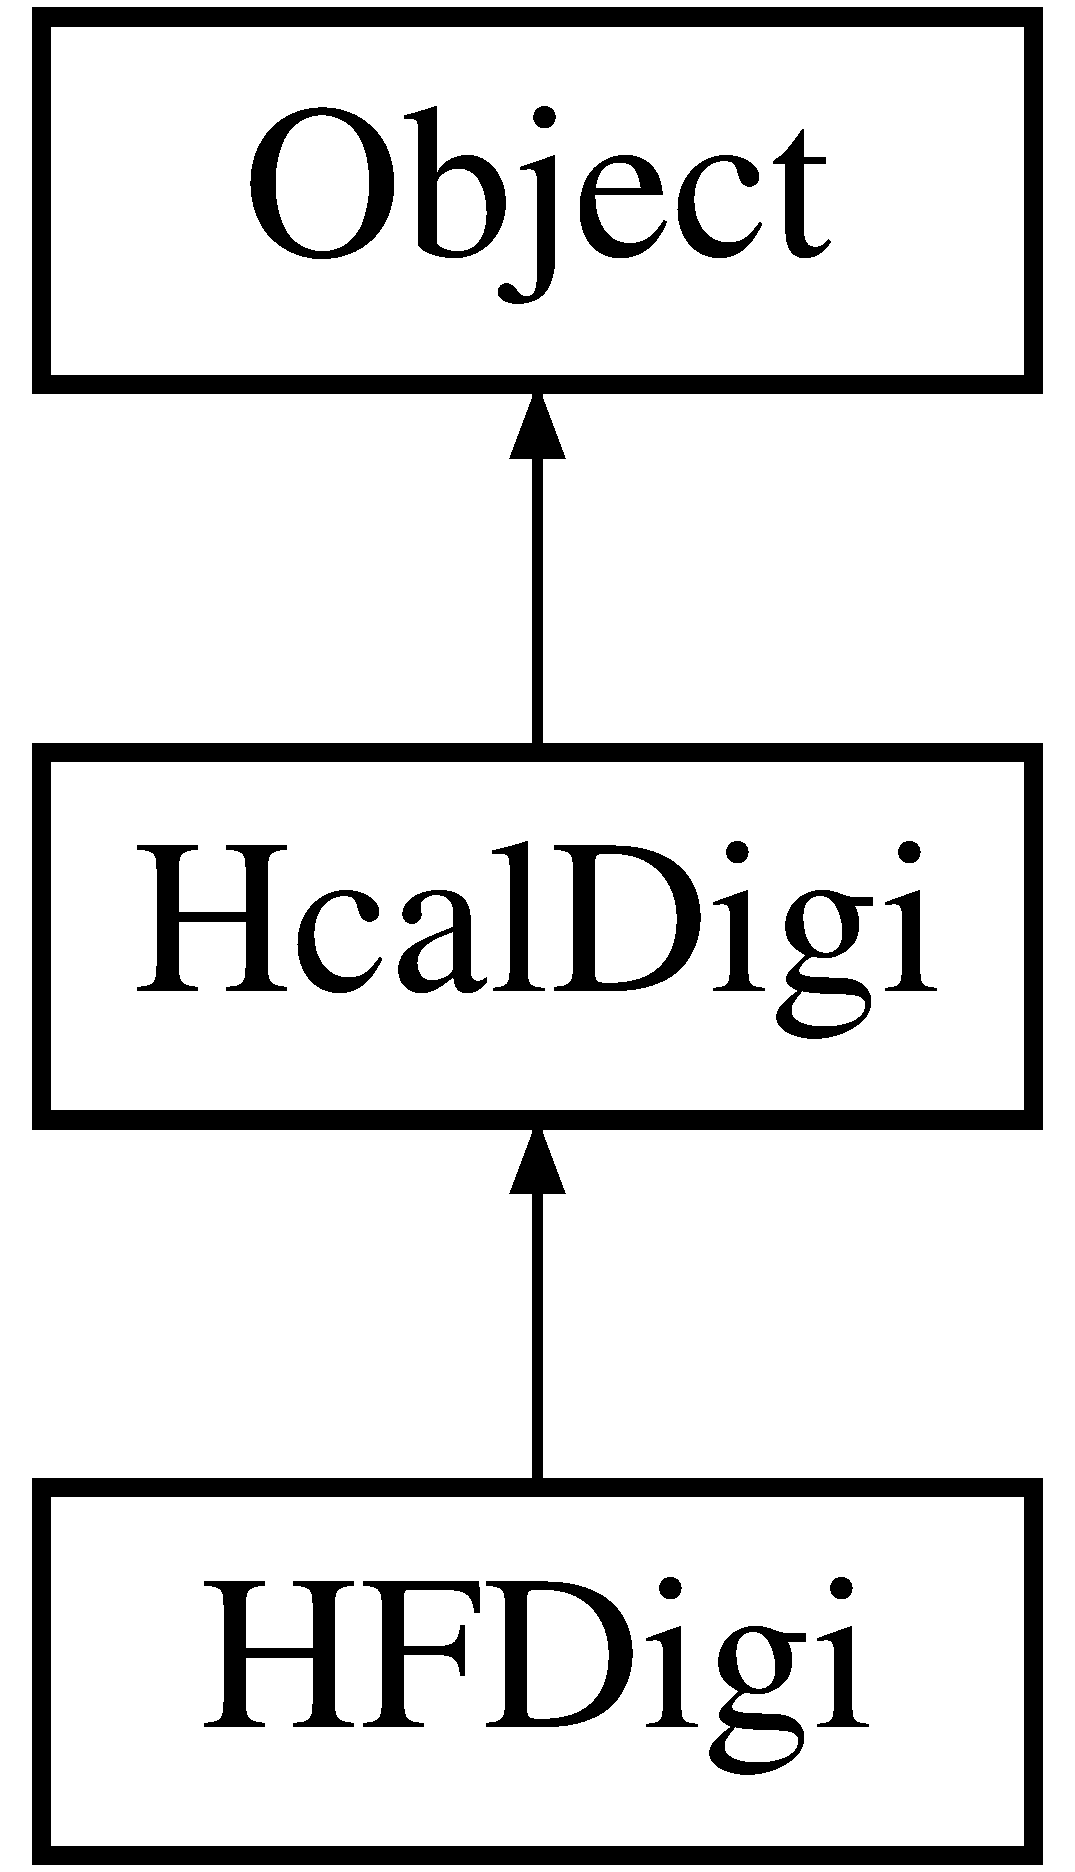
\includegraphics[height=3.000000cm]{class_h_f_digi}
\end{center}
\end{figure}
\subsection*{Public Member Functions}
\begin{DoxyCompactItemize}
\item 
\hyperlink{class_h_f_digi_a9b7e884eb5fbe2b6f093798f1f5417b3}{H\+F\+Digi} ()
\item 
\hyperlink{class_h_f_digi_af79e14f6504a822a93a70e6bffaca2ef}{H\+F\+Digi} (\hyperlink{class_collection}{Collection} \&c, unsigned short i, short j=0)
\item 
float \hyperlink{class_h_f_digi_a63778060b11696ec97f17205ea36bdb4}{energy} ()
\item 
float \hyperlink{class_h_f_digi_a04265763dd24d24360d45fa8f77ae49f}{rec\+Hit\+Time} ()
\item 
int \hyperlink{class_h_f_digi_a33b1576f22f6d8e4495944e486c6c365}{ieta} ()
\item 
int \hyperlink{class_h_f_digi_ac9d87c43f47810ff7103c51619b88cbf}{iphi} ()
\item 
int \hyperlink{class_h_f_digi_aa4f363ba278423a85893306778880db5}{depth} ()
\item 
int \hyperlink{class_h_f_digi_ad29e817757e158c1f50e4510dd31df92}{size} ()
\item 
int \hyperlink{class_h_f_digi_a33992d4a75b4545c1be9f50a6e243710}{presamples} ()
\item 
int \hyperlink{class_h_f_digi_a2d689c4c53b74e67e7a62f3a43a4f665}{electronics\+Id} ()
\item 
int \hyperlink{class_h_f_digi_a702fadfdc85d5cc5a787d9593165fb9d}{raw\+Id} ()
\item 
float \hyperlink{class_h_f_digi_aad37bf192b33e5f3e8dc0d3d1be73348}{fc} (int i)
\item 
int \hyperlink{class_h_f_digi_afd736e6e2a6292cd2e88cac49b7e919d}{adc} (int i)
\item 
int \hyperlink{class_h_f_digi_ac3e816c077f8a09a482c624352123196}{dv} (int i)
\item 
int \hyperlink{class_h_f_digi_ac648135daf87c2f957430ee50ff27fae}{er} (int i)
\item 
int \hyperlink{class_h_f_digi_a05be32bba8288c2041f49d379b66922d}{capid} (int i)
\item 
int \hyperlink{class_h_f_digi_a50c195d9ba9d66f5f80fb6896c3e176e}{get\+Raw\+Index} ()
\item 
\hyperlink{class_h_f_sample}{H\+F\+Sample} \hyperlink{class_h_f_digi_a7ce236696c1c232cc44638fb6edd5987}{operator\mbox{[}$\,$\mbox{]}} (int i)
\end{DoxyCompactItemize}
\subsection*{Additional Inherited Members}


\subsection{Constructor \& Destructor Documentation}
\hypertarget{class_h_f_digi_a9b7e884eb5fbe2b6f093798f1f5417b3}{}\index{H\+F\+Digi@{H\+F\+Digi}!H\+F\+Digi@{H\+F\+Digi}}
\index{H\+F\+Digi@{H\+F\+Digi}!H\+F\+Digi@{H\+F\+Digi}}
\subsubsection[{H\+F\+Digi()}]{\setlength{\rightskip}{0pt plus 5cm}H\+F\+Digi\+::\+H\+F\+Digi (
\begin{DoxyParamCaption}
{}
\end{DoxyParamCaption}
)}\label{class_h_f_digi_a9b7e884eb5fbe2b6f093798f1f5417b3}
\hypertarget{class_h_f_digi_af79e14f6504a822a93a70e6bffaca2ef}{}\index{H\+F\+Digi@{H\+F\+Digi}!H\+F\+Digi@{H\+F\+Digi}}
\index{H\+F\+Digi@{H\+F\+Digi}!H\+F\+Digi@{H\+F\+Digi}}
\subsubsection[{H\+F\+Digi(\+Collection \&c, unsigned short i, short j=0)}]{\setlength{\rightskip}{0pt plus 5cm}H\+F\+Digi\+::\+H\+F\+Digi (
\begin{DoxyParamCaption}
\item[{{\bf Collection} \&}]{c, }
\item[{unsigned short}]{i, }
\item[{short}]{j = {\ttfamily 0}}
\end{DoxyParamCaption}
)}\label{class_h_f_digi_af79e14f6504a822a93a70e6bffaca2ef}


\subsection{Member Function Documentation}
\hypertarget{class_h_f_digi_afd736e6e2a6292cd2e88cac49b7e919d}{}\index{H\+F\+Digi@{H\+F\+Digi}!adc@{adc}}
\index{adc@{adc}!H\+F\+Digi@{H\+F\+Digi}}
\subsubsection[{adc(int i)}]{\setlength{\rightskip}{0pt plus 5cm}int H\+F\+Digi\+::adc (
\begin{DoxyParamCaption}
\item[{int}]{i}
\end{DoxyParamCaption}
)\hspace{0.3cm}{\ttfamily [virtual]}}\label{class_h_f_digi_afd736e6e2a6292cd2e88cac49b7e919d}


Implements \hyperlink{class_hcal_digi_a737b46ab9bc5439f32232ee6911ed516}{Hcal\+Digi}.

\hypertarget{class_h_f_digi_a05be32bba8288c2041f49d379b66922d}{}\index{H\+F\+Digi@{H\+F\+Digi}!capid@{capid}}
\index{capid@{capid}!H\+F\+Digi@{H\+F\+Digi}}
\subsubsection[{capid(int i)}]{\setlength{\rightskip}{0pt plus 5cm}int H\+F\+Digi\+::capid (
\begin{DoxyParamCaption}
\item[{int}]{i}
\end{DoxyParamCaption}
)\hspace{0.3cm}{\ttfamily [virtual]}}\label{class_h_f_digi_a05be32bba8288c2041f49d379b66922d}


Implements \hyperlink{class_hcal_digi_ad6e205312dda117af660b9391d502155}{Hcal\+Digi}.

\hypertarget{class_h_f_digi_aa4f363ba278423a85893306778880db5}{}\index{H\+F\+Digi@{H\+F\+Digi}!depth@{depth}}
\index{depth@{depth}!H\+F\+Digi@{H\+F\+Digi}}
\subsubsection[{depth()}]{\setlength{\rightskip}{0pt plus 5cm}int H\+F\+Digi\+::depth (
\begin{DoxyParamCaption}
{}
\end{DoxyParamCaption}
)\hspace{0.3cm}{\ttfamily [virtual]}}\label{class_h_f_digi_aa4f363ba278423a85893306778880db5}


Implements \hyperlink{class_hcal_digi_a916a582b044a64e041ba38e545349f7f}{Hcal\+Digi}.

\hypertarget{class_h_f_digi_ac3e816c077f8a09a482c624352123196}{}\index{H\+F\+Digi@{H\+F\+Digi}!dv@{dv}}
\index{dv@{dv}!H\+F\+Digi@{H\+F\+Digi}}
\subsubsection[{dv(int i)}]{\setlength{\rightskip}{0pt plus 5cm}int H\+F\+Digi\+::dv (
\begin{DoxyParamCaption}
\item[{int}]{i}
\end{DoxyParamCaption}
)\hspace{0.3cm}{\ttfamily [virtual]}}\label{class_h_f_digi_ac3e816c077f8a09a482c624352123196}


Implements \hyperlink{class_hcal_digi_aa758519b70ab24ac4bb7635052cfa174}{Hcal\+Digi}.

\hypertarget{class_h_f_digi_a2d689c4c53b74e67e7a62f3a43a4f665}{}\index{H\+F\+Digi@{H\+F\+Digi}!electronics\+Id@{electronics\+Id}}
\index{electronics\+Id@{electronics\+Id}!H\+F\+Digi@{H\+F\+Digi}}
\subsubsection[{electronics\+Id()}]{\setlength{\rightskip}{0pt plus 5cm}int H\+F\+Digi\+::electronics\+Id (
\begin{DoxyParamCaption}
{}
\end{DoxyParamCaption}
)\hspace{0.3cm}{\ttfamily [virtual]}}\label{class_h_f_digi_a2d689c4c53b74e67e7a62f3a43a4f665}


Implements \hyperlink{class_hcal_digi_afc95a09767a731b098cb2e22b89cc4e0}{Hcal\+Digi}.

\hypertarget{class_h_f_digi_a63778060b11696ec97f17205ea36bdb4}{}\index{H\+F\+Digi@{H\+F\+Digi}!energy@{energy}}
\index{energy@{energy}!H\+F\+Digi@{H\+F\+Digi}}
\subsubsection[{energy()}]{\setlength{\rightskip}{0pt plus 5cm}float H\+F\+Digi\+::energy (
\begin{DoxyParamCaption}
{}
\end{DoxyParamCaption}
)\hspace{0.3cm}{\ttfamily [virtual]}}\label{class_h_f_digi_a63778060b11696ec97f17205ea36bdb4}


Implements \hyperlink{class_hcal_digi_a665c0fa940132fafc6dce9fd75f18cea}{Hcal\+Digi}.

\hypertarget{class_h_f_digi_ac648135daf87c2f957430ee50ff27fae}{}\index{H\+F\+Digi@{H\+F\+Digi}!er@{er}}
\index{er@{er}!H\+F\+Digi@{H\+F\+Digi}}
\subsubsection[{er(int i)}]{\setlength{\rightskip}{0pt plus 5cm}int H\+F\+Digi\+::er (
\begin{DoxyParamCaption}
\item[{int}]{i}
\end{DoxyParamCaption}
)\hspace{0.3cm}{\ttfamily [virtual]}}\label{class_h_f_digi_ac648135daf87c2f957430ee50ff27fae}


Implements \hyperlink{class_hcal_digi_a04b02a86692bcdff2fb8fa8c50cc0c34}{Hcal\+Digi}.

\hypertarget{class_h_f_digi_aad37bf192b33e5f3e8dc0d3d1be73348}{}\index{H\+F\+Digi@{H\+F\+Digi}!fc@{fc}}
\index{fc@{fc}!H\+F\+Digi@{H\+F\+Digi}}
\subsubsection[{fc(int i)}]{\setlength{\rightskip}{0pt plus 5cm}float H\+F\+Digi\+::fc (
\begin{DoxyParamCaption}
\item[{int}]{i}
\end{DoxyParamCaption}
)\hspace{0.3cm}{\ttfamily [virtual]}}\label{class_h_f_digi_aad37bf192b33e5f3e8dc0d3d1be73348}


Implements \hyperlink{class_hcal_digi_a4a5e45ca390ee81fe384bf4a7d05f1e0}{Hcal\+Digi}.

\hypertarget{class_h_f_digi_a50c195d9ba9d66f5f80fb6896c3e176e}{}\index{H\+F\+Digi@{H\+F\+Digi}!get\+Raw\+Index@{get\+Raw\+Index}}
\index{get\+Raw\+Index@{get\+Raw\+Index}!H\+F\+Digi@{H\+F\+Digi}}
\subsubsection[{get\+Raw\+Index()}]{\setlength{\rightskip}{0pt plus 5cm}int H\+F\+Digi\+::get\+Raw\+Index (
\begin{DoxyParamCaption}
{}
\end{DoxyParamCaption}
)\hspace{0.3cm}{\ttfamily [inline]}}\label{class_h_f_digi_a50c195d9ba9d66f5f80fb6896c3e176e}
\hypertarget{class_h_f_digi_a33b1576f22f6d8e4495944e486c6c365}{}\index{H\+F\+Digi@{H\+F\+Digi}!ieta@{ieta}}
\index{ieta@{ieta}!H\+F\+Digi@{H\+F\+Digi}}
\subsubsection[{ieta()}]{\setlength{\rightskip}{0pt plus 5cm}int H\+F\+Digi\+::ieta (
\begin{DoxyParamCaption}
{}
\end{DoxyParamCaption}
)\hspace{0.3cm}{\ttfamily [virtual]}}\label{class_h_f_digi_a33b1576f22f6d8e4495944e486c6c365}


Implements \hyperlink{class_hcal_digi_a65fc605c5c3bca7f78d961400d145c94}{Hcal\+Digi}.

\hypertarget{class_h_f_digi_ac9d87c43f47810ff7103c51619b88cbf}{}\index{H\+F\+Digi@{H\+F\+Digi}!iphi@{iphi}}
\index{iphi@{iphi}!H\+F\+Digi@{H\+F\+Digi}}
\subsubsection[{iphi()}]{\setlength{\rightskip}{0pt plus 5cm}int H\+F\+Digi\+::iphi (
\begin{DoxyParamCaption}
{}
\end{DoxyParamCaption}
)\hspace{0.3cm}{\ttfamily [virtual]}}\label{class_h_f_digi_ac9d87c43f47810ff7103c51619b88cbf}


Implements \hyperlink{class_hcal_digi_a979dec4585c9d07a7dc4060dfb97f089}{Hcal\+Digi}.

\hypertarget{class_h_f_digi_a7ce236696c1c232cc44638fb6edd5987}{}\index{H\+F\+Digi@{H\+F\+Digi}!operator\mbox{[}$\,$\mbox{]}@{operator[]}}
\index{operator\mbox{[}$\,$\mbox{]}@{operator[]}!H\+F\+Digi@{H\+F\+Digi}}
\subsubsection[{operator[](int i)}]{\setlength{\rightskip}{0pt plus 5cm}{\bf H\+F\+Sample} H\+F\+Digi\+::operator\mbox{[}$\,$\mbox{]} (
\begin{DoxyParamCaption}
\item[{int}]{i}
\end{DoxyParamCaption}
)\hspace{0.3cm}{\ttfamily [inline]}}\label{class_h_f_digi_a7ce236696c1c232cc44638fb6edd5987}
\hypertarget{class_h_f_digi_a33992d4a75b4545c1be9f50a6e243710}{}\index{H\+F\+Digi@{H\+F\+Digi}!presamples@{presamples}}
\index{presamples@{presamples}!H\+F\+Digi@{H\+F\+Digi}}
\subsubsection[{presamples()}]{\setlength{\rightskip}{0pt plus 5cm}int H\+F\+Digi\+::presamples (
\begin{DoxyParamCaption}
{}
\end{DoxyParamCaption}
)\hspace{0.3cm}{\ttfamily [virtual]}}\label{class_h_f_digi_a33992d4a75b4545c1be9f50a6e243710}


Implements \hyperlink{class_hcal_digi_aad0fc232379d8bdd40d6be32b3c980c4}{Hcal\+Digi}.

\hypertarget{class_h_f_digi_a702fadfdc85d5cc5a787d9593165fb9d}{}\index{H\+F\+Digi@{H\+F\+Digi}!raw\+Id@{raw\+Id}}
\index{raw\+Id@{raw\+Id}!H\+F\+Digi@{H\+F\+Digi}}
\subsubsection[{raw\+Id()}]{\setlength{\rightskip}{0pt plus 5cm}int H\+F\+Digi\+::raw\+Id (
\begin{DoxyParamCaption}
{}
\end{DoxyParamCaption}
)\hspace{0.3cm}{\ttfamily [virtual]}}\label{class_h_f_digi_a702fadfdc85d5cc5a787d9593165fb9d}


Implements \hyperlink{class_hcal_digi_aba55732d16499ad510091c769807f8e1}{Hcal\+Digi}.

\hypertarget{class_h_f_digi_a04265763dd24d24360d45fa8f77ae49f}{}\index{H\+F\+Digi@{H\+F\+Digi}!rec\+Hit\+Time@{rec\+Hit\+Time}}
\index{rec\+Hit\+Time@{rec\+Hit\+Time}!H\+F\+Digi@{H\+F\+Digi}}
\subsubsection[{rec\+Hit\+Time()}]{\setlength{\rightskip}{0pt plus 5cm}float H\+F\+Digi\+::rec\+Hit\+Time (
\begin{DoxyParamCaption}
{}
\end{DoxyParamCaption}
)\hspace{0.3cm}{\ttfamily [virtual]}}\label{class_h_f_digi_a04265763dd24d24360d45fa8f77ae49f}


Implements \hyperlink{class_hcal_digi_a3936cda623fc7535ed35d8d1c6abb350}{Hcal\+Digi}.

\hypertarget{class_h_f_digi_ad29e817757e158c1f50e4510dd31df92}{}\index{H\+F\+Digi@{H\+F\+Digi}!size@{size}}
\index{size@{size}!H\+F\+Digi@{H\+F\+Digi}}
\subsubsection[{size()}]{\setlength{\rightskip}{0pt plus 5cm}int H\+F\+Digi\+::size (
\begin{DoxyParamCaption}
{}
\end{DoxyParamCaption}
)\hspace{0.3cm}{\ttfamily [virtual]}}\label{class_h_f_digi_ad29e817757e158c1f50e4510dd31df92}


Implements \hyperlink{class_hcal_digi_a054f6f17539c8042d2900144d06eb4fc}{Hcal\+Digi}.



The documentation for this class was generated from the following files\+:\begin{DoxyCompactItemize}
\item 
interface/\hyperlink{_h_f_digi_8h}{H\+F\+Digi.\+h}\item 
src/\hyperlink{_h_f_digi_8cc}{H\+F\+Digi.\+cc}\end{DoxyCompactItemize}

\hypertarget{class_h_f_sample}{}\section{H\+F\+Sample Class Reference}
\label{class_h_f_sample}\index{H\+F\+Sample@{H\+F\+Sample}}


{\ttfamily \#include $<$H\+F\+Sample.\+h$>$}

Inheritance diagram for H\+F\+Sample\+:\begin{figure}[H]
\begin{center}
\leavevmode
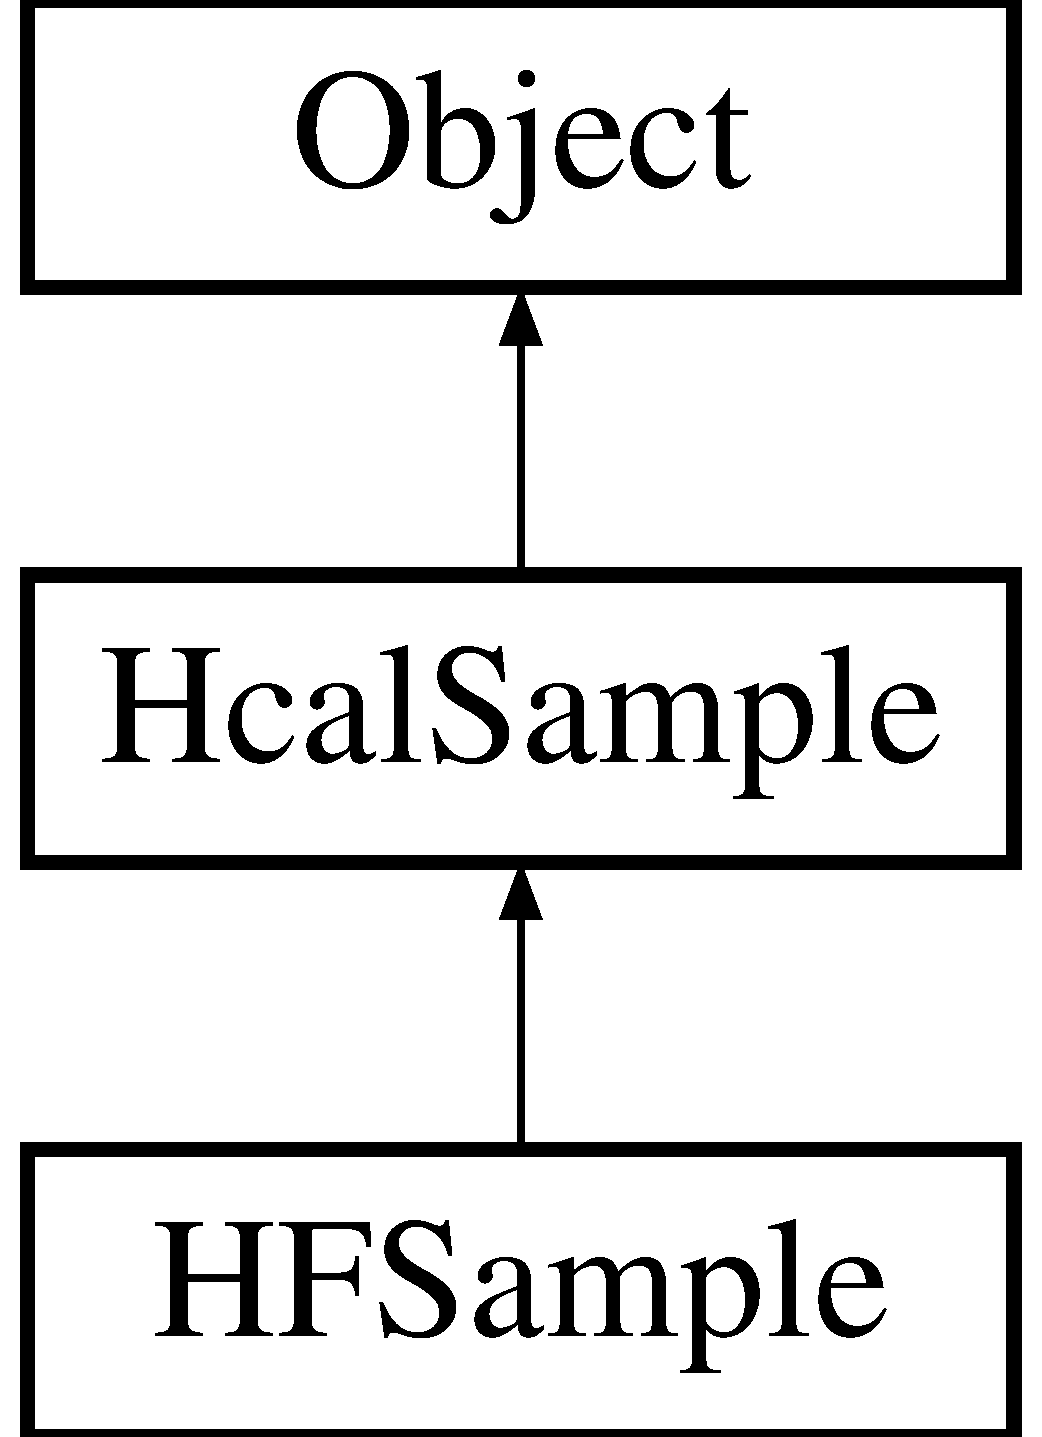
\includegraphics[height=3.000000cm]{class_h_f_sample}
\end{center}
\end{figure}
\subsection*{Public Member Functions}
\begin{DoxyCompactItemize}
\item 
\hyperlink{class_h_f_sample_a1ead2dedd8fdc3ee9259ca9ef399f9f4}{H\+F\+Sample} ()
\item 
\hyperlink{class_h_f_sample_a339037881958644ba6be17a08de2b82f}{H\+F\+Sample} (\hyperlink{class_collection}{Collection} \&c, unsigned short i, short j)
\item 
float \hyperlink{class_h_f_sample_a8903a7d7f5dcc3cfc57be371e1a61d11}{all\+F\+C} ()
\item 
float \hyperlink{class_h_f_sample_ab6021ff226750df9c11bfa8a9ae956eb}{energy} ()
\item 
float \hyperlink{class_h_f_sample_a210b2ca2173c8267e3c3ba86bcad3e96}{gain} ()
\item 
float \hyperlink{class_h_f_sample_a02a219abba2029e93e0740d966ba0caf}{fc} ()
\item 
float \hyperlink{class_h_f_sample_a4356ce2fc34149ba580f72609565f9b8}{nom\+F\+C} ()
\item 
float \hyperlink{class_h_f_sample_ad99d42390ac0646749acd988680d750d}{ped\+F\+C} ()
\item 
float \hyperlink{class_h_f_sample_aebbfa0a6e0596461bc8585551e12fd38}{rc\+Gain} ()
\item 
int \hyperlink{class_h_f_sample_a6de90bbb0f186174e2c4c8788a7f7d46}{adc} ()
\item 
int \hyperlink{class_h_f_sample_a20b55dedbf364a02ee11f63f66adad86}{capid} ()
\item 
int \hyperlink{class_h_f_sample_a57495b56198eb49caf8f34b1554969f9}{dv} ()
\item 
int \hyperlink{class_h_f_sample_a38c50f0bec2401db64258670b423acd9}{er} ()
\item 
int \hyperlink{class_h_f_sample_a048dea0ef5de5cf9904fb2397427d6f4}{fiber} ()
\item 
int \hyperlink{class_h_f_sample_a82342cdd81bc6252e8272a4ff1961d08}{fiber\+Chan} ()
\item 
int \hyperlink{class_h_f_sample_a2709fd941ccbbb029bbbbdd07ceb83f4}{raw} ()
\item 
int \hyperlink{class_h_f_sample_a10a8b486edceeb52424c4f1a6b42451c}{get\+Raw\+Index} ()
\item 
int \hyperlink{class_h_f_sample_ac1daba352bc70c63b0fb2ae8504aeed6}{get\+Time\+Slice} ()
\end{DoxyCompactItemize}
\subsection*{Additional Inherited Members}


\subsection{Constructor \& Destructor Documentation}
\hypertarget{class_h_f_sample_a1ead2dedd8fdc3ee9259ca9ef399f9f4}{}\index{H\+F\+Sample@{H\+F\+Sample}!H\+F\+Sample@{H\+F\+Sample}}
\index{H\+F\+Sample@{H\+F\+Sample}!H\+F\+Sample@{H\+F\+Sample}}
\subsubsection[{H\+F\+Sample()}]{\setlength{\rightskip}{0pt plus 5cm}H\+F\+Sample\+::\+H\+F\+Sample (
\begin{DoxyParamCaption}
{}
\end{DoxyParamCaption}
)}\label{class_h_f_sample_a1ead2dedd8fdc3ee9259ca9ef399f9f4}
\hypertarget{class_h_f_sample_a339037881958644ba6be17a08de2b82f}{}\index{H\+F\+Sample@{H\+F\+Sample}!H\+F\+Sample@{H\+F\+Sample}}
\index{H\+F\+Sample@{H\+F\+Sample}!H\+F\+Sample@{H\+F\+Sample}}
\subsubsection[{H\+F\+Sample(\+Collection \&c, unsigned short i, short j)}]{\setlength{\rightskip}{0pt plus 5cm}H\+F\+Sample\+::\+H\+F\+Sample (
\begin{DoxyParamCaption}
\item[{{\bf Collection} \&}]{c, }
\item[{unsigned short}]{i, }
\item[{short}]{j}
\end{DoxyParamCaption}
)}\label{class_h_f_sample_a339037881958644ba6be17a08de2b82f}


\subsection{Member Function Documentation}
\hypertarget{class_h_f_sample_a6de90bbb0f186174e2c4c8788a7f7d46}{}\index{H\+F\+Sample@{H\+F\+Sample}!adc@{adc}}
\index{adc@{adc}!H\+F\+Sample@{H\+F\+Sample}}
\subsubsection[{adc()}]{\setlength{\rightskip}{0pt plus 5cm}int H\+F\+Sample\+::adc (
\begin{DoxyParamCaption}
{}
\end{DoxyParamCaption}
)\hspace{0.3cm}{\ttfamily [virtual]}}\label{class_h_f_sample_a6de90bbb0f186174e2c4c8788a7f7d46}


Implements \hyperlink{class_hcal_sample_a3801777ac080ca0e512c226e4cfd5682}{Hcal\+Sample}.

\hypertarget{class_h_f_sample_a8903a7d7f5dcc3cfc57be371e1a61d11}{}\index{H\+F\+Sample@{H\+F\+Sample}!all\+F\+C@{all\+F\+C}}
\index{all\+F\+C@{all\+F\+C}!H\+F\+Sample@{H\+F\+Sample}}
\subsubsection[{all\+F\+C()}]{\setlength{\rightskip}{0pt plus 5cm}float H\+F\+Sample\+::all\+F\+C (
\begin{DoxyParamCaption}
{}
\end{DoxyParamCaption}
)\hspace{0.3cm}{\ttfamily [virtual]}}\label{class_h_f_sample_a8903a7d7f5dcc3cfc57be371e1a61d11}


Implements \hyperlink{class_hcal_sample_af837bd894eb8eae865023a526940ee15}{Hcal\+Sample}.

\hypertarget{class_h_f_sample_a20b55dedbf364a02ee11f63f66adad86}{}\index{H\+F\+Sample@{H\+F\+Sample}!capid@{capid}}
\index{capid@{capid}!H\+F\+Sample@{H\+F\+Sample}}
\subsubsection[{capid()}]{\setlength{\rightskip}{0pt plus 5cm}int H\+F\+Sample\+::capid (
\begin{DoxyParamCaption}
{}
\end{DoxyParamCaption}
)\hspace{0.3cm}{\ttfamily [virtual]}}\label{class_h_f_sample_a20b55dedbf364a02ee11f63f66adad86}


Implements \hyperlink{class_hcal_sample_a51a82042ba140a68f9659140c48d83bc}{Hcal\+Sample}.

\hypertarget{class_h_f_sample_a57495b56198eb49caf8f34b1554969f9}{}\index{H\+F\+Sample@{H\+F\+Sample}!dv@{dv}}
\index{dv@{dv}!H\+F\+Sample@{H\+F\+Sample}}
\subsubsection[{dv()}]{\setlength{\rightskip}{0pt plus 5cm}int H\+F\+Sample\+::dv (
\begin{DoxyParamCaption}
{}
\end{DoxyParamCaption}
)\hspace{0.3cm}{\ttfamily [virtual]}}\label{class_h_f_sample_a57495b56198eb49caf8f34b1554969f9}


Implements \hyperlink{class_hcal_sample_a13c0e851a42d3122c7bba32d81e31d19}{Hcal\+Sample}.

\hypertarget{class_h_f_sample_ab6021ff226750df9c11bfa8a9ae956eb}{}\index{H\+F\+Sample@{H\+F\+Sample}!energy@{energy}}
\index{energy@{energy}!H\+F\+Sample@{H\+F\+Sample}}
\subsubsection[{energy()}]{\setlength{\rightskip}{0pt plus 5cm}float H\+F\+Sample\+::energy (
\begin{DoxyParamCaption}
{}
\end{DoxyParamCaption}
)\hspace{0.3cm}{\ttfamily [virtual]}}\label{class_h_f_sample_ab6021ff226750df9c11bfa8a9ae956eb}


Implements \hyperlink{class_hcal_sample_a603c4e95d1d49db37dd00f34275fb8f3}{Hcal\+Sample}.

\hypertarget{class_h_f_sample_a38c50f0bec2401db64258670b423acd9}{}\index{H\+F\+Sample@{H\+F\+Sample}!er@{er}}
\index{er@{er}!H\+F\+Sample@{H\+F\+Sample}}
\subsubsection[{er()}]{\setlength{\rightskip}{0pt plus 5cm}int H\+F\+Sample\+::er (
\begin{DoxyParamCaption}
{}
\end{DoxyParamCaption}
)\hspace{0.3cm}{\ttfamily [virtual]}}\label{class_h_f_sample_a38c50f0bec2401db64258670b423acd9}


Implements \hyperlink{class_hcal_sample_af1805d239ccbc17a6c307d66522da618}{Hcal\+Sample}.

\hypertarget{class_h_f_sample_a02a219abba2029e93e0740d966ba0caf}{}\index{H\+F\+Sample@{H\+F\+Sample}!fc@{fc}}
\index{fc@{fc}!H\+F\+Sample@{H\+F\+Sample}}
\subsubsection[{fc()}]{\setlength{\rightskip}{0pt plus 5cm}float H\+F\+Sample\+::fc (
\begin{DoxyParamCaption}
{}
\end{DoxyParamCaption}
)\hspace{0.3cm}{\ttfamily [virtual]}}\label{class_h_f_sample_a02a219abba2029e93e0740d966ba0caf}


Implements \hyperlink{class_hcal_sample_aed932c9f932eabed9f9bc6b1a54c20dd}{Hcal\+Sample}.

\hypertarget{class_h_f_sample_a048dea0ef5de5cf9904fb2397427d6f4}{}\index{H\+F\+Sample@{H\+F\+Sample}!fiber@{fiber}}
\index{fiber@{fiber}!H\+F\+Sample@{H\+F\+Sample}}
\subsubsection[{fiber()}]{\setlength{\rightskip}{0pt plus 5cm}int H\+F\+Sample\+::fiber (
\begin{DoxyParamCaption}
{}
\end{DoxyParamCaption}
)\hspace{0.3cm}{\ttfamily [virtual]}}\label{class_h_f_sample_a048dea0ef5de5cf9904fb2397427d6f4}


Implements \hyperlink{class_hcal_sample_a5ae9a4d213b69f5ee382c7a6b31eb446}{Hcal\+Sample}.

\hypertarget{class_h_f_sample_a82342cdd81bc6252e8272a4ff1961d08}{}\index{H\+F\+Sample@{H\+F\+Sample}!fiber\+Chan@{fiber\+Chan}}
\index{fiber\+Chan@{fiber\+Chan}!H\+F\+Sample@{H\+F\+Sample}}
\subsubsection[{fiber\+Chan()}]{\setlength{\rightskip}{0pt plus 5cm}int H\+F\+Sample\+::fiber\+Chan (
\begin{DoxyParamCaption}
{}
\end{DoxyParamCaption}
)\hspace{0.3cm}{\ttfamily [virtual]}}\label{class_h_f_sample_a82342cdd81bc6252e8272a4ff1961d08}


Implements \hyperlink{class_hcal_sample_acdd36acaedfe4e1a6114e6c56d1ed996}{Hcal\+Sample}.

\hypertarget{class_h_f_sample_a210b2ca2173c8267e3c3ba86bcad3e96}{}\index{H\+F\+Sample@{H\+F\+Sample}!gain@{gain}}
\index{gain@{gain}!H\+F\+Sample@{H\+F\+Sample}}
\subsubsection[{gain()}]{\setlength{\rightskip}{0pt plus 5cm}float H\+F\+Sample\+::gain (
\begin{DoxyParamCaption}
{}
\end{DoxyParamCaption}
)\hspace{0.3cm}{\ttfamily [virtual]}}\label{class_h_f_sample_a210b2ca2173c8267e3c3ba86bcad3e96}


Implements \hyperlink{class_hcal_sample_aefc3dd058b3b178917583ca6abbf4f01}{Hcal\+Sample}.

\hypertarget{class_h_f_sample_a10a8b486edceeb52424c4f1a6b42451c}{}\index{H\+F\+Sample@{H\+F\+Sample}!get\+Raw\+Index@{get\+Raw\+Index}}
\index{get\+Raw\+Index@{get\+Raw\+Index}!H\+F\+Sample@{H\+F\+Sample}}
\subsubsection[{get\+Raw\+Index()}]{\setlength{\rightskip}{0pt plus 5cm}int H\+F\+Sample\+::get\+Raw\+Index (
\begin{DoxyParamCaption}
{}
\end{DoxyParamCaption}
)\hspace{0.3cm}{\ttfamily [inline]}}\label{class_h_f_sample_a10a8b486edceeb52424c4f1a6b42451c}
\hypertarget{class_h_f_sample_ac1daba352bc70c63b0fb2ae8504aeed6}{}\index{H\+F\+Sample@{H\+F\+Sample}!get\+Time\+Slice@{get\+Time\+Slice}}
\index{get\+Time\+Slice@{get\+Time\+Slice}!H\+F\+Sample@{H\+F\+Sample}}
\subsubsection[{get\+Time\+Slice()}]{\setlength{\rightskip}{0pt plus 5cm}int H\+F\+Sample\+::get\+Time\+Slice (
\begin{DoxyParamCaption}
{}
\end{DoxyParamCaption}
)\hspace{0.3cm}{\ttfamily [inline]}}\label{class_h_f_sample_ac1daba352bc70c63b0fb2ae8504aeed6}
\hypertarget{class_h_f_sample_a4356ce2fc34149ba580f72609565f9b8}{}\index{H\+F\+Sample@{H\+F\+Sample}!nom\+F\+C@{nom\+F\+C}}
\index{nom\+F\+C@{nom\+F\+C}!H\+F\+Sample@{H\+F\+Sample}}
\subsubsection[{nom\+F\+C()}]{\setlength{\rightskip}{0pt plus 5cm}float H\+F\+Sample\+::nom\+F\+C (
\begin{DoxyParamCaption}
{}
\end{DoxyParamCaption}
)\hspace{0.3cm}{\ttfamily [virtual]}}\label{class_h_f_sample_a4356ce2fc34149ba580f72609565f9b8}


Implements \hyperlink{class_hcal_sample_a9f47a5b867c94c97c3d553e244e7dc87}{Hcal\+Sample}.

\hypertarget{class_h_f_sample_ad99d42390ac0646749acd988680d750d}{}\index{H\+F\+Sample@{H\+F\+Sample}!ped\+F\+C@{ped\+F\+C}}
\index{ped\+F\+C@{ped\+F\+C}!H\+F\+Sample@{H\+F\+Sample}}
\subsubsection[{ped\+F\+C()}]{\setlength{\rightskip}{0pt plus 5cm}float H\+F\+Sample\+::ped\+F\+C (
\begin{DoxyParamCaption}
{}
\end{DoxyParamCaption}
)\hspace{0.3cm}{\ttfamily [virtual]}}\label{class_h_f_sample_ad99d42390ac0646749acd988680d750d}


Implements \hyperlink{class_hcal_sample_a471f7ef87944ac870ea884a0cc957744}{Hcal\+Sample}.

\hypertarget{class_h_f_sample_a2709fd941ccbbb029bbbbdd07ceb83f4}{}\index{H\+F\+Sample@{H\+F\+Sample}!raw@{raw}}
\index{raw@{raw}!H\+F\+Sample@{H\+F\+Sample}}
\subsubsection[{raw()}]{\setlength{\rightskip}{0pt plus 5cm}int H\+F\+Sample\+::raw (
\begin{DoxyParamCaption}
{}
\end{DoxyParamCaption}
)\hspace{0.3cm}{\ttfamily [virtual]}}\label{class_h_f_sample_a2709fd941ccbbb029bbbbdd07ceb83f4}


Implements \hyperlink{class_hcal_sample_a328a0f8f80a0aae47a92500297635bd6}{Hcal\+Sample}.

\hypertarget{class_h_f_sample_aebbfa0a6e0596461bc8585551e12fd38}{}\index{H\+F\+Sample@{H\+F\+Sample}!rc\+Gain@{rc\+Gain}}
\index{rc\+Gain@{rc\+Gain}!H\+F\+Sample@{H\+F\+Sample}}
\subsubsection[{rc\+Gain()}]{\setlength{\rightskip}{0pt plus 5cm}float H\+F\+Sample\+::rc\+Gain (
\begin{DoxyParamCaption}
{}
\end{DoxyParamCaption}
)\hspace{0.3cm}{\ttfamily [virtual]}}\label{class_h_f_sample_aebbfa0a6e0596461bc8585551e12fd38}


Implements \hyperlink{class_hcal_sample_a6fd32da2d5ea80154251de366f98c49c}{Hcal\+Sample}.



The documentation for this class was generated from the following files\+:\begin{DoxyCompactItemize}
\item 
interface/\hyperlink{_h_f_sample_8h}{H\+F\+Sample.\+h}\item 
src/\hyperlink{_h_f_sample_8cc}{H\+F\+Sample.\+cc}\end{DoxyCompactItemize}

\hypertarget{class_h_f_u_t_c_a}{}\section{H\+F\+U\+T\+C\+A Class Reference}
\label{class_h_f_u_t_c_a}\index{H\+F\+U\+T\+C\+A@{H\+F\+U\+T\+C\+A}}


{\ttfamily \#include $<$H\+F\+U\+T\+C\+A.\+h$>$}

Inheritance diagram for H\+F\+U\+T\+C\+A\+:\begin{figure}[H]
\begin{center}
\leavevmode
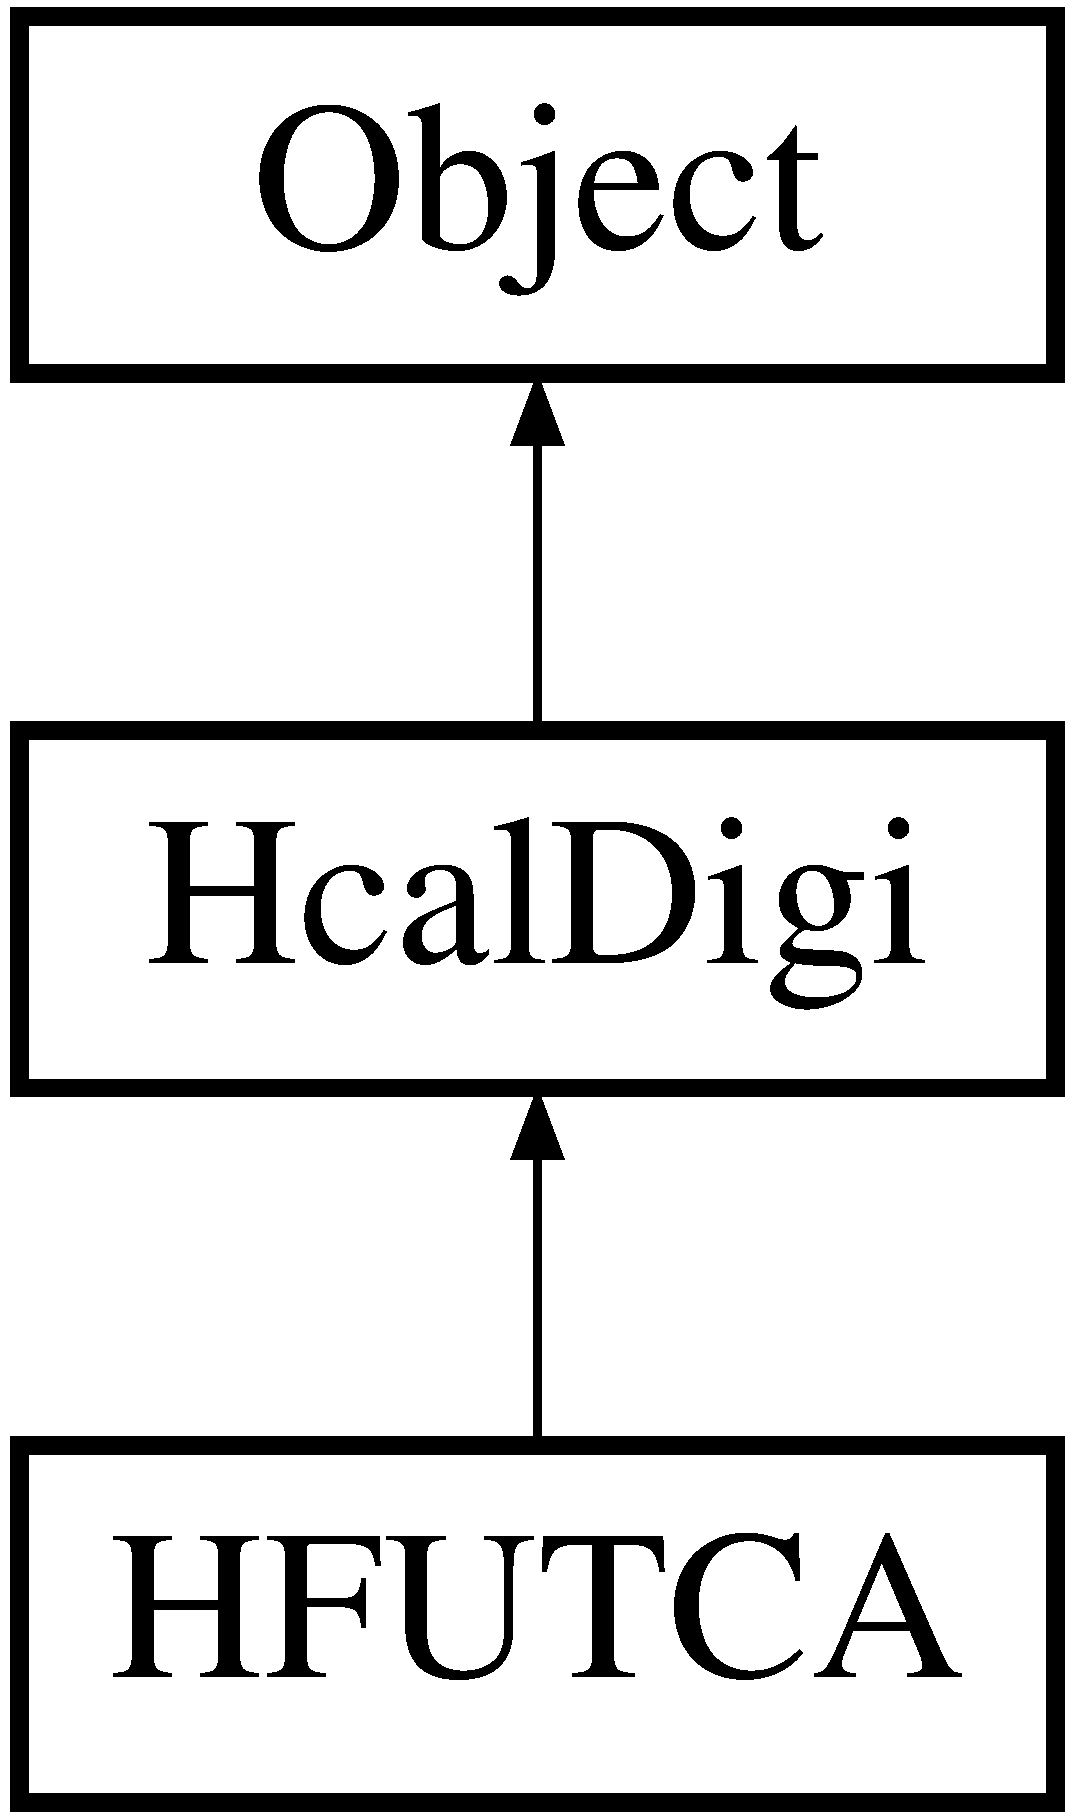
\includegraphics[height=3.000000cm]{class_h_f_u_t_c_a}
\end{center}
\end{figure}
\subsection*{Public Member Functions}
\begin{DoxyCompactItemize}
\item 
\hyperlink{class_h_f_u_t_c_a_a0cc9c566e0fa2b88ad276d11c1880ad1}{H\+F\+U\+T\+C\+A} ()
\item 
\hyperlink{class_h_f_u_t_c_a_a3125a07b0596172705e8d5def8bc8e7e}{H\+F\+U\+T\+C\+A} (\hyperlink{class_collection}{Collection} \&c, unsigned short i, short j=0)
\item 
float \hyperlink{class_h_f_u_t_c_a_adf5d3f041e1e3a43e5576b6ddcf2ad48}{energy} ()
\item 
float \hyperlink{class_h_f_u_t_c_a_a7279e3a34a60e5da92e280c4f3870cb1}{rec\+Hit\+Time} ()
\item 
int \hyperlink{class_h_f_u_t_c_a_a8a767e2e7844a50f4865041e77fbbfe1}{ieta} ()
\item 
int \hyperlink{class_h_f_u_t_c_a_ab2685221ef4d3dacbff49b066d23c662}{iphi} ()
\item 
int \hyperlink{class_h_f_u_t_c_a_a91cb1d88b08224209e156740b916ebf1}{depth} ()
\item 
int \hyperlink{class_h_f_u_t_c_a_aaecaeda5eb484331c5c8fe90fd1e94ac}{size} ()
\item 
int \hyperlink{class_h_f_u_t_c_a_a013df46d2ee37fde04c3e57fb769c248}{presamples} ()
\item 
int \hyperlink{class_h_f_u_t_c_a_a205ccadc5b455b7944b1a76d7da32d09}{raw\+Id} ()
\item 
int \hyperlink{class_h_f_u_t_c_a_abce0c33f0953b586c40e60741f8abf18}{electronics\+Id} ()
\item 
float \hyperlink{class_h_f_u_t_c_a_a71dcf59339d2814e52df6236f99d8a8c}{fc} (int i)
\item 
int \hyperlink{class_h_f_u_t_c_a_ad7540b3f782bf6fecc3d00ffd8432337}{adc} (int i)
\item 
int \hyperlink{class_h_f_u_t_c_a_a4f9ae85d537a4642d5a378c9993967c0}{dv} (int i)
\item 
int \hyperlink{class_h_f_u_t_c_a_aac6d122fbe8df975f2e4bf2dea3c4490}{er} (int i)
\item 
int \hyperlink{class_h_f_u_t_c_a_a8e7fc84c98fbce60f4a5fd5a94087ba3}{capid} (int i)
\item 
int \hyperlink{class_h_f_u_t_c_a_abb00d0d1c62b7db927d9eabb3e3543d7}{get\+Raw\+Index} ()
\item 
\hyperlink{class_h_f_u_t_c_a_sample}{H\+F\+U\+T\+C\+A\+Sample} \hyperlink{class_h_f_u_t_c_a_a9731b5cddb30d2924b16d6abd1f3a150}{operator\mbox{[}$\,$\mbox{]}} (int i)
\end{DoxyCompactItemize}
\subsection*{Additional Inherited Members}


\subsection{Constructor \& Destructor Documentation}
\hypertarget{class_h_f_u_t_c_a_a0cc9c566e0fa2b88ad276d11c1880ad1}{}\index{H\+F\+U\+T\+C\+A@{H\+F\+U\+T\+C\+A}!H\+F\+U\+T\+C\+A@{H\+F\+U\+T\+C\+A}}
\index{H\+F\+U\+T\+C\+A@{H\+F\+U\+T\+C\+A}!H\+F\+U\+T\+C\+A@{H\+F\+U\+T\+C\+A}}
\subsubsection[{H\+F\+U\+T\+C\+A()}]{\setlength{\rightskip}{0pt plus 5cm}H\+F\+U\+T\+C\+A\+::\+H\+F\+U\+T\+C\+A (
\begin{DoxyParamCaption}
{}
\end{DoxyParamCaption}
)}\label{class_h_f_u_t_c_a_a0cc9c566e0fa2b88ad276d11c1880ad1}
\hypertarget{class_h_f_u_t_c_a_a3125a07b0596172705e8d5def8bc8e7e}{}\index{H\+F\+U\+T\+C\+A@{H\+F\+U\+T\+C\+A}!H\+F\+U\+T\+C\+A@{H\+F\+U\+T\+C\+A}}
\index{H\+F\+U\+T\+C\+A@{H\+F\+U\+T\+C\+A}!H\+F\+U\+T\+C\+A@{H\+F\+U\+T\+C\+A}}
\subsubsection[{H\+F\+U\+T\+C\+A(\+Collection \&c, unsigned short i, short j=0)}]{\setlength{\rightskip}{0pt plus 5cm}H\+F\+U\+T\+C\+A\+::\+H\+F\+U\+T\+C\+A (
\begin{DoxyParamCaption}
\item[{{\bf Collection} \&}]{c, }
\item[{unsigned short}]{i, }
\item[{short}]{j = {\ttfamily 0}}
\end{DoxyParamCaption}
)}\label{class_h_f_u_t_c_a_a3125a07b0596172705e8d5def8bc8e7e}


\subsection{Member Function Documentation}
\hypertarget{class_h_f_u_t_c_a_ad7540b3f782bf6fecc3d00ffd8432337}{}\index{H\+F\+U\+T\+C\+A@{H\+F\+U\+T\+C\+A}!adc@{adc}}
\index{adc@{adc}!H\+F\+U\+T\+C\+A@{H\+F\+U\+T\+C\+A}}
\subsubsection[{adc(int i)}]{\setlength{\rightskip}{0pt plus 5cm}int H\+F\+U\+T\+C\+A\+::adc (
\begin{DoxyParamCaption}
\item[{int}]{i}
\end{DoxyParamCaption}
)\hspace{0.3cm}{\ttfamily [virtual]}}\label{class_h_f_u_t_c_a_ad7540b3f782bf6fecc3d00ffd8432337}


Implements \hyperlink{class_hcal_digi_a737b46ab9bc5439f32232ee6911ed516}{Hcal\+Digi}.

\hypertarget{class_h_f_u_t_c_a_a8e7fc84c98fbce60f4a5fd5a94087ba3}{}\index{H\+F\+U\+T\+C\+A@{H\+F\+U\+T\+C\+A}!capid@{capid}}
\index{capid@{capid}!H\+F\+U\+T\+C\+A@{H\+F\+U\+T\+C\+A}}
\subsubsection[{capid(int i)}]{\setlength{\rightskip}{0pt plus 5cm}int H\+F\+U\+T\+C\+A\+::capid (
\begin{DoxyParamCaption}
\item[{int}]{i}
\end{DoxyParamCaption}
)\hspace{0.3cm}{\ttfamily [virtual]}}\label{class_h_f_u_t_c_a_a8e7fc84c98fbce60f4a5fd5a94087ba3}


Implements \hyperlink{class_hcal_digi_ad6e205312dda117af660b9391d502155}{Hcal\+Digi}.

\hypertarget{class_h_f_u_t_c_a_a91cb1d88b08224209e156740b916ebf1}{}\index{H\+F\+U\+T\+C\+A@{H\+F\+U\+T\+C\+A}!depth@{depth}}
\index{depth@{depth}!H\+F\+U\+T\+C\+A@{H\+F\+U\+T\+C\+A}}
\subsubsection[{depth()}]{\setlength{\rightskip}{0pt plus 5cm}int H\+F\+U\+T\+C\+A\+::depth (
\begin{DoxyParamCaption}
{}
\end{DoxyParamCaption}
)\hspace{0.3cm}{\ttfamily [virtual]}}\label{class_h_f_u_t_c_a_a91cb1d88b08224209e156740b916ebf1}


Implements \hyperlink{class_hcal_digi_a916a582b044a64e041ba38e545349f7f}{Hcal\+Digi}.

\hypertarget{class_h_f_u_t_c_a_a4f9ae85d537a4642d5a378c9993967c0}{}\index{H\+F\+U\+T\+C\+A@{H\+F\+U\+T\+C\+A}!dv@{dv}}
\index{dv@{dv}!H\+F\+U\+T\+C\+A@{H\+F\+U\+T\+C\+A}}
\subsubsection[{dv(int i)}]{\setlength{\rightskip}{0pt plus 5cm}int H\+F\+U\+T\+C\+A\+::dv (
\begin{DoxyParamCaption}
\item[{int}]{i}
\end{DoxyParamCaption}
)\hspace{0.3cm}{\ttfamily [virtual]}}\label{class_h_f_u_t_c_a_a4f9ae85d537a4642d5a378c9993967c0}


Implements \hyperlink{class_hcal_digi_aa758519b70ab24ac4bb7635052cfa174}{Hcal\+Digi}.

\hypertarget{class_h_f_u_t_c_a_abce0c33f0953b586c40e60741f8abf18}{}\index{H\+F\+U\+T\+C\+A@{H\+F\+U\+T\+C\+A}!electronics\+Id@{electronics\+Id}}
\index{electronics\+Id@{electronics\+Id}!H\+F\+U\+T\+C\+A@{H\+F\+U\+T\+C\+A}}
\subsubsection[{electronics\+Id()}]{\setlength{\rightskip}{0pt plus 5cm}int H\+F\+U\+T\+C\+A\+::electronics\+Id (
\begin{DoxyParamCaption}
{}
\end{DoxyParamCaption}
)\hspace{0.3cm}{\ttfamily [virtual]}}\label{class_h_f_u_t_c_a_abce0c33f0953b586c40e60741f8abf18}


Implements \hyperlink{class_hcal_digi_afc95a09767a731b098cb2e22b89cc4e0}{Hcal\+Digi}.

\hypertarget{class_h_f_u_t_c_a_adf5d3f041e1e3a43e5576b6ddcf2ad48}{}\index{H\+F\+U\+T\+C\+A@{H\+F\+U\+T\+C\+A}!energy@{energy}}
\index{energy@{energy}!H\+F\+U\+T\+C\+A@{H\+F\+U\+T\+C\+A}}
\subsubsection[{energy()}]{\setlength{\rightskip}{0pt plus 5cm}float H\+F\+U\+T\+C\+A\+::energy (
\begin{DoxyParamCaption}
{}
\end{DoxyParamCaption}
)\hspace{0.3cm}{\ttfamily [virtual]}}\label{class_h_f_u_t_c_a_adf5d3f041e1e3a43e5576b6ddcf2ad48}


Implements \hyperlink{class_hcal_digi_a665c0fa940132fafc6dce9fd75f18cea}{Hcal\+Digi}.

\hypertarget{class_h_f_u_t_c_a_aac6d122fbe8df975f2e4bf2dea3c4490}{}\index{H\+F\+U\+T\+C\+A@{H\+F\+U\+T\+C\+A}!er@{er}}
\index{er@{er}!H\+F\+U\+T\+C\+A@{H\+F\+U\+T\+C\+A}}
\subsubsection[{er(int i)}]{\setlength{\rightskip}{0pt plus 5cm}int H\+F\+U\+T\+C\+A\+::er (
\begin{DoxyParamCaption}
\item[{int}]{i}
\end{DoxyParamCaption}
)\hspace{0.3cm}{\ttfamily [virtual]}}\label{class_h_f_u_t_c_a_aac6d122fbe8df975f2e4bf2dea3c4490}


Implements \hyperlink{class_hcal_digi_a04b02a86692bcdff2fb8fa8c50cc0c34}{Hcal\+Digi}.

\hypertarget{class_h_f_u_t_c_a_a71dcf59339d2814e52df6236f99d8a8c}{}\index{H\+F\+U\+T\+C\+A@{H\+F\+U\+T\+C\+A}!fc@{fc}}
\index{fc@{fc}!H\+F\+U\+T\+C\+A@{H\+F\+U\+T\+C\+A}}
\subsubsection[{fc(int i)}]{\setlength{\rightskip}{0pt plus 5cm}float H\+F\+U\+T\+C\+A\+::fc (
\begin{DoxyParamCaption}
\item[{int}]{i}
\end{DoxyParamCaption}
)\hspace{0.3cm}{\ttfamily [virtual]}}\label{class_h_f_u_t_c_a_a71dcf59339d2814e52df6236f99d8a8c}


Implements \hyperlink{class_hcal_digi_a4a5e45ca390ee81fe384bf4a7d05f1e0}{Hcal\+Digi}.

\hypertarget{class_h_f_u_t_c_a_abb00d0d1c62b7db927d9eabb3e3543d7}{}\index{H\+F\+U\+T\+C\+A@{H\+F\+U\+T\+C\+A}!get\+Raw\+Index@{get\+Raw\+Index}}
\index{get\+Raw\+Index@{get\+Raw\+Index}!H\+F\+U\+T\+C\+A@{H\+F\+U\+T\+C\+A}}
\subsubsection[{get\+Raw\+Index()}]{\setlength{\rightskip}{0pt plus 5cm}int H\+F\+U\+T\+C\+A\+::get\+Raw\+Index (
\begin{DoxyParamCaption}
{}
\end{DoxyParamCaption}
)\hspace{0.3cm}{\ttfamily [inline]}}\label{class_h_f_u_t_c_a_abb00d0d1c62b7db927d9eabb3e3543d7}
\hypertarget{class_h_f_u_t_c_a_a8a767e2e7844a50f4865041e77fbbfe1}{}\index{H\+F\+U\+T\+C\+A@{H\+F\+U\+T\+C\+A}!ieta@{ieta}}
\index{ieta@{ieta}!H\+F\+U\+T\+C\+A@{H\+F\+U\+T\+C\+A}}
\subsubsection[{ieta()}]{\setlength{\rightskip}{0pt plus 5cm}int H\+F\+U\+T\+C\+A\+::ieta (
\begin{DoxyParamCaption}
{}
\end{DoxyParamCaption}
)\hspace{0.3cm}{\ttfamily [virtual]}}\label{class_h_f_u_t_c_a_a8a767e2e7844a50f4865041e77fbbfe1}


Implements \hyperlink{class_hcal_digi_a65fc605c5c3bca7f78d961400d145c94}{Hcal\+Digi}.

\hypertarget{class_h_f_u_t_c_a_ab2685221ef4d3dacbff49b066d23c662}{}\index{H\+F\+U\+T\+C\+A@{H\+F\+U\+T\+C\+A}!iphi@{iphi}}
\index{iphi@{iphi}!H\+F\+U\+T\+C\+A@{H\+F\+U\+T\+C\+A}}
\subsubsection[{iphi()}]{\setlength{\rightskip}{0pt plus 5cm}int H\+F\+U\+T\+C\+A\+::iphi (
\begin{DoxyParamCaption}
{}
\end{DoxyParamCaption}
)\hspace{0.3cm}{\ttfamily [virtual]}}\label{class_h_f_u_t_c_a_ab2685221ef4d3dacbff49b066d23c662}


Implements \hyperlink{class_hcal_digi_a979dec4585c9d07a7dc4060dfb97f089}{Hcal\+Digi}.

\hypertarget{class_h_f_u_t_c_a_a9731b5cddb30d2924b16d6abd1f3a150}{}\index{H\+F\+U\+T\+C\+A@{H\+F\+U\+T\+C\+A}!operator\mbox{[}$\,$\mbox{]}@{operator[]}}
\index{operator\mbox{[}$\,$\mbox{]}@{operator[]}!H\+F\+U\+T\+C\+A@{H\+F\+U\+T\+C\+A}}
\subsubsection[{operator[](int i)}]{\setlength{\rightskip}{0pt plus 5cm}{\bf H\+F\+U\+T\+C\+A\+Sample} H\+F\+U\+T\+C\+A\+::operator\mbox{[}$\,$\mbox{]} (
\begin{DoxyParamCaption}
\item[{int}]{i}
\end{DoxyParamCaption}
)\hspace{0.3cm}{\ttfamily [inline]}}\label{class_h_f_u_t_c_a_a9731b5cddb30d2924b16d6abd1f3a150}
\hypertarget{class_h_f_u_t_c_a_a013df46d2ee37fde04c3e57fb769c248}{}\index{H\+F\+U\+T\+C\+A@{H\+F\+U\+T\+C\+A}!presamples@{presamples}}
\index{presamples@{presamples}!H\+F\+U\+T\+C\+A@{H\+F\+U\+T\+C\+A}}
\subsubsection[{presamples()}]{\setlength{\rightskip}{0pt plus 5cm}int H\+F\+U\+T\+C\+A\+::presamples (
\begin{DoxyParamCaption}
{}
\end{DoxyParamCaption}
)\hspace{0.3cm}{\ttfamily [virtual]}}\label{class_h_f_u_t_c_a_a013df46d2ee37fde04c3e57fb769c248}


Implements \hyperlink{class_hcal_digi_aad0fc232379d8bdd40d6be32b3c980c4}{Hcal\+Digi}.

\hypertarget{class_h_f_u_t_c_a_a205ccadc5b455b7944b1a76d7da32d09}{}\index{H\+F\+U\+T\+C\+A@{H\+F\+U\+T\+C\+A}!raw\+Id@{raw\+Id}}
\index{raw\+Id@{raw\+Id}!H\+F\+U\+T\+C\+A@{H\+F\+U\+T\+C\+A}}
\subsubsection[{raw\+Id()}]{\setlength{\rightskip}{0pt plus 5cm}int H\+F\+U\+T\+C\+A\+::raw\+Id (
\begin{DoxyParamCaption}
{}
\end{DoxyParamCaption}
)\hspace{0.3cm}{\ttfamily [virtual]}}\label{class_h_f_u_t_c_a_a205ccadc5b455b7944b1a76d7da32d09}


Implements \hyperlink{class_hcal_digi_aba55732d16499ad510091c769807f8e1}{Hcal\+Digi}.

\hypertarget{class_h_f_u_t_c_a_a7279e3a34a60e5da92e280c4f3870cb1}{}\index{H\+F\+U\+T\+C\+A@{H\+F\+U\+T\+C\+A}!rec\+Hit\+Time@{rec\+Hit\+Time}}
\index{rec\+Hit\+Time@{rec\+Hit\+Time}!H\+F\+U\+T\+C\+A@{H\+F\+U\+T\+C\+A}}
\subsubsection[{rec\+Hit\+Time()}]{\setlength{\rightskip}{0pt plus 5cm}float H\+F\+U\+T\+C\+A\+::rec\+Hit\+Time (
\begin{DoxyParamCaption}
{}
\end{DoxyParamCaption}
)\hspace{0.3cm}{\ttfamily [virtual]}}\label{class_h_f_u_t_c_a_a7279e3a34a60e5da92e280c4f3870cb1}


Implements \hyperlink{class_hcal_digi_a3936cda623fc7535ed35d8d1c6abb350}{Hcal\+Digi}.

\hypertarget{class_h_f_u_t_c_a_aaecaeda5eb484331c5c8fe90fd1e94ac}{}\index{H\+F\+U\+T\+C\+A@{H\+F\+U\+T\+C\+A}!size@{size}}
\index{size@{size}!H\+F\+U\+T\+C\+A@{H\+F\+U\+T\+C\+A}}
\subsubsection[{size()}]{\setlength{\rightskip}{0pt plus 5cm}int H\+F\+U\+T\+C\+A\+::size (
\begin{DoxyParamCaption}
{}
\end{DoxyParamCaption}
)\hspace{0.3cm}{\ttfamily [virtual]}}\label{class_h_f_u_t_c_a_aaecaeda5eb484331c5c8fe90fd1e94ac}


Implements \hyperlink{class_hcal_digi_a054f6f17539c8042d2900144d06eb4fc}{Hcal\+Digi}.



The documentation for this class was generated from the following file\+:\begin{DoxyCompactItemize}
\item 
interface/\hyperlink{_h_f_u_t_c_a_8h}{H\+F\+U\+T\+C\+A.\+h}\end{DoxyCompactItemize}

\hypertarget{class_h_f_u_t_c_a_sample}{}\section{H\+F\+U\+T\+C\+A\+Sample Class Reference}
\label{class_h_f_u_t_c_a_sample}\index{H\+F\+U\+T\+C\+A\+Sample@{H\+F\+U\+T\+C\+A\+Sample}}


{\ttfamily \#include $<$H\+F\+U\+T\+C\+A\+Sample.\+h$>$}

Inheritance diagram for H\+F\+U\+T\+C\+A\+Sample\+:\begin{figure}[H]
\begin{center}
\leavevmode
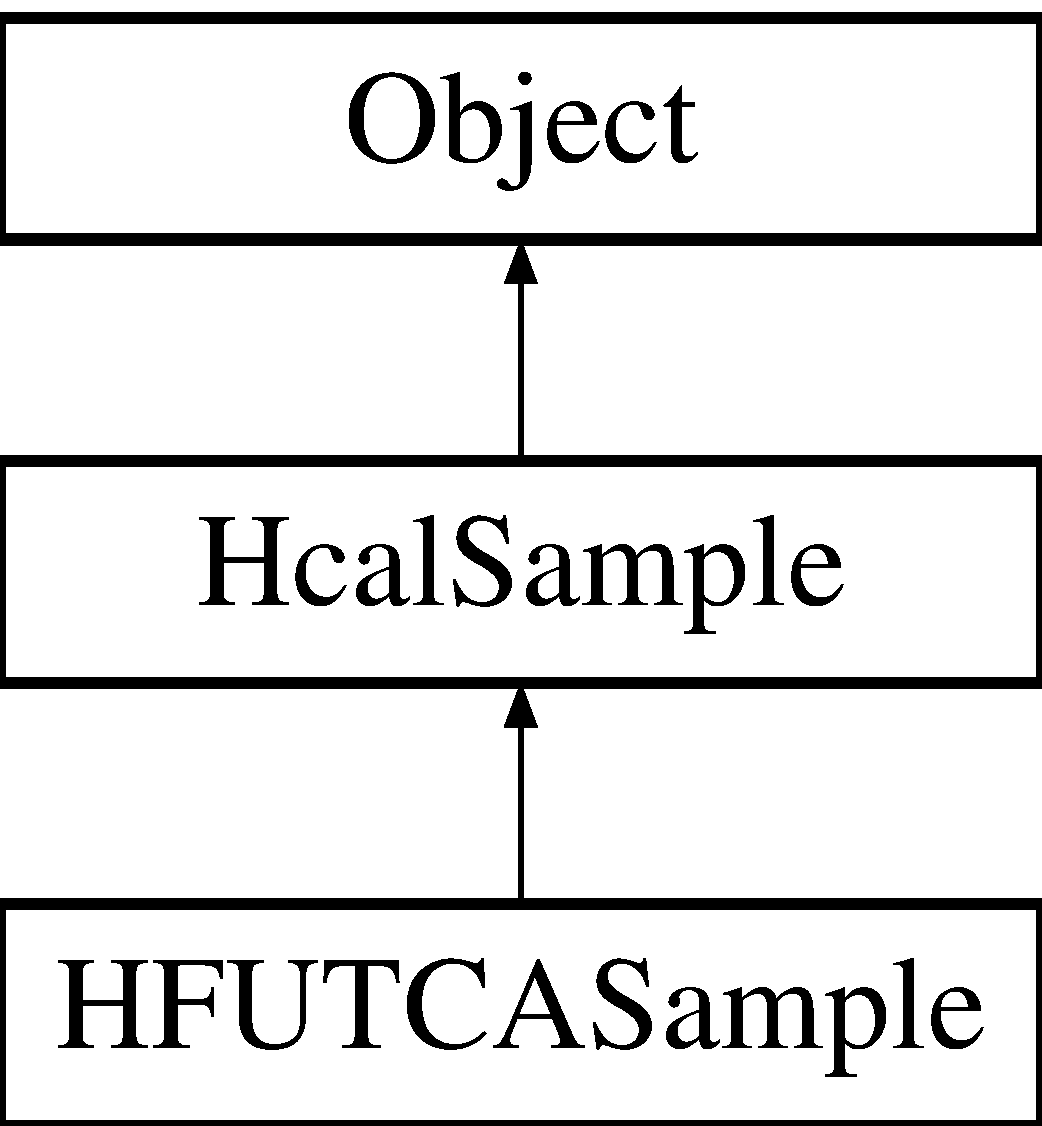
\includegraphics[height=3.000000cm]{class_h_f_u_t_c_a_sample}
\end{center}
\end{figure}
\subsection*{Public Member Functions}
\begin{DoxyCompactItemize}
\item 
\hyperlink{class_h_f_u_t_c_a_sample_a6372aa87747642e805bb705c5053b308}{H\+F\+U\+T\+C\+A\+Sample} ()
\item 
\hyperlink{class_h_f_u_t_c_a_sample_aa69d36db97b93bef64db908f0a9de2d1}{H\+F\+U\+T\+C\+A\+Sample} (\hyperlink{class_collection}{Collection} \&c, unsigned short i, short j)
\item 
float \hyperlink{class_h_f_u_t_c_a_sample_aca1a7db39701544c65d02b5b643a8752}{all\+F\+C} ()
\item 
float \hyperlink{class_h_f_u_t_c_a_sample_abd8d7c0f338668db3d18a2a79493e1ec}{energy} ()
\item 
float \hyperlink{class_h_f_u_t_c_a_sample_abda1fe3f4fd86f464fa1101469fda074}{gain} ()
\item 
float \hyperlink{class_h_f_u_t_c_a_sample_a41761d51c05dfbdf0c5da9be026dd773}{fc} ()
\item 
float \hyperlink{class_h_f_u_t_c_a_sample_a989c287e356b37be8886e93865d7a16a}{nom\+F\+C} ()
\item 
float \hyperlink{class_h_f_u_t_c_a_sample_a2bf5628c13f9908c0dc6606f2b8580c5}{ped\+F\+C} ()
\item 
float \hyperlink{class_h_f_u_t_c_a_sample_a0052d9a14ddb41b55e1e5e1983fc9684}{rc\+Gain} ()
\item 
int \hyperlink{class_h_f_u_t_c_a_sample_a6923b32caebe543bcc220c0079aaaede}{adc} ()
\item 
int \hyperlink{class_h_f_u_t_c_a_sample_ac7f68c45087e2c9d457515af56c8febc}{capid} ()
\item 
int \hyperlink{class_h_f_u_t_c_a_sample_a95f366e87ccd669a0fdb69363c71aefb}{dv} ()
\item 
int \hyperlink{class_h_f_u_t_c_a_sample_a26ede18ebc816eb8f5de7f1073566f7f}{er} ()
\item 
int \hyperlink{class_h_f_u_t_c_a_sample_aa9987206c078a46d3a41f5327c3bd83c}{fiber} ()
\item 
int \hyperlink{class_h_f_u_t_c_a_sample_acab9631919ea67506b229f7ac80a975f}{fiber\+Chan} ()
\item 
int \hyperlink{class_h_f_u_t_c_a_sample_a8aba41a05a990528d3bd3dada9e2fc91}{raw} ()
\item 
int \hyperlink{class_h_f_u_t_c_a_sample_ab9dcc1e0fa7372a4103385533267fbc5}{get\+Raw\+Index} ()
\item 
int \hyperlink{class_h_f_u_t_c_a_sample_a89c45d34d269cea4bfcfb9fb2e584151}{get\+Time\+Slice} ()
\end{DoxyCompactItemize}
\subsection*{Additional Inherited Members}


\subsection{Constructor \& Destructor Documentation}
\hypertarget{class_h_f_u_t_c_a_sample_a6372aa87747642e805bb705c5053b308}{}\index{H\+F\+U\+T\+C\+A\+Sample@{H\+F\+U\+T\+C\+A\+Sample}!H\+F\+U\+T\+C\+A\+Sample@{H\+F\+U\+T\+C\+A\+Sample}}
\index{H\+F\+U\+T\+C\+A\+Sample@{H\+F\+U\+T\+C\+A\+Sample}!H\+F\+U\+T\+C\+A\+Sample@{H\+F\+U\+T\+C\+A\+Sample}}
\subsubsection[{H\+F\+U\+T\+C\+A\+Sample()}]{\setlength{\rightskip}{0pt plus 5cm}H\+F\+U\+T\+C\+A\+Sample\+::\+H\+F\+U\+T\+C\+A\+Sample (
\begin{DoxyParamCaption}
{}
\end{DoxyParamCaption}
)}\label{class_h_f_u_t_c_a_sample_a6372aa87747642e805bb705c5053b308}
\hypertarget{class_h_f_u_t_c_a_sample_aa69d36db97b93bef64db908f0a9de2d1}{}\index{H\+F\+U\+T\+C\+A\+Sample@{H\+F\+U\+T\+C\+A\+Sample}!H\+F\+U\+T\+C\+A\+Sample@{H\+F\+U\+T\+C\+A\+Sample}}
\index{H\+F\+U\+T\+C\+A\+Sample@{H\+F\+U\+T\+C\+A\+Sample}!H\+F\+U\+T\+C\+A\+Sample@{H\+F\+U\+T\+C\+A\+Sample}}
\subsubsection[{H\+F\+U\+T\+C\+A\+Sample(\+Collection \&c, unsigned short i, short j)}]{\setlength{\rightskip}{0pt plus 5cm}H\+F\+U\+T\+C\+A\+Sample\+::\+H\+F\+U\+T\+C\+A\+Sample (
\begin{DoxyParamCaption}
\item[{{\bf Collection} \&}]{c, }
\item[{unsigned short}]{i, }
\item[{short}]{j}
\end{DoxyParamCaption}
)}\label{class_h_f_u_t_c_a_sample_aa69d36db97b93bef64db908f0a9de2d1}


\subsection{Member Function Documentation}
\hypertarget{class_h_f_u_t_c_a_sample_a6923b32caebe543bcc220c0079aaaede}{}\index{H\+F\+U\+T\+C\+A\+Sample@{H\+F\+U\+T\+C\+A\+Sample}!adc@{adc}}
\index{adc@{adc}!H\+F\+U\+T\+C\+A\+Sample@{H\+F\+U\+T\+C\+A\+Sample}}
\subsubsection[{adc()}]{\setlength{\rightskip}{0pt plus 5cm}int H\+F\+U\+T\+C\+A\+Sample\+::adc (
\begin{DoxyParamCaption}
{}
\end{DoxyParamCaption}
)\hspace{0.3cm}{\ttfamily [virtual]}}\label{class_h_f_u_t_c_a_sample_a6923b32caebe543bcc220c0079aaaede}


Implements \hyperlink{class_hcal_sample_a3801777ac080ca0e512c226e4cfd5682}{Hcal\+Sample}.

\hypertarget{class_h_f_u_t_c_a_sample_aca1a7db39701544c65d02b5b643a8752}{}\index{H\+F\+U\+T\+C\+A\+Sample@{H\+F\+U\+T\+C\+A\+Sample}!all\+F\+C@{all\+F\+C}}
\index{all\+F\+C@{all\+F\+C}!H\+F\+U\+T\+C\+A\+Sample@{H\+F\+U\+T\+C\+A\+Sample}}
\subsubsection[{all\+F\+C()}]{\setlength{\rightskip}{0pt plus 5cm}float H\+F\+U\+T\+C\+A\+Sample\+::all\+F\+C (
\begin{DoxyParamCaption}
{}
\end{DoxyParamCaption}
)\hspace{0.3cm}{\ttfamily [virtual]}}\label{class_h_f_u_t_c_a_sample_aca1a7db39701544c65d02b5b643a8752}


Implements \hyperlink{class_hcal_sample_af837bd894eb8eae865023a526940ee15}{Hcal\+Sample}.

\hypertarget{class_h_f_u_t_c_a_sample_ac7f68c45087e2c9d457515af56c8febc}{}\index{H\+F\+U\+T\+C\+A\+Sample@{H\+F\+U\+T\+C\+A\+Sample}!capid@{capid}}
\index{capid@{capid}!H\+F\+U\+T\+C\+A\+Sample@{H\+F\+U\+T\+C\+A\+Sample}}
\subsubsection[{capid()}]{\setlength{\rightskip}{0pt plus 5cm}int H\+F\+U\+T\+C\+A\+Sample\+::capid (
\begin{DoxyParamCaption}
{}
\end{DoxyParamCaption}
)\hspace{0.3cm}{\ttfamily [virtual]}}\label{class_h_f_u_t_c_a_sample_ac7f68c45087e2c9d457515af56c8febc}


Implements \hyperlink{class_hcal_sample_a51a82042ba140a68f9659140c48d83bc}{Hcal\+Sample}.

\hypertarget{class_h_f_u_t_c_a_sample_a95f366e87ccd669a0fdb69363c71aefb}{}\index{H\+F\+U\+T\+C\+A\+Sample@{H\+F\+U\+T\+C\+A\+Sample}!dv@{dv}}
\index{dv@{dv}!H\+F\+U\+T\+C\+A\+Sample@{H\+F\+U\+T\+C\+A\+Sample}}
\subsubsection[{dv()}]{\setlength{\rightskip}{0pt plus 5cm}int H\+F\+U\+T\+C\+A\+Sample\+::dv (
\begin{DoxyParamCaption}
{}
\end{DoxyParamCaption}
)\hspace{0.3cm}{\ttfamily [virtual]}}\label{class_h_f_u_t_c_a_sample_a95f366e87ccd669a0fdb69363c71aefb}


Implements \hyperlink{class_hcal_sample_a13c0e851a42d3122c7bba32d81e31d19}{Hcal\+Sample}.

\hypertarget{class_h_f_u_t_c_a_sample_abd8d7c0f338668db3d18a2a79493e1ec}{}\index{H\+F\+U\+T\+C\+A\+Sample@{H\+F\+U\+T\+C\+A\+Sample}!energy@{energy}}
\index{energy@{energy}!H\+F\+U\+T\+C\+A\+Sample@{H\+F\+U\+T\+C\+A\+Sample}}
\subsubsection[{energy()}]{\setlength{\rightskip}{0pt plus 5cm}float H\+F\+U\+T\+C\+A\+Sample\+::energy (
\begin{DoxyParamCaption}
{}
\end{DoxyParamCaption}
)\hspace{0.3cm}{\ttfamily [virtual]}}\label{class_h_f_u_t_c_a_sample_abd8d7c0f338668db3d18a2a79493e1ec}


Implements \hyperlink{class_hcal_sample_a603c4e95d1d49db37dd00f34275fb8f3}{Hcal\+Sample}.

\hypertarget{class_h_f_u_t_c_a_sample_a26ede18ebc816eb8f5de7f1073566f7f}{}\index{H\+F\+U\+T\+C\+A\+Sample@{H\+F\+U\+T\+C\+A\+Sample}!er@{er}}
\index{er@{er}!H\+F\+U\+T\+C\+A\+Sample@{H\+F\+U\+T\+C\+A\+Sample}}
\subsubsection[{er()}]{\setlength{\rightskip}{0pt plus 5cm}int H\+F\+U\+T\+C\+A\+Sample\+::er (
\begin{DoxyParamCaption}
{}
\end{DoxyParamCaption}
)\hspace{0.3cm}{\ttfamily [virtual]}}\label{class_h_f_u_t_c_a_sample_a26ede18ebc816eb8f5de7f1073566f7f}


Implements \hyperlink{class_hcal_sample_af1805d239ccbc17a6c307d66522da618}{Hcal\+Sample}.

\hypertarget{class_h_f_u_t_c_a_sample_a41761d51c05dfbdf0c5da9be026dd773}{}\index{H\+F\+U\+T\+C\+A\+Sample@{H\+F\+U\+T\+C\+A\+Sample}!fc@{fc}}
\index{fc@{fc}!H\+F\+U\+T\+C\+A\+Sample@{H\+F\+U\+T\+C\+A\+Sample}}
\subsubsection[{fc()}]{\setlength{\rightskip}{0pt plus 5cm}float H\+F\+U\+T\+C\+A\+Sample\+::fc (
\begin{DoxyParamCaption}
{}
\end{DoxyParamCaption}
)\hspace{0.3cm}{\ttfamily [virtual]}}\label{class_h_f_u_t_c_a_sample_a41761d51c05dfbdf0c5da9be026dd773}


Implements \hyperlink{class_hcal_sample_aed932c9f932eabed9f9bc6b1a54c20dd}{Hcal\+Sample}.

\hypertarget{class_h_f_u_t_c_a_sample_aa9987206c078a46d3a41f5327c3bd83c}{}\index{H\+F\+U\+T\+C\+A\+Sample@{H\+F\+U\+T\+C\+A\+Sample}!fiber@{fiber}}
\index{fiber@{fiber}!H\+F\+U\+T\+C\+A\+Sample@{H\+F\+U\+T\+C\+A\+Sample}}
\subsubsection[{fiber()}]{\setlength{\rightskip}{0pt plus 5cm}int H\+F\+U\+T\+C\+A\+Sample\+::fiber (
\begin{DoxyParamCaption}
{}
\end{DoxyParamCaption}
)\hspace{0.3cm}{\ttfamily [virtual]}}\label{class_h_f_u_t_c_a_sample_aa9987206c078a46d3a41f5327c3bd83c}


Implements \hyperlink{class_hcal_sample_a5ae9a4d213b69f5ee382c7a6b31eb446}{Hcal\+Sample}.

\hypertarget{class_h_f_u_t_c_a_sample_acab9631919ea67506b229f7ac80a975f}{}\index{H\+F\+U\+T\+C\+A\+Sample@{H\+F\+U\+T\+C\+A\+Sample}!fiber\+Chan@{fiber\+Chan}}
\index{fiber\+Chan@{fiber\+Chan}!H\+F\+U\+T\+C\+A\+Sample@{H\+F\+U\+T\+C\+A\+Sample}}
\subsubsection[{fiber\+Chan()}]{\setlength{\rightskip}{0pt plus 5cm}int H\+F\+U\+T\+C\+A\+Sample\+::fiber\+Chan (
\begin{DoxyParamCaption}
{}
\end{DoxyParamCaption}
)\hspace{0.3cm}{\ttfamily [virtual]}}\label{class_h_f_u_t_c_a_sample_acab9631919ea67506b229f7ac80a975f}


Implements \hyperlink{class_hcal_sample_acdd36acaedfe4e1a6114e6c56d1ed996}{Hcal\+Sample}.

\hypertarget{class_h_f_u_t_c_a_sample_abda1fe3f4fd86f464fa1101469fda074}{}\index{H\+F\+U\+T\+C\+A\+Sample@{H\+F\+U\+T\+C\+A\+Sample}!gain@{gain}}
\index{gain@{gain}!H\+F\+U\+T\+C\+A\+Sample@{H\+F\+U\+T\+C\+A\+Sample}}
\subsubsection[{gain()}]{\setlength{\rightskip}{0pt plus 5cm}float H\+F\+U\+T\+C\+A\+Sample\+::gain (
\begin{DoxyParamCaption}
{}
\end{DoxyParamCaption}
)\hspace{0.3cm}{\ttfamily [virtual]}}\label{class_h_f_u_t_c_a_sample_abda1fe3f4fd86f464fa1101469fda074}


Implements \hyperlink{class_hcal_sample_aefc3dd058b3b178917583ca6abbf4f01}{Hcal\+Sample}.

\hypertarget{class_h_f_u_t_c_a_sample_ab9dcc1e0fa7372a4103385533267fbc5}{}\index{H\+F\+U\+T\+C\+A\+Sample@{H\+F\+U\+T\+C\+A\+Sample}!get\+Raw\+Index@{get\+Raw\+Index}}
\index{get\+Raw\+Index@{get\+Raw\+Index}!H\+F\+U\+T\+C\+A\+Sample@{H\+F\+U\+T\+C\+A\+Sample}}
\subsubsection[{get\+Raw\+Index()}]{\setlength{\rightskip}{0pt plus 5cm}int H\+F\+U\+T\+C\+A\+Sample\+::get\+Raw\+Index (
\begin{DoxyParamCaption}
{}
\end{DoxyParamCaption}
)\hspace{0.3cm}{\ttfamily [inline]}}\label{class_h_f_u_t_c_a_sample_ab9dcc1e0fa7372a4103385533267fbc5}
\hypertarget{class_h_f_u_t_c_a_sample_a89c45d34d269cea4bfcfb9fb2e584151}{}\index{H\+F\+U\+T\+C\+A\+Sample@{H\+F\+U\+T\+C\+A\+Sample}!get\+Time\+Slice@{get\+Time\+Slice}}
\index{get\+Time\+Slice@{get\+Time\+Slice}!H\+F\+U\+T\+C\+A\+Sample@{H\+F\+U\+T\+C\+A\+Sample}}
\subsubsection[{get\+Time\+Slice()}]{\setlength{\rightskip}{0pt plus 5cm}int H\+F\+U\+T\+C\+A\+Sample\+::get\+Time\+Slice (
\begin{DoxyParamCaption}
{}
\end{DoxyParamCaption}
)\hspace{0.3cm}{\ttfamily [inline]}}\label{class_h_f_u_t_c_a_sample_a89c45d34d269cea4bfcfb9fb2e584151}
\hypertarget{class_h_f_u_t_c_a_sample_a989c287e356b37be8886e93865d7a16a}{}\index{H\+F\+U\+T\+C\+A\+Sample@{H\+F\+U\+T\+C\+A\+Sample}!nom\+F\+C@{nom\+F\+C}}
\index{nom\+F\+C@{nom\+F\+C}!H\+F\+U\+T\+C\+A\+Sample@{H\+F\+U\+T\+C\+A\+Sample}}
\subsubsection[{nom\+F\+C()}]{\setlength{\rightskip}{0pt plus 5cm}float H\+F\+U\+T\+C\+A\+Sample\+::nom\+F\+C (
\begin{DoxyParamCaption}
{}
\end{DoxyParamCaption}
)\hspace{0.3cm}{\ttfamily [virtual]}}\label{class_h_f_u_t_c_a_sample_a989c287e356b37be8886e93865d7a16a}


Implements \hyperlink{class_hcal_sample_a9f47a5b867c94c97c3d553e244e7dc87}{Hcal\+Sample}.

\hypertarget{class_h_f_u_t_c_a_sample_a2bf5628c13f9908c0dc6606f2b8580c5}{}\index{H\+F\+U\+T\+C\+A\+Sample@{H\+F\+U\+T\+C\+A\+Sample}!ped\+F\+C@{ped\+F\+C}}
\index{ped\+F\+C@{ped\+F\+C}!H\+F\+U\+T\+C\+A\+Sample@{H\+F\+U\+T\+C\+A\+Sample}}
\subsubsection[{ped\+F\+C()}]{\setlength{\rightskip}{0pt plus 5cm}float H\+F\+U\+T\+C\+A\+Sample\+::ped\+F\+C (
\begin{DoxyParamCaption}
{}
\end{DoxyParamCaption}
)\hspace{0.3cm}{\ttfamily [virtual]}}\label{class_h_f_u_t_c_a_sample_a2bf5628c13f9908c0dc6606f2b8580c5}


Implements \hyperlink{class_hcal_sample_a471f7ef87944ac870ea884a0cc957744}{Hcal\+Sample}.

\hypertarget{class_h_f_u_t_c_a_sample_a8aba41a05a990528d3bd3dada9e2fc91}{}\index{H\+F\+U\+T\+C\+A\+Sample@{H\+F\+U\+T\+C\+A\+Sample}!raw@{raw}}
\index{raw@{raw}!H\+F\+U\+T\+C\+A\+Sample@{H\+F\+U\+T\+C\+A\+Sample}}
\subsubsection[{raw()}]{\setlength{\rightskip}{0pt plus 5cm}int H\+F\+U\+T\+C\+A\+Sample\+::raw (
\begin{DoxyParamCaption}
{}
\end{DoxyParamCaption}
)\hspace{0.3cm}{\ttfamily [virtual]}}\label{class_h_f_u_t_c_a_sample_a8aba41a05a990528d3bd3dada9e2fc91}


Implements \hyperlink{class_hcal_sample_a328a0f8f80a0aae47a92500297635bd6}{Hcal\+Sample}.

\hypertarget{class_h_f_u_t_c_a_sample_a0052d9a14ddb41b55e1e5e1983fc9684}{}\index{H\+F\+U\+T\+C\+A\+Sample@{H\+F\+U\+T\+C\+A\+Sample}!rc\+Gain@{rc\+Gain}}
\index{rc\+Gain@{rc\+Gain}!H\+F\+U\+T\+C\+A\+Sample@{H\+F\+U\+T\+C\+A\+Sample}}
\subsubsection[{rc\+Gain()}]{\setlength{\rightskip}{0pt plus 5cm}float H\+F\+U\+T\+C\+A\+Sample\+::rc\+Gain (
\begin{DoxyParamCaption}
{}
\end{DoxyParamCaption}
)\hspace{0.3cm}{\ttfamily [virtual]}}\label{class_h_f_u_t_c_a_sample_a0052d9a14ddb41b55e1e5e1983fc9684}


Implements \hyperlink{class_hcal_sample_a6fd32da2d5ea80154251de366f98c49c}{Hcal\+Sample}.



The documentation for this class was generated from the following file\+:\begin{DoxyCompactItemize}
\item 
interface/\hyperlink{_h_f_u_t_c_a_sample_8h}{H\+F\+U\+T\+C\+A\+Sample.\+h}\end{DoxyCompactItemize}

\hypertarget{class_h_l_t_filter_object}{}\section{H\+L\+T\+Filter\+Object Class Reference}
\label{class_h_l_t_filter_object}\index{H\+L\+T\+Filter\+Object@{H\+L\+T\+Filter\+Object}}


{\ttfamily \#include $<$H\+L\+T\+Filter\+Object.\+h$>$}

Inheritance diagram for H\+L\+T\+Filter\+Object\+:\begin{figure}[H]
\begin{center}
\leavevmode
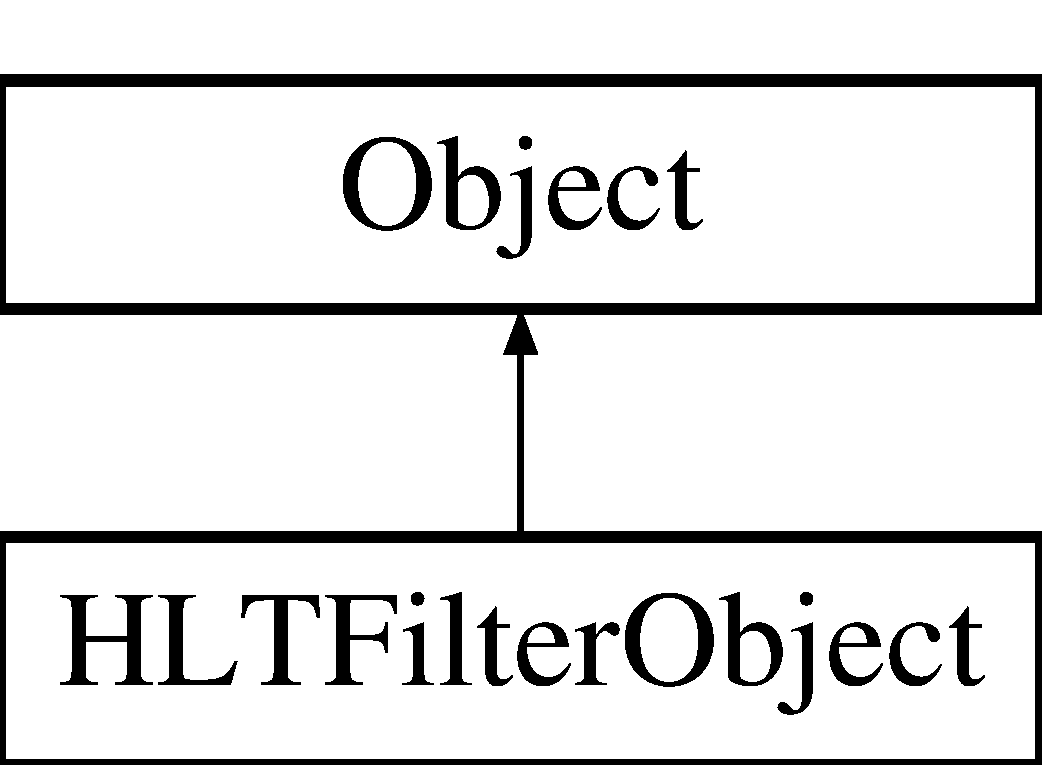
\includegraphics[height=2.000000cm]{class_h_l_t_filter_object}
\end{center}
\end{figure}
\subsection*{Public Member Functions}
\begin{DoxyCompactItemize}
\item 
\hyperlink{class_h_l_t_filter_object_a2546f99bd521875c44688d2ba97430ce}{H\+L\+T\+Filter\+Object} ()
\item 
\hyperlink{class_h_l_t_filter_object_a808d2e40a6e569a823bd7b9045ab80b1}{H\+L\+T\+Filter\+Object} (\hyperlink{class_collection}{Collection} \&collection, unsigned int index, int unsigned hlt\+\_\+filter\+\_\+index=0)
\item 
void \hyperlink{class_h_l_t_filter_object_a9d7acc3a76a2ce737dea1621027ff12c}{Write\+Pt\+Eta\+Phi} ()
\item 
double \& \hyperlink{class_h_l_t_filter_object_a29c406ea1c2dba2eca9faf17d0bb5f4e}{Pt} ()
\item 
double \& \hyperlink{class_h_l_t_filter_object_ade8858903109a380c3283b6e4203630b}{Eta} ()
\item 
double \& \hyperlink{class_h_l_t_filter_object_ae0928b247a39fa2b238312696704e370}{Phi} ()
\item 
bool \hyperlink{class_h_l_t_filter_object_a19346504ef5d039ff4032581ccccf604}{Pass\+User\+I\+D} (\hyperlink{_i_d_types_8h_a094c367727273b4da2b960ca3b3edc06}{I\+D} id, bool verbose=false)
\item 
int \hyperlink{class_h_l_t_filter_object_ac50d370e4de054e32ef3bd82f0be8e74}{Object\+I\+D} ()
\end{DoxyCompactItemize}
\subsection*{Additional Inherited Members}


\subsection{Constructor \& Destructor Documentation}
\hypertarget{class_h_l_t_filter_object_a2546f99bd521875c44688d2ba97430ce}{}\index{H\+L\+T\+Filter\+Object@{H\+L\+T\+Filter\+Object}!H\+L\+T\+Filter\+Object@{H\+L\+T\+Filter\+Object}}
\index{H\+L\+T\+Filter\+Object@{H\+L\+T\+Filter\+Object}!H\+L\+T\+Filter\+Object@{H\+L\+T\+Filter\+Object}}
\subsubsection[{H\+L\+T\+Filter\+Object()}]{\setlength{\rightskip}{0pt plus 5cm}H\+L\+T\+Filter\+Object\+::\+H\+L\+T\+Filter\+Object (
\begin{DoxyParamCaption}
{}
\end{DoxyParamCaption}
)}\label{class_h_l_t_filter_object_a2546f99bd521875c44688d2ba97430ce}
\hypertarget{class_h_l_t_filter_object_a808d2e40a6e569a823bd7b9045ab80b1}{}\index{H\+L\+T\+Filter\+Object@{H\+L\+T\+Filter\+Object}!H\+L\+T\+Filter\+Object@{H\+L\+T\+Filter\+Object}}
\index{H\+L\+T\+Filter\+Object@{H\+L\+T\+Filter\+Object}!H\+L\+T\+Filter\+Object@{H\+L\+T\+Filter\+Object}}
\subsubsection[{H\+L\+T\+Filter\+Object(\+Collection \&collection, unsigned int index, int unsigned hlt\+\_\+filter\+\_\+index=0)}]{\setlength{\rightskip}{0pt plus 5cm}H\+L\+T\+Filter\+Object\+::\+H\+L\+T\+Filter\+Object (
\begin{DoxyParamCaption}
\item[{{\bf Collection} \&}]{collection, }
\item[{unsigned int}]{index, }
\item[{int unsigned}]{hlt\+\_\+filter\+\_\+index = {\ttfamily 0}}
\end{DoxyParamCaption}
)}\label{class_h_l_t_filter_object_a808d2e40a6e569a823bd7b9045ab80b1}


\subsection{Member Function Documentation}
\hypertarget{class_h_l_t_filter_object_ade8858903109a380c3283b6e4203630b}{}\index{H\+L\+T\+Filter\+Object@{H\+L\+T\+Filter\+Object}!Eta@{Eta}}
\index{Eta@{Eta}!H\+L\+T\+Filter\+Object@{H\+L\+T\+Filter\+Object}}
\subsubsection[{Eta()}]{\setlength{\rightskip}{0pt plus 5cm}double\& H\+L\+T\+Filter\+Object\+::\+Eta (
\begin{DoxyParamCaption}
{}
\end{DoxyParamCaption}
)\hspace{0.3cm}{\ttfamily [virtual]}}\label{class_h_l_t_filter_object_ade8858903109a380c3283b6e4203630b}


Implements \hyperlink{class_object_a3760d2b4b0723118234370675654d46a}{Object}.

\hypertarget{class_h_l_t_filter_object_ac50d370e4de054e32ef3bd82f0be8e74}{}\index{H\+L\+T\+Filter\+Object@{H\+L\+T\+Filter\+Object}!Object\+I\+D@{Object\+I\+D}}
\index{Object\+I\+D@{Object\+I\+D}!H\+L\+T\+Filter\+Object@{H\+L\+T\+Filter\+Object}}
\subsubsection[{Object\+I\+D()}]{\setlength{\rightskip}{0pt plus 5cm}int H\+L\+T\+Filter\+Object\+::\+Object\+I\+D (
\begin{DoxyParamCaption}
{}
\end{DoxyParamCaption}
)}\label{class_h_l_t_filter_object_ac50d370e4de054e32ef3bd82f0be8e74}
\hypertarget{class_h_l_t_filter_object_a19346504ef5d039ff4032581ccccf604}{}\index{H\+L\+T\+Filter\+Object@{H\+L\+T\+Filter\+Object}!Pass\+User\+I\+D@{Pass\+User\+I\+D}}
\index{Pass\+User\+I\+D@{Pass\+User\+I\+D}!H\+L\+T\+Filter\+Object@{H\+L\+T\+Filter\+Object}}
\subsubsection[{Pass\+User\+I\+D(\+I\+D id, bool verbose=false)}]{\setlength{\rightskip}{0pt plus 5cm}bool H\+L\+T\+Filter\+Object\+::\+Pass\+User\+I\+D (
\begin{DoxyParamCaption}
\item[{{\bf I\+D}}]{id, }
\item[{bool}]{verbose = {\ttfamily false}}
\end{DoxyParamCaption}
)\hspace{0.3cm}{\ttfamily [virtual]}}\label{class_h_l_t_filter_object_a19346504ef5d039ff4032581ccccf604}


Implements \hyperlink{class_object_ae28bc9879447dad23f10ebd1971e81f5}{Object}.

\hypertarget{class_h_l_t_filter_object_ae0928b247a39fa2b238312696704e370}{}\index{H\+L\+T\+Filter\+Object@{H\+L\+T\+Filter\+Object}!Phi@{Phi}}
\index{Phi@{Phi}!H\+L\+T\+Filter\+Object@{H\+L\+T\+Filter\+Object}}
\subsubsection[{Phi()}]{\setlength{\rightskip}{0pt plus 5cm}double\& H\+L\+T\+Filter\+Object\+::\+Phi (
\begin{DoxyParamCaption}
{}
\end{DoxyParamCaption}
)\hspace{0.3cm}{\ttfamily [virtual]}}\label{class_h_l_t_filter_object_ae0928b247a39fa2b238312696704e370}


Implements \hyperlink{class_object_ab8fa3bfbd16c2b6c420ec113fbc2a0e4}{Object}.

\hypertarget{class_h_l_t_filter_object_a29c406ea1c2dba2eca9faf17d0bb5f4e}{}\index{H\+L\+T\+Filter\+Object@{H\+L\+T\+Filter\+Object}!Pt@{Pt}}
\index{Pt@{Pt}!H\+L\+T\+Filter\+Object@{H\+L\+T\+Filter\+Object}}
\subsubsection[{Pt()}]{\setlength{\rightskip}{0pt plus 5cm}double\& H\+L\+T\+Filter\+Object\+::\+Pt (
\begin{DoxyParamCaption}
{}
\end{DoxyParamCaption}
)\hspace{0.3cm}{\ttfamily [virtual]}}\label{class_h_l_t_filter_object_a29c406ea1c2dba2eca9faf17d0bb5f4e}


Implements \hyperlink{class_object_ac280f2330a4bd359404841431bd46f2e}{Object}.

\hypertarget{class_h_l_t_filter_object_a9d7acc3a76a2ce737dea1621027ff12c}{}\index{H\+L\+T\+Filter\+Object@{H\+L\+T\+Filter\+Object}!Write\+Pt\+Eta\+Phi@{Write\+Pt\+Eta\+Phi}}
\index{Write\+Pt\+Eta\+Phi@{Write\+Pt\+Eta\+Phi}!H\+L\+T\+Filter\+Object@{H\+L\+T\+Filter\+Object}}
\subsubsection[{Write\+Pt\+Eta\+Phi()}]{\setlength{\rightskip}{0pt plus 5cm}void H\+L\+T\+Filter\+Object\+::\+Write\+Pt\+Eta\+Phi (
\begin{DoxyParamCaption}
{}
\end{DoxyParamCaption}
)}\label{class_h_l_t_filter_object_a9d7acc3a76a2ce737dea1621027ff12c}


The documentation for this class was generated from the following file\+:\begin{DoxyCompactItemize}
\item 
interface/\hyperlink{_h_l_t_filter_object_8h}{H\+L\+T\+Filter\+Object.\+h}\end{DoxyCompactItemize}

\hypertarget{class_h_l_t_filter_object_collection_helper}{}\section{H\+L\+T\+Filter\+Object\+Collection\+Helper Class Reference}
\label{class_h_l_t_filter_object_collection_helper}\index{H\+L\+T\+Filter\+Object\+Collection\+Helper@{H\+L\+T\+Filter\+Object\+Collection\+Helper}}


{\ttfamily \#include $<$H\+L\+T\+Filter\+Object\+Collection\+Helper.\+h$>$}

\subsection*{Public Member Functions}
\begin{DoxyCompactItemize}
\item 
\hyperlink{class_h_l_t_filter_object_collection_helper_a34115893c9c91d19cadfe2171c02181d}{H\+L\+T\+Filter\+Object\+Collection\+Helper} (\hyperlink{class_hcal_tuple_tree}{Hcal\+Tuple\+Tree} \&d)
\item 
short \hyperlink{class_h_l_t_filter_object_collection_helper_a899744801b3455bd5086ed0d06485b56}{Find\+H\+L\+T\+Filter\+Index} (const char $\ast$filter\+\_\+name)
\item 
\hyperlink{_collection_8h_a64ea9217513944abee0afcb2ee82d787}{Collection\+Ptr} \hyperlink{class_h_l_t_filter_object_collection_helper_aa722802f8f27b9c60d74ac9ee80e7199}{Get\+H\+L\+T\+Filter\+Objects} (const char $\ast$filter\+\_\+name)
\item 
void \hyperlink{class_h_l_t_filter_object_collection_helper_acc6d1b8de356cb09be86e5010a53799e}{Print\+Filter\+Names} ()
\end{DoxyCompactItemize}


\subsection{Constructor \& Destructor Documentation}
\hypertarget{class_h_l_t_filter_object_collection_helper_a34115893c9c91d19cadfe2171c02181d}{}\index{H\+L\+T\+Filter\+Object\+Collection\+Helper@{H\+L\+T\+Filter\+Object\+Collection\+Helper}!H\+L\+T\+Filter\+Object\+Collection\+Helper@{H\+L\+T\+Filter\+Object\+Collection\+Helper}}
\index{H\+L\+T\+Filter\+Object\+Collection\+Helper@{H\+L\+T\+Filter\+Object\+Collection\+Helper}!H\+L\+T\+Filter\+Object\+Collection\+Helper@{H\+L\+T\+Filter\+Object\+Collection\+Helper}}
\subsubsection[{H\+L\+T\+Filter\+Object\+Collection\+Helper(\+Hcal\+Tuple\+Tree \&d)}]{\setlength{\rightskip}{0pt plus 5cm}H\+L\+T\+Filter\+Object\+Collection\+Helper\+::\+H\+L\+T\+Filter\+Object\+Collection\+Helper (
\begin{DoxyParamCaption}
\item[{{\bf Hcal\+Tuple\+Tree} \&}]{d}
\end{DoxyParamCaption}
)}\label{class_h_l_t_filter_object_collection_helper_a34115893c9c91d19cadfe2171c02181d}


\subsection{Member Function Documentation}
\hypertarget{class_h_l_t_filter_object_collection_helper_a899744801b3455bd5086ed0d06485b56}{}\index{H\+L\+T\+Filter\+Object\+Collection\+Helper@{H\+L\+T\+Filter\+Object\+Collection\+Helper}!Find\+H\+L\+T\+Filter\+Index@{Find\+H\+L\+T\+Filter\+Index}}
\index{Find\+H\+L\+T\+Filter\+Index@{Find\+H\+L\+T\+Filter\+Index}!H\+L\+T\+Filter\+Object\+Collection\+Helper@{H\+L\+T\+Filter\+Object\+Collection\+Helper}}
\subsubsection[{Find\+H\+L\+T\+Filter\+Index(const char $\ast$filter\+\_\+name)}]{\setlength{\rightskip}{0pt plus 5cm}short H\+L\+T\+Filter\+Object\+Collection\+Helper\+::\+Find\+H\+L\+T\+Filter\+Index (
\begin{DoxyParamCaption}
\item[{const char $\ast$}]{filter\+\_\+name}
\end{DoxyParamCaption}
)}\label{class_h_l_t_filter_object_collection_helper_a899744801b3455bd5086ed0d06485b56}
\hypertarget{class_h_l_t_filter_object_collection_helper_aa722802f8f27b9c60d74ac9ee80e7199}{}\index{H\+L\+T\+Filter\+Object\+Collection\+Helper@{H\+L\+T\+Filter\+Object\+Collection\+Helper}!Get\+H\+L\+T\+Filter\+Objects@{Get\+H\+L\+T\+Filter\+Objects}}
\index{Get\+H\+L\+T\+Filter\+Objects@{Get\+H\+L\+T\+Filter\+Objects}!H\+L\+T\+Filter\+Object\+Collection\+Helper@{H\+L\+T\+Filter\+Object\+Collection\+Helper}}
\subsubsection[{Get\+H\+L\+T\+Filter\+Objects(const char $\ast$filter\+\_\+name)}]{\setlength{\rightskip}{0pt plus 5cm}{\bf Collection\+Ptr} H\+L\+T\+Filter\+Object\+Collection\+Helper\+::\+Get\+H\+L\+T\+Filter\+Objects (
\begin{DoxyParamCaption}
\item[{const char $\ast$}]{filter\+\_\+name}
\end{DoxyParamCaption}
)}\label{class_h_l_t_filter_object_collection_helper_aa722802f8f27b9c60d74ac9ee80e7199}
\hypertarget{class_h_l_t_filter_object_collection_helper_acc6d1b8de356cb09be86e5010a53799e}{}\index{H\+L\+T\+Filter\+Object\+Collection\+Helper@{H\+L\+T\+Filter\+Object\+Collection\+Helper}!Print\+Filter\+Names@{Print\+Filter\+Names}}
\index{Print\+Filter\+Names@{Print\+Filter\+Names}!H\+L\+T\+Filter\+Object\+Collection\+Helper@{H\+L\+T\+Filter\+Object\+Collection\+Helper}}
\subsubsection[{Print\+Filter\+Names()}]{\setlength{\rightskip}{0pt plus 5cm}void H\+L\+T\+Filter\+Object\+Collection\+Helper\+::\+Print\+Filter\+Names (
\begin{DoxyParamCaption}
{}
\end{DoxyParamCaption}
)}\label{class_h_l_t_filter_object_collection_helper_acc6d1b8de356cb09be86e5010a53799e}


The documentation for this class was generated from the following file\+:\begin{DoxyCompactItemize}
\item 
interface/\hyperlink{_h_l_t_filter_object_collection_helper_8h}{H\+L\+T\+Filter\+Object\+Collection\+Helper.\+h}\end{DoxyCompactItemize}

\hypertarget{class_h_o_digi}{}\section{H\+O\+Digi Class Reference}
\label{class_h_o_digi}\index{H\+O\+Digi@{H\+O\+Digi}}


{\ttfamily \#include $<$H\+O\+Digi.\+h$>$}

Inheritance diagram for H\+O\+Digi\+:\begin{figure}[H]
\begin{center}
\leavevmode
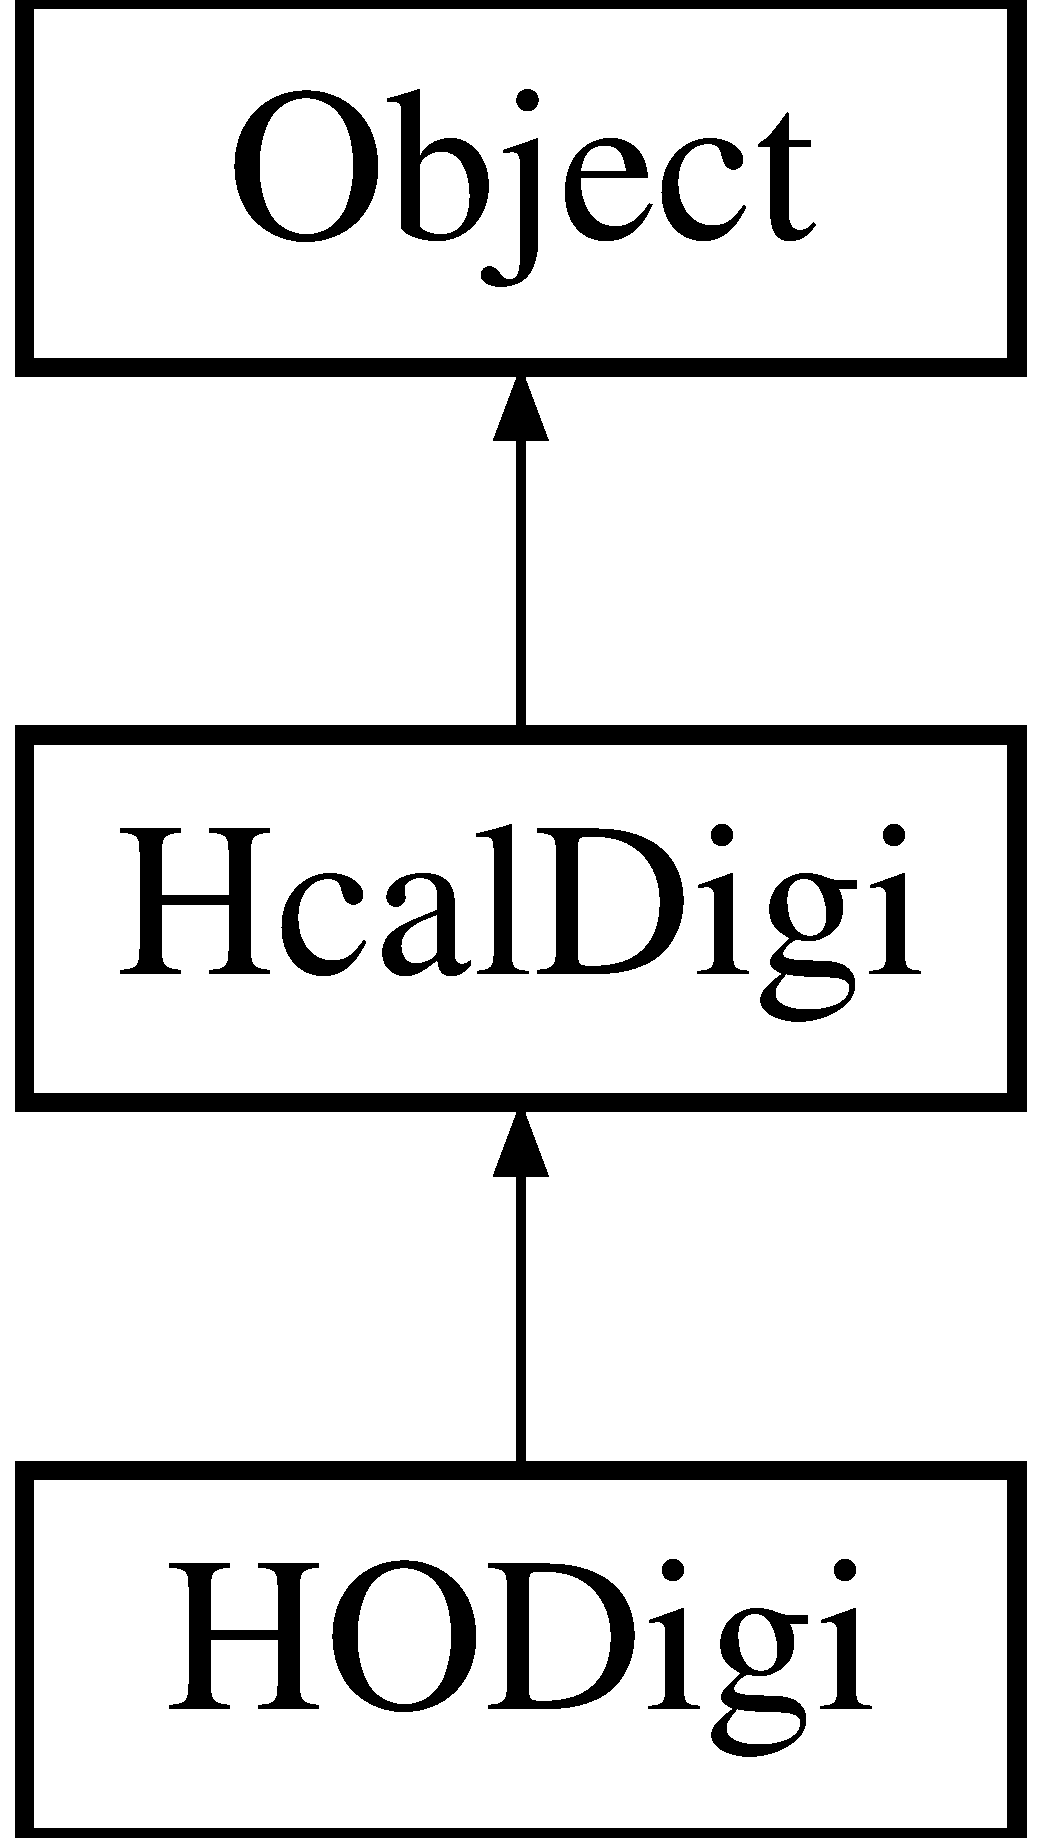
\includegraphics[height=3.000000cm]{class_h_o_digi}
\end{center}
\end{figure}
\subsection*{Public Member Functions}
\begin{DoxyCompactItemize}
\item 
\hyperlink{class_h_o_digi_adecf47054ae80a541c0bdac2a9f6207c}{H\+O\+Digi} ()
\item 
\hyperlink{class_h_o_digi_acf11a0e7224d491cc6461a056112bd2d}{H\+O\+Digi} (\hyperlink{class_collection}{Collection} \&c, unsigned short i, short j=0)
\item 
float \hyperlink{class_h_o_digi_a35507a821e8d2c511366d8ace55498e8}{energy} ()
\item 
float \hyperlink{class_h_o_digi_a838e14ae5420e4e8dc3666e1db6e88e4}{rec\+Hit\+Time} ()
\item 
int \hyperlink{class_h_o_digi_ade1d1693acbf00a041202f4077bc1b01}{ieta} ()
\item 
int \hyperlink{class_h_o_digi_a45538b8564e47fdfb4fa1f7b7b3638aa}{iphi} ()
\item 
int \hyperlink{class_h_o_digi_a9c7b71e89e76c571f222af1a994738f9}{depth} ()
\item 
int \hyperlink{class_h_o_digi_a4d7d71ce07087f9dcca70ef861ba1695}{size} ()
\item 
int \hyperlink{class_h_o_digi_a3f43041b8f83de05dd047a1174aef8c9}{presamples} ()
\item 
int \hyperlink{class_h_o_digi_ac26e1e5c799189bf1b75ab7d84693f04}{electronics\+Id} ()
\item 
int \hyperlink{class_h_o_digi_ad4db205e282e97906270b2277619431d}{raw\+Id} ()
\item 
float \hyperlink{class_h_o_digi_a56032f0b01bee6c79b9e22ff442b1226}{fc} (int i)
\item 
int \hyperlink{class_h_o_digi_a3e6b23ebca7eb32e5bc88176714e70c0}{adc} (int i)
\item 
int \hyperlink{class_h_o_digi_aa4ec10e56cab21dc97f357a613c6ac37}{dv} (int i)
\item 
int \hyperlink{class_h_o_digi_a7049efa78a9b03d356f0e25493c48de5}{er} (int i)
\item 
int \hyperlink{class_h_o_digi_a8058b129b0df409e8055506caae9b6e4}{capid} (int i)
\item 
float \hyperlink{class_h_o_digi_a02e8e6616c14c5f624d5d52a7fd10b7b}{gain} (int i)
\item 
int \hyperlink{class_h_o_digi_ac3a7701fee9cd02ee000ebab0e140a3d}{get\+Raw\+Index} ()
\item 
\hyperlink{class_h_o_sample}{H\+O\+Sample} \hyperlink{class_h_o_digi_a8b844b107f103dc2d7950f82734ad885}{operator\mbox{[}$\,$\mbox{]}} (int i)
\end{DoxyCompactItemize}
\subsection*{Public Attributes}
\begin{DoxyCompactItemize}
\item 
const int \hyperlink{class_h_o_digi_a72bdb21836d4e7dba0ad92f50cc652ab}{sum\+A\+D\+C} = \+\_\+sum\+A\+D\+C()
\end{DoxyCompactItemize}
\subsection*{Additional Inherited Members}


\subsection{Constructor \& Destructor Documentation}
\hypertarget{class_h_o_digi_adecf47054ae80a541c0bdac2a9f6207c}{}\index{H\+O\+Digi@{H\+O\+Digi}!H\+O\+Digi@{H\+O\+Digi}}
\index{H\+O\+Digi@{H\+O\+Digi}!H\+O\+Digi@{H\+O\+Digi}}
\subsubsection[{H\+O\+Digi()}]{\setlength{\rightskip}{0pt plus 5cm}H\+O\+Digi\+::\+H\+O\+Digi (
\begin{DoxyParamCaption}
{}
\end{DoxyParamCaption}
)}\label{class_h_o_digi_adecf47054ae80a541c0bdac2a9f6207c}
\hypertarget{class_h_o_digi_acf11a0e7224d491cc6461a056112bd2d}{}\index{H\+O\+Digi@{H\+O\+Digi}!H\+O\+Digi@{H\+O\+Digi}}
\index{H\+O\+Digi@{H\+O\+Digi}!H\+O\+Digi@{H\+O\+Digi}}
\subsubsection[{H\+O\+Digi(\+Collection \&c, unsigned short i, short j=0)}]{\setlength{\rightskip}{0pt plus 5cm}H\+O\+Digi\+::\+H\+O\+Digi (
\begin{DoxyParamCaption}
\item[{{\bf Collection} \&}]{c, }
\item[{unsigned short}]{i, }
\item[{short}]{j = {\ttfamily 0}}
\end{DoxyParamCaption}
)}\label{class_h_o_digi_acf11a0e7224d491cc6461a056112bd2d}


\subsection{Member Function Documentation}
\hypertarget{class_h_o_digi_a3e6b23ebca7eb32e5bc88176714e70c0}{}\index{H\+O\+Digi@{H\+O\+Digi}!adc@{adc}}
\index{adc@{adc}!H\+O\+Digi@{H\+O\+Digi}}
\subsubsection[{adc(int i)}]{\setlength{\rightskip}{0pt plus 5cm}int H\+O\+Digi\+::adc (
\begin{DoxyParamCaption}
\item[{int}]{i}
\end{DoxyParamCaption}
)\hspace{0.3cm}{\ttfamily [virtual]}}\label{class_h_o_digi_a3e6b23ebca7eb32e5bc88176714e70c0}


Implements \hyperlink{class_hcal_digi_a737b46ab9bc5439f32232ee6911ed516}{Hcal\+Digi}.

\hypertarget{class_h_o_digi_a8058b129b0df409e8055506caae9b6e4}{}\index{H\+O\+Digi@{H\+O\+Digi}!capid@{capid}}
\index{capid@{capid}!H\+O\+Digi@{H\+O\+Digi}}
\subsubsection[{capid(int i)}]{\setlength{\rightskip}{0pt plus 5cm}int H\+O\+Digi\+::capid (
\begin{DoxyParamCaption}
\item[{int}]{i}
\end{DoxyParamCaption}
)\hspace{0.3cm}{\ttfamily [virtual]}}\label{class_h_o_digi_a8058b129b0df409e8055506caae9b6e4}


Implements \hyperlink{class_hcal_digi_ad6e205312dda117af660b9391d502155}{Hcal\+Digi}.

\hypertarget{class_h_o_digi_a9c7b71e89e76c571f222af1a994738f9}{}\index{H\+O\+Digi@{H\+O\+Digi}!depth@{depth}}
\index{depth@{depth}!H\+O\+Digi@{H\+O\+Digi}}
\subsubsection[{depth()}]{\setlength{\rightskip}{0pt plus 5cm}int H\+O\+Digi\+::depth (
\begin{DoxyParamCaption}
{}
\end{DoxyParamCaption}
)\hspace{0.3cm}{\ttfamily [virtual]}}\label{class_h_o_digi_a9c7b71e89e76c571f222af1a994738f9}


Implements \hyperlink{class_hcal_digi_a916a582b044a64e041ba38e545349f7f}{Hcal\+Digi}.

\hypertarget{class_h_o_digi_aa4ec10e56cab21dc97f357a613c6ac37}{}\index{H\+O\+Digi@{H\+O\+Digi}!dv@{dv}}
\index{dv@{dv}!H\+O\+Digi@{H\+O\+Digi}}
\subsubsection[{dv(int i)}]{\setlength{\rightskip}{0pt plus 5cm}int H\+O\+Digi\+::dv (
\begin{DoxyParamCaption}
\item[{int}]{i}
\end{DoxyParamCaption}
)\hspace{0.3cm}{\ttfamily [virtual]}}\label{class_h_o_digi_aa4ec10e56cab21dc97f357a613c6ac37}


Implements \hyperlink{class_hcal_digi_aa758519b70ab24ac4bb7635052cfa174}{Hcal\+Digi}.

\hypertarget{class_h_o_digi_ac26e1e5c799189bf1b75ab7d84693f04}{}\index{H\+O\+Digi@{H\+O\+Digi}!electronics\+Id@{electronics\+Id}}
\index{electronics\+Id@{electronics\+Id}!H\+O\+Digi@{H\+O\+Digi}}
\subsubsection[{electronics\+Id()}]{\setlength{\rightskip}{0pt plus 5cm}int H\+O\+Digi\+::electronics\+Id (
\begin{DoxyParamCaption}
{}
\end{DoxyParamCaption}
)\hspace{0.3cm}{\ttfamily [virtual]}}\label{class_h_o_digi_ac26e1e5c799189bf1b75ab7d84693f04}


Implements \hyperlink{class_hcal_digi_afc95a09767a731b098cb2e22b89cc4e0}{Hcal\+Digi}.

\hypertarget{class_h_o_digi_a35507a821e8d2c511366d8ace55498e8}{}\index{H\+O\+Digi@{H\+O\+Digi}!energy@{energy}}
\index{energy@{energy}!H\+O\+Digi@{H\+O\+Digi}}
\subsubsection[{energy()}]{\setlength{\rightskip}{0pt plus 5cm}float H\+O\+Digi\+::energy (
\begin{DoxyParamCaption}
{}
\end{DoxyParamCaption}
)\hspace{0.3cm}{\ttfamily [virtual]}}\label{class_h_o_digi_a35507a821e8d2c511366d8ace55498e8}


Implements \hyperlink{class_hcal_digi_a665c0fa940132fafc6dce9fd75f18cea}{Hcal\+Digi}.

\hypertarget{class_h_o_digi_a7049efa78a9b03d356f0e25493c48de5}{}\index{H\+O\+Digi@{H\+O\+Digi}!er@{er}}
\index{er@{er}!H\+O\+Digi@{H\+O\+Digi}}
\subsubsection[{er(int i)}]{\setlength{\rightskip}{0pt plus 5cm}int H\+O\+Digi\+::er (
\begin{DoxyParamCaption}
\item[{int}]{i}
\end{DoxyParamCaption}
)\hspace{0.3cm}{\ttfamily [virtual]}}\label{class_h_o_digi_a7049efa78a9b03d356f0e25493c48de5}


Implements \hyperlink{class_hcal_digi_a04b02a86692bcdff2fb8fa8c50cc0c34}{Hcal\+Digi}.

\hypertarget{class_h_o_digi_a56032f0b01bee6c79b9e22ff442b1226}{}\index{H\+O\+Digi@{H\+O\+Digi}!fc@{fc}}
\index{fc@{fc}!H\+O\+Digi@{H\+O\+Digi}}
\subsubsection[{fc(int i)}]{\setlength{\rightskip}{0pt plus 5cm}float H\+O\+Digi\+::fc (
\begin{DoxyParamCaption}
\item[{int}]{i}
\end{DoxyParamCaption}
)\hspace{0.3cm}{\ttfamily [virtual]}}\label{class_h_o_digi_a56032f0b01bee6c79b9e22ff442b1226}


Implements \hyperlink{class_hcal_digi_a4a5e45ca390ee81fe384bf4a7d05f1e0}{Hcal\+Digi}.

\hypertarget{class_h_o_digi_a02e8e6616c14c5f624d5d52a7fd10b7b}{}\index{H\+O\+Digi@{H\+O\+Digi}!gain@{gain}}
\index{gain@{gain}!H\+O\+Digi@{H\+O\+Digi}}
\subsubsection[{gain(int i)}]{\setlength{\rightskip}{0pt plus 5cm}float H\+O\+Digi\+::gain (
\begin{DoxyParamCaption}
\item[{int}]{i}
\end{DoxyParamCaption}
)}\label{class_h_o_digi_a02e8e6616c14c5f624d5d52a7fd10b7b}
\hypertarget{class_h_o_digi_ac3a7701fee9cd02ee000ebab0e140a3d}{}\index{H\+O\+Digi@{H\+O\+Digi}!get\+Raw\+Index@{get\+Raw\+Index}}
\index{get\+Raw\+Index@{get\+Raw\+Index}!H\+O\+Digi@{H\+O\+Digi}}
\subsubsection[{get\+Raw\+Index()}]{\setlength{\rightskip}{0pt plus 5cm}int H\+O\+Digi\+::get\+Raw\+Index (
\begin{DoxyParamCaption}
{}
\end{DoxyParamCaption}
)\hspace{0.3cm}{\ttfamily [inline]}}\label{class_h_o_digi_ac3a7701fee9cd02ee000ebab0e140a3d}
\hypertarget{class_h_o_digi_ade1d1693acbf00a041202f4077bc1b01}{}\index{H\+O\+Digi@{H\+O\+Digi}!ieta@{ieta}}
\index{ieta@{ieta}!H\+O\+Digi@{H\+O\+Digi}}
\subsubsection[{ieta()}]{\setlength{\rightskip}{0pt plus 5cm}int H\+O\+Digi\+::ieta (
\begin{DoxyParamCaption}
{}
\end{DoxyParamCaption}
)\hspace{0.3cm}{\ttfamily [virtual]}}\label{class_h_o_digi_ade1d1693acbf00a041202f4077bc1b01}


Implements \hyperlink{class_hcal_digi_a65fc605c5c3bca7f78d961400d145c94}{Hcal\+Digi}.

\hypertarget{class_h_o_digi_a45538b8564e47fdfb4fa1f7b7b3638aa}{}\index{H\+O\+Digi@{H\+O\+Digi}!iphi@{iphi}}
\index{iphi@{iphi}!H\+O\+Digi@{H\+O\+Digi}}
\subsubsection[{iphi()}]{\setlength{\rightskip}{0pt plus 5cm}int H\+O\+Digi\+::iphi (
\begin{DoxyParamCaption}
{}
\end{DoxyParamCaption}
)\hspace{0.3cm}{\ttfamily [virtual]}}\label{class_h_o_digi_a45538b8564e47fdfb4fa1f7b7b3638aa}


Implements \hyperlink{class_hcal_digi_a979dec4585c9d07a7dc4060dfb97f089}{Hcal\+Digi}.

\hypertarget{class_h_o_digi_a8b844b107f103dc2d7950f82734ad885}{}\index{H\+O\+Digi@{H\+O\+Digi}!operator\mbox{[}$\,$\mbox{]}@{operator[]}}
\index{operator\mbox{[}$\,$\mbox{]}@{operator[]}!H\+O\+Digi@{H\+O\+Digi}}
\subsubsection[{operator[](int i)}]{\setlength{\rightskip}{0pt plus 5cm}{\bf H\+O\+Sample} H\+O\+Digi\+::operator\mbox{[}$\,$\mbox{]} (
\begin{DoxyParamCaption}
\item[{int}]{i}
\end{DoxyParamCaption}
)\hspace{0.3cm}{\ttfamily [inline]}}\label{class_h_o_digi_a8b844b107f103dc2d7950f82734ad885}
\hypertarget{class_h_o_digi_a3f43041b8f83de05dd047a1174aef8c9}{}\index{H\+O\+Digi@{H\+O\+Digi}!presamples@{presamples}}
\index{presamples@{presamples}!H\+O\+Digi@{H\+O\+Digi}}
\subsubsection[{presamples()}]{\setlength{\rightskip}{0pt plus 5cm}int H\+O\+Digi\+::presamples (
\begin{DoxyParamCaption}
{}
\end{DoxyParamCaption}
)\hspace{0.3cm}{\ttfamily [virtual]}}\label{class_h_o_digi_a3f43041b8f83de05dd047a1174aef8c9}


Implements \hyperlink{class_hcal_digi_aad0fc232379d8bdd40d6be32b3c980c4}{Hcal\+Digi}.

\hypertarget{class_h_o_digi_ad4db205e282e97906270b2277619431d}{}\index{H\+O\+Digi@{H\+O\+Digi}!raw\+Id@{raw\+Id}}
\index{raw\+Id@{raw\+Id}!H\+O\+Digi@{H\+O\+Digi}}
\subsubsection[{raw\+Id()}]{\setlength{\rightskip}{0pt plus 5cm}int H\+O\+Digi\+::raw\+Id (
\begin{DoxyParamCaption}
{}
\end{DoxyParamCaption}
)\hspace{0.3cm}{\ttfamily [virtual]}}\label{class_h_o_digi_ad4db205e282e97906270b2277619431d}


Implements \hyperlink{class_hcal_digi_aba55732d16499ad510091c769807f8e1}{Hcal\+Digi}.

\hypertarget{class_h_o_digi_a838e14ae5420e4e8dc3666e1db6e88e4}{}\index{H\+O\+Digi@{H\+O\+Digi}!rec\+Hit\+Time@{rec\+Hit\+Time}}
\index{rec\+Hit\+Time@{rec\+Hit\+Time}!H\+O\+Digi@{H\+O\+Digi}}
\subsubsection[{rec\+Hit\+Time()}]{\setlength{\rightskip}{0pt plus 5cm}float H\+O\+Digi\+::rec\+Hit\+Time (
\begin{DoxyParamCaption}
{}
\end{DoxyParamCaption}
)\hspace{0.3cm}{\ttfamily [virtual]}}\label{class_h_o_digi_a838e14ae5420e4e8dc3666e1db6e88e4}


Implements \hyperlink{class_hcal_digi_a3936cda623fc7535ed35d8d1c6abb350}{Hcal\+Digi}.

\hypertarget{class_h_o_digi_a4d7d71ce07087f9dcca70ef861ba1695}{}\index{H\+O\+Digi@{H\+O\+Digi}!size@{size}}
\index{size@{size}!H\+O\+Digi@{H\+O\+Digi}}
\subsubsection[{size()}]{\setlength{\rightskip}{0pt plus 5cm}int H\+O\+Digi\+::size (
\begin{DoxyParamCaption}
{}
\end{DoxyParamCaption}
)\hspace{0.3cm}{\ttfamily [virtual]}}\label{class_h_o_digi_a4d7d71ce07087f9dcca70ef861ba1695}


Implements \hyperlink{class_hcal_digi_a054f6f17539c8042d2900144d06eb4fc}{Hcal\+Digi}.



\subsection{Member Data Documentation}
\hypertarget{class_h_o_digi_a72bdb21836d4e7dba0ad92f50cc652ab}{}\index{H\+O\+Digi@{H\+O\+Digi}!sum\+A\+D\+C@{sum\+A\+D\+C}}
\index{sum\+A\+D\+C@{sum\+A\+D\+C}!H\+O\+Digi@{H\+O\+Digi}}
\subsubsection[{sum\+A\+D\+C}]{\setlength{\rightskip}{0pt plus 5cm}const int H\+O\+Digi\+::sum\+A\+D\+C = \+\_\+sum\+A\+D\+C()}\label{class_h_o_digi_a72bdb21836d4e7dba0ad92f50cc652ab}


The documentation for this class was generated from the following files\+:\begin{DoxyCompactItemize}
\item 
interface/\hyperlink{_h_o_digi_8h}{H\+O\+Digi.\+h}\item 
src/\hyperlink{_h_o_digi_8cc}{H\+O\+Digi.\+cc}\end{DoxyCompactItemize}

\hypertarget{class_h_o_sample}{}\section{H\+O\+Sample Class Reference}
\label{class_h_o_sample}\index{H\+O\+Sample@{H\+O\+Sample}}


{\ttfamily \#include $<$H\+O\+Sample.\+h$>$}

Inheritance diagram for H\+O\+Sample\+:\begin{figure}[H]
\begin{center}
\leavevmode
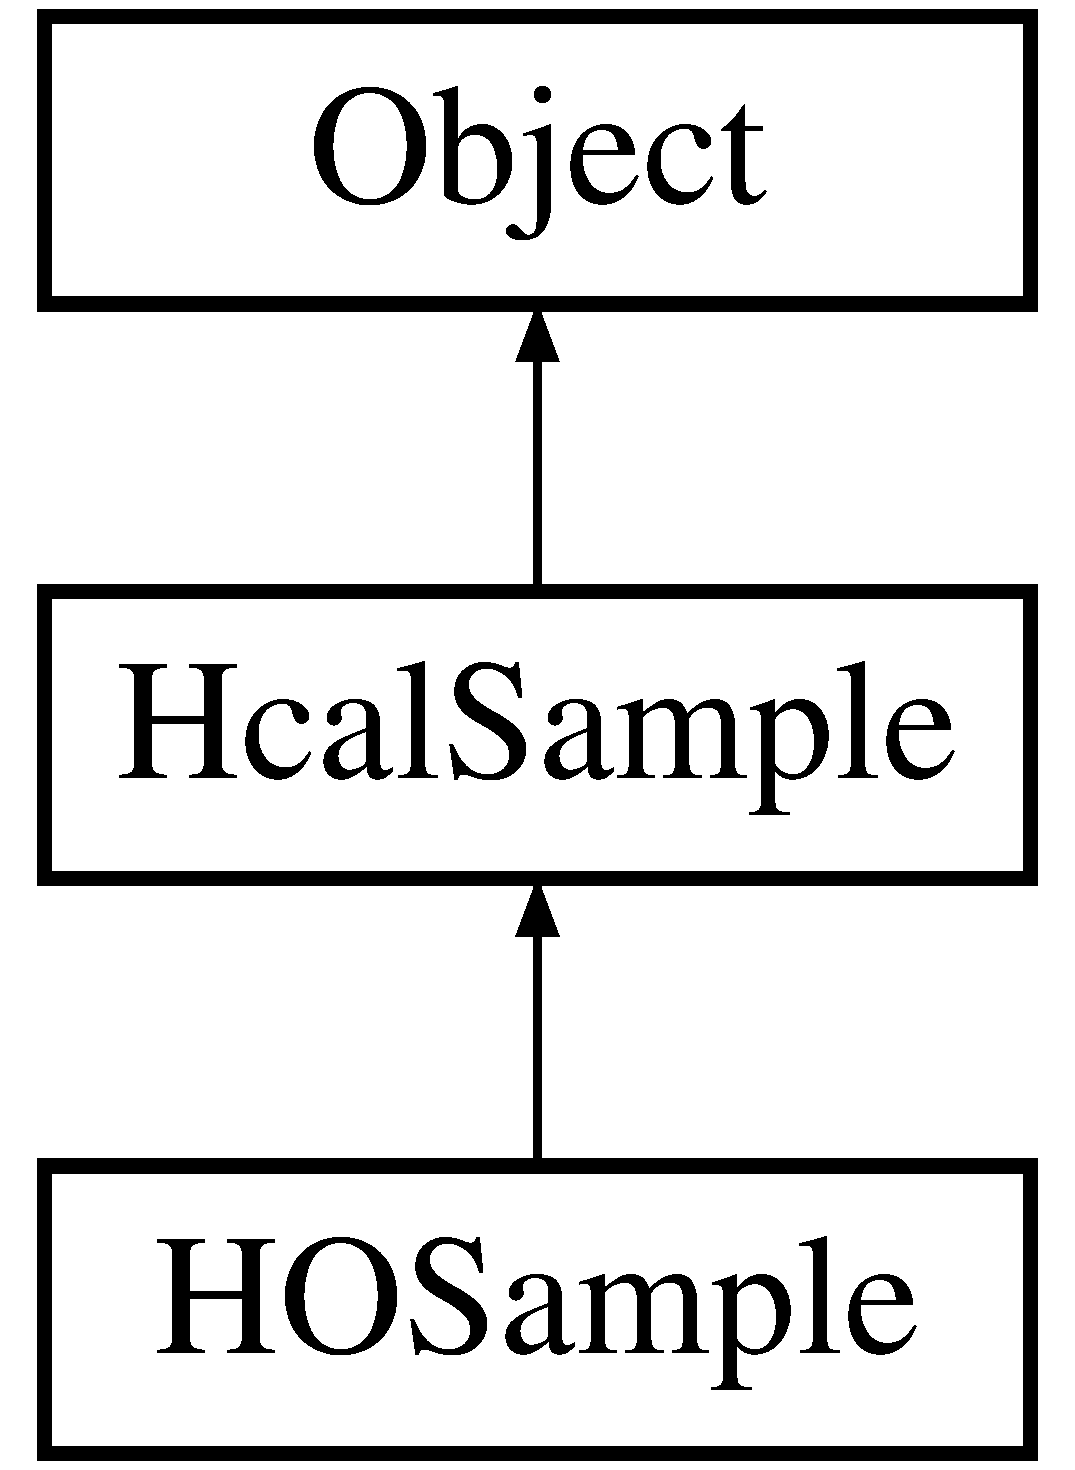
\includegraphics[height=3.000000cm]{class_h_o_sample}
\end{center}
\end{figure}
\subsection*{Public Member Functions}
\begin{DoxyCompactItemize}
\item 
\hyperlink{class_h_o_sample_aebc830cc129a8b88b7fb36d2d05a5bb0}{H\+O\+Sample} ()
\item 
\hyperlink{class_h_o_sample_a2ae3c7775da1bc012675cce8c16a606c}{H\+O\+Sample} (\hyperlink{class_collection}{Collection} \&c, unsigned short i, short j)
\item 
float \hyperlink{class_h_o_sample_a7517db4397842a88372e74a0e769d270}{all\+F\+C} ()
\item 
float \hyperlink{class_h_o_sample_a94767275b31209a74a9d8169ee88276d}{energy} ()
\item 
float \hyperlink{class_h_o_sample_adc4aeb23e36cea824ce18dbdf57ffbc2}{gain} ()
\item 
float \hyperlink{class_h_o_sample_aca3d42b2fd9431719f849542ebfdf2a9}{fc} ()
\item 
float \hyperlink{class_h_o_sample_a403853f4477960ae93988c5629a28c0c}{nom\+F\+C} ()
\item 
float \hyperlink{class_h_o_sample_afccd544265c85885bce27d960aa81741}{ped\+F\+C} ()
\item 
float \hyperlink{class_h_o_sample_aed754b102ffe962139bb216df35a308f}{rc\+Gain} ()
\item 
int \hyperlink{class_h_o_sample_adb4388064b1512918b527fa0ded051e1}{adc} ()
\item 
int \hyperlink{class_h_o_sample_aae92efbb6b23b511c923a84723811dfe}{capid} ()
\item 
int \hyperlink{class_h_o_sample_a3fcb610100099d07f030249da9160aaa}{dv} ()
\item 
int \hyperlink{class_h_o_sample_ae63dde72730e4ab5a08e0b4b5a0ba19e}{er} ()
\item 
int \hyperlink{class_h_o_sample_a59d656a291cb5e7242c27fed2346a3a7}{fiber} ()
\item 
int \hyperlink{class_h_o_sample_a136f3641f4e0cafd6270fe4006acd499}{fiber\+Chan} ()
\item 
int \hyperlink{class_h_o_sample_ad4e252cf8313d9072f7162df3ac4c5af}{raw} ()
\item 
int \hyperlink{class_h_o_sample_afbdcd06c316d490a400af426ae08bbaf}{get\+Raw\+Index} ()
\item 
int \hyperlink{class_h_o_sample_aab7462a4521717cb5f0a88aeece239f7}{get\+Time\+Slice} ()
\end{DoxyCompactItemize}
\subsection*{Additional Inherited Members}


\subsection{Constructor \& Destructor Documentation}
\hypertarget{class_h_o_sample_aebc830cc129a8b88b7fb36d2d05a5bb0}{}\index{H\+O\+Sample@{H\+O\+Sample}!H\+O\+Sample@{H\+O\+Sample}}
\index{H\+O\+Sample@{H\+O\+Sample}!H\+O\+Sample@{H\+O\+Sample}}
\subsubsection[{H\+O\+Sample()}]{\setlength{\rightskip}{0pt plus 5cm}H\+O\+Sample\+::\+H\+O\+Sample (
\begin{DoxyParamCaption}
{}
\end{DoxyParamCaption}
)}\label{class_h_o_sample_aebc830cc129a8b88b7fb36d2d05a5bb0}
\hypertarget{class_h_o_sample_a2ae3c7775da1bc012675cce8c16a606c}{}\index{H\+O\+Sample@{H\+O\+Sample}!H\+O\+Sample@{H\+O\+Sample}}
\index{H\+O\+Sample@{H\+O\+Sample}!H\+O\+Sample@{H\+O\+Sample}}
\subsubsection[{H\+O\+Sample(\+Collection \&c, unsigned short i, short j)}]{\setlength{\rightskip}{0pt plus 5cm}H\+O\+Sample\+::\+H\+O\+Sample (
\begin{DoxyParamCaption}
\item[{{\bf Collection} \&}]{c, }
\item[{unsigned short}]{i, }
\item[{short}]{j}
\end{DoxyParamCaption}
)}\label{class_h_o_sample_a2ae3c7775da1bc012675cce8c16a606c}


\subsection{Member Function Documentation}
\hypertarget{class_h_o_sample_adb4388064b1512918b527fa0ded051e1}{}\index{H\+O\+Sample@{H\+O\+Sample}!adc@{adc}}
\index{adc@{adc}!H\+O\+Sample@{H\+O\+Sample}}
\subsubsection[{adc()}]{\setlength{\rightskip}{0pt plus 5cm}int H\+O\+Sample\+::adc (
\begin{DoxyParamCaption}
{}
\end{DoxyParamCaption}
)\hspace{0.3cm}{\ttfamily [virtual]}}\label{class_h_o_sample_adb4388064b1512918b527fa0ded051e1}


Implements \hyperlink{class_hcal_sample_a3801777ac080ca0e512c226e4cfd5682}{Hcal\+Sample}.

\hypertarget{class_h_o_sample_a7517db4397842a88372e74a0e769d270}{}\index{H\+O\+Sample@{H\+O\+Sample}!all\+F\+C@{all\+F\+C}}
\index{all\+F\+C@{all\+F\+C}!H\+O\+Sample@{H\+O\+Sample}}
\subsubsection[{all\+F\+C()}]{\setlength{\rightskip}{0pt plus 5cm}float H\+O\+Sample\+::all\+F\+C (
\begin{DoxyParamCaption}
{}
\end{DoxyParamCaption}
)\hspace{0.3cm}{\ttfamily [virtual]}}\label{class_h_o_sample_a7517db4397842a88372e74a0e769d270}


Implements \hyperlink{class_hcal_sample_af837bd894eb8eae865023a526940ee15}{Hcal\+Sample}.

\hypertarget{class_h_o_sample_aae92efbb6b23b511c923a84723811dfe}{}\index{H\+O\+Sample@{H\+O\+Sample}!capid@{capid}}
\index{capid@{capid}!H\+O\+Sample@{H\+O\+Sample}}
\subsubsection[{capid()}]{\setlength{\rightskip}{0pt plus 5cm}int H\+O\+Sample\+::capid (
\begin{DoxyParamCaption}
{}
\end{DoxyParamCaption}
)\hspace{0.3cm}{\ttfamily [virtual]}}\label{class_h_o_sample_aae92efbb6b23b511c923a84723811dfe}


Implements \hyperlink{class_hcal_sample_a51a82042ba140a68f9659140c48d83bc}{Hcal\+Sample}.

\hypertarget{class_h_o_sample_a3fcb610100099d07f030249da9160aaa}{}\index{H\+O\+Sample@{H\+O\+Sample}!dv@{dv}}
\index{dv@{dv}!H\+O\+Sample@{H\+O\+Sample}}
\subsubsection[{dv()}]{\setlength{\rightskip}{0pt plus 5cm}int H\+O\+Sample\+::dv (
\begin{DoxyParamCaption}
{}
\end{DoxyParamCaption}
)\hspace{0.3cm}{\ttfamily [virtual]}}\label{class_h_o_sample_a3fcb610100099d07f030249da9160aaa}


Implements \hyperlink{class_hcal_sample_a13c0e851a42d3122c7bba32d81e31d19}{Hcal\+Sample}.

\hypertarget{class_h_o_sample_a94767275b31209a74a9d8169ee88276d}{}\index{H\+O\+Sample@{H\+O\+Sample}!energy@{energy}}
\index{energy@{energy}!H\+O\+Sample@{H\+O\+Sample}}
\subsubsection[{energy()}]{\setlength{\rightskip}{0pt plus 5cm}float H\+O\+Sample\+::energy (
\begin{DoxyParamCaption}
{}
\end{DoxyParamCaption}
)\hspace{0.3cm}{\ttfamily [virtual]}}\label{class_h_o_sample_a94767275b31209a74a9d8169ee88276d}


Implements \hyperlink{class_hcal_sample_a603c4e95d1d49db37dd00f34275fb8f3}{Hcal\+Sample}.

\hypertarget{class_h_o_sample_ae63dde72730e4ab5a08e0b4b5a0ba19e}{}\index{H\+O\+Sample@{H\+O\+Sample}!er@{er}}
\index{er@{er}!H\+O\+Sample@{H\+O\+Sample}}
\subsubsection[{er()}]{\setlength{\rightskip}{0pt plus 5cm}int H\+O\+Sample\+::er (
\begin{DoxyParamCaption}
{}
\end{DoxyParamCaption}
)\hspace{0.3cm}{\ttfamily [virtual]}}\label{class_h_o_sample_ae63dde72730e4ab5a08e0b4b5a0ba19e}


Implements \hyperlink{class_hcal_sample_af1805d239ccbc17a6c307d66522da618}{Hcal\+Sample}.

\hypertarget{class_h_o_sample_aca3d42b2fd9431719f849542ebfdf2a9}{}\index{H\+O\+Sample@{H\+O\+Sample}!fc@{fc}}
\index{fc@{fc}!H\+O\+Sample@{H\+O\+Sample}}
\subsubsection[{fc()}]{\setlength{\rightskip}{0pt plus 5cm}float H\+O\+Sample\+::fc (
\begin{DoxyParamCaption}
{}
\end{DoxyParamCaption}
)\hspace{0.3cm}{\ttfamily [virtual]}}\label{class_h_o_sample_aca3d42b2fd9431719f849542ebfdf2a9}


Implements \hyperlink{class_hcal_sample_aed932c9f932eabed9f9bc6b1a54c20dd}{Hcal\+Sample}.

\hypertarget{class_h_o_sample_a59d656a291cb5e7242c27fed2346a3a7}{}\index{H\+O\+Sample@{H\+O\+Sample}!fiber@{fiber}}
\index{fiber@{fiber}!H\+O\+Sample@{H\+O\+Sample}}
\subsubsection[{fiber()}]{\setlength{\rightskip}{0pt plus 5cm}int H\+O\+Sample\+::fiber (
\begin{DoxyParamCaption}
{}
\end{DoxyParamCaption}
)\hspace{0.3cm}{\ttfamily [virtual]}}\label{class_h_o_sample_a59d656a291cb5e7242c27fed2346a3a7}


Implements \hyperlink{class_hcal_sample_a5ae9a4d213b69f5ee382c7a6b31eb446}{Hcal\+Sample}.

\hypertarget{class_h_o_sample_a136f3641f4e0cafd6270fe4006acd499}{}\index{H\+O\+Sample@{H\+O\+Sample}!fiber\+Chan@{fiber\+Chan}}
\index{fiber\+Chan@{fiber\+Chan}!H\+O\+Sample@{H\+O\+Sample}}
\subsubsection[{fiber\+Chan()}]{\setlength{\rightskip}{0pt plus 5cm}int H\+O\+Sample\+::fiber\+Chan (
\begin{DoxyParamCaption}
{}
\end{DoxyParamCaption}
)\hspace{0.3cm}{\ttfamily [virtual]}}\label{class_h_o_sample_a136f3641f4e0cafd6270fe4006acd499}


Implements \hyperlink{class_hcal_sample_acdd36acaedfe4e1a6114e6c56d1ed996}{Hcal\+Sample}.

\hypertarget{class_h_o_sample_adc4aeb23e36cea824ce18dbdf57ffbc2}{}\index{H\+O\+Sample@{H\+O\+Sample}!gain@{gain}}
\index{gain@{gain}!H\+O\+Sample@{H\+O\+Sample}}
\subsubsection[{gain()}]{\setlength{\rightskip}{0pt plus 5cm}float H\+O\+Sample\+::gain (
\begin{DoxyParamCaption}
{}
\end{DoxyParamCaption}
)\hspace{0.3cm}{\ttfamily [virtual]}}\label{class_h_o_sample_adc4aeb23e36cea824ce18dbdf57ffbc2}


Implements \hyperlink{class_hcal_sample_aefc3dd058b3b178917583ca6abbf4f01}{Hcal\+Sample}.

\hypertarget{class_h_o_sample_afbdcd06c316d490a400af426ae08bbaf}{}\index{H\+O\+Sample@{H\+O\+Sample}!get\+Raw\+Index@{get\+Raw\+Index}}
\index{get\+Raw\+Index@{get\+Raw\+Index}!H\+O\+Sample@{H\+O\+Sample}}
\subsubsection[{get\+Raw\+Index()}]{\setlength{\rightskip}{0pt plus 5cm}int H\+O\+Sample\+::get\+Raw\+Index (
\begin{DoxyParamCaption}
{}
\end{DoxyParamCaption}
)\hspace{0.3cm}{\ttfamily [inline]}}\label{class_h_o_sample_afbdcd06c316d490a400af426ae08bbaf}
\hypertarget{class_h_o_sample_aab7462a4521717cb5f0a88aeece239f7}{}\index{H\+O\+Sample@{H\+O\+Sample}!get\+Time\+Slice@{get\+Time\+Slice}}
\index{get\+Time\+Slice@{get\+Time\+Slice}!H\+O\+Sample@{H\+O\+Sample}}
\subsubsection[{get\+Time\+Slice()}]{\setlength{\rightskip}{0pt plus 5cm}int H\+O\+Sample\+::get\+Time\+Slice (
\begin{DoxyParamCaption}
{}
\end{DoxyParamCaption}
)\hspace{0.3cm}{\ttfamily [inline]}}\label{class_h_o_sample_aab7462a4521717cb5f0a88aeece239f7}
\hypertarget{class_h_o_sample_a403853f4477960ae93988c5629a28c0c}{}\index{H\+O\+Sample@{H\+O\+Sample}!nom\+F\+C@{nom\+F\+C}}
\index{nom\+F\+C@{nom\+F\+C}!H\+O\+Sample@{H\+O\+Sample}}
\subsubsection[{nom\+F\+C()}]{\setlength{\rightskip}{0pt plus 5cm}float H\+O\+Sample\+::nom\+F\+C (
\begin{DoxyParamCaption}
{}
\end{DoxyParamCaption}
)\hspace{0.3cm}{\ttfamily [virtual]}}\label{class_h_o_sample_a403853f4477960ae93988c5629a28c0c}


Implements \hyperlink{class_hcal_sample_a9f47a5b867c94c97c3d553e244e7dc87}{Hcal\+Sample}.

\hypertarget{class_h_o_sample_afccd544265c85885bce27d960aa81741}{}\index{H\+O\+Sample@{H\+O\+Sample}!ped\+F\+C@{ped\+F\+C}}
\index{ped\+F\+C@{ped\+F\+C}!H\+O\+Sample@{H\+O\+Sample}}
\subsubsection[{ped\+F\+C()}]{\setlength{\rightskip}{0pt plus 5cm}float H\+O\+Sample\+::ped\+F\+C (
\begin{DoxyParamCaption}
{}
\end{DoxyParamCaption}
)\hspace{0.3cm}{\ttfamily [virtual]}}\label{class_h_o_sample_afccd544265c85885bce27d960aa81741}


Implements \hyperlink{class_hcal_sample_a471f7ef87944ac870ea884a0cc957744}{Hcal\+Sample}.

\hypertarget{class_h_o_sample_ad4e252cf8313d9072f7162df3ac4c5af}{}\index{H\+O\+Sample@{H\+O\+Sample}!raw@{raw}}
\index{raw@{raw}!H\+O\+Sample@{H\+O\+Sample}}
\subsubsection[{raw()}]{\setlength{\rightskip}{0pt plus 5cm}int H\+O\+Sample\+::raw (
\begin{DoxyParamCaption}
{}
\end{DoxyParamCaption}
)\hspace{0.3cm}{\ttfamily [virtual]}}\label{class_h_o_sample_ad4e252cf8313d9072f7162df3ac4c5af}


Implements \hyperlink{class_hcal_sample_a328a0f8f80a0aae47a92500297635bd6}{Hcal\+Sample}.

\hypertarget{class_h_o_sample_aed754b102ffe962139bb216df35a308f}{}\index{H\+O\+Sample@{H\+O\+Sample}!rc\+Gain@{rc\+Gain}}
\index{rc\+Gain@{rc\+Gain}!H\+O\+Sample@{H\+O\+Sample}}
\subsubsection[{rc\+Gain()}]{\setlength{\rightskip}{0pt plus 5cm}float H\+O\+Sample\+::rc\+Gain (
\begin{DoxyParamCaption}
{}
\end{DoxyParamCaption}
)\hspace{0.3cm}{\ttfamily [virtual]}}\label{class_h_o_sample_aed754b102ffe962139bb216df35a308f}


Implements \hyperlink{class_hcal_sample_a6fd32da2d5ea80154251de366f98c49c}{Hcal\+Sample}.



The documentation for this class was generated from the following files\+:\begin{DoxyCompactItemize}
\item 
interface/\hyperlink{_h_o_sample_8h}{H\+O\+Sample.\+h}\item 
src/\hyperlink{_h_o_sample_8cc}{H\+O\+Sample.\+cc}\end{DoxyCompactItemize}

\hypertarget{class_object}{}\section{Object Class Reference}
\label{class_object}\index{Object@{Object}}


{\ttfamily \#include $<$Object.\+h$>$}

Inheritance diagram for Object\+:\begin{figure}[H]
\begin{center}
\leavevmode
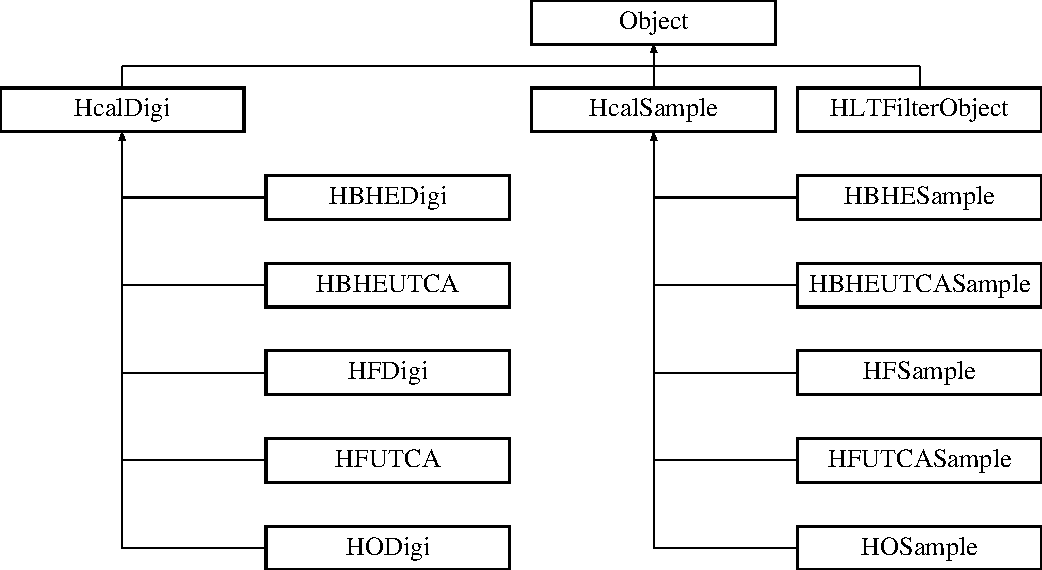
\includegraphics[height=7.000000cm]{class_object}
\end{center}
\end{figure}
\subsection*{Public Member Functions}
\begin{DoxyCompactItemize}
\item 
\hyperlink{class_object_a40860402e64d8008fb42329df7097cdb}{Object} ()
\item 
\hyperlink{class_object_af3b5cd7a9a24ddde484344200cf83281}{Object} (const \hyperlink{class_object}{Object} \&)
\item 
\hyperlink{class_object_a4cab32d7c391abd44858b62a291a63af}{Object} (\hyperlink{class_collection}{Collection} \&collection, short raw\+\_\+index)
\item 
\hyperlink{class_object_ab53a90984c2f5ce5c56844729e2a9423}{Object} (\hyperlink{class_collection}{Collection} \&collection, short raw\+\_\+index, const char $\ast$name)
\item 
\hyperlink{class_object_a0e5c30a0657fe9466ac0929bc9460a01}{Object} (\hyperlink{class_collection}{Collection} \&collection, short raw\+\_\+index, short hlt\+\_\+filter\+\_\+index)
\item 
\hyperlink{class_object_ae50594e498a111e905387e0313c801f4}{Object} (\hyperlink{class_collection}{Collection} \&collection, short raw\+\_\+index, short hlt\+\_\+filter\+\_\+index, const char $\ast$name)
\item 
\hyperlink{class_object_ae8f5483f459e46687bd01e6f9977afd3}{$\sim$\+Object} ()
\item 
const char $\ast$ \hyperlink{class_object_a57442be9a5695f873a22787a107ec01b}{Name} () const 
\item 
virtual short \hyperlink{class_object_a6c5f158e839949047e4cb14489aae4ca}{Get\+Raw\+Index} ()
\item 
virtual double \& \hyperlink{class_object_ac280f2330a4bd359404841431bd46f2e}{Pt} ()=0
\item 
virtual double \& \hyperlink{class_object_ab8fa3bfbd16c2b6c420ec113fbc2a0e4}{Phi} ()=0
\item 
virtual double \& \hyperlink{class_object_a3760d2b4b0723118234370675654d46a}{Eta} ()=0
\item 
virtual double \hyperlink{class_object_abf0816d94dbf5512710b160f54779c98}{Energy\+Res\+Scale\+Factor} ()
\item 
virtual double \hyperlink{class_object_ae1afc1bad2f56db046023a9776eba93f}{Energy\+Scale\+Factor} ()
\item 
virtual double \hyperlink{class_object_a492c12bfcde7d1a7c36722cfc7977e92}{Energy\+Res\+Scale\+Error} ()
\item 
virtual bool \hyperlink{class_object_ae28bc9879447dad23f10ebd1971e81f5}{Pass\+User\+I\+D} (\hyperlink{_i_d_types_8h_a094c367727273b4da2b960ca3b3edc06}{I\+D} id, bool verbose)=0
\item 
double \hyperlink{class_object_a5f825f0cdc0f45ec3efbea0bd1bc4c6a}{Delta\+R} (\hyperlink{class_object}{Object} $\ast$other\+\_\+object)
\item 
double \hyperlink{class_object_aaa50373e27e16bf086e0a2a24ae8a37b}{Delta\+Phi} (\hyperlink{class_object}{Object} $\ast$other\+\_\+object)
\item 
double \hyperlink{class_object_aaa45210cbaa92c8bb0e010c11a83c58c}{Phi\+\_\+mpi\+\_\+pi} (double x)
\item 
bool \hyperlink{class_object_a6b0f2caacff9cac58cae48f859546715}{Is\+Gen\+E\+B\+Fiducial} ()
\item 
bool \hyperlink{class_object_ac0980938e66610abc54ddbd4548410cf}{Is\+Gen\+E\+E\+Fiducial} ()
\item 
bool \hyperlink{class_object_ac29c9d8a48d0369ac06e921b578c0478}{Is\+Gen\+Electron\+Fiducial} ()
\item 
bool \hyperlink{class_object_a4f86f3820ed2571046d520047d2db7ae}{Is\+Muon\+Fiducial} ()
\item 
bool \hyperlink{class_object_afcf15ef137aabe615be23f6db585a779}{Is\+N\+U\+L\+L} ()
\item 
{\footnotesize template$<$class Another\+Object $>$ }\\bool \hyperlink{class_object_a1a01cc0958c3b491c26c2a066314481c}{Match\+By\+D\+R} (\hyperlink{_collection_8h_a64ea9217513944abee0afcb2ee82d787}{Collection\+Ptr} c, Another\+Object \&best\+\_\+match, double max\+\_\+dr)
\end{DoxyCompactItemize}
\subsection*{Protected Attributes}
\begin{DoxyCompactItemize}
\item 
const char $\ast$ \hyperlink{class_object_a90fd7f91e8f0f3eea7bc1eeed71ec3d6}{m\+\_\+name}
\item 
\hyperlink{class_collection}{Collection} $\ast$ \hyperlink{class_object_af66cc1db553fa91b451c7855a8d09ec0}{m\+\_\+collection}
\item 
short \hyperlink{class_object_a75e13245ae926f83a29ce9b25b8e4aa5}{m\+\_\+raw\+\_\+index}
\item 
short \hyperlink{class_object_ac1f71ac949f9d66cdeabca5dc7385a03}{m\+\_\+hlt\+\_\+filter\+\_\+index}
\end{DoxyCompactItemize}


\subsection{Constructor \& Destructor Documentation}
\hypertarget{class_object_a40860402e64d8008fb42329df7097cdb}{}\index{Object@{Object}!Object@{Object}}
\index{Object@{Object}!Object@{Object}}
\subsubsection[{Object()}]{\setlength{\rightskip}{0pt plus 5cm}Object\+::\+Object (
\begin{DoxyParamCaption}
{}
\end{DoxyParamCaption}
)}\label{class_object_a40860402e64d8008fb42329df7097cdb}
\hypertarget{class_object_af3b5cd7a9a24ddde484344200cf83281}{}\index{Object@{Object}!Object@{Object}}
\index{Object@{Object}!Object@{Object}}
\subsubsection[{Object(const Object \&)}]{\setlength{\rightskip}{0pt plus 5cm}Object\+::\+Object (
\begin{DoxyParamCaption}
\item[{const {\bf Object} \&}]{o}
\end{DoxyParamCaption}
)}\label{class_object_af3b5cd7a9a24ddde484344200cf83281}
\hypertarget{class_object_a4cab32d7c391abd44858b62a291a63af}{}\index{Object@{Object}!Object@{Object}}
\index{Object@{Object}!Object@{Object}}
\subsubsection[{Object(\+Collection \&collection, short raw\+\_\+index)}]{\setlength{\rightskip}{0pt plus 5cm}Object\+::\+Object (
\begin{DoxyParamCaption}
\item[{{\bf Collection} \&}]{collection, }
\item[{short}]{raw\+\_\+index}
\end{DoxyParamCaption}
)}\label{class_object_a4cab32d7c391abd44858b62a291a63af}
\hypertarget{class_object_ab53a90984c2f5ce5c56844729e2a9423}{}\index{Object@{Object}!Object@{Object}}
\index{Object@{Object}!Object@{Object}}
\subsubsection[{Object(\+Collection \&collection, short raw\+\_\+index, const char $\ast$name)}]{\setlength{\rightskip}{0pt plus 5cm}Object\+::\+Object (
\begin{DoxyParamCaption}
\item[{{\bf Collection} \&}]{collection, }
\item[{short}]{raw\+\_\+index, }
\item[{const char $\ast$}]{name}
\end{DoxyParamCaption}
)}\label{class_object_ab53a90984c2f5ce5c56844729e2a9423}
\hypertarget{class_object_a0e5c30a0657fe9466ac0929bc9460a01}{}\index{Object@{Object}!Object@{Object}}
\index{Object@{Object}!Object@{Object}}
\subsubsection[{Object(\+Collection \&collection, short raw\+\_\+index, short hlt\+\_\+filter\+\_\+index)}]{\setlength{\rightskip}{0pt plus 5cm}Object\+::\+Object (
\begin{DoxyParamCaption}
\item[{{\bf Collection} \&}]{collection, }
\item[{short}]{raw\+\_\+index, }
\item[{short}]{hlt\+\_\+filter\+\_\+index}
\end{DoxyParamCaption}
)}\label{class_object_a0e5c30a0657fe9466ac0929bc9460a01}
\hypertarget{class_object_ae50594e498a111e905387e0313c801f4}{}\index{Object@{Object}!Object@{Object}}
\index{Object@{Object}!Object@{Object}}
\subsubsection[{Object(\+Collection \&collection, short raw\+\_\+index, short hlt\+\_\+filter\+\_\+index, const char $\ast$name)}]{\setlength{\rightskip}{0pt plus 5cm}Object\+::\+Object (
\begin{DoxyParamCaption}
\item[{{\bf Collection} \&}]{collection, }
\item[{short}]{raw\+\_\+index, }
\item[{short}]{hlt\+\_\+filter\+\_\+index, }
\item[{const char $\ast$}]{name}
\end{DoxyParamCaption}
)}\label{class_object_ae50594e498a111e905387e0313c801f4}
\hypertarget{class_object_ae8f5483f459e46687bd01e6f9977afd3}{}\index{Object@{Object}!````~Object@{$\sim$\+Object}}
\index{````~Object@{$\sim$\+Object}!Object@{Object}}
\subsubsection[{$\sim$\+Object()}]{\setlength{\rightskip}{0pt plus 5cm}Object\+::$\sim$\+Object (
\begin{DoxyParamCaption}
{}
\end{DoxyParamCaption}
)}\label{class_object_ae8f5483f459e46687bd01e6f9977afd3}


\subsection{Member Function Documentation}
\hypertarget{class_object_aaa50373e27e16bf086e0a2a24ae8a37b}{}\index{Object@{Object}!Delta\+Phi@{Delta\+Phi}}
\index{Delta\+Phi@{Delta\+Phi}!Object@{Object}}
\subsubsection[{Delta\+Phi(\+Object $\ast$other\+\_\+object)}]{\setlength{\rightskip}{0pt plus 5cm}double Object\+::\+Delta\+Phi (
\begin{DoxyParamCaption}
\item[{{\bf Object} $\ast$}]{other\+\_\+object}
\end{DoxyParamCaption}
)}\label{class_object_aaa50373e27e16bf086e0a2a24ae8a37b}
\hypertarget{class_object_a5f825f0cdc0f45ec3efbea0bd1bc4c6a}{}\index{Object@{Object}!Delta\+R@{Delta\+R}}
\index{Delta\+R@{Delta\+R}!Object@{Object}}
\subsubsection[{Delta\+R(\+Object $\ast$other\+\_\+object)}]{\setlength{\rightskip}{0pt plus 5cm}double Object\+::\+Delta\+R (
\begin{DoxyParamCaption}
\item[{{\bf Object} $\ast$}]{other\+\_\+object}
\end{DoxyParamCaption}
)}\label{class_object_a5f825f0cdc0f45ec3efbea0bd1bc4c6a}
\hypertarget{class_object_a492c12bfcde7d1a7c36722cfc7977e92}{}\index{Object@{Object}!Energy\+Res\+Scale\+Error@{Energy\+Res\+Scale\+Error}}
\index{Energy\+Res\+Scale\+Error@{Energy\+Res\+Scale\+Error}!Object@{Object}}
\subsubsection[{Energy\+Res\+Scale\+Error()}]{\setlength{\rightskip}{0pt plus 5cm}virtual double Object\+::\+Energy\+Res\+Scale\+Error (
\begin{DoxyParamCaption}
{}
\end{DoxyParamCaption}
)\hspace{0.3cm}{\ttfamily [inline]}, {\ttfamily [virtual]}}\label{class_object_a492c12bfcde7d1a7c36722cfc7977e92}
\hypertarget{class_object_abf0816d94dbf5512710b160f54779c98}{}\index{Object@{Object}!Energy\+Res\+Scale\+Factor@{Energy\+Res\+Scale\+Factor}}
\index{Energy\+Res\+Scale\+Factor@{Energy\+Res\+Scale\+Factor}!Object@{Object}}
\subsubsection[{Energy\+Res\+Scale\+Factor()}]{\setlength{\rightskip}{0pt plus 5cm}virtual double Object\+::\+Energy\+Res\+Scale\+Factor (
\begin{DoxyParamCaption}
{}
\end{DoxyParamCaption}
)\hspace{0.3cm}{\ttfamily [inline]}, {\ttfamily [virtual]}}\label{class_object_abf0816d94dbf5512710b160f54779c98}
\hypertarget{class_object_ae1afc1bad2f56db046023a9776eba93f}{}\index{Object@{Object}!Energy\+Scale\+Factor@{Energy\+Scale\+Factor}}
\index{Energy\+Scale\+Factor@{Energy\+Scale\+Factor}!Object@{Object}}
\subsubsection[{Energy\+Scale\+Factor()}]{\setlength{\rightskip}{0pt plus 5cm}virtual double Object\+::\+Energy\+Scale\+Factor (
\begin{DoxyParamCaption}
{}
\end{DoxyParamCaption}
)\hspace{0.3cm}{\ttfamily [inline]}, {\ttfamily [virtual]}}\label{class_object_ae1afc1bad2f56db046023a9776eba93f}
\hypertarget{class_object_a3760d2b4b0723118234370675654d46a}{}\index{Object@{Object}!Eta@{Eta}}
\index{Eta@{Eta}!Object@{Object}}
\subsubsection[{Eta()=0}]{\setlength{\rightskip}{0pt plus 5cm}virtual double\& Object\+::\+Eta (
\begin{DoxyParamCaption}
{}
\end{DoxyParamCaption}
)\hspace{0.3cm}{\ttfamily [pure virtual]}}\label{class_object_a3760d2b4b0723118234370675654d46a}


Implemented in \hyperlink{class_hcal_digi_a84be4fe4f387b7b67da4161b70e6254a}{Hcal\+Digi}, \hyperlink{class_hcal_sample_abf85f43fdc3f12861443834c97e3d3eb}{Hcal\+Sample}, and \hyperlink{class_h_l_t_filter_object_ade8858903109a380c3283b6e4203630b}{H\+L\+T\+Filter\+Object}.

\hypertarget{class_object_a6c5f158e839949047e4cb14489aae4ca}{}\index{Object@{Object}!Get\+Raw\+Index@{Get\+Raw\+Index}}
\index{Get\+Raw\+Index@{Get\+Raw\+Index}!Object@{Object}}
\subsubsection[{Get\+Raw\+Index()}]{\setlength{\rightskip}{0pt plus 5cm}virtual short Object\+::\+Get\+Raw\+Index (
\begin{DoxyParamCaption}
{}
\end{DoxyParamCaption}
)\hspace{0.3cm}{\ttfamily [inline]}, {\ttfamily [virtual]}}\label{class_object_a6c5f158e839949047e4cb14489aae4ca}
\hypertarget{class_object_a6b0f2caacff9cac58cae48f859546715}{}\index{Object@{Object}!Is\+Gen\+E\+B\+Fiducial@{Is\+Gen\+E\+B\+Fiducial}}
\index{Is\+Gen\+E\+B\+Fiducial@{Is\+Gen\+E\+B\+Fiducial}!Object@{Object}}
\subsubsection[{Is\+Gen\+E\+B\+Fiducial()}]{\setlength{\rightskip}{0pt plus 5cm}bool Object\+::\+Is\+Gen\+E\+B\+Fiducial (
\begin{DoxyParamCaption}
{}
\end{DoxyParamCaption}
)}\label{class_object_a6b0f2caacff9cac58cae48f859546715}
\hypertarget{class_object_ac0980938e66610abc54ddbd4548410cf}{}\index{Object@{Object}!Is\+Gen\+E\+E\+Fiducial@{Is\+Gen\+E\+E\+Fiducial}}
\index{Is\+Gen\+E\+E\+Fiducial@{Is\+Gen\+E\+E\+Fiducial}!Object@{Object}}
\subsubsection[{Is\+Gen\+E\+E\+Fiducial()}]{\setlength{\rightskip}{0pt plus 5cm}bool Object\+::\+Is\+Gen\+E\+E\+Fiducial (
\begin{DoxyParamCaption}
{}
\end{DoxyParamCaption}
)}\label{class_object_ac0980938e66610abc54ddbd4548410cf}
\hypertarget{class_object_ac29c9d8a48d0369ac06e921b578c0478}{}\index{Object@{Object}!Is\+Gen\+Electron\+Fiducial@{Is\+Gen\+Electron\+Fiducial}}
\index{Is\+Gen\+Electron\+Fiducial@{Is\+Gen\+Electron\+Fiducial}!Object@{Object}}
\subsubsection[{Is\+Gen\+Electron\+Fiducial()}]{\setlength{\rightskip}{0pt plus 5cm}bool Object\+::\+Is\+Gen\+Electron\+Fiducial (
\begin{DoxyParamCaption}
{}
\end{DoxyParamCaption}
)}\label{class_object_ac29c9d8a48d0369ac06e921b578c0478}
\hypertarget{class_object_a4f86f3820ed2571046d520047d2db7ae}{}\index{Object@{Object}!Is\+Muon\+Fiducial@{Is\+Muon\+Fiducial}}
\index{Is\+Muon\+Fiducial@{Is\+Muon\+Fiducial}!Object@{Object}}
\subsubsection[{Is\+Muon\+Fiducial()}]{\setlength{\rightskip}{0pt plus 5cm}bool Object\+::\+Is\+Muon\+Fiducial (
\begin{DoxyParamCaption}
{}
\end{DoxyParamCaption}
)}\label{class_object_a4f86f3820ed2571046d520047d2db7ae}
\hypertarget{class_object_afcf15ef137aabe615be23f6db585a779}{}\index{Object@{Object}!Is\+N\+U\+L\+L@{Is\+N\+U\+L\+L}}
\index{Is\+N\+U\+L\+L@{Is\+N\+U\+L\+L}!Object@{Object}}
\subsubsection[{Is\+N\+U\+L\+L()}]{\setlength{\rightskip}{0pt plus 5cm}bool Object\+::\+Is\+N\+U\+L\+L (
\begin{DoxyParamCaption}
{}
\end{DoxyParamCaption}
)}\label{class_object_afcf15ef137aabe615be23f6db585a779}
\hypertarget{class_object_a1a01cc0958c3b491c26c2a066314481c}{}\index{Object@{Object}!Match\+By\+D\+R@{Match\+By\+D\+R}}
\index{Match\+By\+D\+R@{Match\+By\+D\+R}!Object@{Object}}
\subsubsection[{Match\+By\+D\+R(\+Collection\+Ptr c, Another\+Object \&best\+\_\+match, double max\+\_\+dr)}]{\setlength{\rightskip}{0pt plus 5cm}template$<$class Another\+Object $>$ bool Object\+::\+Match\+By\+D\+R (
\begin{DoxyParamCaption}
\item[{{\bf Collection\+Ptr}}]{c, }
\item[{Another\+Object \&}]{best\+\_\+match, }
\item[{double}]{max\+\_\+dr}
\end{DoxyParamCaption}
)\hspace{0.3cm}{\ttfamily [inline]}}\label{class_object_a1a01cc0958c3b491c26c2a066314481c}
\hypertarget{class_object_a57442be9a5695f873a22787a107ec01b}{}\index{Object@{Object}!Name@{Name}}
\index{Name@{Name}!Object@{Object}}
\subsubsection[{Name() const }]{\setlength{\rightskip}{0pt plus 5cm}const char$\ast$ Object\+::\+Name (
\begin{DoxyParamCaption}
{}
\end{DoxyParamCaption}
) const\hspace{0.3cm}{\ttfamily [inline]}}\label{class_object_a57442be9a5695f873a22787a107ec01b}
\hypertarget{class_object_ae28bc9879447dad23f10ebd1971e81f5}{}\index{Object@{Object}!Pass\+User\+I\+D@{Pass\+User\+I\+D}}
\index{Pass\+User\+I\+D@{Pass\+User\+I\+D}!Object@{Object}}
\subsubsection[{Pass\+User\+I\+D(\+I\+D id, bool verbose)=0}]{\setlength{\rightskip}{0pt plus 5cm}virtual bool Object\+::\+Pass\+User\+I\+D (
\begin{DoxyParamCaption}
\item[{{\bf I\+D}}]{id, }
\item[{bool}]{verbose}
\end{DoxyParamCaption}
)\hspace{0.3cm}{\ttfamily [pure virtual]}}\label{class_object_ae28bc9879447dad23f10ebd1971e81f5}


Implemented in \hyperlink{class_hcal_digi_aff5580b98a1dc9155ee316ea30c52701}{Hcal\+Digi}, \hyperlink{class_hcal_sample_a46c1dc16f0be38259e07a93f26cccd73}{Hcal\+Sample}, and \hyperlink{class_h_l_t_filter_object_a19346504ef5d039ff4032581ccccf604}{H\+L\+T\+Filter\+Object}.

\hypertarget{class_object_ab8fa3bfbd16c2b6c420ec113fbc2a0e4}{}\index{Object@{Object}!Phi@{Phi}}
\index{Phi@{Phi}!Object@{Object}}
\subsubsection[{Phi()=0}]{\setlength{\rightskip}{0pt plus 5cm}virtual double\& Object\+::\+Phi (
\begin{DoxyParamCaption}
{}
\end{DoxyParamCaption}
)\hspace{0.3cm}{\ttfamily [pure virtual]}}\label{class_object_ab8fa3bfbd16c2b6c420ec113fbc2a0e4}


Implemented in \hyperlink{class_hcal_digi_a3cc5e61af592f544a573f2bd8d0292f7}{Hcal\+Digi}, \hyperlink{class_hcal_sample_a39d0dd1ee5a627691cfefd92a05f7a2e}{Hcal\+Sample}, and \hyperlink{class_h_l_t_filter_object_ae0928b247a39fa2b238312696704e370}{H\+L\+T\+Filter\+Object}.

\hypertarget{class_object_aaa45210cbaa92c8bb0e010c11a83c58c}{}\index{Object@{Object}!Phi\+\_\+mpi\+\_\+pi@{Phi\+\_\+mpi\+\_\+pi}}
\index{Phi\+\_\+mpi\+\_\+pi@{Phi\+\_\+mpi\+\_\+pi}!Object@{Object}}
\subsubsection[{Phi\+\_\+mpi\+\_\+pi(double x)}]{\setlength{\rightskip}{0pt plus 5cm}double Object\+::\+Phi\+\_\+mpi\+\_\+pi (
\begin{DoxyParamCaption}
\item[{double}]{x}
\end{DoxyParamCaption}
)}\label{class_object_aaa45210cbaa92c8bb0e010c11a83c58c}
\hypertarget{class_object_ac280f2330a4bd359404841431bd46f2e}{}\index{Object@{Object}!Pt@{Pt}}
\index{Pt@{Pt}!Object@{Object}}
\subsubsection[{Pt()=0}]{\setlength{\rightskip}{0pt plus 5cm}virtual double\& Object\+::\+Pt (
\begin{DoxyParamCaption}
{}
\end{DoxyParamCaption}
)\hspace{0.3cm}{\ttfamily [pure virtual]}}\label{class_object_ac280f2330a4bd359404841431bd46f2e}


Implemented in \hyperlink{class_hcal_digi_a97f21992c1e45b427ce09dcca581e0f5}{Hcal\+Digi}, \hyperlink{class_hcal_sample_a06504eff6a267228754fead92c9e4955}{Hcal\+Sample}, and \hyperlink{class_h_l_t_filter_object_a29c406ea1c2dba2eca9faf17d0bb5f4e}{H\+L\+T\+Filter\+Object}.



\subsection{Member Data Documentation}
\hypertarget{class_object_af66cc1db553fa91b451c7855a8d09ec0}{}\index{Object@{Object}!m\+\_\+collection@{m\+\_\+collection}}
\index{m\+\_\+collection@{m\+\_\+collection}!Object@{Object}}
\subsubsection[{m\+\_\+collection}]{\setlength{\rightskip}{0pt plus 5cm}{\bf Collection}$\ast$ Object\+::m\+\_\+collection\hspace{0.3cm}{\ttfamily [protected]}}\label{class_object_af66cc1db553fa91b451c7855a8d09ec0}
\hypertarget{class_object_ac1f71ac949f9d66cdeabca5dc7385a03}{}\index{Object@{Object}!m\+\_\+hlt\+\_\+filter\+\_\+index@{m\+\_\+hlt\+\_\+filter\+\_\+index}}
\index{m\+\_\+hlt\+\_\+filter\+\_\+index@{m\+\_\+hlt\+\_\+filter\+\_\+index}!Object@{Object}}
\subsubsection[{m\+\_\+hlt\+\_\+filter\+\_\+index}]{\setlength{\rightskip}{0pt plus 5cm}short Object\+::m\+\_\+hlt\+\_\+filter\+\_\+index\hspace{0.3cm}{\ttfamily [protected]}}\label{class_object_ac1f71ac949f9d66cdeabca5dc7385a03}
\hypertarget{class_object_a90fd7f91e8f0f3eea7bc1eeed71ec3d6}{}\index{Object@{Object}!m\+\_\+name@{m\+\_\+name}}
\index{m\+\_\+name@{m\+\_\+name}!Object@{Object}}
\subsubsection[{m\+\_\+name}]{\setlength{\rightskip}{0pt plus 5cm}const char$\ast$ Object\+::m\+\_\+name\hspace{0.3cm}{\ttfamily [protected]}}\label{class_object_a90fd7f91e8f0f3eea7bc1eeed71ec3d6}
\hypertarget{class_object_a75e13245ae926f83a29ce9b25b8e4aa5}{}\index{Object@{Object}!m\+\_\+raw\+\_\+index@{m\+\_\+raw\+\_\+index}}
\index{m\+\_\+raw\+\_\+index@{m\+\_\+raw\+\_\+index}!Object@{Object}}
\subsubsection[{m\+\_\+raw\+\_\+index}]{\setlength{\rightskip}{0pt plus 5cm}short Object\+::m\+\_\+raw\+\_\+index\hspace{0.3cm}{\ttfamily [protected]}}\label{class_object_a75e13245ae926f83a29ce9b25b8e4aa5}


The documentation for this class was generated from the following files\+:\begin{DoxyCompactItemize}
\item 
interface/\hyperlink{_object_8h}{Object.\+h}\item 
src/\hyperlink{_object_8cc}{Object.\+cc}\end{DoxyCompactItemize}

\hypertarget{class_r_b_x_map}{}\section{R\+B\+X\+Map Class Reference}
\label{class_r_b_x_map}\index{R\+B\+X\+Map@{R\+B\+X\+Map}}


{\ttfamily \#include $<$R\+B\+X\+Map.\+h$>$}

\subsection*{Public Member Functions}
\begin{DoxyCompactItemize}
\item 
\hyperlink{class_r_b_x_map_a7822668f9a21e2558ea64811dd118c23}{R\+B\+X\+Map} ()
\item 
\hyperlink{class_r_b_x_map_aedfc4123299d8fccdcfca471292c6987}{$\sim$\+R\+B\+X\+Map} ()
\item 
void \hyperlink{class_r_b_x_map_af3fdf4894114ad2d6c57daa583cb0b90}{Load\+File} (const char $\ast$file\+\_\+name)
\item 
std\+::string \hyperlink{class_r_b_x_map_a6b154cd399964d4c0dc8489e7b375bde}{get\+R\+B\+X\+String} (const std\+::string \&det, int side, int ieta, int iphi, int depth)
\item 
std\+::string \hyperlink{class_r_b_x_map_ae9384033134e77cd97274be8aaeb3354}{get\+R\+B\+X\+String} (int det\+\_\+int, int side, int ieta, int iphi, int depth)
\item 
int \hyperlink{class_r_b_x_map_a237829f569097abc76e08397e3af6779}{get\+R\+B\+X\+Number} (const std\+::string \&det, int side, int ieta, int iphi, int depth)
\item 
int \hyperlink{class_r_b_x_map_af2628ea187064667916e4689bbdb21be}{get\+R\+B\+X\+Number} (int det\+\_\+int, int side, int ieta, int iphi, int depth)
\item 
int \hyperlink{class_r_b_x_map_abd16cb8cdd63b73027c7a64f4b5054eb}{get\+Index} (const std\+::string \&det, int side, int ieta, int iphi, int depth)
\item 
int \hyperlink{class_r_b_x_map_a949c3c95750273116bccc9357da974b1}{get\+Index} (int det\+\_\+int, int side, int ieta, int iphi, int depth)
\item 
void \hyperlink{class_r_b_x_map_ab4e7c2bea4f53e9d6d1176e81042876c}{get\+Coordinates} (int index, int det\+\_\+int, int \&side, int \&ieta, int \&iphi, int \&depth)
\item 
int \hyperlink{class_r_b_x_map_af90edec96f81c29f20efa329db28eefe}{get\+R\+B\+X\+Side} (const std\+::string \&det, int side, int ieta, int iphi, int depth)
\item 
int \hyperlink{class_r_b_x_map_a4fc1d13cc8094a473ba1ddda177ff66a}{get\+R\+B\+X\+Side} (int det\+\_\+int, int side, int ieta, int iphi, int depth)
\item 
int \hyperlink{class_r_b_x_map_aeae8bdb8e265c9aa55363b55818d81ec}{get\+F\+E\+D\+Number} (const std\+::string \&det, int side, int ieta, int iphi, int depth)
\item 
int \hyperlink{class_r_b_x_map_af3c8e6181549daeec5eeac1266959a99}{get\+F\+E\+D\+Number} (int det\+\_\+int, int side, int ieta, int iphi, int depth)
\item 
void \hyperlink{class_r_b_x_map_a5dd3aae8fd97ef4b57b5889972ffc65a}{Print\+All\+R\+B\+Xs} ()
\item 
void \hyperlink{class_r_b_x_map_a70cba2e0de23c4e73fddbe271a1d8df3}{Print\+R\+B\+Xs} (int det\+\_\+int)
\item 
std\+::vector$<$ std\+::string $>$ \hyperlink{class_r_b_x_map_a1376435e17dbaf2c2a27956cf050caea}{get\+H\+B\+R\+B\+X\+Names} ()
\item 
std\+::vector$<$ std\+::string $>$ \hyperlink{class_r_b_x_map_adbbd03515ee1e18d931e32379575a21e}{get\+H\+E\+R\+B\+X\+Names} ()
\item 
std\+::vector$<$ std\+::string $>$ \hyperlink{class_r_b_x_map_a602d4db76a070528a15bb05c3e010884}{get\+H\+O\+R\+B\+X\+Names} ()
\item 
std\+::vector$<$ std\+::string $>$ \hyperlink{class_r_b_x_map_a8870d58ee0a2061fb379a79ac03af1c4}{get\+H\+F\+R\+B\+X\+Names} ()
\end{DoxyCompactItemize}


\subsection{Constructor \& Destructor Documentation}
\hypertarget{class_r_b_x_map_a7822668f9a21e2558ea64811dd118c23}{}\index{R\+B\+X\+Map@{R\+B\+X\+Map}!R\+B\+X\+Map@{R\+B\+X\+Map}}
\index{R\+B\+X\+Map@{R\+B\+X\+Map}!R\+B\+X\+Map@{R\+B\+X\+Map}}
\subsubsection[{R\+B\+X\+Map()}]{\setlength{\rightskip}{0pt plus 5cm}R\+B\+X\+Map\+::\+R\+B\+X\+Map (
\begin{DoxyParamCaption}
{}
\end{DoxyParamCaption}
)}\label{class_r_b_x_map_a7822668f9a21e2558ea64811dd118c23}
\hypertarget{class_r_b_x_map_aedfc4123299d8fccdcfca471292c6987}{}\index{R\+B\+X\+Map@{R\+B\+X\+Map}!````~R\+B\+X\+Map@{$\sim$\+R\+B\+X\+Map}}
\index{````~R\+B\+X\+Map@{$\sim$\+R\+B\+X\+Map}!R\+B\+X\+Map@{R\+B\+X\+Map}}
\subsubsection[{$\sim$\+R\+B\+X\+Map()}]{\setlength{\rightskip}{0pt plus 5cm}R\+B\+X\+Map\+::$\sim$\+R\+B\+X\+Map (
\begin{DoxyParamCaption}
{}
\end{DoxyParamCaption}
)}\label{class_r_b_x_map_aedfc4123299d8fccdcfca471292c6987}


\subsection{Member Function Documentation}
\hypertarget{class_r_b_x_map_ab4e7c2bea4f53e9d6d1176e81042876c}{}\index{R\+B\+X\+Map@{R\+B\+X\+Map}!get\+Coordinates@{get\+Coordinates}}
\index{get\+Coordinates@{get\+Coordinates}!R\+B\+X\+Map@{R\+B\+X\+Map}}
\subsubsection[{get\+Coordinates(int index, int det\+\_\+int, int \&side, int \&ieta, int \&iphi, int \&depth)}]{\setlength{\rightskip}{0pt plus 5cm}void R\+B\+X\+Map\+::get\+Coordinates (
\begin{DoxyParamCaption}
\item[{int}]{index, }
\item[{int}]{det\+\_\+int, }
\item[{int \&}]{side, }
\item[{int \&}]{ieta, }
\item[{int \&}]{iphi, }
\item[{int \&}]{depth}
\end{DoxyParamCaption}
)}\label{class_r_b_x_map_ab4e7c2bea4f53e9d6d1176e81042876c}
\hypertarget{class_r_b_x_map_aeae8bdb8e265c9aa55363b55818d81ec}{}\index{R\+B\+X\+Map@{R\+B\+X\+Map}!get\+F\+E\+D\+Number@{get\+F\+E\+D\+Number}}
\index{get\+F\+E\+D\+Number@{get\+F\+E\+D\+Number}!R\+B\+X\+Map@{R\+B\+X\+Map}}
\subsubsection[{get\+F\+E\+D\+Number(const std\+::string \&det, int side, int ieta, int iphi, int depth)}]{\setlength{\rightskip}{0pt plus 5cm}int R\+B\+X\+Map\+::get\+F\+E\+D\+Number (
\begin{DoxyParamCaption}
\item[{const std\+::string \&}]{det, }
\item[{int}]{side, }
\item[{int}]{ieta, }
\item[{int}]{iphi, }
\item[{int}]{depth}
\end{DoxyParamCaption}
)}\label{class_r_b_x_map_aeae8bdb8e265c9aa55363b55818d81ec}
\hypertarget{class_r_b_x_map_af3c8e6181549daeec5eeac1266959a99}{}\index{R\+B\+X\+Map@{R\+B\+X\+Map}!get\+F\+E\+D\+Number@{get\+F\+E\+D\+Number}}
\index{get\+F\+E\+D\+Number@{get\+F\+E\+D\+Number}!R\+B\+X\+Map@{R\+B\+X\+Map}}
\subsubsection[{get\+F\+E\+D\+Number(int det\+\_\+int, int side, int ieta, int iphi, int depth)}]{\setlength{\rightskip}{0pt plus 5cm}int R\+B\+X\+Map\+::get\+F\+E\+D\+Number (
\begin{DoxyParamCaption}
\item[{int}]{det\+\_\+int, }
\item[{int}]{side, }
\item[{int}]{ieta, }
\item[{int}]{iphi, }
\item[{int}]{depth}
\end{DoxyParamCaption}
)}\label{class_r_b_x_map_af3c8e6181549daeec5eeac1266959a99}
\hypertarget{class_r_b_x_map_a1376435e17dbaf2c2a27956cf050caea}{}\index{R\+B\+X\+Map@{R\+B\+X\+Map}!get\+H\+B\+R\+B\+X\+Names@{get\+H\+B\+R\+B\+X\+Names}}
\index{get\+H\+B\+R\+B\+X\+Names@{get\+H\+B\+R\+B\+X\+Names}!R\+B\+X\+Map@{R\+B\+X\+Map}}
\subsubsection[{get\+H\+B\+R\+B\+X\+Names()}]{\setlength{\rightskip}{0pt plus 5cm}std\+::vector$<$std\+::string$>$ R\+B\+X\+Map\+::get\+H\+B\+R\+B\+X\+Names (
\begin{DoxyParamCaption}
{}
\end{DoxyParamCaption}
)\hspace{0.3cm}{\ttfamily [inline]}}\label{class_r_b_x_map_a1376435e17dbaf2c2a27956cf050caea}
\hypertarget{class_r_b_x_map_adbbd03515ee1e18d931e32379575a21e}{}\index{R\+B\+X\+Map@{R\+B\+X\+Map}!get\+H\+E\+R\+B\+X\+Names@{get\+H\+E\+R\+B\+X\+Names}}
\index{get\+H\+E\+R\+B\+X\+Names@{get\+H\+E\+R\+B\+X\+Names}!R\+B\+X\+Map@{R\+B\+X\+Map}}
\subsubsection[{get\+H\+E\+R\+B\+X\+Names()}]{\setlength{\rightskip}{0pt plus 5cm}std\+::vector$<$std\+::string$>$ R\+B\+X\+Map\+::get\+H\+E\+R\+B\+X\+Names (
\begin{DoxyParamCaption}
{}
\end{DoxyParamCaption}
)\hspace{0.3cm}{\ttfamily [inline]}}\label{class_r_b_x_map_adbbd03515ee1e18d931e32379575a21e}
\hypertarget{class_r_b_x_map_a8870d58ee0a2061fb379a79ac03af1c4}{}\index{R\+B\+X\+Map@{R\+B\+X\+Map}!get\+H\+F\+R\+B\+X\+Names@{get\+H\+F\+R\+B\+X\+Names}}
\index{get\+H\+F\+R\+B\+X\+Names@{get\+H\+F\+R\+B\+X\+Names}!R\+B\+X\+Map@{R\+B\+X\+Map}}
\subsubsection[{get\+H\+F\+R\+B\+X\+Names()}]{\setlength{\rightskip}{0pt plus 5cm}std\+::vector$<$std\+::string$>$ R\+B\+X\+Map\+::get\+H\+F\+R\+B\+X\+Names (
\begin{DoxyParamCaption}
{}
\end{DoxyParamCaption}
)\hspace{0.3cm}{\ttfamily [inline]}}\label{class_r_b_x_map_a8870d58ee0a2061fb379a79ac03af1c4}
\hypertarget{class_r_b_x_map_a602d4db76a070528a15bb05c3e010884}{}\index{R\+B\+X\+Map@{R\+B\+X\+Map}!get\+H\+O\+R\+B\+X\+Names@{get\+H\+O\+R\+B\+X\+Names}}
\index{get\+H\+O\+R\+B\+X\+Names@{get\+H\+O\+R\+B\+X\+Names}!R\+B\+X\+Map@{R\+B\+X\+Map}}
\subsubsection[{get\+H\+O\+R\+B\+X\+Names()}]{\setlength{\rightskip}{0pt plus 5cm}std\+::vector$<$std\+::string$>$ R\+B\+X\+Map\+::get\+H\+O\+R\+B\+X\+Names (
\begin{DoxyParamCaption}
{}
\end{DoxyParamCaption}
)\hspace{0.3cm}{\ttfamily [inline]}}\label{class_r_b_x_map_a602d4db76a070528a15bb05c3e010884}
\hypertarget{class_r_b_x_map_abd16cb8cdd63b73027c7a64f4b5054eb}{}\index{R\+B\+X\+Map@{R\+B\+X\+Map}!get\+Index@{get\+Index}}
\index{get\+Index@{get\+Index}!R\+B\+X\+Map@{R\+B\+X\+Map}}
\subsubsection[{get\+Index(const std\+::string \&det, int side, int ieta, int iphi, int depth)}]{\setlength{\rightskip}{0pt plus 5cm}int R\+B\+X\+Map\+::get\+Index (
\begin{DoxyParamCaption}
\item[{const std\+::string \&}]{det, }
\item[{int}]{side, }
\item[{int}]{ieta, }
\item[{int}]{iphi, }
\item[{int}]{depth}
\end{DoxyParamCaption}
)}\label{class_r_b_x_map_abd16cb8cdd63b73027c7a64f4b5054eb}
\hypertarget{class_r_b_x_map_a949c3c95750273116bccc9357da974b1}{}\index{R\+B\+X\+Map@{R\+B\+X\+Map}!get\+Index@{get\+Index}}
\index{get\+Index@{get\+Index}!R\+B\+X\+Map@{R\+B\+X\+Map}}
\subsubsection[{get\+Index(int det\+\_\+int, int side, int ieta, int iphi, int depth)}]{\setlength{\rightskip}{0pt plus 5cm}int R\+B\+X\+Map\+::get\+Index (
\begin{DoxyParamCaption}
\item[{int}]{det\+\_\+int, }
\item[{int}]{side, }
\item[{int}]{ieta, }
\item[{int}]{iphi, }
\item[{int}]{depth}
\end{DoxyParamCaption}
)}\label{class_r_b_x_map_a949c3c95750273116bccc9357da974b1}
\hypertarget{class_r_b_x_map_a237829f569097abc76e08397e3af6779}{}\index{R\+B\+X\+Map@{R\+B\+X\+Map}!get\+R\+B\+X\+Number@{get\+R\+B\+X\+Number}}
\index{get\+R\+B\+X\+Number@{get\+R\+B\+X\+Number}!R\+B\+X\+Map@{R\+B\+X\+Map}}
\subsubsection[{get\+R\+B\+X\+Number(const std\+::string \&det, int side, int ieta, int iphi, int depth)}]{\setlength{\rightskip}{0pt plus 5cm}int R\+B\+X\+Map\+::get\+R\+B\+X\+Number (
\begin{DoxyParamCaption}
\item[{const std\+::string \&}]{det, }
\item[{int}]{side, }
\item[{int}]{ieta, }
\item[{int}]{iphi, }
\item[{int}]{depth}
\end{DoxyParamCaption}
)}\label{class_r_b_x_map_a237829f569097abc76e08397e3af6779}
\hypertarget{class_r_b_x_map_af2628ea187064667916e4689bbdb21be}{}\index{R\+B\+X\+Map@{R\+B\+X\+Map}!get\+R\+B\+X\+Number@{get\+R\+B\+X\+Number}}
\index{get\+R\+B\+X\+Number@{get\+R\+B\+X\+Number}!R\+B\+X\+Map@{R\+B\+X\+Map}}
\subsubsection[{get\+R\+B\+X\+Number(int det\+\_\+int, int side, int ieta, int iphi, int depth)}]{\setlength{\rightskip}{0pt plus 5cm}int R\+B\+X\+Map\+::get\+R\+B\+X\+Number (
\begin{DoxyParamCaption}
\item[{int}]{det\+\_\+int, }
\item[{int}]{side, }
\item[{int}]{ieta, }
\item[{int}]{iphi, }
\item[{int}]{depth}
\end{DoxyParamCaption}
)}\label{class_r_b_x_map_af2628ea187064667916e4689bbdb21be}
\hypertarget{class_r_b_x_map_af90edec96f81c29f20efa329db28eefe}{}\index{R\+B\+X\+Map@{R\+B\+X\+Map}!get\+R\+B\+X\+Side@{get\+R\+B\+X\+Side}}
\index{get\+R\+B\+X\+Side@{get\+R\+B\+X\+Side}!R\+B\+X\+Map@{R\+B\+X\+Map}}
\subsubsection[{get\+R\+B\+X\+Side(const std\+::string \&det, int side, int ieta, int iphi, int depth)}]{\setlength{\rightskip}{0pt plus 5cm}int R\+B\+X\+Map\+::get\+R\+B\+X\+Side (
\begin{DoxyParamCaption}
\item[{const std\+::string \&}]{det, }
\item[{int}]{side, }
\item[{int}]{ieta, }
\item[{int}]{iphi, }
\item[{int}]{depth}
\end{DoxyParamCaption}
)}\label{class_r_b_x_map_af90edec96f81c29f20efa329db28eefe}
\hypertarget{class_r_b_x_map_a4fc1d13cc8094a473ba1ddda177ff66a}{}\index{R\+B\+X\+Map@{R\+B\+X\+Map}!get\+R\+B\+X\+Side@{get\+R\+B\+X\+Side}}
\index{get\+R\+B\+X\+Side@{get\+R\+B\+X\+Side}!R\+B\+X\+Map@{R\+B\+X\+Map}}
\subsubsection[{get\+R\+B\+X\+Side(int det\+\_\+int, int side, int ieta, int iphi, int depth)}]{\setlength{\rightskip}{0pt plus 5cm}int R\+B\+X\+Map\+::get\+R\+B\+X\+Side (
\begin{DoxyParamCaption}
\item[{int}]{det\+\_\+int, }
\item[{int}]{side, }
\item[{int}]{ieta, }
\item[{int}]{iphi, }
\item[{int}]{depth}
\end{DoxyParamCaption}
)}\label{class_r_b_x_map_a4fc1d13cc8094a473ba1ddda177ff66a}
\hypertarget{class_r_b_x_map_a6b154cd399964d4c0dc8489e7b375bde}{}\index{R\+B\+X\+Map@{R\+B\+X\+Map}!get\+R\+B\+X\+String@{get\+R\+B\+X\+String}}
\index{get\+R\+B\+X\+String@{get\+R\+B\+X\+String}!R\+B\+X\+Map@{R\+B\+X\+Map}}
\subsubsection[{get\+R\+B\+X\+String(const std\+::string \&det, int side, int ieta, int iphi, int depth)}]{\setlength{\rightskip}{0pt plus 5cm}std\+::string R\+B\+X\+Map\+::get\+R\+B\+X\+String (
\begin{DoxyParamCaption}
\item[{const std\+::string \&}]{det, }
\item[{int}]{side, }
\item[{int}]{ieta, }
\item[{int}]{iphi, }
\item[{int}]{depth}
\end{DoxyParamCaption}
)}\label{class_r_b_x_map_a6b154cd399964d4c0dc8489e7b375bde}
\hypertarget{class_r_b_x_map_ae9384033134e77cd97274be8aaeb3354}{}\index{R\+B\+X\+Map@{R\+B\+X\+Map}!get\+R\+B\+X\+String@{get\+R\+B\+X\+String}}
\index{get\+R\+B\+X\+String@{get\+R\+B\+X\+String}!R\+B\+X\+Map@{R\+B\+X\+Map}}
\subsubsection[{get\+R\+B\+X\+String(int det\+\_\+int, int side, int ieta, int iphi, int depth)}]{\setlength{\rightskip}{0pt plus 5cm}std\+::string R\+B\+X\+Map\+::get\+R\+B\+X\+String (
\begin{DoxyParamCaption}
\item[{int}]{det\+\_\+int, }
\item[{int}]{side, }
\item[{int}]{ieta, }
\item[{int}]{iphi, }
\item[{int}]{depth}
\end{DoxyParamCaption}
)}\label{class_r_b_x_map_ae9384033134e77cd97274be8aaeb3354}
\hypertarget{class_r_b_x_map_af3fdf4894114ad2d6c57daa583cb0b90}{}\index{R\+B\+X\+Map@{R\+B\+X\+Map}!Load\+File@{Load\+File}}
\index{Load\+File@{Load\+File}!R\+B\+X\+Map@{R\+B\+X\+Map}}
\subsubsection[{Load\+File(const char $\ast$file\+\_\+name)}]{\setlength{\rightskip}{0pt plus 5cm}void R\+B\+X\+Map\+::\+Load\+File (
\begin{DoxyParamCaption}
\item[{const char $\ast$}]{file\+\_\+name}
\end{DoxyParamCaption}
)}\label{class_r_b_x_map_af3fdf4894114ad2d6c57daa583cb0b90}
\hypertarget{class_r_b_x_map_a5dd3aae8fd97ef4b57b5889972ffc65a}{}\index{R\+B\+X\+Map@{R\+B\+X\+Map}!Print\+All\+R\+B\+Xs@{Print\+All\+R\+B\+Xs}}
\index{Print\+All\+R\+B\+Xs@{Print\+All\+R\+B\+Xs}!R\+B\+X\+Map@{R\+B\+X\+Map}}
\subsubsection[{Print\+All\+R\+B\+Xs()}]{\setlength{\rightskip}{0pt plus 5cm}void R\+B\+X\+Map\+::\+Print\+All\+R\+B\+Xs (
\begin{DoxyParamCaption}
{}
\end{DoxyParamCaption}
)}\label{class_r_b_x_map_a5dd3aae8fd97ef4b57b5889972ffc65a}
\hypertarget{class_r_b_x_map_a70cba2e0de23c4e73fddbe271a1d8df3}{}\index{R\+B\+X\+Map@{R\+B\+X\+Map}!Print\+R\+B\+Xs@{Print\+R\+B\+Xs}}
\index{Print\+R\+B\+Xs@{Print\+R\+B\+Xs}!R\+B\+X\+Map@{R\+B\+X\+Map}}
\subsubsection[{Print\+R\+B\+Xs(int det\+\_\+int)}]{\setlength{\rightskip}{0pt plus 5cm}void R\+B\+X\+Map\+::\+Print\+R\+B\+Xs (
\begin{DoxyParamCaption}
\item[{int}]{det\+\_\+int}
\end{DoxyParamCaption}
)}\label{class_r_b_x_map_a70cba2e0de23c4e73fddbe271a1d8df3}


The documentation for this class was generated from the following files\+:\begin{DoxyCompactItemize}
\item 
interface/\hyperlink{_r_b_x_map_8h}{R\+B\+X\+Map.\+h}\item 
src/\hyperlink{_r_b_x_map_8cc}{R\+B\+X\+Map.\+cc}\end{DoxyCompactItemize}

\chapter{File Documentation}
\hypertarget{_cell_8h}{}\section{interface/\+Cell.h File Reference}
\label{_cell_8h}\index{interface/\+Cell.\+h@{interface/\+Cell.\+h}}
{\ttfamily \#include $<$cstdlib$>$}\\*
\subsection*{Classes}
\begin{DoxyCompactItemize}
\item 
class \hyperlink{classcell}{cell}
\end{DoxyCompactItemize}

\hypertarget{_collection_8h}{}\section{interface/\+Collection.h File Reference}
\label{_collection_8h}\index{interface/\+Collection.\+h@{interface/\+Collection.\+h}}
{\ttfamily \#include $<$boost/shared\+\_\+ptr.\+hpp$>$}\\*
{\ttfamily \#include $<$memory$>$}\\*
{\ttfamily \#include $<$vector$>$}\\*
{\ttfamily \#include $<$algorithm$>$}\\*
{\ttfamily \#include $<$iostream$>$}\\*
{\ttfamily \#include $<$ostream$>$}\\*
{\ttfamily \#include $<$T\+Random3.\+h$>$}\\*
{\ttfamily \#include $<$T\+Lorentz\+Vector.\+h$>$}\\*
{\ttfamily \#include \char`\"{}H\+C\+A\+L\+P\+F\+G/\+P\+F\+G\+Analysis/interface/\+I\+D\+Types.\+h\char`\"{}}\\*
{\ttfamily \#include \char`\"{}H\+C\+A\+L\+P\+F\+G/\+P\+F\+G\+Analysis/interface/\+Hcal\+Tuple\+Tree.\+h\char`\"{}}\\*
\subsection*{Classes}
\begin{DoxyCompactItemize}
\item 
class \hyperlink{class_collection}{Collection}
\end{DoxyCompactItemize}
\subsection*{Typedefs}
\begin{DoxyCompactItemize}
\item 
typedef boost\+::shared\+\_\+ptr$<$ \hyperlink{class_collection}{Collection} $>$ \hyperlink{_collection_8h_a64ea9217513944abee0afcb2ee82d787}{Collection\+Ptr}
\end{DoxyCompactItemize}


\subsection{Typedef Documentation}
\hypertarget{_collection_8h_a64ea9217513944abee0afcb2ee82d787}{}\index{Collection.\+h@{Collection.\+h}!Collection\+Ptr@{Collection\+Ptr}}
\index{Collection\+Ptr@{Collection\+Ptr}!Collection.\+h@{Collection.\+h}}
\subsubsection[{Collection\+Ptr}]{\setlength{\rightskip}{0pt plus 5cm}typedef boost\+::shared\+\_\+ptr$<${\bf Collection}$>$ {\bf Collection\+Ptr}}\label{_collection_8h_a64ea9217513944abee0afcb2ee82d787}

\hypertarget{_h_b_h_e_digi_8h}{}\section{interface/\+H\+B\+H\+E\+Digi.h File Reference}
\label{_h_b_h_e_digi_8h}\index{interface/\+H\+B\+H\+E\+Digi.\+h@{interface/\+H\+B\+H\+E\+Digi.\+h}}
{\ttfamily \#include \char`\"{}H\+C\+A\+L\+P\+F\+G/\+P\+F\+G\+Analysis/interface/\+Hcal\+Digi.\+h\char`\"{}}\\*
{\ttfamily \#include \char`\"{}H\+C\+A\+L\+P\+F\+G/\+P\+F\+G\+Analysis/interface/\+H\+B\+H\+E\+Sample.\+h\char`\"{}}\\*
\subsection*{Classes}
\begin{DoxyCompactItemize}
\item 
class \hyperlink{class_h_b_h_e_digi}{H\+B\+H\+E\+Digi}
\end{DoxyCompactItemize}

\hypertarget{_h_b_h_e_sample_8h}{}\section{interface/\+H\+B\+H\+E\+Sample.h File Reference}
\label{_h_b_h_e_sample_8h}\index{interface/\+H\+B\+H\+E\+Sample.\+h@{interface/\+H\+B\+H\+E\+Sample.\+h}}
{\ttfamily \#include \char`\"{}H\+C\+A\+L\+P\+F\+G/\+P\+F\+G\+Analysis/interface/\+Hcal\+Sample.\+h\char`\"{}}\\*
\subsection*{Classes}
\begin{DoxyCompactItemize}
\item 
class \hyperlink{class_h_b_h_e_sample}{H\+B\+H\+E\+Sample}
\end{DoxyCompactItemize}

\hypertarget{_h_b_h_e_u_t_c_a_8h}{}\section{interface/\+H\+B\+H\+E\+U\+T\+C\+A.h File Reference}
\label{_h_b_h_e_u_t_c_a_8h}\index{interface/\+H\+B\+H\+E\+U\+T\+C\+A.\+h@{interface/\+H\+B\+H\+E\+U\+T\+C\+A.\+h}}
{\ttfamily \#include \char`\"{}Hcal\+Digi.\+h\char`\"{}}\\*
{\ttfamily \#include \char`\"{}H\+B\+H\+E\+U\+T\+C\+A\+Sample.\+h\char`\"{}}\\*
\subsection*{Classes}
\begin{DoxyCompactItemize}
\item 
class \hyperlink{class_h_b_h_e_u_t_c_a}{H\+B\+H\+E\+U\+T\+C\+A}
\end{DoxyCompactItemize}

\hypertarget{_h_b_h_e_u_t_c_a_sample_8h}{}\section{interface/\+H\+B\+H\+E\+U\+T\+C\+A\+Sample.h File Reference}
\label{_h_b_h_e_u_t_c_a_sample_8h}\index{interface/\+H\+B\+H\+E\+U\+T\+C\+A\+Sample.\+h@{interface/\+H\+B\+H\+E\+U\+T\+C\+A\+Sample.\+h}}
{\ttfamily \#include \char`\"{}Hcal\+Sample.\+h\char`\"{}}\\*
\subsection*{Classes}
\begin{DoxyCompactItemize}
\item 
class \hyperlink{class_h_b_h_e_u_t_c_a_sample}{H\+B\+H\+E\+U\+T\+C\+A\+Sample}
\end{DoxyCompactItemize}

\hypertarget{_hcal_data_8h}{}\section{interface/\+Hcal\+Data.h File Reference}
\label{_hcal_data_8h}\index{interface/\+Hcal\+Data.\+h@{interface/\+Hcal\+Data.\+h}}
{\ttfamily \#include $<$typeinfo$>$}\\*
{\ttfamily \#include \char`\"{}H\+C\+A\+L\+P\+F\+G/\+P\+F\+G\+Analysis/interface/\+Hcal\+Tuple\+Tree.\+h\char`\"{}}\\*
{\ttfamily \#include \char`\"{}H\+C\+A\+L\+P\+F\+G/\+P\+F\+G\+Analysis/interface/\+P\+F\+G\+Enums.\+h\char`\"{}}\\*
{\ttfamily \#include \char`\"{}H\+C\+A\+L\+P\+F\+G/\+P\+F\+G\+Analysis/interface/\+Collection.\+h\char`\"{}}\\*
{\ttfamily \#include \char`\"{}H\+C\+A\+L\+P\+F\+G/\+P\+F\+G\+Analysis/interface/\+Object.\+h\char`\"{}}\\*
{\ttfamily \#include \char`\"{}H\+C\+A\+L\+P\+F\+G/\+P\+F\+G\+Analysis/interface/\+H\+B\+H\+E\+Digi.\+h\char`\"{}}\\*
{\ttfamily \#include \char`\"{}H\+C\+A\+L\+P\+F\+G/\+P\+F\+G\+Analysis/interface/\+H\+F\+Digi.\+h\char`\"{}}\\*
{\ttfamily \#include \char`\"{}H\+C\+A\+L\+P\+F\+G/\+P\+F\+G\+Analysis/interface/\+H\+O\+Digi.\+h\char`\"{}}\\*
\subsection*{Classes}
\begin{DoxyCompactItemize}
\item 
class \hyperlink{class_hcal_data}{Hcal\+Data}
\begin{DoxyCompactList}\small\item\em Class for exposing H\+C\+A\+L data from \hyperlink{class_hcal_tuple_tree}{Hcal\+Tuple\+Tree} (github.\+com/\+H\+C\+A\+L\+P\+F\+G/\+Hcal\+Tuple\+Maker) in pyroot. Digi data is available through the various Digi objects. Data can also be directly accessed in the usual T\+Tree\+::\+Make\+Selector way. \end{DoxyCompactList}\end{DoxyCompactItemize}

\hypertarget{_hcal_digi_8h}{}\section{interface/\+Hcal\+Digi.h File Reference}
\label{_hcal_digi_8h}\index{interface/\+Hcal\+Digi.\+h@{interface/\+Hcal\+Digi.\+h}}
{\ttfamily \#include \char`\"{}H\+C\+A\+L\+P\+F\+G/\+P\+F\+G\+Analysis/interface/\+Object.\+h\char`\"{}}\\*
{\ttfamily \#include \char`\"{}H\+C\+A\+L\+P\+F\+G/\+P\+F\+G\+Analysis/interface/\+Hcal\+Sample.\+h\char`\"{}}\\*
\subsection*{Classes}
\begin{DoxyCompactItemize}
\item 
class \hyperlink{class_hcal_digi}{Hcal\+Digi}
\end{DoxyCompactItemize}

\hypertarget{_hcal_sample_8h}{}\section{interface/\+Hcal\+Sample.h File Reference}
\label{_hcal_sample_8h}\index{interface/\+Hcal\+Sample.\+h@{interface/\+Hcal\+Sample.\+h}}
{\ttfamily \#include \char`\"{}H\+C\+A\+L\+P\+F\+G/\+P\+F\+G\+Analysis/interface/\+Object.\+h\char`\"{}}\\*
\subsection*{Classes}
\begin{DoxyCompactItemize}
\item 
class \hyperlink{class_hcal_sample}{Hcal\+Sample}
\end{DoxyCompactItemize}

\hypertarget{_hcal_tuple_tree_8h}{}\section{interface/\+Hcal\+Tuple\+Tree.h File Reference}
\label{_hcal_tuple_tree_8h}\index{interface/\+Hcal\+Tuple\+Tree.\+h@{interface/\+Hcal\+Tuple\+Tree.\+h}}
{\ttfamily \#include $<$T\+R\+O\+O\+T.\+h$>$}\\*
{\ttfamily \#include $<$T\+Chain.\+h$>$}\\*
{\ttfamily \#include $<$T\+File.\+h$>$}\\*
{\ttfamily \#include $<$vector$>$}\\*
\subsection*{Classes}
\begin{DoxyCompactItemize}
\item 
class \hyperlink{class_hcal_tuple_tree}{Hcal\+Tuple\+Tree}
\end{DoxyCompactItemize}

\hypertarget{_h_f_digi_8h}{}\section{interface/\+H\+F\+Digi.h File Reference}
\label{_h_f_digi_8h}\index{interface/\+H\+F\+Digi.\+h@{interface/\+H\+F\+Digi.\+h}}
{\ttfamily \#include \char`\"{}H\+C\+A\+L\+P\+F\+G/\+P\+F\+G\+Analysis/interface/\+Hcal\+Digi.\+h\char`\"{}}\\*
{\ttfamily \#include \char`\"{}H\+C\+A\+L\+P\+F\+G/\+P\+F\+G\+Analysis/interface/\+H\+F\+Sample.\+h\char`\"{}}\\*
\subsection*{Classes}
\begin{DoxyCompactItemize}
\item 
class \hyperlink{class_h_f_digi}{H\+F\+Digi}
\end{DoxyCompactItemize}

\hypertarget{_h_f_sample_8h}{}\section{interface/\+H\+F\+Sample.h File Reference}
\label{_h_f_sample_8h}\index{interface/\+H\+F\+Sample.\+h@{interface/\+H\+F\+Sample.\+h}}
{\ttfamily \#include \char`\"{}H\+C\+A\+L\+P\+F\+G/\+P\+F\+G\+Analysis/interface/\+Hcal\+Sample.\+h\char`\"{}}\\*
\subsection*{Classes}
\begin{DoxyCompactItemize}
\item 
class \hyperlink{class_h_f_sample}{H\+F\+Sample}
\end{DoxyCompactItemize}

\hypertarget{_h_f_u_t_c_a_8h}{}\section{interface/\+H\+F\+U\+T\+C\+A.h File Reference}
\label{_h_f_u_t_c_a_8h}\index{interface/\+H\+F\+U\+T\+C\+A.\+h@{interface/\+H\+F\+U\+T\+C\+A.\+h}}
{\ttfamily \#include \char`\"{}Hcal\+Digi.\+h\char`\"{}}\\*
{\ttfamily \#include \char`\"{}H\+F\+U\+T\+C\+A\+Sample.\+h\char`\"{}}\\*
\subsection*{Classes}
\begin{DoxyCompactItemize}
\item 
class \hyperlink{class_h_f_u_t_c_a}{H\+F\+U\+T\+C\+A}
\end{DoxyCompactItemize}

\hypertarget{_h_f_u_t_c_a_sample_8h}{}\section{interface/\+H\+F\+U\+T\+C\+A\+Sample.h File Reference}
\label{_h_f_u_t_c_a_sample_8h}\index{interface/\+H\+F\+U\+T\+C\+A\+Sample.\+h@{interface/\+H\+F\+U\+T\+C\+A\+Sample.\+h}}
{\ttfamily \#include \char`\"{}Hcal\+Sample.\+h\char`\"{}}\\*
\subsection*{Classes}
\begin{DoxyCompactItemize}
\item 
class \hyperlink{class_h_f_u_t_c_a_sample}{H\+F\+U\+T\+C\+A\+Sample}
\end{DoxyCompactItemize}

\hypertarget{_h_l_t_filter_object_8h}{}\section{interface/\+H\+L\+T\+Filter\+Object.h File Reference}
\label{_h_l_t_filter_object_8h}\index{interface/\+H\+L\+T\+Filter\+Object.\+h@{interface/\+H\+L\+T\+Filter\+Object.\+h}}
{\ttfamily \#include \char`\"{}Object.\+h\char`\"{}}\\*
{\ttfamily \#include \char`\"{}I\+D\+Types.\+h\char`\"{}}\\*
{\ttfamily \#include \char`\"{}Collection.\+h\char`\"{}}\\*
\subsection*{Classes}
\begin{DoxyCompactItemize}
\item 
class \hyperlink{class_h_l_t_filter_object}{H\+L\+T\+Filter\+Object}
\end{DoxyCompactItemize}
\subsection*{Functions}
\begin{DoxyCompactItemize}
\item 
std\+::ostream \& \hyperlink{_h_l_t_filter_object_8h_a6dd4e98ff51a7dc1ab8fad71fdfc7a49}{operator$<$$<$} (std\+::ostream \&stream, \hyperlink{class_h_l_t_filter_object}{H\+L\+T\+Filter\+Object} \&object)
\end{DoxyCompactItemize}


\subsection{Function Documentation}
\hypertarget{_h_l_t_filter_object_8h_a6dd4e98ff51a7dc1ab8fad71fdfc7a49}{}\index{H\+L\+T\+Filter\+Object.\+h@{H\+L\+T\+Filter\+Object.\+h}!operator$<$$<$@{operator$<$$<$}}
\index{operator$<$$<$@{operator$<$$<$}!H\+L\+T\+Filter\+Object.\+h@{H\+L\+T\+Filter\+Object.\+h}}
\subsubsection[{operator$<$$<$(std\+::ostream \&stream, H\+L\+T\+Filter\+Object \&object)}]{\setlength{\rightskip}{0pt plus 5cm}std\+::ostream\& operator$<$$<$ (
\begin{DoxyParamCaption}
\item[{std\+::ostream \&}]{stream, }
\item[{{\bf H\+L\+T\+Filter\+Object} \&}]{object}
\end{DoxyParamCaption}
)}\label{_h_l_t_filter_object_8h_a6dd4e98ff51a7dc1ab8fad71fdfc7a49}

\hypertarget{_h_l_t_filter_object_collection_helper_8h}{}\section{interface/\+H\+L\+T\+Filter\+Object\+Collection\+Helper.h File Reference}
\label{_h_l_t_filter_object_collection_helper_8h}\index{interface/\+H\+L\+T\+Filter\+Object\+Collection\+Helper.\+h@{interface/\+H\+L\+T\+Filter\+Object\+Collection\+Helper.\+h}}
{\ttfamily \#include \char`\"{}Hcal\+Tuple\+Tree.\+h\char`\"{}}\\*
{\ttfamily \#include \char`\"{}Collection.\+h\char`\"{}}\\*
\subsection*{Classes}
\begin{DoxyCompactItemize}
\item 
class \hyperlink{class_h_l_t_filter_object_collection_helper}{H\+L\+T\+Filter\+Object\+Collection\+Helper}
\end{DoxyCompactItemize}

\hypertarget{_h_o_digi_8h}{}\section{interface/\+H\+O\+Digi.h File Reference}
\label{_h_o_digi_8h}\index{interface/\+H\+O\+Digi.\+h@{interface/\+H\+O\+Digi.\+h}}
{\ttfamily \#include \char`\"{}H\+C\+A\+L\+P\+F\+G/\+P\+F\+G\+Analysis/interface/\+Hcal\+Digi.\+h\char`\"{}}\\*
{\ttfamily \#include \char`\"{}H\+C\+A\+L\+P\+F\+G/\+P\+F\+G\+Analysis/interface/\+H\+O\+Sample.\+h\char`\"{}}\\*
\subsection*{Classes}
\begin{DoxyCompactItemize}
\item 
class \hyperlink{class_h_o_digi}{H\+O\+Digi}
\end{DoxyCompactItemize}

\hypertarget{_h_o_sample_8h}{}\section{interface/\+H\+O\+Sample.h File Reference}
\label{_h_o_sample_8h}\index{interface/\+H\+O\+Sample.\+h@{interface/\+H\+O\+Sample.\+h}}
{\ttfamily \#include \char`\"{}H\+C\+A\+L\+P\+F\+G/\+P\+F\+G\+Analysis/interface/\+Hcal\+Sample.\+h\char`\"{}}\\*
\subsection*{Classes}
\begin{DoxyCompactItemize}
\item 
class \hyperlink{class_h_o_sample}{H\+O\+Sample}
\end{DoxyCompactItemize}

\hypertarget{_i_d_types_8h}{}\section{interface/\+I\+D\+Types.h File Reference}
\label{_i_d_types_8h}\index{interface/\+I\+D\+Types.\+h@{interface/\+I\+D\+Types.\+h}}
\subsection*{Enumerations}
\begin{DoxyCompactItemize}
\item 
enum \hyperlink{_i_d_types_8h_a094c367727273b4da2b960ca3b3edc06}{I\+D} \{ \\*
\hyperlink{_i_d_types_8h_a094c367727273b4da2b960ca3b3edc06a67c41dfcde5626af9e05ef5a416e2294}{N\+U\+L\+L\+\_\+\+I\+D} = 999, 
\hyperlink{_i_d_types_8h_a094c367727273b4da2b960ca3b3edc06af44b624db9030719df709b76d87029d4}{D\+I\+G\+I\+\_\+\+H\+A\+S\+\_\+\+N\+D\+V} = 1, 
\hyperlink{_i_d_types_8h_a094c367727273b4da2b960ca3b3edc06ac251c98590ee2e6fd2a55697499f31f1}{D\+I\+G\+I\+\_\+\+H\+A\+S\+\_\+\+E\+R} = 2, 
\hyperlink{_i_d_types_8h_a094c367727273b4da2b960ca3b3edc06a4e1ffdf267a79b35a9b74514a288cd2b}{D\+I\+G\+I\+\_\+\+H\+A\+S\+\_\+\+C\+A\+P\+I\+D\+\_\+\+E\+R\+R} = 3, 
\\*
\hyperlink{_i_d_types_8h_a094c367727273b4da2b960ca3b3edc06ae6602fbc8ca4d9db54a22ddeafefab35}{D\+I\+G\+I\+\_\+\+H\+A\+S\+\_\+\+B\+A\+D\+\_\+\+S\+I\+Z\+E} = 4, 
\hyperlink{_i_d_types_8h_a094c367727273b4da2b960ca3b3edc06aa53af6b3b0039f0f4a583cc6d5dba7ed}{D\+I\+G\+I\+\_\+\+I\+S\+\_\+\+S\+I\+G\+N\+A\+L} = 5
 \}
\end{DoxyCompactItemize}


\subsection{Enumeration Type Documentation}
\hypertarget{_i_d_types_8h_a094c367727273b4da2b960ca3b3edc06}{}\index{I\+D\+Types.\+h@{I\+D\+Types.\+h}!I\+D@{I\+D}}
\index{I\+D@{I\+D}!I\+D\+Types.\+h@{I\+D\+Types.\+h}}
\subsubsection[{I\+D}]{\setlength{\rightskip}{0pt plus 5cm}enum {\bf I\+D}}\label{_i_d_types_8h_a094c367727273b4da2b960ca3b3edc06}
\begin{Desc}
\item[Enumerator]\par
\begin{description}
\index{N\+U\+L\+L\+\_\+\+I\+D@{N\+U\+L\+L\+\_\+\+I\+D}!I\+D\+Types.\+h@{I\+D\+Types.\+h}}\index{I\+D\+Types.\+h@{I\+D\+Types.\+h}!N\+U\+L\+L\+\_\+\+I\+D@{N\+U\+L\+L\+\_\+\+I\+D}}\item[{\em 
\hypertarget{_i_d_types_8h_a094c367727273b4da2b960ca3b3edc06a67c41dfcde5626af9e05ef5a416e2294}{}N\+U\+L\+L\+\_\+\+I\+D\label{_i_d_types_8h_a094c367727273b4da2b960ca3b3edc06a67c41dfcde5626af9e05ef5a416e2294}
}]\index{D\+I\+G\+I\+\_\+\+H\+A\+S\+\_\+\+N\+D\+V@{D\+I\+G\+I\+\_\+\+H\+A\+S\+\_\+\+N\+D\+V}!I\+D\+Types.\+h@{I\+D\+Types.\+h}}\index{I\+D\+Types.\+h@{I\+D\+Types.\+h}!D\+I\+G\+I\+\_\+\+H\+A\+S\+\_\+\+N\+D\+V@{D\+I\+G\+I\+\_\+\+H\+A\+S\+\_\+\+N\+D\+V}}\item[{\em 
\hypertarget{_i_d_types_8h_a094c367727273b4da2b960ca3b3edc06af44b624db9030719df709b76d87029d4}{}D\+I\+G\+I\+\_\+\+H\+A\+S\+\_\+\+N\+D\+V\label{_i_d_types_8h_a094c367727273b4da2b960ca3b3edc06af44b624db9030719df709b76d87029d4}
}]\index{D\+I\+G\+I\+\_\+\+H\+A\+S\+\_\+\+E\+R@{D\+I\+G\+I\+\_\+\+H\+A\+S\+\_\+\+E\+R}!I\+D\+Types.\+h@{I\+D\+Types.\+h}}\index{I\+D\+Types.\+h@{I\+D\+Types.\+h}!D\+I\+G\+I\+\_\+\+H\+A\+S\+\_\+\+E\+R@{D\+I\+G\+I\+\_\+\+H\+A\+S\+\_\+\+E\+R}}\item[{\em 
\hypertarget{_i_d_types_8h_a094c367727273b4da2b960ca3b3edc06ac251c98590ee2e6fd2a55697499f31f1}{}D\+I\+G\+I\+\_\+\+H\+A\+S\+\_\+\+E\+R\label{_i_d_types_8h_a094c367727273b4da2b960ca3b3edc06ac251c98590ee2e6fd2a55697499f31f1}
}]\index{D\+I\+G\+I\+\_\+\+H\+A\+S\+\_\+\+C\+A\+P\+I\+D\+\_\+\+E\+R\+R@{D\+I\+G\+I\+\_\+\+H\+A\+S\+\_\+\+C\+A\+P\+I\+D\+\_\+\+E\+R\+R}!I\+D\+Types.\+h@{I\+D\+Types.\+h}}\index{I\+D\+Types.\+h@{I\+D\+Types.\+h}!D\+I\+G\+I\+\_\+\+H\+A\+S\+\_\+\+C\+A\+P\+I\+D\+\_\+\+E\+R\+R@{D\+I\+G\+I\+\_\+\+H\+A\+S\+\_\+\+C\+A\+P\+I\+D\+\_\+\+E\+R\+R}}\item[{\em 
\hypertarget{_i_d_types_8h_a094c367727273b4da2b960ca3b3edc06a4e1ffdf267a79b35a9b74514a288cd2b}{}D\+I\+G\+I\+\_\+\+H\+A\+S\+\_\+\+C\+A\+P\+I\+D\+\_\+\+E\+R\+R\label{_i_d_types_8h_a094c367727273b4da2b960ca3b3edc06a4e1ffdf267a79b35a9b74514a288cd2b}
}]\index{D\+I\+G\+I\+\_\+\+H\+A\+S\+\_\+\+B\+A\+D\+\_\+\+S\+I\+Z\+E@{D\+I\+G\+I\+\_\+\+H\+A\+S\+\_\+\+B\+A\+D\+\_\+\+S\+I\+Z\+E}!I\+D\+Types.\+h@{I\+D\+Types.\+h}}\index{I\+D\+Types.\+h@{I\+D\+Types.\+h}!D\+I\+G\+I\+\_\+\+H\+A\+S\+\_\+\+B\+A\+D\+\_\+\+S\+I\+Z\+E@{D\+I\+G\+I\+\_\+\+H\+A\+S\+\_\+\+B\+A\+D\+\_\+\+S\+I\+Z\+E}}\item[{\em 
\hypertarget{_i_d_types_8h_a094c367727273b4da2b960ca3b3edc06ae6602fbc8ca4d9db54a22ddeafefab35}{}D\+I\+G\+I\+\_\+\+H\+A\+S\+\_\+\+B\+A\+D\+\_\+\+S\+I\+Z\+E\label{_i_d_types_8h_a094c367727273b4da2b960ca3b3edc06ae6602fbc8ca4d9db54a22ddeafefab35}
}]\index{D\+I\+G\+I\+\_\+\+I\+S\+\_\+\+S\+I\+G\+N\+A\+L@{D\+I\+G\+I\+\_\+\+I\+S\+\_\+\+S\+I\+G\+N\+A\+L}!I\+D\+Types.\+h@{I\+D\+Types.\+h}}\index{I\+D\+Types.\+h@{I\+D\+Types.\+h}!D\+I\+G\+I\+\_\+\+I\+S\+\_\+\+S\+I\+G\+N\+A\+L@{D\+I\+G\+I\+\_\+\+I\+S\+\_\+\+S\+I\+G\+N\+A\+L}}\item[{\em 
\hypertarget{_i_d_types_8h_a094c367727273b4da2b960ca3b3edc06aa53af6b3b0039f0f4a583cc6d5dba7ed}{}D\+I\+G\+I\+\_\+\+I\+S\+\_\+\+S\+I\+G\+N\+A\+L\label{_i_d_types_8h_a094c367727273b4da2b960ca3b3edc06aa53af6b3b0039f0f4a583cc6d5dba7ed}
}]\end{description}
\end{Desc}

\hypertarget{_object_8h}{}\section{interface/\+Object.h File Reference}
\label{_object_8h}\index{interface/\+Object.\+h@{interface/\+Object.\+h}}
{\ttfamily \#include $<$ostream$>$}\\*
{\ttfamily \#include $<$iostream$>$}\\*
{\ttfamily \#include \char`\"{}H\+C\+A\+L\+P\+F\+G/\+P\+F\+G\+Analysis/interface/\+I\+D\+Types.\+h\char`\"{}}\\*
{\ttfamily \#include \char`\"{}H\+C\+A\+L\+P\+F\+G/\+P\+F\+G\+Analysis/interface/\+Collection.\+h\char`\"{}}\\*
\subsection*{Classes}
\begin{DoxyCompactItemize}
\item 
class \hyperlink{class_object}{Object}
\end{DoxyCompactItemize}

\hypertarget{_p_f_g_enums_8h}{}\section{interface/\+P\+F\+G\+Enums.h File Reference}
\label{_p_f_g_enums_8h}\index{interface/\+P\+F\+G\+Enums.\+h@{interface/\+P\+F\+G\+Enums.\+h}}
{\ttfamily \#include $<$utility$>$}\\*
{\ttfamily \#include $<$string$>$}\\*
\subsection*{Classes}
\begin{DoxyCompactItemize}
\item 
struct \hyperlink{structpfg_1_1_channel_index}{pfg\+::\+Channel\+Index}
\item 
struct \hyperlink{structpfg_1_1_detector_volume}{pfg\+::\+Detector\+Volume}
\end{DoxyCompactItemize}
\subsection*{Namespaces}
\begin{DoxyCompactItemize}
\item 
 \hyperlink{namespacepfg}{pfg}
\end{DoxyCompactItemize}
\subsection*{Enumerations}
\begin{DoxyCompactItemize}
\item 
enum \hyperlink{namespacepfg_a90b6d47b5ff56bc3ebabb0f6b6088d60}{pfg\+::\+Detector\+\_\+t} \{ \hyperlink{namespacepfg_a90b6d47b5ff56bc3ebabb0f6b6088d60a6dd4ec12d707ea8f3768d5ce35598ef7}{pfg\+::k\+H\+B\+H\+E}, 
\hyperlink{namespacepfg_a90b6d47b5ff56bc3ebabb0f6b6088d60af0455c45bb2be69b625695b04157afab}{pfg\+::k\+H\+F}, 
\hyperlink{namespacepfg_a90b6d47b5ff56bc3ebabb0f6b6088d60a438afa76c58d2c9c8df4e1b8f90f4789}{pfg\+::k\+H\+O}
 \}
\end{DoxyCompactItemize}

\hypertarget{_r_b_x_map_8h}{}\section{interface/\+R\+B\+X\+Map.h File Reference}
\label{_r_b_x_map_8h}\index{interface/\+R\+B\+X\+Map.\+h@{interface/\+R\+B\+X\+Map.\+h}}
{\ttfamily \#include $<$string$>$}\\*
{\ttfamily \#include $<$vector$>$}\\*
\subsection*{Classes}
\begin{DoxyCompactItemize}
\item 
class \hyperlink{class_r_b_x_map}{R\+B\+X\+Map}
\end{DoxyCompactItemize}

\hypertarget{_cell_8cc}{}\section{src/\+Cell.cc File Reference}
\label{_cell_8cc}\index{src/\+Cell.\+cc@{src/\+Cell.\+cc}}
{\ttfamily \#include \char`\"{}H\+C\+A\+L\+P\+F\+G/\+P\+F\+G\+Analysis/interface/\+Cell.\+h\char`\"{}}\\*

\hypertarget{_collection_8cc}{}\section{src/\+Collection.cc File Reference}
\label{_collection_8cc}\index{src/\+Collection.\+cc@{src/\+Collection.\+cc}}
{\ttfamily \#include \char`\"{}H\+C\+A\+L\+P\+F\+G/\+P\+F\+G\+Analysis/interface/\+Collection.\+h\char`\"{}}\\*

\hypertarget{_h_b_h_e_digi_8cc}{}\section{src/\+H\+B\+H\+E\+Digi.cc File Reference}
\label{_h_b_h_e_digi_8cc}\index{src/\+H\+B\+H\+E\+Digi.\+cc@{src/\+H\+B\+H\+E\+Digi.\+cc}}
{\ttfamily \#include \char`\"{}H\+C\+A\+L\+P\+F\+G/\+P\+F\+G\+Analysis/interface/\+H\+B\+H\+E\+Digi.\+h\char`\"{}}\\*

\hypertarget{_h_b_h_e_sample_8cc}{}\section{src/\+H\+B\+H\+E\+Sample.cc File Reference}
\label{_h_b_h_e_sample_8cc}\index{src/\+H\+B\+H\+E\+Sample.\+cc@{src/\+H\+B\+H\+E\+Sample.\+cc}}
{\ttfamily \#include \char`\"{}H\+C\+A\+L\+P\+F\+G/\+P\+F\+G\+Analysis/interface/\+H\+B\+H\+E\+Sample.\+h\char`\"{}}\\*

\hypertarget{_hcal_data_8cc}{}\section{src/\+Hcal\+Data.cc File Reference}
\label{_hcal_data_8cc}\index{src/\+Hcal\+Data.\+cc@{src/\+Hcal\+Data.\+cc}}
{\ttfamily \#include \char`\"{}H\+C\+A\+L\+P\+F\+G/\+P\+F\+G\+Analysis/interface/\+Hcal\+Data.\+h\char`\"{}}\\*
\subsection*{Macros}
\begin{DoxyCompactItemize}
\item 
\#define \hyperlink{_hcal_data_8cc_a2b6afc625006ee1fa24ea3cb046a47a0}{Hcal\+Data\+\_\+cc}
\end{DoxyCompactItemize}


\subsection{Macro Definition Documentation}
\hypertarget{_hcal_data_8cc_a2b6afc625006ee1fa24ea3cb046a47a0}{}\index{Hcal\+Data.\+cc@{Hcal\+Data.\+cc}!Hcal\+Data\+\_\+cc@{Hcal\+Data\+\_\+cc}}
\index{Hcal\+Data\+\_\+cc@{Hcal\+Data\+\_\+cc}!Hcal\+Data.\+cc@{Hcal\+Data.\+cc}}
\subsubsection[{Hcal\+Data\+\_\+cc}]{\setlength{\rightskip}{0pt plus 5cm}\#define Hcal\+Data\+\_\+cc}\label{_hcal_data_8cc_a2b6afc625006ee1fa24ea3cb046a47a0}

\hypertarget{_hcal_digi_8cc}{}\section{src/\+Hcal\+Digi.cc File Reference}
\label{_hcal_digi_8cc}\index{src/\+Hcal\+Digi.\+cc@{src/\+Hcal\+Digi.\+cc}}
{\ttfamily \#include \char`\"{}H\+C\+A\+L\+P\+F\+G/\+P\+F\+G\+Analysis/interface/\+Hcal\+Digi.\+h\char`\"{}}\\*

\hypertarget{_hcal_digi_i_ds_8cc}{}\section{src/\+Hcal\+Digi\+I\+Ds.cc File Reference}
\label{_hcal_digi_i_ds_8cc}\index{src/\+Hcal\+Digi\+I\+Ds.\+cc@{src/\+Hcal\+Digi\+I\+Ds.\+cc}}
{\ttfamily \#include \char`\"{}H\+C\+A\+L\+P\+F\+G/\+P\+F\+G\+Analysis/interface/\+Hcal\+Digi.\+h\char`\"{}}\\*

\hypertarget{_hcal_sample_8cc}{}\section{src/\+Hcal\+Sample.cc File Reference}
\label{_hcal_sample_8cc}\index{src/\+Hcal\+Sample.\+cc@{src/\+Hcal\+Sample.\+cc}}
{\ttfamily \#include \char`\"{}H\+C\+A\+L\+P\+F\+G/\+P\+F\+G\+Analysis/interface/\+Hcal\+Sample.\+h\char`\"{}}\\*

\hypertarget{_hcal_tuple_tree_8cc}{}\section{src/\+Hcal\+Tuple\+Tree.cc File Reference}
\label{_hcal_tuple_tree_8cc}\index{src/\+Hcal\+Tuple\+Tree.\+cc@{src/\+Hcal\+Tuple\+Tree.\+cc}}
{\ttfamily \#include \char`\"{}H\+C\+A\+L\+P\+F\+G/\+P\+F\+G\+Analysis/interface/\+Hcal\+Tuple\+Tree.\+h\char`\"{}}\\*
{\ttfamily \#include $<$T\+H2.\+h$>$}\\*
{\ttfamily \#include $<$T\+Style.\+h$>$}\\*
{\ttfamily \#include $<$T\+Canvas.\+h$>$}\\*
\subsection*{Macros}
\begin{DoxyCompactItemize}
\item 
\#define \hyperlink{_hcal_tuple_tree_8cc_a54b91124282664289c8667f31688f136}{Hcal\+Tuple\+Tree\+\_\+cxx}
\end{DoxyCompactItemize}


\subsection{Macro Definition Documentation}
\hypertarget{_hcal_tuple_tree_8cc_a54b91124282664289c8667f31688f136}{}\index{Hcal\+Tuple\+Tree.\+cc@{Hcal\+Tuple\+Tree.\+cc}!Hcal\+Tuple\+Tree\+\_\+cxx@{Hcal\+Tuple\+Tree\+\_\+cxx}}
\index{Hcal\+Tuple\+Tree\+\_\+cxx@{Hcal\+Tuple\+Tree\+\_\+cxx}!Hcal\+Tuple\+Tree.\+cc@{Hcal\+Tuple\+Tree.\+cc}}
\subsubsection[{Hcal\+Tuple\+Tree\+\_\+cxx}]{\setlength{\rightskip}{0pt plus 5cm}\#define Hcal\+Tuple\+Tree\+\_\+cxx}\label{_hcal_tuple_tree_8cc_a54b91124282664289c8667f31688f136}

\hypertarget{_h_f_digi_8cc}{}\section{src/\+H\+F\+Digi.cc File Reference}
\label{_h_f_digi_8cc}\index{src/\+H\+F\+Digi.\+cc@{src/\+H\+F\+Digi.\+cc}}
{\ttfamily \#include \char`\"{}H\+C\+A\+L\+P\+F\+G/\+P\+F\+G\+Analysis/interface/\+H\+F\+Digi.\+h\char`\"{}}\\*

\hypertarget{_h_f_sample_8cc}{}\section{src/\+H\+F\+Sample.cc File Reference}
\label{_h_f_sample_8cc}\index{src/\+H\+F\+Sample.\+cc@{src/\+H\+F\+Sample.\+cc}}
{\ttfamily \#include \char`\"{}H\+C\+A\+L\+P\+F\+G/\+P\+F\+G\+Analysis/interface/\+H\+F\+Sample.\+h\char`\"{}}\\*

\hypertarget{_h_o_digi_8cc}{}\section{src/\+H\+O\+Digi.cc File Reference}
\label{_h_o_digi_8cc}\index{src/\+H\+O\+Digi.\+cc@{src/\+H\+O\+Digi.\+cc}}
{\ttfamily \#include \char`\"{}H\+C\+A\+L\+P\+F\+G/\+P\+F\+G\+Analysis/interface/\+H\+O\+Digi.\+h\char`\"{}}\\*

\hypertarget{_h_o_sample_8cc}{}\section{src/\+H\+O\+Sample.cc File Reference}
\label{_h_o_sample_8cc}\index{src/\+H\+O\+Sample.\+cc@{src/\+H\+O\+Sample.\+cc}}
{\ttfamily \#include \char`\"{}H\+C\+A\+L\+P\+F\+G/\+P\+F\+G\+Analysis/interface/\+H\+O\+Sample.\+h\char`\"{}}\\*

\hypertarget{_link_def_8h}{}\section{src/\+Link\+Def.h File Reference}
\label{_link_def_8h}\index{src/\+Link\+Def.\+h@{src/\+Link\+Def.\+h}}
{\ttfamily \#include \char`\"{}My\+Tools/\+Root\+Utils/interface/\+I\+D\+Types.\+h\char`\"{}}\\*
{\ttfamily \#include \char`\"{}My\+Tools/\+Root\+Utils/interface/\+Cell.\+h\char`\"{}}\\*
{\ttfamily \#include \char`\"{}My\+Tools/\+Root\+Utils/interface/\+H\+O\+Sample.\+h\char`\"{}}\\*
{\ttfamily \#include \char`\"{}My\+Tools/\+Root\+Utils/interface/\+H\+O\+Digi.\+h\char`\"{}}\\*
{\ttfamily \#include \char`\"{}My\+Tools/\+Root\+Utils/interface/\+H\+F\+Sample.\+h\char`\"{}}\\*
{\ttfamily \#include \char`\"{}My\+Tools/\+Root\+Utils/interface/\+H\+F\+Digi.\+h\char`\"{}}\\*
{\ttfamily \#include \char`\"{}My\+Tools/\+Root\+Utils/interface/\+Hcal\+Tuple\+Tree.\+h\char`\"{}}\\*
{\ttfamily \#include \char`\"{}My\+Tools/\+Root\+Utils/interface/\+Hcal\+Sample.\+h\char`\"{}}\\*
{\ttfamily \#include \char`\"{}My\+Tools/\+Root\+Utils/interface/\+Hcal\+Digi.\+h\char`\"{}}\\*
{\ttfamily \#include \char`\"{}My\+Tools/\+Root\+Utils/interface/\+H\+B\+H\+E\+Digi.\+h\char`\"{}}\\*
{\ttfamily \#include \char`\"{}My\+Tools/\+Root\+Utils/interface/\+H\+B\+H\+E\+Sample.\+h\char`\"{}}\\*
{\ttfamily \#include \char`\"{}My\+Tools/\+Root\+Utils/interface/\+P\+F\+G\+Enums.\+h\char`\"{}}\\*
{\ttfamily \#include \char`\"{}My\+Tools/\+Root\+Utils/interface/\+Collection.\+h\char`\"{}}\\*
{\ttfamily \#include \char`\"{}My\+Tools/\+Root\+Utils/interface/\+Object.\+h\char`\"{}}\\*
{\ttfamily \#include \char`\"{}My\+Tools/\+Root\+Utils/interface/\+Hcal\+Data.\+h\char`\"{}}\\*
{\ttfamily \#include \char`\"{}My\+Tools/\+Root\+Utils/interface/\+H\+L\+T\+Filter\+Object\+Collection\+Helper.\+h\char`\"{}}\\*
{\ttfamily \#include \char`\"{}My\+Tools/\+Root\+Utils/interface/\+H\+L\+T\+Filter\+Object.\+h\char`\"{}}\\*
{\ttfamily \#include \char`\"{}My\+Tools/\+Root\+Utils/interface/\+H\+F\+U\+T\+C\+A\+Sample.\+h\char`\"{}}\\*
{\ttfamily \#include \char`\"{}My\+Tools/\+Root\+Utils/interface/\+H\+F\+U\+T\+C\+A.\+h\char`\"{}}\\*
{\ttfamily \#include \char`\"{}My\+Tools/\+Root\+Utils/interface/\+H\+B\+H\+E\+U\+T\+C\+A\+Sample.\+h\char`\"{}}\\*
{\ttfamily \#include \char`\"{}My\+Tools/\+Root\+Utils/interface/\+H\+B\+H\+E\+U\+T\+C\+A.\+h\char`\"{}}\\*
{\ttfamily \#include \char`\"{}My\+Tools/\+Root\+Utils/interface/\+R\+B\+X\+Map.\+h\char`\"{}}\\*

\hypertarget{_object_8cc}{}\section{src/\+Object.cc File Reference}
\label{_object_8cc}\index{src/\+Object.\+cc@{src/\+Object.\+cc}}
{\ttfamily \#include \char`\"{}H\+C\+A\+L\+P\+F\+G/\+P\+F\+G\+Analysis/interface/\+Object.\+h\char`\"{}}\\*
{\ttfamily \#include $<$cmath$>$}\\*

\hypertarget{_r_b_x_map_8cc}{}\section{src/\+R\+B\+X\+Map.cc File Reference}
\label{_r_b_x_map_8cc}\index{src/\+R\+B\+X\+Map.\+cc@{src/\+R\+B\+X\+Map.\+cc}}
{\ttfamily \#include \char`\"{}H\+C\+A\+L\+P\+F\+G/\+P\+F\+G\+Analysis/interface/\+R\+B\+X\+Map.\+h\char`\"{}}\\*
{\ttfamily \#include $<$string$>$}\\*
{\ttfamily \#include $<$cstring$>$}\\*
{\ttfamily \#include $<$vector$>$}\\*
{\ttfamily \#include $<$iostream$>$}\\*
{\ttfamily \#include $<$fstream$>$}\\*
{\ttfamily \#include $<$sstream$>$}\\*
{\ttfamily \#include $<$algorithm$>$}\\*
{\ttfamily \#include $<$iterator$>$}\\*

%--- End generated contents ---

% Index
\backmatter
\newpage
\phantomsection
\clearemptydoublepage
\addcontentsline{toc}{chapter}{Index}
\printindex

\end{document}
